header.A5

%\documentclass{beamer}
%\documentclass[handout]{beamer}
%\documentclass[draft,handout]{beamer}

% Skalierung auf DIN A4 beim Handout und mehrere Folien auf ein Blatt
%\mode<handout>{
%  \usepackage{pgfpages}
%  \pgfpagesuselayout{resize to}[a4paper,border shrink=5mm,landscape]
%  \pgfpagesuselayout{2 on 1}[a4paper,border shrink=3mm]
%  \pgfpagesuselayout{4 on 1}[a4paper,border shrink=3mm,landscape]
%  \setbeamercolor{background canvas}{bg=black!5}
%  \def\shadow{false}
%}

%\mode<presentation>{
%  \setbeamertemplate{blocks}[rounded][shadow=true]
%}
%\mode<handout>{
  \setbeamertemplate{blocks}[rounded]
%}
%\setbeamertemplate{items}[square]
%\setbeamertemplate{sections/subsections in toc}[square]

\usepackage{etex}  % avoids compilation errors

\usepackage[latin1]{inputenc}   % Umlaute in vrb/*  
\usepackage[T1]{fontenc} 
%\usepackage{ngerman} 

\usepackage{graphicx,color}
\usepackage{epic} % package texlive-eepic
\usepackage{hyperref}
\usepackage{url}
\usepackage{movie15}
% \usepackage{multimedia}
\usepackage{array,colortbl,multirow,bigdelim}
\usepackage{chappg} % package texlive-chappg
\usepackage{ifpdf}
\usepackage{tikz}
\usepackage{subfig}
\usepackage{listings}
\usepackage{algorithmic} % package texlive-algorithms; vertraegt sich nicht mit struktex und pgfpages
%\usepackage[english,curves]{struktex} % verwende altes 'curves' statt 'pict2e', sonst funktioniert \cancel nicht mehr!
\usepackage{cancel}

%\usepackage{latexsym}
\usepackage{eurosym}
\usepackage{pifont}
\usepackage[sans]{dsfont} % package texlive-doublestroke, texlive-doublestroke-fonts
\usepackage{bm}
\usepackage{nicefrac}   % package texlive-units


%\setbeameroption{hide notes}
%\setbeameroption{show notes}

%\hypersetup{pdftex=true, colorlinks=true, breaklinks=true, linkcolor=black, menucolor=black, pagecolor=black, urlcolor=black}

\usetikzlibrary{patterns,decorations.pathreplacing}
\captionsetup{textfont={scriptsize}, labelfont={scriptsize}, format=hang}


% Verwendung des pdf-Formats bei ps-Bildern, wenn mit pdflatex übersetzt wird
\ifpdf
  \def\jpg{jpg} \def\jpgdir{./jpg}
  \def\png{png} \def\pngdir{./png}
  \def\texfig{pdf} \def\texfigdir{./texfig_c}
  \def\ps{pdf}  \def\psdir{./eps_c}
%  \def\gif{jpg} \def\gifdir{./gif_c}
%  \def\fig{pdf} \def\figdir{./fig_c}
\else
  \def\jpg{eps} \def\jpgdir{./jpg_c}
  \def\png{eps} \def\pngdir{./png_c}
  \def\texfig{pstex} \def\texfigdir{./texfig_c}
   \def\ps{eps}  \def\psdir{./eps}
%   \def\gif{eps} \def\gifdir{./gif_c}
%   \def\fig{eps} \def\figdir{./fig_c}
\fi


% Zähler
\newcounter{chapter}

% Folienstil
\usetheme{fau-4-3}


%\setbeamertemplate{navigation symbols}{
%  \insertslidenavigationsymbol
%  \insertsubsectionnavigationsymbol
%  \insertbackfindforwardnavigationsymbol
%}
%\mode<handout>{
%  \setbeamertemplate{navigation symbols}{}
%}
%\setbeamertemplate{frametitle continuation}[from second][{\tiny (cont.)}]{}


%\AtBeginPart{%
%  \setcounter{framenumber}{0}
%  \setcounter{chapter}{\thepart}
%  \pagenumbering[\Roman{part}]{bychapter}
%  \setcounter{page}{0}
%  \frame{\partpage}
%}

%\AtBeginSection{%
%  \setcounter{framenumber}{0}
%%  \setcounter{page}{0}
%  \frame{\frametitle{Overview}\tableofcontents[sectionstyle=show,hideothersubsections]}
%%  \frame{\frametitle{\"Uberblick}\tableofcontents[hideothersubsections]}
%%  \frame{\frametitle{\"Uberblick}\tableofcontents[sectionstyle=show/hide,subsectionstyle=show/show/hide]}
%}

   
\definecolor{brown}{rgb}{0.9059,0.8667,0.7725}
\definecolor{bl1}{rgb}{0.9020,0.9216,0.9412}
\definecolor{bl2}{rgb}{0.8000,0.8431,0.8824}
\definecolor{bl3}{rgb}{0.0000,0.2000,0.4000}
\definecolor{gr1}{rgb}{0.9020,0.9529,0.9020}
\definecolor{gr2}{rgb}{0.8000,0.9020,0.8000}
\definecolor{gr3}{rgb}{0.2471,0.6235,0.2471}
\definecolor{gray4}{rgb}{0.2431,0.2431,0.2431}
\definecolor{gray3}{rgb}{0.3098,0.3098,0.3098}
\definecolor{gray2}{rgb}{0.4863,0.4863,0.4863}
\definecolor{gray1}{rgb}{0.7725,0.7725,0.7725}
%
\def\vec#1{\ensuremath{{\bm #1}}}
\def\mat#1{\vec{#1}}
\newcommand{\symb}{\Pisymbol{psy}}
\newcommand{\rb}[1]{\raisebox{1.5ex}[-1.5ex]{#1}}
\def\spread{\vspace*{\fill}}
\def\pspread{\pause\spread}
\def\forts{{\small (Forts.)}}
\def\cont{{\small (cont.)}}
\def\check{\structure{\ding{51}}}
\def\Check{{\color{gray}\ding{51}}}
\def\point{\structure{\ding{43}}\hspace{0.5em}}
\def\vorsicht{\includegraphics[width=1em]{\pngdir/gefahrenstelle.\png}\hspace{0.5em}}
\def\stopp#1{\pause\vspace*{#1}}
\def\real{\mathbb{R}}
\def\argmin{\mathop{\mathsf{argmin}}}
\def\argmax{\mathop{\mathsf{argmax}}}
\def\sign{{\mathord{\mathsf{sign}}}}
\def\figurename{Fig.}
\def\tablename{Tab.}

%set colors
\setbeamercolor{block title}{bg=faublue!20,fg=faublue}
\setbeamercolor{block body}{bg=faublue!10,fg=black}
\setbeamertemplate{blocks}[shadow=false]

\newcolumntype{x}[1]{>{\centering\arraybackslash\hspace{0pt}}p{#1}}

% neue Umgebungen

\newenvironment<>{ovalblock}[1]%
  {\setbeamertemplate{blocks}[rounded][shadow=\shadow]%
   \begin{block}{#1}}
  {\end{block}%
   \setbeamertemplate{blocks}[default]}


\newenvironment<>{codeblock}[1]%
  {\setbeamertemplate{blocks}[rounded][shadow=\shadow]%
   \begin{exampleblock}{#1}}
  {\end{exampleblock}%
   \setbeamertemplate{blocks}[default]}


\newenvironment<>{bearblock}[1]%
  {\setbeamertemplate{blocks}[rounded][shadow=\shadow]%
   \begin{alertblock}{#1}}
  {\end{alertblock}%
   \setbeamertemplate{blocks}[default]}


\newenvironment<>{citeblock}[2]%
  {\setbeamertemplate{blocks}[rounded][shadow=\shadow]%
	\begin{block}{#1\hfill{\tiny#2}}}
  {\end{block}%
	\setbeamertemplate{blocks}[default]}


% Leere Folien einfügen
\newcommand{\oneemptyslide}[0]{
  \mode<handout>{
    \setbeamercolor{background canvas}{bg=black!0}
    \begin{frame}[plain]
    \end{frame}
    \setbeamercolor{background canvas}{bg=black!5}

    \addtocounter{framenumber}{-1}
  }
}


\newcommand{\twoemptyslides}[0]{
  \ifdefined\fourpages
    \mode<handout>{
      \setbeamercolor{background canvas}{bg=black!0}
      \begin{frame}[plain]
      \end{frame}

      \begin{frame}[plain]
      \end{frame}
      \setbeamercolor{background canvas}{bg=black!5}

      \addtocounter{framenumber}{-2}
    }
  \fi
}


\newcommand{\threeemptyslides}[0]{
  \ifdefined\twopages
    \mode<handout>{
      \setbeamercolor{background canvas}{bg=black!0}
      \begin{frame}[plain]
      \end{frame}
      \setbeamercolor{background canvas}{bg=black!5}

      \addtocounter{framenumber}{-1}
    }
  \fi

  \ifdefined\fourpages
    \mode<handout>{
      \setbeamercolor{background canvas}{bg=black!0}
      \begin{frame}[plain]
      \end{frame}

      \begin{frame}[plain]
      \end{frame}

      \begin{frame}[plain]
      \end{frame}
      \setbeamercolor{background canvas}{bg=black!5}

      \addtocounter{framenumber}{-3}
    }
  \fi
}



\title[Lecture \emph{Pattern Recognition}]{Pattern Recognition (PR)}
\subtitle{Winter Term 2019/20}

%\pgfdeclareimage[height=.5cm]{logo}{lme}
%\logo{\pgfuseimage{logo}}

\author[\symb{227}~2005-2018 Hornegger, Hahn, Steidl, N{\"o}th]{Elmar N{\"o}th}

\institute[CS\,5]{
  Computer Science Dept.\ 5 \\
  \href{http://www5.informatik.uni-erlangen.de}{(Pattern Recognition)}
}


%\date[WS\,2011/12]{WS\,2011/12}


\begin{document}
%  \mode<beamer>{
  \begin{frame}
    \small
    These are the slides of the lecture\\[.5cm]
    \centerline{\bf Pattern Recognition} 
    \centerline{\emph{Winter term 2020/21}}
    \centerline{\emph{Friedrich-Alexander University of Erlangen-Nuremberg}.}
    \vspace{.5cm}
    These slides are are release under \href{https://creativecommons.org/licenses/by/4.0/}{Creative Commons License Attribution CC BY 4.0}.\\[.3cm]

    Please feel free to reuse any of the figures and slides, as long as you keep a reference to the source of these
    slides at \url{https://lme.tf.fau.de/teaching/} acknowledging the authors Niemann, Hornegger, Hahn, Steidl, N{\"o}th, Seitz, Rodriguez, Das and Maier.\\[.8cm]

    Erlangen, \today\\
	  Prof.\ Dr.-Ing.\ Andreas Maier
  \end{frame}

  \frame[plain,c]{\titlepage}  
}

\mode<handout>{
  \frame[plain,c]{\titlepage}

  \begin{frame}
    \small 
    This is a printable version of the slides of the lecture\\[.5cm]
    \centerline{\bf Pattern Recognition (PR)}
    \centerline{\emph{Winter term 2020/21}}
    \centerline{\emph{Friedrich-Alexander University of Erlangen-Nuremberg}.}
    \vspace{.5cm}
    These slides are are release under \href{https://creativecommons.org/licenses/by/4.0/}{Creative Commons License Attribution CC BY 4.0}.\\[.3cm]

    Please feel free to reuse any of the figures and slides, as long as you keep a reference to the source of these
    slides at \url{https://lme.tf.fau.de/teaching/} acknowledging the authors Niemann, Hornegger, Hahn, Steidl, N{\"o}th, Seitz, Rodriguez, Das and Maier.\\[.8cm]

      
    Erlangen, \today\\
	  Prof.\ Dr.-Ing.\ Andreas Maier
  \end{frame}
}


 \setcounter{section}{0} \section{Introduction}


\begin{frame}
   \frametitle{Pattern Recognition in Erlangen}

   \begin{center}
      \begin{tabular}{x{3cm} x{3cm} x{3cm}}
         \includegraphics[height=2.7cm]{\pngdir/niemann_frei.\png}   &
         \includegraphics[height=2.7cm]{\pngdir/Hornegger_frei.\png} &
         \includegraphics[height=2.7cm]{\pngdir/stefan_frei_bw.\png}   \\
         \tiny Prof.\ Dr.\ Heinrich Niemann                          &
         \tiny Prof.\ Dr.\ Joachim Hornegger                         &
         \tiny PD\ Dr.\ Stefan Steidl                                  \\
      \end{tabular}
   \end{center}
\end{frame}


\subsection{Topics of the Lecture}

\begin{frame}
   \frametitle{Lecture Topics}

   \vspace{-0.5cm}
   \begin{center}
      \resizebox{\linewidth}{!}{
         \alt<3->{
            \input{\texfigdir/classification3.pstex_t}
         }{\alt<2>{
               \input{\texfigdir/classification2.pstex_t}
            }{
               \input{\texfigdir/classification1.pstex_t}
            }}
      }
   \end{center}
\end{frame}

\ifnosummary
   \begin{frame}
      \frametitle{Lecture Topics}

      \begin{columns}
         \column{.4\linewidth}
         \begin{itemize}
            \item Bayes
            \item Na\"ive Bayes
            \item Logistic Regression
            \item Discriminant Analysis
            \item Perceptrons
            \item Support Vector Machines
         \end{itemize}

         \column{.5\linewidth}
         \begin{itemize}
            \item Norms
            \item Optimization
            \item Kernel Methods
            \item Expectation Maximization
            \item Ada Boost
            \item[]
         \end{itemize}
      \end{columns}
   \end{frame}


   \begin{frame}
      \frametitle{Pattern Recognition -- What For?}

      \begin{itemize}
         \item Speech recognition
         \item Image processing
         \item Fingerprint identification
         \item Optical character recognition (OCR)
         \item Industrial workflows
           \begin{itemize}
              \item Quality control
              \item Sorting
           \end{itemize}
         \item \ldots
      \end{itemize}
   \end{frame}

\fi

\subsection{Example: Iris Flower Classification}

\begin{frame}
   \frametitle{Example}

   \begin{itemize}
      \item ``Determining Iris flower according to species \\
        using optical sensing''
        \newline
        \begin{figure}
           \copyrightbox[b]{
              \makebox[.8\linewidth]{
                 \includegraphics[width=.8\linewidth]{\pngdir/sorting.\png}
              }
           }{1. Fisher 36, "The use of multiple measurements in taxonomic problems". \newline
              2. Anderson 36, "The species problem in Iris". Annals of the Missouri Botanical Garden.}
        \end{figure}

        \spread{}
      \item Risk:
        They may be sold interchangeably which annoys customers!
   \end{itemize}
\end{frame}

\begin{frame}
   \frametitle{Example \cont}
   \begin{figure}
      \copyrightbox[b]{
         \makebox[.8\linewidth]{
            \includegraphics[width=.8\linewidth]{\pngdir/1280px-Mature_flower_diagram.\png}
         }
      }{ \href{https://commons.wikimedia.org/wiki/File:Mature_flower_diagram.svg} {LadyofHats}, Public domain, via Wikimedia Commons}
   \end{figure}
\end{frame}


\begin{frame}
   \frametitle{Example \cont}

   \structure{Problem analysis}

   \begin{itemize}
      \item Set up a camera and take some sample images
      \item Extract characteristics that make distinction between species possible
        \begin{itemize}
           \item Sepal Length
           \item Sepal Width
           \item Petal Length
           \item Petal Width
           \item Color, etc.
        \end{itemize}
      \item The is the set of all suggested \structure{features} to explore for use in our classifier!
   \end{itemize}
\end{frame}


\begin{frame}
   \frametitle{Example \cont}

   \begin{itemize}
      \item \structure{Preprocessing}
        \begin{itemize}
           \item Segmentation operation: isolate flowers from one another and from the background\\[.5cm]
        \end{itemize}
      \item \structure{Feature extraction:} extract best features from single flower image
        \begin{itemize}
           \item Data reduction
           \item Curse of dimensionality\\[.5cm]
        \end{itemize}
      \item \structure{Classification} Classify features with a trained classifier
   \end{itemize}
\end{frame}


\begin{frame}
   \frametitle{Example \cont}

   \structure{Classification}

   \begin{itemize}
      \item Possible feature for discrimination: \structure{Sepal Length}
   \end{itemize}
   %      
   \begin{center}
      \includegraphics[width=.75\linewidth, trim={0  0.9cm 0 0},clip]{\pngdir/sepallength1.\png}\newline%
      \scriptsize{Sepal length in cm}\hspace{1.5cm}$\quad$
   \end{center}
   %    
   \begin{itemize}
      \item The sepal length alone is a \structure{poor feature} for classification!
   \end{itemize}
\end{frame}


\begin{frame}
   \frametitle{Example \cont}

   \begin{itemize}
      \setlength\itemsep{0.1cm}
      \item Another possible feature: \structure{Sepal Width}

        \begin{center}
           \includegraphics[width=.75\linewidth, trim={0  1.4cm 0 0.3cm},clip]{\pngdir/width.\png}\newline%
           \scriptsize{Sepal width in cm}\hspace{1.5cm}$\quad$
        \end{center}

      \item Relationship between \structure{decision boundary} and \structure{costs}!
      \item  What is worse?
        \begin{itemize}
           \item Red flowers in the blue bucket? $\Rightarrow$ Lower decision boundary!
           \item Blue flowers in the red bucket? $\Rightarrow$ Raise decision boundary!
        \end{itemize}
      \item Optimum decision always depends on definition of cost function
   \end{itemize}
\end{frame}


\begin{frame}
   \frametitle{Example \cont}

   \begin{itemize}
      \item Adopt \structure{Length} ($x_1$) and add the \structure{Width} ($x_2$) of the Sepal of the flower
   \end{itemize}

   \begin{displaymath}
      \mathsf{Flower} \longrightarrow \vec{x}^T = [x_1, x_2]
   \end{displaymath}

   \begin{center}
      \includegraphics[width=.65\linewidth]{\pngdir/irislinear.\png}
   \end{center}
\end{frame}


\begin{frame}
   \frametitle{Example \cont}

   \begin{itemize}
      \item We might add other features that are not correlated with the ones \\
        we already have.
        A precaution should be taken not to reduce the \\
        performance by adding such ``noisy features''.
      \item Ideally, the best decision boundary should be the one which provides an \structure{optimal performance} such as in the following figure:
   \end{itemize}

   \begin{center}
      \includegraphics[width=.65\linewidth]{\pngdir/irisoverfit.\png}
   \end{center}
\end{frame}


\begin{frame}
   \frametitle{Example \cont}

   \begin{itemize}
      \item However, our satisfaction is premature because the central aim of designing a classifier is to correctly classify \structure{novel} input.\\[.3cm]
      \item Issue of \structure{generalization}!
   \end{itemize}

   \begin{center}
      \includegraphics[width=.65\linewidth]{\pngdir/irisgeneral.\png}
   \end{center}
\end{frame}


\subsection{Pattern Recognition Task}

\begin{frame}
   \frametitle{Feature Extraction}

   \begin{itemize}
      \item Recorded input signal
        \begin{itemize}
           \item Camera, microphone, x-ray signal, etc. \\[.5cm]
        \end{itemize}
      \item Digitization: sampling and quantization
      \item Preprocessing
      \item Computation of features
   \end{itemize}
\end{frame}

{
\usebackgroundtemplate{\includegraphics[width=\paperwidth]{png/nextTime.png}}
\begin{frame}[plain]
\end{frame}
}


\begin{frame}
   \frametitle{Postulates for Pattern Recognition}

   \structure{6 Postulates:} \\[.5cm]

   \begin{enumerate}
      \item Availability of a \structure{representative sample} $\omega$ of \structure{patterns} ${}^i\vec{f}(\vec{x})$ \\
        for the given field of problems $\Omega$
        \begin{displaymath}
           \omega = \{{}^1\vec{f}(\vec{x}),\ldots,{}^N\vec{f}(\vec{x})\} \subseteq \Omega
        \end{displaymath}
        %      \vspace{.3cm}
        \pause

      \item A (simple) pattern has \structure{features}, which characterize \\
        its membership in a certain class $\Omega_\kappa$.
   \end{enumerate}
\end{frame}


\begin{frame}
   \frametitle{Postulates for Pattern Recognition \cont}

   \begin{enumerate}
      \setcounter{enumi}{2}
      \item Compact domain in the feature space of features of the same class; domains of different classes are (reasonably) separable.
        \begin{itemize}
           \item small \structure{intra-class distance}
           \item high \structure{inter-class distance} \\[.5cm]
        \end{itemize}
      \item[] Example of an increasingly less compact domain in the feature space:
   \end{enumerate}

   \begin{center}
      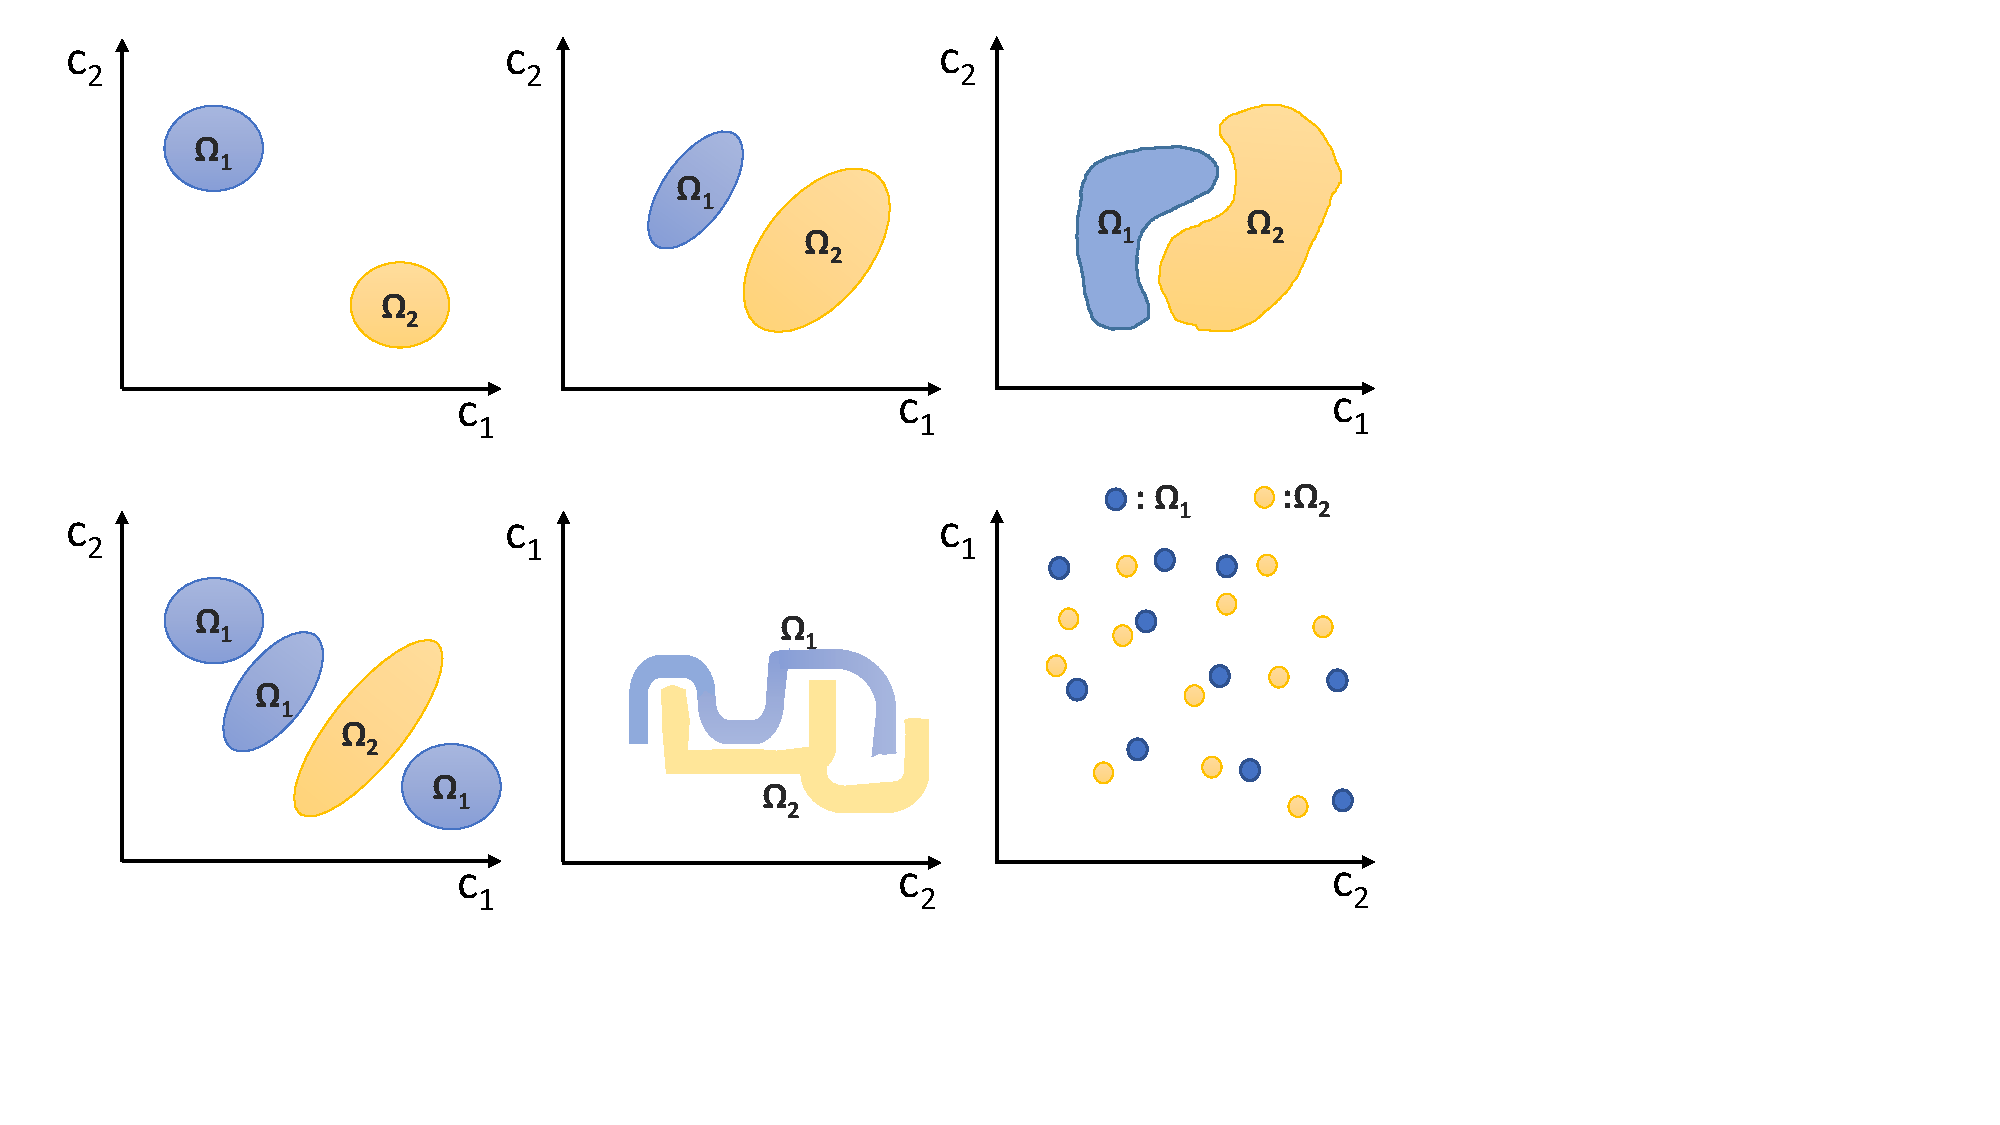
\includegraphics[width=.70\linewidth, trim={0  3cm 7cm 0cm},clip]{images/featurespace.pdf}
   \end{center}
\end{frame}


\begin{frame}
   \frametitle{Postulates for Pattern Recognition \cont}

   \begin{enumerate}
      \setcounter{enumi}{3}
      \item A (complex) pattern consists of \structure{simpler constituents}, which have certain relations to each other. A pattern may be decomposed into these constituents.\\[.3cm]
        \pause
      \item A (complex) pattern $\vec{f}(\vec{x}) \in \Omega$ has a certain \structure{structure}.
        Not any arrangement of simple constituents is a valid pattern. Many patterns may be represented with relatively few constituents.
   \end{enumerate}

   \begin{center}
      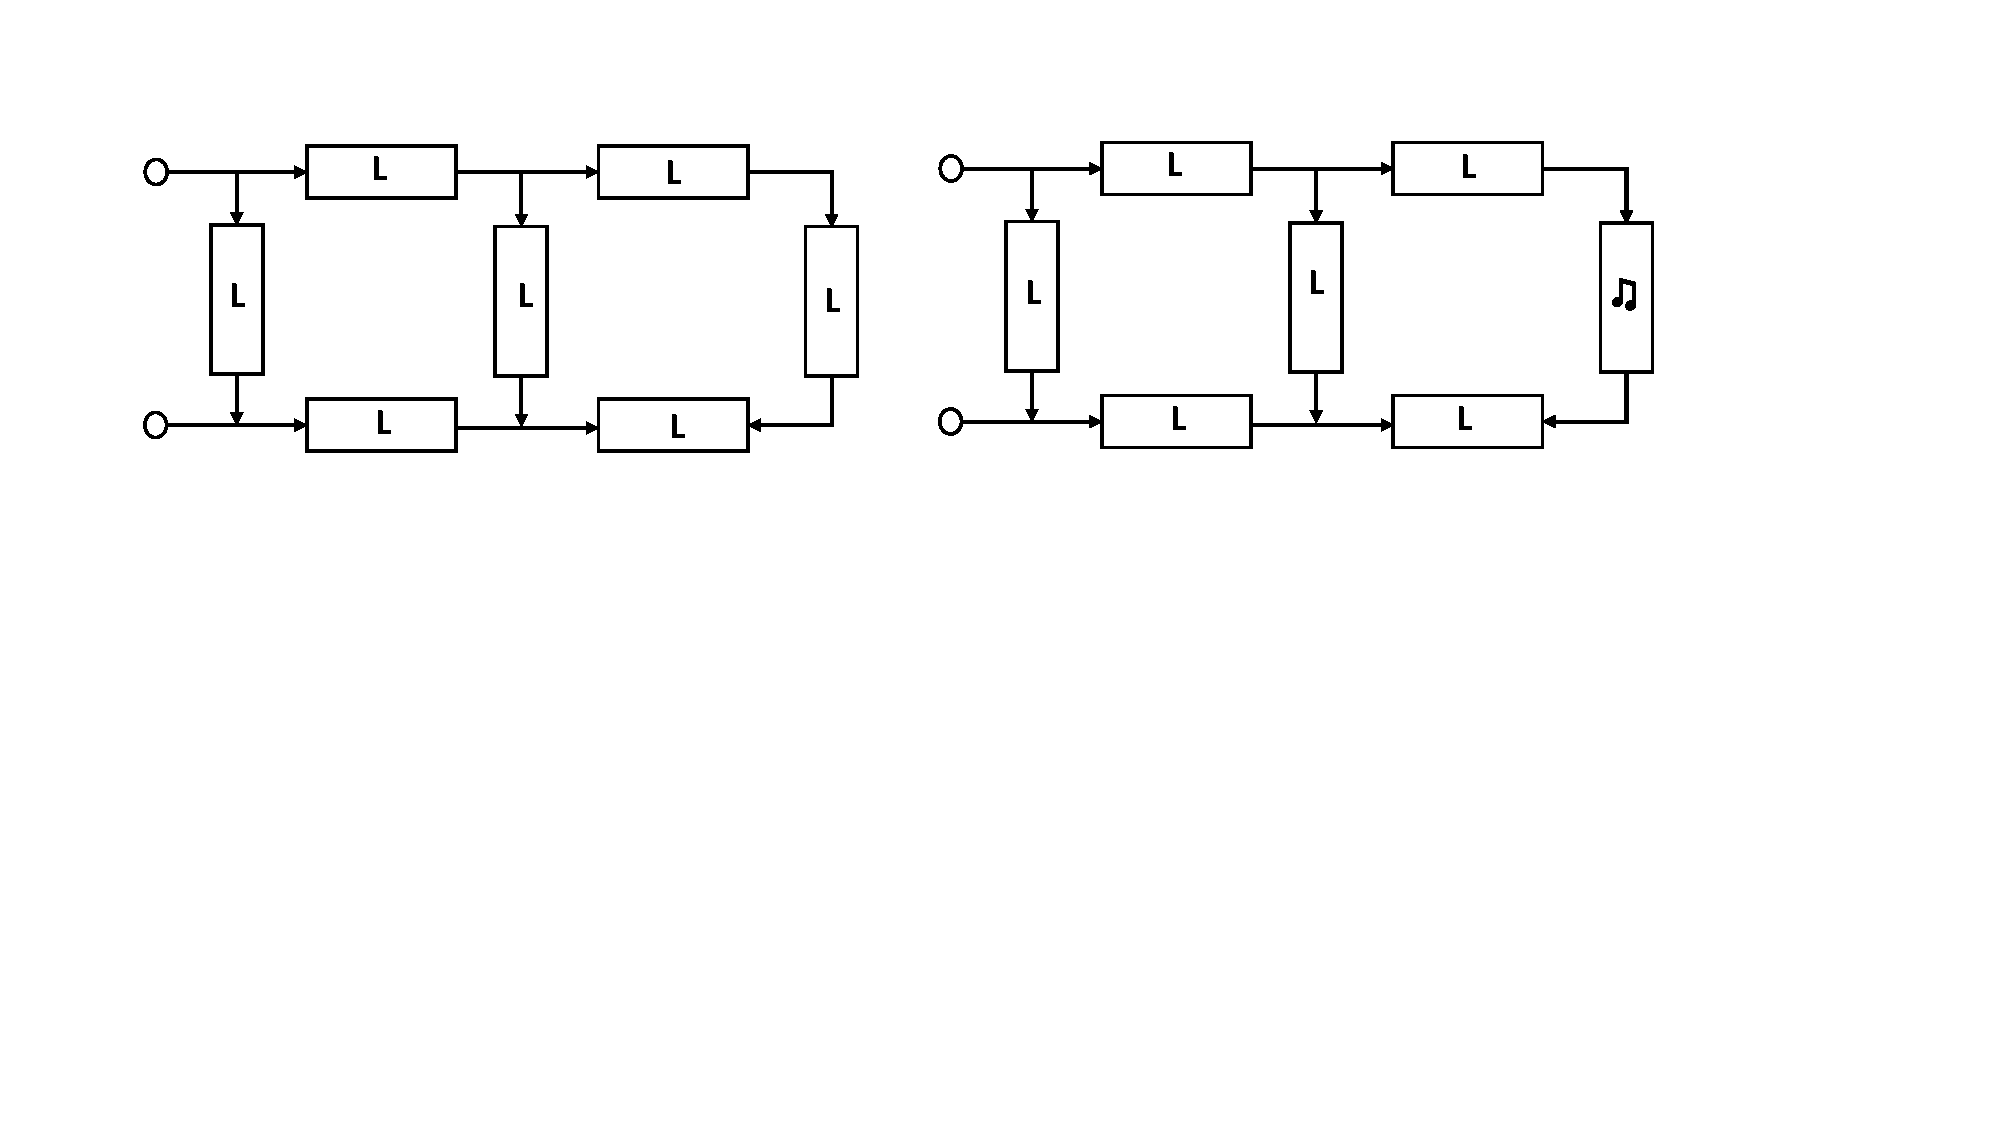
\includegraphics[width=\linewidth, trim={2cm 10cm 5cm 0cm},clip]{images/circuit.pdf}
   \end{center}
\end{frame}


\begin{frame}
   \frametitle{Postulates for Pattern Recognition \cont}

   \begin{enumerate}
      \setcounter{enumi}{5}
      \item Two patterns are \structure{similar} if their features or simpler constituents differ only lightly.
   \end{enumerate}
\end{frame}


\begin{frame}[fragile]
   \frametitle{Performance Evaluation}

   \begin{itemize}
      \item Feature vectors are used as input for the classifier
      \item Classifaction results in a discrete class index
      \item Confusion matrix:
   \end{itemize}

   \begin{table}
      \centering
      \small
      \newcommand{\C}[1]{$\Omega_{#1}$}
      \newcommand{\cc}[1]{$n_{#1}$}
      \newcommand{\CC}[1]{\multicolumn{1}{>{\columncolor[rgb]{0.8,0.8,0.8}}c}{\cc{#1}}}
      \begin{tabular}{c c | c c c c c | c}
          & \multicolumn{7}{c}{\structure{hypothesis}}                                                                            \\
          &                                            & \C{1}                 & \C{2}   & \C{3}   & \ldots   & \C{K}   & $\sum$  \\
         \cline{2-8}
         \multirow{5}{*}{\rotatebox{90}{\structure{reference}~~}}
          & \C{1}                                      & \CC{11}               & \cc{12} & \cc{13} & \ldots   & \cc{1K} & $N_{1}$ \\
          & \C{2}                                      & \cc{21}               & \CC{22} & \cc{23} & \ldots   & \cc{2K} & $N_{2}$ \\
          & \C{3}                                      & \cc{31}               & \cc{32} & \CC{33} & \ldots   & \cc{3K} & $N_{3}$ \\
          & \vdots                                     & \vdots                & \vdots  & \vdots  & $\ddots$ & \vdots  & \vdots  \\
          & \C{K}                                      & \cc{K1}               & \cc{K2} & \cc{K3} & \ldots   & \CC{KK} & $N_{K}$ \\
         \cline{2-8}
          & $\sum$                                     & \multicolumn{5}{c|}{} & $N$                                              \\
      \end{tabular}
      \caption{Confusion matrix with absolute frequencies for a $K$-class problem}
   \end{table}
\end{frame}


\begin{frame}[fragile]
   \frametitle{Performance Evaluation \cont}

   \structure{Evaluation of classifiers}

   \begin{itemize}
      \item Accuracy\,/\,Recognition Rate
           {\small
              \begin{displaymath}
                 \mathsf{RR} := \frac{1}{N} \sum_{\kappa=1}^{K}n_{\kappa\kappa} \cdot 100\,\%
              \end{displaymath}
              \pause
           }
      \item Recall and Precision
           {\small
              \begin{eqnarray*}
                 \mathsf{recall}_\kappa    & = & \frac{n_{\kappa\kappa}}{\sum_{i=1}^K n_{\kappa i}}
                 = \frac{n_{\kappa\kappa}}{N_\kappa} \\
                 \mathsf{precision}_\kappa & = & \frac{n_{\kappa\kappa}}{\sum_{i=1}^K n_{i \kappa}}
              \end{eqnarray*}
              \pause
           }
      \item (Unweighted) Average Recall
           {\small
              \begin{displaymath}
                 \mathsf{UAR} := \frac{1}{K} \sum_{\kappa=1}^K \frac{n_{\kappa\kappa}}{N_\kappa} \cdot 100\,\%
              \end{displaymath}
           }
   \end{itemize}
\end{frame}


\begin{frame}[fragile]
   \frametitle{Performance Evaluation \cont}

   \structure{Special case: only 2 classes}

   \begin{table}
      \centering
      \small
      \begin{tabular}{c c | c c |}
          & \multicolumn{1}{c}{}  & \multicolumn{2}{c}{\structure{Reference}}                         \\
          &                       & {\color{gr3}Positive}                     & {\color{gr3}Negative} \\
         \cline{2-4}
         \multirow{2}{*}{\rotatebox{90}{\structure{Hyp.}}}
          & {\color{gr3}Positive} & True Positive                             & False Positive        \\
          & {\color{gr3}Negative} & False Negative                            & True Negative         \\
         \cline{2-4}
      \end{tabular}
   \end{table}
   \spread

   \structure{Various performance measures:}

   \begin{itemize}
      \item True positive rate (hit rate, \structure{recall}, \structure{sensitivity}): $\frac{\#\mathsf{TP}}{\#\mathsf{TP} + \#\mathsf{FN}}$
      \item False positive rate (false alarm rate, fall-out): $\frac{\#\mathsf{FP}}{\#\mathsf{FP} + \#\mathsf{TN}}$
      \item Positive predictive value (\structure{precision}): $\frac{\#\mathsf{TP}}{\#\mathsf{TP} + \#\mathsf{FP}}$
      \item Negative predictive value: $\frac{\#\mathsf{TN}}{\#\mathsf{TN} + \#\mathsf{FN}}$
      \item True negative rate (\structure{specifity}): $\frac{\#\mathsf{TN}}{\#\mathsf{FP} + \#\mathsf{TN}}$ = 1 $-$ false positive rate
   \end{itemize}
\end{frame}


\begin{frame}[fragile]
   \frametitle{Performance Evaluation \cont}

   \structure{More performance measures:} \\[.3cm]

   \begin{itemize}
      \item Accuracy:
        {\small
        \begin{displaymath}
           \mathsf{ACC} = \frac{\#\mathsf{TP} + \#\mathsf{TN}}{\#\mathsf{TP} + \#\mathsf{FP} + \#\mathsf{FN} + \#\mathsf{TN}}
        \end{displaymath}
        }
        \spread

      \item F-measure: harmonic mean of recall and precision:
        {\small
        \begin{displaymath}
           F = \frac{2 \cdot \mathsf{recall} \cdot \mathsf{precision}}{\mathsf{recall} + \mathsf{precision}}
        \end{displaymath}
        }
   \end{itemize}
\end{frame}


\begin{frame}[fragile]
   \frametitle{Performance Evaluation \cont}

   \structure{Receiver Operating Characteristic (ROC) Curves}

   \begin{itemize}
      \item A classifier defines a single 2-d point in the ROC graph. \\[.7cm]
   \end{itemize}

   \begin{columns}
      \column{.4\linewidth}
      \resizebox{1.4\linewidth}{!}{
         \input{\texfigdir/roc.pstex_t}
      }
      %     
      \column{.6\linewidth}
      \footnotesize
      \vspace{-4.0cm}
      \begin{itemize}
         \item[(1)] Perfect classifier: no false positives, all negatives are classified as negatives
         \item[(2)] Random decision: half of positives are classified correctly, half of negatives are classified
           correctly
         \item[(3)] Low true positive rate, but lower false positive rate; strong evidence for positive classification
         \item[(4)] Here something goes really wrong!
      \end{itemize}
   \end{columns}
\end{frame}



\begin{frame}
   \frametitle{Performance Evaluation \cont}

   \structure{Example:} Classification of glaucoma based on eye pressure

   \begin{center}
      \includegraphics[width=.8\linewidth]{\jpgdir/gauss1d.\jpg}
   \end{center}
\end{frame}


\begin{frame}
   \frametitle{Performance Evaluation \cont}

   \begin{itemize}
      \item Classification is a threshold decision (in general $\theta = 0.5$)
      \item The true positive rate and the false positive rate can be computed for different thresholds $\theta \in [0,40]$
      \item Higher true positive rates for lower thresholds, \\
        but then higher false positive rates, too!
      \item The result is the ROC curve:
   \end{itemize}

   \begin{center}
      \resizebox{.35\linewidth}{!}{
         \input{\texfigdir/roc1.pstex_t}
      }
   \end{center}
\end{frame}


\begin{frame}
   \frametitle{Performance Evaluation \cont}

   \begin{itemize}
      \item Performance measure: \structure{area under curve} (AUC) \\[.3cm]
      \item The true positive rate and the false positive rate do not depend on the total number of samples.
      \item Hence, the ROC curve is independent of the priors of both classes \\
        (as opposed to recall-precision-curves).
   \end{itemize}
\end{frame}

\begin{frame}
   \frametitle{Types of Classifiers}

   \structure{Different types of classifiers:}

   \begin{itemize}
      \item Statistical
      \item Parametric
      \item Nonparametric
      \item Linear
      \item Nonlinear
      \item etc.
   \end{itemize}
\end{frame}


\begin{frame}
   \frametitle{Learning Phase}

   \begin{itemize}
      \item Classifier is only as good as the training samples
      \item The more training samples the better! \\[.5cm]
      \item Distinction between \structure{supervised} and \structure{unsupervised} learning\\[.5cm]
      \item Computational complexity of the classifier may depend on the size of the training set
   \end{itemize}
\end{frame}


{
\usebackgroundtemplate{\includegraphics[width=\paperwidth]{png/nextTime.png}}
\begin{frame}[plain]
\end{frame}
}


\ifnosummary
   \subsection{Literature}

   \begin{frame}
      \frametitle{Literature}

      \begin{columns}

         \column{.8\linewidth}
         \small
         \vspace{-1.25cm}
         \begin{itemize}
            \item Richard O. Duda, Peter E. Hart, David G. Stock: \\
              \structure{Pattern Classification}, 2nd edition, \\
              John Wiley \& Sons, New York, 2001, EUR 114.45 \\[.5cm]

            \item Trevor Hastie, Robert Tibshirani, Jerome Friedman: \\
              \structure{The Elements of Statistical Learning -- \\
                 Data Mining, Inference, and Prediction}, \\
              2nd edition, Springer, New York, 2009, EUR 71.05 \\
              {\small \url{http://www-stat.stanford.edu/~tibs/ElemStatLearn/}} \\[.5cm]

            \item Christopher M.\ Bishop: \\
              \structure{Pattern Recognition and Machine Learning}, \\
              Springer, New York, 2006, EUR 75.05
         \end{itemize}

         \column{.2\linewidth}
         \includegraphics[width=.5\linewidth]{\jpgdir/duda.\jpg} \\[.5cm]
         \includegraphics[width=.5\linewidth]{\jpgdir/hastie.\jpg} \\[.4cm]
         \includegraphics[width=.5\linewidth]{\jpgdir/bishop.\jpg}
      \end{columns}
   \end{frame}


   \begin{frame}
      \frametitle{Further Readings}

      \begin{itemize}
         \item Richard O. Duda, Peter E. Hart, David G. Stock: \\
           \structure{Pattern Classification}, 2nd edition, \\
           John Wiley \& Sons, New York, 2001, EUR 114.45 \\[.5cm]
         \item H.\ Niemann: \\
           \structure{Klassifikation von Mustern} \\
           2. \"{u}berarbeitete Auflage, 2003 \\
           {\small \url{http://www5.informatik.uni-erlangen.de/fileadmin/Persons/NiemannHeinrich/klassifikation-von-mustern/m00links.html}}
      \end{itemize}
   \end{frame}
\fi

\subsection{Comprehensive Questions}

\begin{frame}
   \frametitle{Comprehensive Questions}

   \begin{itemize}
      \item What are features vectors? \\[.7cm] \pause
      \item What are the postulates of pattern recognition? \\[.7cm] \pause
      \item Why do we need training samples? \\[.7cm] \pause
      \item How can we test the performance of our classifier?
   \end{itemize}
\end{frame}


  \setcounter{section}{1} \section{Pattern Recognition Basics}

\subsection{Classification of Simple Patterns}

\begin{frame}
	\frametitle{Classification of Simple Patterns}

	The system for the classification of simple patterns has the following generic structure\\
	\vspace{2cm}
	\pause
%\begin{centering}
	$\hspace{1.03cm} \overset{\vec f}{\longrightarrow}\fbox{Preprocessing}\overset{\vec g}{\longrightarrow}\fbox{Feature Extraction} \overset{\vec c}{\longrightarrow}\fbox{Classification} \overset{y}{\longrightarrow}$\\
	$\hspace{1.03cm}\hspace{8.5cm} \uparrow $\\
	$\hspace{1.03cm}\hspace{4.3cm} \fbox{Training Samples}\longrightarrow \fbox{Learning}$
\end{frame}

\begin{frame}
	\frametitle{Classification of Simple Patterns \cont}

	\begin{itemize}
		\item {\em \structure{Supervised learning:}}

		      $m$ training samples include feature and associated class number
		      \begin{displaymath}
			      S = \{ (\vec x_1, y_1), (\vec x_2, y_2), (\vec x_3, y_3), \dots, (\vec x_m, y_m) \}
		      \end{displaymath}
              where $\vec x_i \in \mathcal{X}$ denotes the feature vector and $y_i\in Z$ denotes the class number of sample $i$.
	      If nothing special is mentioned ${\mathcal{X}}\subseteq \mathbb{R}^d$.
		      \pause
		      \vspace{0.5cm}
		\item {\em \structure{Unsupervised learning:}}

		      $m$ training samples just include features, no class assignments and even the number of classes is (not always) known
		      \begin{displaymath}
			      S = \{ \vec x_1, \vec x_2, \vec x_3, \dots, \vec x_m \}
		      \end{displaymath}
	\end{itemize}
\end{frame}


\subsection{Bayesian Classifier}

\begin{frame}
	\frametitle{Bayesian Classifier}

	\structure{Notation:}

	\begin{center}
		\begin{minipage}{0.7\textwidth}
			\begin{itemize}
				\item[ $ \vec x \in \mathbb{R}^d:$]  $d$-dimensional feature vector
				\item[ $y:$] class number \\
				      (usually $y\in\{0,1\}$ or $y\in\{-1,+1\}$)
				\item[$p(y):$] prior probability of pattern class $y$
				\item[$p(\vec x):$] evidence\\
				      (distribution of features in $d$-dimensional feature space)
				\item[$p(\vec x , y):$] joint probability density function (pdf)
				\item[$p(\vec x |y):$] class conditional density
				\item[$p(y| \vec x):$] posterior probability
			\end{itemize}
		\end{minipage}
	\end{center}
\end{frame}


\begin{frame}
	\frametitle{Bayesian Classifier \cont}
\vspace{-.52cm}
  \begin{figure}
    \resizebox{.85\linewidth}{!}{
      \alt<25->{
        \includegraphics[width=.85\linewidth]{\pngdir/condProb/Folie25.\png}
      }{\alt<24>{
        \includegraphics[width=.85\linewidth]{\pngdir/condProb/Folie24.\png}
      }{\alt<23>{
        \includegraphics[width=.85\linewidth]{\pngdir/condProb/Folie23.\png}
      }{\alt<22>{
        \includegraphics[width=.85\linewidth]{\pngdir/condProb/Folie22.\png}
      }{\alt<21>{
        \includegraphics[width=.85\linewidth]{\pngdir/condProb/Folie21.\png}
      }{\alt<20>{
        \includegraphics[width=.85\linewidth]{\pngdir/condProb/Folie20.\png}
      }{\alt<19>{
        \includegraphics[width=.85\linewidth]{\pngdir/condProb/Folie19.\png}
      }{\alt<18>{
        \includegraphics[width=.85\linewidth]{\pngdir/condProb/Folie18.\png}
      }{\alt<17>{
        \includegraphics[width=.85\linewidth]{\pngdir/condProb/Folie17.\png}
      }{\alt<16>{
        \includegraphics[width=.85\linewidth]{\pngdir/condProb/Folie16.\png}
      }{\alt<15>{
        \includegraphics[width=.85\linewidth]{\pngdir/condProb/Folie15.\png}
      }{\alt<14>{
        \includegraphics[width=.85\linewidth]{\pngdir/condProb/Folie14.\png}
      }{\alt<13>{
        \includegraphics[width=.85\linewidth]{\pngdir/condProb/Folie13.\png}
      }{\alt<12>{
        \includegraphics[width=.85\linewidth]{\pngdir/condProb/Folie12.\png}
      }{\alt<11>{
        \includegraphics[width=.85\linewidth]{\pngdir/condProb/Folie11.\png}
      }{\alt<10>{
        \includegraphics[width=.85\linewidth]{\pngdir/condProb/Folie10.\png}
      }{\alt<9>{
        \includegraphics[width=.85\linewidth]{\pngdir/condProb/Folie9.\png}
      }{\alt<8>{
        \includegraphics[width=.85\linewidth]{\pngdir/condProb/Folie8.\png}
      }{\alt<7>{
        \includegraphics[width=.85\linewidth]{\pngdir/condProb/Folie7.\png}
      }{\alt<6>{
        \includegraphics[width=.85\linewidth]{\pngdir/condProb/Folie6.\png}
      }{\alt<5>{
        \includegraphics[width=.85\linewidth]{\pngdir/condProb/Folie5.\png}
      }{\alt<4>{
        \includegraphics[width=.85\linewidth]{\pngdir/condProb/Folie4.\png}
      }{\alt<3>{
        \includegraphics[width=.85\linewidth]{\pngdir/condProb/Folie3.\png}
      }{\alt<2>{
        \includegraphics[width=.85\linewidth]{\pngdir/condProb/Folie2.\png}
      }{
        \includegraphics[width=.85\linewidth]{\pngdir/condProb/Folie1.\png}
      }}}}}}}}}}}}}}}}}}}}}}}}
    }
  \end{figure}

\end{frame}

\begin{frame}
	\frametitle{Bayesian Classifier \cont}

	\structure{Bayes rule:}\\[.5cm]

	\begin{eqnarray*}
		\underbrace{p(\vec x , y)}_{joint\ pdf}
		&=& \pause \underbrace{p(y)}_{prior} \cdot \underbrace{p(\vec x | y)}_{class\ conditional\ pdf} \\[.5cm] \pause
		&=& \underbrace{ p(\vec x)}_{evidence} \cdot \underbrace{ p(y| \vec x)}_{posterior}
	\end{eqnarray*}
\end{frame}


\begin{frame}
	\frametitle{Bayesian Classifier \cont}

	Now we get the posterior as follows:

	\begin{eqnarray*}
		p(y| \vec x)
		&=& \pause \frac{p(y) \cdot p(\vec x | y)}{p(\vec x)} \\ \pause
		&=& \frac{p(y) \cdot p(\vec x | y)}{\sum\limits_{y'}p(\vec x , y')} \\ \pause
		&=& \frac{p(y) \cdot p(\vec x | y)}{\sum\limits_{y'}p(y') \cdot p(\vec x | y')}\\
	\end{eqnarray*}
\end{frame}


\begin{frame}
	\frametitle{Bayesian Classifier \cont}

	\structure{Note:}
	\begin{displaymath}
		p(\vec x) = \sum\limits_{y}p(y) \cdot p(\vec x | y)
	\end{displaymath}
	is a \structure{marginal} of $p(\vec x , y)$.

	\begin{itemize}
		\item We get $p(\vec{x})$ by marginalizing $p(\vec{x}, y)$ over $y$.
		\item Accordingly we get $p(y)$ by marginalizing $p(\vec{x}, y)$ over $\vec{x}$, i.\,e.
		      \begin{eqnarray*}
			      p(y)&=& \int p(\vec{x}, y) \mathsf{d}\vec{x}
		      \end{eqnarray*}
	\end{itemize}

	\alert{Did you notice:} $y$ is a discrete random variable whereas $\vec{x}$ is a continuous random vector (summation vs.\ integration).
\end{frame}


{
\usebackgroundtemplate{\includegraphics[width=\paperwidth]{png/nextTime.png}}
\begin{frame}[plain]
\end{frame}
}


\begin{frame}
	\frametitle{Bayesian Classifier \cont}

	Now let us summarize the Bayesian decision rule:\\[.3cm]
	We decide for the class $y^*$ according to the decision rule
	\begin{eqnarray*}
		y^* &=& \pause \argmax\limits_{y} p(y | \vec x)\ \\[.3cm] \pause
		&=& \argmax\limits_{y} \frac{p(y) \cdot p(\vec x | y)}{p(\vec x)} \\[.3cm] \pause
		&=& \argmax\limits_{y} p(y) \cdot p(\vec x | y) \\[.3cm] \pause
		&=& \argmax\limits_{y} \{\log p(y)\ + \log p(\vec x | y)\}
	\end{eqnarray*}
\end{frame}


\begin{frame}
	\frametitle{Bayesian Classifier \cont}

	\structure{Notes:} \\[.3cm]

	\begin{itemize}
		\item The key aspect in designing a classifier is to find a good model \\
		      for the posterior $p(y|\vec x)$. \\[.3cm]
		\item Feature vectors $\vec x$ usually have fixed dimensions $d$ in simple classification schemes, \\[.3cm]
		\item but ${\mathcal{X}}$ is not necessarily a subset of $\mathbb{R}^d$: \\
		      features of varying dimension, sequences and sets of features
	\end{itemize}
\end{frame}


\begin{frame}
	\frametitle{Bayesian Classifier \cont}

	\begin{itemize}
		\item \structure{Generative modeling:} \\
		      modeling and estimation of $p(y)$ and $p(\vec x | y)$. \\[.5cm]
		\item \structure{Discriminative modeling:} \\
		      straight modeling and estimation of $p(y|\vec x)$.
	\end{itemize}
\end{frame}


\subsection{Optimality of the Bayesian Classifier}

\begin{frame}
	\frametitle{Optimality of the Bayesian Classifier}

	%  \begin{citeblock}{Definition}
	\begin{definition}
		$l(y_{1},y_{2})$ is the \structure{loss} if a feature vector belonging to class $y_{2}$
		is assigned to class $y_{1}$. The $(0,1)$-loss function is defined by
		\begin{eqnarray*}
			l(y_{1},y_{2}) &= &\left\{ \begin{array}{cc}
				0 & ,\ if\ y_{1}=y_{2} \\
				1 & ,\ otherwise
			\end{array} \right.
		\end{eqnarray*}
		%  \end{citeblock}
	\end{definition}
\end{frame}


\begin{frame}
	\frametitle{Optimality of the Bayesian Classifier \cont}

	The \structure{best (or optimal) decision rule} according to classification loss minimizes the average loss L:

	\begin{eqnarray*}
		\mathsf{AL}(\vec x , y) &=& \sum\limits_{y'}l(y,y')p(y'|\vec x)
	\end{eqnarray*}

\end{frame}


\begin{frame}
	\frametitle{Optimality of the Bayesian Classifier \cont}

	Using the $(0,1)$-loss function, the class decision is based on:

	\begin{eqnarray*}
		y^* &=& \argmin\limits_{y} \mathsf{AL}(\vec x, y)\\
		\pause  &=& \argmin\limits_{y} \sum\limits_{y'} l(y,y') \cdot p(y'|\vec x)\\
		%           \pause  &=& \argmin\limits_{y} (1-p(y|\vec x))\\
		\pause  &=& \argmax\limits_{y} p(y|\vec x)\\
	\end{eqnarray*}
\end{frame}


\begin{frame}
	\frametitle{Optimality of the Bayesian Classifier \cont}

	\structure{Conclusion:}

	\begin{itemize}
		\item The optimal classifier w.\,r.\,t.\ the (0,1)-loss function applies the Bayesian decision rule.
		\item This classifier is called \structure{Bayesian classifier}. \\[.75cm]
	\end{itemize}
	\spread

	\vorsicht The loss function is {\bf NOT} convex. \vfill
\end{frame}


\subsection{Lessons Learned}

\begin{frame}
	\frametitle{Lessons Learned}

	\begin{itemize}
		\item General structure of a classification system \\[.5cm] \pause
		\item Supervised and unsupervised learning \\[.5cm] \pause
		\item Basics on probabilities (probability, pdf, Bayes rule, etc.) \\[.5cm] \pause
		\item Optimality of Bayes classifier and the role of the loss function \\[.5cm] \pause
		\item Discriminative and generative approach to model a posteriori probability
	\end{itemize}
\end{frame}

{
\usebackgroundtemplate{\includegraphics[width=\paperwidth]{png/nextTime.png}}
\begin{frame}[plain]
\end{frame}
}


\subsection{Further Readings}

\begin{frame}
	\frametitle{Further Readings}

	\begin{itemize}
		\item Heinrich Niemann: \\
		      \structure{Pattern Analysis}, \\
		      Springer Series in Information Sciences 4, Springer, Berlin, 1982. \\[.15cm]
		\item Heinrich Niemann: \\
		      \structure{Klassifikation von Mustern}, \\
		      Springer Verlag, Berlin, 1983. \\[.15cm]
		\item Richard O. Duda, Peter E. Hart, David G. Stork: \\
		      \structure{Pattern Classification}, 2nd Edition, \\
		      John Wiley \& Sons, New York, 2000.
	\end{itemize}
\end{frame}

 
  \setcounter{section}{2} \section{Logistic Regression I}

\begin{frame}
  \frametitle{Logistic Regression}

  Logistic Regression is a \structure{discriminative model}, because it models \\
  the posterior probabilities $p(y|\vec{x})$ directly.
\end{frame}


\subsection{Posteriors and the Logistic Function}

\begin{frame}
  \frametitle{Posteriors and the Logistic Function}
 
  For two classes $y\in\{0, 1\}$ we get:
  
  \begin{eqnarray*}
    p(y=0| \vec x) 
      &=& \pause \frac{p(y=0) \cdot p(\vec x | y=0)}{p(\vec x)} \\[.5cm] \pause 
      &=& \frac{p(y=0) \cdot p(\vec x | y=0)}{p(y=0)p(\vec x |y=0)+p(y=1)p(\vec x| y=1)} \\[.5cm] \pause
      &=& \frac{1}{1+\frac{p(y=1)p(\vec x| y=1)}{p(y=0)p(\vec x| y=0)}}
  \end{eqnarray*}
\end{frame}
 
 
\begin{frame}
  \frametitle{Posteriors and the Logistic Function \cont}

  \begin{eqnarray*}
    p(y=0| \vec x) 
      &=& \frac{1}{1+\frac{p(y=1)p(\vec x| y=1)}{p(y=0)p(\vec x| y=0)}} \\[.3cm] \pause
      &\phantom{=}& \mbox{\small (\structure{Trick:} extend with exponential and logarithm)} \\[.3cm] \pause
      &=& \frac{1}{1+e^{\log \frac{p(y=1)p(\vec x| y=1)}{p(y=0)p(\vec x| y=0)} } } \\[.3cm] \pause
      &=& \frac{1}{1+e^{-\log\frac{p(y=0)}{p(y=1)} - \log\frac{p(\vec x| y=0)}{p(\vec x|y=1)}}}\\[0.3cm] \pause
      &=& \frac{1}{1+e^{-\log\frac{p(y=0|\vec x)}{p(y=1|\vec x)}}}
  \end{eqnarray*}
\end{frame}


\begin{frame}
  \frametitle{Posteriors and the Logistic Function \cont}

  We see that the posterior for class $y = 0$ can be written in terms of \\
  a \structure{logistic function}:
%
  \begin{eqnarray*}
    p(y=0| \vec x) &=& \frac{1}{1+e^{-F(\vec{x})}}
  \end{eqnarray*}
  \pause

  And thus the posterior for the other class $y = 1$:
%
  \begin{eqnarray*}
    p(y=1| \vec x) &=& \pause 1- p(y=0| \vec x) \\[.3cm] \pause
                   &=& \frac{e^{-F(\vec x)}}{1+e^{-F(\vec{x})}} \\[.3cm] \pause
                   &=&  \frac{1}{1+e^{F(\vec{x})}}
  \end{eqnarray*}
\end{frame}


\begin{frame}
  \frametitle{Posteriors and the Logistic Function \cont}

  \begin{citeblock}{Definition}

    The {\em logistic function} (also called {\em sigmoid function}) is defined by
    \begin{eqnarray*}
      g(x) &=& \frac{1}{1+e^{-x}}
    \end{eqnarray*}
    where $x\in \real$.
  \end{citeblock}
\end{frame}


\begin{frame}
  \frametitle{Posteriors and the Logistic Function \cont}

  The derivative of the sigmoid function fulfills the nice property:

  \begin{eqnarray*}
    g'(x) &=& \left( \frac{1}{1+e^{-x}} \right)' = \pause \left( (1+e^{-x})^{-1}\right)'= \pause \frac{1}{(1+e^{-x})^2}\cdot e^{-x} \\[.3cm] \pause
          &=& \frac{1}{(1+e^{-x})} \cdot \frac{e^{-x}}{(1+e^{-x})} \\[.3cm] \pause
          &=& \frac{1}{(1+e^{-x})} \cdot \frac{1}{(1+e^{x})} \\[.3cm] \pause
          &=& g(x)g(-x) \\[.3cm] \pause
          &=& g(x)(1-g(x)) \quad.
  \end{eqnarray*}
\end{frame}


\begin{frame}
  \frametitle{Posteriors and the Logistic Function \cont}
 
  \begin{figure}
    \resizebox{.85\linewidth}{!}{
      \alt<4->{
        \input{\texfigdir/sigmoid4.pstex_t}
      }{\alt<3>{
        \input{\texfigdir/sigmoid3.pstex_t}
      }{\alt<2>{
        \input{\texfigdir/sigmoid2.pstex_t}
      }{
        \input{\texfigdir/sigmoid1.pstex_t}
      }}}
    }
    \caption{Sigmoid function: $g(ax)=1/(1+e^{-ax})$ for $a=1,2,3,4$}
    \label{f:sigmoid}
  \end{figure}
\end{frame}


{
\usebackgroundtemplate{\includegraphics[width=\paperwidth]{png/nextTime.png}}
\begin{frame}[plain]
\end{frame}
}


\subsection{Decision Boundary}

\begin{frame}
  \frametitle{Decision Boundary}

  The \structure{decision boundary} $\delta(\vec x)=0$ (zero level set) in feature space separates the two classes. \\[.3cm]
  Points $\vec x$ on the decision boundary satisfy:
 
  \begin{eqnarray*}
    {p(y=0|\vec{x})}&=& {p(y=1|\vec x)}
  \end{eqnarray*}
 
  and thus
 
  \begin{eqnarray*}
    \log \frac{p(y=0|\vec{x})}{p(y=1|\vec x)} &=& \pause \log 1 = 0 \quad.
  \end{eqnarray*}
\end{frame}


\begin{frame}
  \frametitle{Decision Boundary \cont}
 
  \begin{lemma}
    The decision boundary is given by $F(\vec x) = 0$.
  \end{lemma}
  \pspread
 
  \structure{Proof:}
%
  \begin{eqnarray*}
    \log \frac{p(y=0|\vec{x})}{p(y=1|\vec x)} &=& F(\vec x) = 0\\[.3cm] \pause
    \frac{p(y=0|\vec{x})}{p(y=1|\vec x)} &=& e^{F(\vec x)} \\[.3cm] \pause
    {p(y=0|\vec{x})}&=& e^{F(\vec x)} {p(y=1|\vec x)} \\[.3cm]
    % {p(y=0|\vec{x})}&=& e^{F(\vec x)}\left( {1-p(y=0|\vec x)}\right)
  \end{eqnarray*} 
\end{frame}


\begin{frame}
  \frametitle{Decision Boundary \cont}
 
  Now we use that the posteriors sum up to one:
  
  \begin{eqnarray*}
    {p(y=0|\vec{x})}&=& e^{F(\vec x)}\left( {1-p(y=0|\vec x)}\right) \\ \\
    \pause {p(y=0|\vec{x})}&=& \frac{e^{F(\vec x)}}{1+e^{F(\vec x)}} \\ \\
    \pause {p(y=0|\vec{x})}&=& \frac{1}{1+e^{-F(\vec x)}} 
  \end{eqnarray*} 
\end{frame}


\begin{frame}
  \frametitle{Decision Boundary \cont}
 
  \begin{figure}
    \resizebox{1\linewidth}{!}{
      \alt<4->{
        \input{\texfigdir/logit3.pstex_t}
      }{\alt<3>{
        \input{\texfigdir/logit2.pstex_t}
      }{\alt<2>{
        \input{\texfigdir/logit1.pstex_t}      
      }{
        \input{\texfigdir/logit0.pstex_t}
      }}}
    }
    \caption{Two Gaussians and their posteriors: {\color{bl3} $\sigma_0$}={\color{gr3}$ \sigma_1$}= 0.25,  {\color{bl3} $\mu_0=-2$},
              {\color{gr3} $\mu_1=1$}}
    \label{f:logit}
  \end{figure}
\end{frame}


\begin{frame}
  \frametitle{Decision Boundary \cont}
  
  \begin{ovalblock}{Example}
    \footnotesize
    Let us assume both classes have normally distributed $d$-dimensional feature vectors:
 
    \begin{eqnarray*}
      p(\vec x | y) &=& \frac{1}{ \sqrt{ \det{(2 \pi \mat{\Sigma}_y})} } 
                        e^{-\frac{1}{2} (\vec{x} - \vec{\mu}_y)^T \mat{\Sigma}_y^{-1} (\vec{x} - \vec{\mu}_y)  }
    \end{eqnarray*}
    \pause
 
    Then we can write the posterior of $y=0$ in terms of a logistic function:
 
    \begin{eqnarray*}
      p(y=0|\vec x) &=& \frac{1}{1+e^{-F(\vec x)}} = \frac{1}{1+e^{ - \left( \vec x^T \mat A \vec x + \vec \alpha^T\vec x + \alpha_0 \right) } } \\ \\
      \pause F(\vec x) &=& \log \frac{p(y=0|\vec x)}{p(y=1|\vec x)} = \log \frac{p(y=0)p(\vec x | y=0) }{p(y=1)p(\vec x|y =1)}
    \end{eqnarray*}
  \end{ovalblock}
\end{frame}


\begin{frame}
  \frametitle{Decision Boundary \cont}

  \begin{ovalblock}{Example cont.}
    \footnotesize
    \begin{eqnarray*}
      F(\vec x) &=&
        \log\frac{p(y=0)}{p(y=1)} +
        \log
        \frac{
          \frac{1}{ \sqrt{ \det{( 2 \pi \mat{\Sigma}_0)}} }
          e^{ -\frac{1}{2} (\vec{x} - \mat{\mu}_0)^T \mat{\Sigma}_0^{-1} (\vec{x} - \vec{\mu}_0) }         
        }{
          \frac{1}{ \sqrt{ \det{(2 \pi \mat{\Sigma}_1)}} }
          e^{ -\frac{1}{2} (\vec{x} - \vec{\mu}_1)^T \mat{\Sigma}_1^{-1} (\vec{x} - \vec{\mu}_1)}
        }
    \end{eqnarray*}
    \pause
 
    This function has the constant component:
% 
    \begin{eqnarray*}
      c &=& \log \frac{p(y=0)}{p(y=1)}+\frac{1}{2}
            \log \frac{ { \det{(2\pi\mat{\Sigma}_1)}}}
                      { { \det{(2\pi\mat{\Sigma}_0)}}}
    \end{eqnarray*}
    \pause 
    
    We observe:
    \begin{itemize}
      \small
      \item Priors imply a constant offset of the decision boundary. 
      \item If priors and covariance matrices of both classes are identical, this offset is $c=0$.
    \end{itemize}
  \end{ovalblock}
\end{frame}


\begin{frame}
  \frametitle{Decision Boundary \cont}

  \begin{ovalblock}{Example cont.}
    \small
    Furthermore we have:
    \begin{eqnarray*}
      \log{ 
        \frac{e^{ - \frac{1}{2} (\vec{x} - \vec{\mu}_0)^T \mat{\Sigma}_0^{-1} (\vec{x} - \vec{\mu}_0)} }
             {e^{ - \frac{1}{2} (\vec{x} - \vec{\mu}_1)^T \mat{\Sigma}_1^{-1} (\vec{x} - \vec{\mu}_1)} }
      } & = & \\[.3cm]
      & & \pause \hspace{-5cm} =
      \frac{1}{2} 
      \left(
        (\vec{x} - \vec{\mu}_1)^T \mat{\Sigma}_1^{-1} (\vec{x} - \vec{\mu}_1) - (\vec{x} - \vec{\mu}_0)^T \mat{\Sigma}_0^{-1} (\vec{x} - \vec{\mu}_0)
      \right) \\[.3cm]
      & & \hspace{-5cm} \pause =
      \frac{1}{2} 
      \left(
        \vec{x}^T (\mat{\Sigma}_1^{-1} - \mat{\Sigma}_0^{-1}) \vec{x} 
        -2 (\vec{\mu}_1^T \mat{\Sigma}_1^{-1} - \vec{\mu}_0^T \mat{\Sigma}_0^{-1} ) \vec{x} + \right.\\
        & & \left. \hspace{-4cm} 
        + \vec{\mu}_1^T \mat{\Sigma}_1^{-1} \vec{\mu}_1 - \vec{\mu}_0^T \mat{\Sigma}_0^{-1} \vec{\mu}_0
      \right)
    \end{eqnarray*}
  \end{ovalblock}
\end{frame}
 
 
\begin{frame}
  \frametitle{Decision Boundary \cont}
  
  \begin{ovalblock}{Example cont.}
    \small
    Now we have:
    \begin{eqnarray*}
      \mat{A}        &=& \frac{1}{2} (\mat{\Sigma}_1^{-1} - \mat{\Sigma}_0^{-1}) \\[.5cm]
      \vec{\alpha}^T &=& \vec{\mu}_0^T \mat{\Sigma}_0^{-1} - \vec{\mu}_1^T \mat{\Sigma}_1^{-1} \\[.5cm]
      \alpha_0       &=& \log \frac{p(y=0)}{p(y=1)} + \frac{1}{2}
                         \left(
                           \log
                             \frac{ \det{( 2 \pi \mat{\Sigma}_1)}}
                                  { \det{( 2 \pi \mat{\Sigma}_0)}} + 
                             \vec{\mu}_1^T \mat{\Sigma}_1^{-1} \vec{\mu}_1 -
                             \vec{\mu}_0^T \mat{\Sigma}_0^{-1} \vec{\mu}_0
                         \right)
    \end{eqnarray*}
  \end{ovalblock}
\end{frame}
  
  
\begin{frame}
  \frametitle{Decision Boundary \cont}
  
  \begin{figure}
    
    \resizebox{.6\linewidth}{!}{
      \alt<4->{
        \input{\texfigdir/plot_decision_boundary.pstex_t}
      }
{\alt<3>{
        \input{\texfigdir/gaussian2.pstex_t}
      }{\alt<2>{
        \input{\texfigdir/gaussian1.pstex_t}
      }{
        \input{\texfigdir/gaussian0.pstex_t}
      }}}
    }
    \caption{Two Gaussian sample sets and the decision boundary}
  \end{figure}
\end{frame}
 
 
\begin{frame}
  \frametitle{Decision Boundary \cont}

  \structure{Quadratic polynomials in the 2 variables $x_1$ and $x_2$}

  \begin{eqnarray*}
    F(\vec{x}) 
      &=& \vec x^T \mat A \vec x + \vec \alpha^T\vec x + \alpha_0 \\
      &=& a x_1^2 + b x_1 x_2 + c x_2^2 + d x_1 + e x_2 + f \stackrel{!}{=} 0
  \end{eqnarray*}
  \vspace{-0.75cm}

  \begin{figure}
  \copyrightbox[b]{
    \subfloat[circles and ellipses]{
      \makebox[.3\linewidth]{
        \href{http://en.wikipedia.org/wiki/File:Conic_sections_with_plane.svg}{
          \includegraphics[height=3cm]{\pngdir/conic_section_circle_ellipse.\png}
        }
      }
    }
    \subfloat[parabolas]{
      \makebox[.3\linewidth]{
        \href{http://en.wikipedia.org/wiki/File:Conic_sections_with_plane.svg}{
          \includegraphics[height=3cm]{\pngdir/conic_section_parabola.\png}
        }
      }
    }
    \subfloat[hyperbolas]{
      \makebox[.3\linewidth]{
        \href{http://en.wikipedia.org/wiki/File:Conic_sections_with_plane.svg}{
          \includegraphics[height=3cm]{\pngdir/conic_section_hyperbola.\png}
        }
      }
    }
  }{Pbroks13,  \href{https://creativecommons.org/licenses/by/3.0} {CC BY 3.0}, via Wikimedia Commons}
  \end{figure}
\end{frame}


\begin{frame}
  \frametitle{Decision Boundary \cont}

  \structure{Posterior probability}

  \begin{center}
    \resizebox{.85\linewidth}{!}{
      \input{\texfigdir/plot_posterior.pstex_t}
    }
  \end{center}
\end{frame}

{
\usebackgroundtemplate{\includegraphics[width=\paperwidth]{png/nextTime.png}}
\begin{frame}[plain]
\end{frame}
}

 
\begin{frame}
  \frametitle{Decision Boundary in Distributions with Equal Dispersion}
 
  \begin{ovalblock}{Example cont.}
    \small
    If both classes share the same covariances i.\,e.\ $\mat\Sigma= \mat\Sigma_0=\mat\Sigma_1$, then the argument of the sigmoid function is linear in the components of $\vec{x}$.
   
    \begin{eqnarray*}
      \mat{A}        &=& \mat{0} \\[.5cm]
      \vec{\alpha}^T &=& (\vec{\mu}_0 - \vec{\mu}_1)^T \mat{\Sigma}^{-1} \\[.5cm]
      \alpha_0       &=& \log \frac{p(y=0)}{p(y=1)} + 
                         \frac{1}{2}(\vec{\mu}_1 - \vec{\mu}_0)^T \mat{\Sigma}^{-1} (\vec{\mu}_1 - \vec{\mu}_0)  
     \end{eqnarray*}
  \end{ovalblock}
\end{frame}


\begin{frame}
  \frametitle{Decision Boundary in Distributions with Equal Dispersion \cont}
   
  \begin{figure}
    \resizebox{.6\linewidth}{!}{
      \alt<2>{
        \input{\texfigdir/gaussian3.pstex_t}
      }{
        \input{\texfigdir/gaussian5.pstex_t}
      }
    }    
    \caption{Identical covariances lead to linear decision boundary}
  \end{figure}
\end{frame}


% \begin{frame}
%   \frametitle{Decision Boundary \cont}
%   
%   \begin{figure}
%     \includegraphics[width=0.7\textwidth]{\psdir/gauss_both.\ps}
%     \caption{Quadratic and linear decision boundary in comparison}
%   \end{figure}
% \end{frame}


\begin{frame}
  \frametitle{Decision Boundary in Distributions with Equal Dispersion \cont}

  \structure{Note:}
  
  \begin{itemize}
    \item If the class conditionals are Gaussians and share the same covariance, the argument of the exponential function is affine in $\vec x$.
    \item This result is even true for a more general family of pdfs and not limited to Gaussians.
  \end{itemize}
\end{frame}


\begin{frame}
  \frametitle{Decision Boundary in Distributions with Equal Dispersion \cont}

  \begin{citeblock}{Definition}
    
The {\em exponential family} is a class of pdf's that can be written in the following canonical form
    \begin{eqnarray*}
      p(\vec x;\vec \theta, \phi) &=& e^{\frac{\vec\theta^T \cdot \vec  x -b(\vec \theta)}{a(\phi)}+c(\vec x,\phi)}
    \end{eqnarray*}
    where $\vec \theta\in \real^d$ is the {\em location parameter vector}, $\phi$ the {\em dispersion parameter}.
  \end{citeblock}
\end{frame}


%  \begin{ovalblock}{Example}
%     Binomial, Poisson, hypergeometric, exponential probability density functions or Gaussians belong to the exponential family.
%  \end{ovalblock}


\begin{frame}
  \frametitle{Exponential Family}

  \structure{Gaussian Probability Density Function \phantom{\cont}}

  \begin{displaymath}
    \mathcal{N}(\vec{x}; \vec{\mu},\mat{\Sigma}) = \frac{1}{ \sqrt{ \det{(2 \pi \mat{\Sigma}_y})} } 
                    e^{-\frac{1}{2} (\vec{x} - \vec{\mu})^T \mat{\Sigma}^{-1} (\vec{x} - \vec{\mu})  } 
  \end{displaymath}
%
  \begin{figure}
    \centering
    \subfloat{
      \resizebox{.3\linewidth}{!}{
        \input{\texfigdir/gauss1.pstex_t}       
      }
    }
    \quad
    \subfloat{
      \resizebox{.3\linewidth}{!}{
        \input{\texfigdir/gauss2.pstex_t}
      }
    }
    \quad
    \subfloat{
      \resizebox{.3\linewidth}{!}{
        \input{\texfigdir/gauss3.pstex_t}
      }
    }

    \caption{Gaussian probability density functions with $\vec\mu = (0, 0)^T$}
  \end{figure}
\end{frame}


\begin{frame}
  \frametitle{Exponential Family}

  \structure{Gaussian Probability Density Function \cont}
%
  \begin{displaymath}
    \mathcal{N}(\vec{x}; \vec{\mu},\mat{\Sigma}) = \frac{1}{ \sqrt{ \det{(2 \pi \mat{\Sigma}_y})} } 
                    e^{-\frac{1}{2} (\vec{x} - \vec{\mu})^T \mat{\Sigma}^{-1} (\vec{x} - \vec{\mu})  } 
  \end{displaymath}
%
  \begin{figure}
    \centering
    \subfloat{
      \resizebox{.3\linewidth}{!}{
        \input{\texfigdir/gauss4.pstex_t}
      }
    }
    \quad
    \subfloat{
      \resizebox{.3\linewidth}{!}{
        \input{\texfigdir/gauss5.pstex_t}
      }
    }
    \quad
    \subfloat{
      \resizebox{.3\linewidth}{!}{
        \input{\texfigdir/gauss6.pstex_t}
      }
    }

    \caption{Gaussian probability density functions with $\vec\mu = (0, 0)^T$}
  \end{figure}
\end{frame}


\begin{frame}
  \frametitle{Exponential Family \cont}

  \structure{Exponential Probability Density Function}
%
  \begin{displaymath}
    f_\lambda(x) = \left\{ 
                 \begin{array}{ll}
                   \lambda e^{-\lambda x} & x \ge 0 \\
                   0                      & x < 0 \\
                 \end{array}
               \right.
  \end{displaymath}
%
  \begin{figure}
    \resizebox{.65\linewidth}{!}{
      \alt<4->{
        \input{\texfigdir/exponential4.pstex_t}
      }{\alt<3>{
        \input{\texfigdir/exponential3.pstex_t}
      }{\alt<2>{
        \input{\texfigdir/exponential2.pstex_t}
      }{
        \input{\texfigdir/exponential1.pstex_t}
      }}}
    }
    \caption{Exponential probability density functions}
  \end{figure}
\end{frame}


\begin{frame}
  \frametitle{Exponential Family \cont}

  \structure{Binomial Probability Mass Function}
%
  \begin{displaymath}
    B(k; p,n) = {n \choose k} p^k (1-p)^{n-k}
  \end{displaymath}
%
  \begin{figure}
    \resizebox{.65\linewidth}{!}{
      \alt<3->{
        \input{\texfigdir/binomial3.pstex_t}
      }{\alt<2>{
        \input{\texfigdir/binomial2.pstex_t}
      }{
        \input{\texfigdir/binomial1.pstex_t}
      }}
    }
    \caption{Binomial probability mass functions for $n=20$}
  \end{figure}
\end{frame}


\begin{frame}
  \frametitle{Exponential Family \cont}

  \structure{Poisson Probability Mass Function}
%
  \begin{displaymath}
    P_\lambda(X=k) = \frac{\lambda^k}{k!} e^{-\lambda}
  \end{displaymath}
%
  \begin{figure}
    \resizebox{.70\linewidth}{!}{
      \alt<3->{
        \input{\texfigdir/poisson3.pstex_t}
      }{\alt<2>{
        \input{\texfigdir/poisson2.pstex_t}
      }{
        \input{\texfigdir/poisson1.pstex_t}
      }}
    }
    \caption{Poisson probability mass functions}
  \end{figure}
\end{frame}

\begin{frame}
  \frametitle{Exponential Family \cont}

  \structure{Hypergeometric Probability Mass Function}

  \begin{displaymath}
    h(k; N,M,n) = \frac{{M \choose k}{N-M \choose n-k}}{{N \choose n}}
  \end{displaymath}
%
  \begin{figure}
    \resizebox{.65\linewidth}{!}{
      \alt<3->{
        \input{\texfigdir/hypergeometric3.pstex_t}
      }{\alt<2>{
        \input{\texfigdir/hypergeometric2.pstex_t}
      }{
        \input{\texfigdir/hypergeometric1.pstex_t}
      }}
    }
    \caption{Hypergeometric probability mass functions}
  \end{figure}
\end{frame}

\begin{frame}
   \frametitle{Decision Boundary \cont}

   \begin{lemma}
     If all class-conditional densities are members of the same exponential family of probability density functions with equal dispersion $\phi$, the decision boundary $F(\vec x)=0$ is linear in the components of $\vec x$.
   \end{lemma}
\end{frame}


\subsection{Lessons Learned}

\begin{frame}
  \frametitle{Lessons Learned}

  \begin{itemize}
    \item Posteriors can be rewritten in terms of a logistic function. \pause
    \item Given the decision boundary $F(\vec x)=0$, we can write down the posterior $p(y|\vec x)$ right away. \pause
    \item Decision boundary for normally distributed feature vectors for each class is a quadratic function. \pause
    \item If Gaussians share the same covariances, the decision boundary is a linear function.
  \end{itemize}
\end{frame}

{
\usebackgroundtemplate{\includegraphics[width=\paperwidth]{png/nextTime.png}}
\begin{frame}[plain]
\end{frame}
}


\subsection{Further Readings}

\begin{frame}
  \frametitle{Further Readings}
  
  \begin{itemize}
    \item T. Hastie, R. Tibshirani, and J. Friedman: \\
      \structure{The Elements of Statistical Learning --}\\
      \structure{ Data Mining, Inference, and Prediction},\\
      2nd edition, Springer, New York, 2009. \\[.3cm]
    \item David W. Hosmer, Stanley Lemeshow: \\
      \structure{Applied Logistic Regression}, 2nd Edition, \\
      John Wiley \& Sons, Hoboken, 2000.
  \end{itemize}
\end{frame}


\subsection{Comprehensive Questions}

\begin{frame}
  \frametitle{Comprehensive Questions}
  
  \begin{itemize}
    \item How can we model the posterior probabilities? \\[1cm] \pause
    \item Formulate the criterion for the decision boundary! \\[1cm] \pause
    \item Describe the shape of the decision boundary for a Gaussian with different and same class covariances! \\[1cm] \pause
    \item What effect does a change of the priors have on the decision boundary?
  \end{itemize}
\end{frame}




% \setcounter{section}{3} \section{Logistic Regression II}

\subsection{Parameterization}

\begin{frame}
  \frametitle{Parameterization}
  
  \begin{itemize}
    \item Until now, $F(\vec x)$ was some arbitrary function in $\vec x$ \\[.1cm]
      \structure{Example:} $ F(\vec x) = \vec x^T \mat A \vec x + \vec \alpha^T\vec x + \alpha_0 $ with components defined by Gaussian distributions \\[.25cm] \pause
    \item We can express a nonlinear $F(\vec x)$ as a scalar product by lifting $\vec x$ into a higher dimensional space: \\
      Given \\
      \hspace{0.5cm} $\vec x = \left(x_1, x_2\right)^T \in \real^2,~ \mat A = \left( \begin{array}{cc} a_{11} & a_{12} \\ a_{21} & a_{22} \end{array} \right), ~ \vec \alpha = \left(\alpha_1, \alpha_2 \right)^T, ~\alpha_0 $\,, \\
      then \\
      \hspace{0.5cm} $F(\vec x) = a_{11} x_1^2 + (a_{12} + a_{21}) x_1 x_2 + a_{22} x_2^2 + \alpha_1 x_1 + \alpha_2 x_2 + \alpha_0$\,.\\[.25cm] \pause
    \item Rewrite $F(\vec x) = \vec \theta^T \vec x'$ with $\vec \theta, \vec x' \in \real^6$: \\ \pause
      \hspace{0.5cm} $\vec \theta = (a_{11}, a_{12} + a_{21}, a_{22}, \alpha_1, \alpha_2, \alpha_0)^T$ \\
      \hspace{0.5cm} $\vec x' = ( x_1^2, x_1 x_2, x_2^2, x_1, x_2, 1)^T$
  \end{itemize}
\end{frame}


\begin{frame}
  \frametitle{Parameterization \cont}

  \begin{citeblock}{Definition}

    We write the parameterized logistic function in the following:
    \begin{eqnarray*}
      g(\vec \theta^T \vec x) &=& \frac{1}{1+e^{-\vec \theta^T \vec x}}
    \end{eqnarray*}
    where $\vec \theta, \vec x$ are the lifted parameters of the original decision function $F$ \\
    (if it was not already linear).
  \end{citeblock}
\end{frame}


\subsection{Learning in Logistic Regression}

\subsubsection{Log-Likelihood Function}

\begin{frame}
  \frametitle{Log-Likelihood Function}
 
  \begin{itemize}
    \item Let us assume the posteriors are given by
      \begin{eqnarray*}
        p(y=0|\vec x) &=&  1-g(\vec \theta^T\vec x) \\
        p(y=1|\vec x) &=&  g(\vec \theta^T\vec x)
      \end{eqnarray*}
      where $g(\vec \theta^T\vec x)$ is the sigmoid function parameterized in $\vec \theta$. \\[.3cm]
    \item The parameter vector $\vec{\theta}$ has to be estimated from a set $S$ of $m$ training samples:
      \begin{eqnarray*}
        S &=& \{ (\vec x_1, y_1), (\vec x_2, y_2), (\vec x_3, y_3), \dots, (\vec x_m, y_m) \}\quad .
      \end{eqnarray*}
      \pause
    \item Method of choice: Maximum Likelihood Estimation
  \end{itemize}
\end{frame}


\begin{frame}
  \frametitle{Log-Likelihood Function \cont}
 
  Before we work on the formulas of the ML-estimator, we rewrite the posteriors
  using Bernoulli probability:

  \begin{eqnarray*}
    p(y|\vec x) &=& \pause g(\vec \theta^T\vec x)^{y}(1-g(\vec \theta^T\vec x))^{1-y}\\[.3cm] 
  \end{eqnarray*}

  which shows the great benefit of the chosen notation for class numbers.
\end{frame}


\begin{frame}
  \frametitle{Log-Likelihood Function \cont}
 
  Now we can compute the log-likelihood function \\
  (assuming that the training samples are mutually independent):
 
  \begin{eqnarray*}
    \mathcal{L} (\vec \theta) &=& \log \left( \prod_{i=1}^m p(y_i|\vec x_i) \right) \\ \pause
                              &=& \sum_{i=1}^m \log \left( g(\vec \theta^T\vec x_i)^{y_i}\,\big(1-g(\vec \theta^T\vec x_i)\big)^{1-y_i} \right) \\ \pause
                              &=& \sum_{i=1}^m \left(y_i \log g(\vec \theta^T\vec x_i) + (1-y_i)\log\big(1-g(\vec \theta^T\vec x_i)\big) \right)
  \end{eqnarray*}
\end{frame}


\begin{frame}
  \frametitle{Log-Likelihood Function \cont}
 
  Simplification of the log-likelihood function:
 
  \begin{eqnarray*}
    \mathcal{L} (\vec \theta) 
      &=& \sum_{i=1}^m \left( y_i \log g(\vec \theta^T\vec x_i) + (1-y_i)\log\big(1-g(\vec \theta^T\vec x_i)\big) \right) \\ \pause
      &=& \sum_{i=1}^m \left( y_i \log \frac{e^{\vec \theta^T \vec x_i}}{1 + e^{\vec \theta^T \vec x_i}} + (1 - y_i) \log \frac{1}{1 + e^{\vec \theta^T \vec x_i}} \right) \\ \pause
      &=& \sum_{i=1}^m \left( y_i \vec \theta^T \vec x_i + \log \frac{1}{1 + e^{\vec \theta^T \vec x_i}} \right) \\ \pause
      &=& \sum_{i=1}^m \left( y_i \vec \theta^T \vec x_i + \log \big( 1 - g(\vec \theta^T \vec x_i) \big) \right)
  \end{eqnarray*}
\end{frame}


\begin{frame}
  \frametitle{Log-Likelihood Function \cont}

  \structure{Notes for the expert:} 

  \begin{itemize}
    \item The negative of the log-likelihood function is the cross entropy of\\
      $y$ and $g(\vec \theta^T\vec x)$. \\[.5cm]
    \item The negative of the log-likelihood function is a convex function.
  \end{itemize}
\end{frame}


{
\usebackgroundtemplate{\includegraphics[width=\paperwidth]{png/nextTime.png}}
\begin{frame}[plain]
\end{frame}
}


\subsubsection{Newton-Raphson Iteration}

\begin{frame}
  \frametitle{Maximization of the log-likelihood function}

  \begin{itemize}
    \item The log-likelihood function is concave. 
    \item We use the \point\href{http://www.stat.washington.edu/quinn/classes/560/Newton.pdf}{\structure{Newton-Raphson}} algorithm to solve the unconstrained optimization problem:
      \spread

      For the $(k+1)$-st iteration step, we get:
%
      \begin{eqnarray*}
        \vec \theta^{(k+1)} &=& \vec \theta^{(k)} - \left(  \frac{\partial^2}{\partial\vec \theta \partial \vec \theta^T} \mathcal{L} \left(\vec \theta^{(k)} \right)  \right)^{-1}   
       \frac{\partial}{\partial\vec \theta} \mathcal{L}\left(\vec \theta^{(k)}\right)
      \end{eqnarray*}
  \end{itemize}
  \spread
 
  \structure{Note:} If you write the Newton-Raphson iteration in matrix form, you will end up with a weighted least squares iteration scheme.
\end{frame}


\begin{frame}
  \frametitle{Newton-Raphson Iteration}

  \structure{Taylor's Theorem:}\\[.3cm]
   
  Approximation of a $k$-times differentiable function $f(x)$ \\
  around a given point $x_0$:
 
  {\small
  \begin{displaymath}
    f(x_0+h) = f(x_0) + f'(x_0) h + \frac{f''(x_0)}{2!} h^2 + \ldots +
           \frac{f^{(k)}(x_0)}{k!} h^k + r_k(x_0 + h) h^k, 
           \quad \lim_{h \rightarrow 0} r_k(x_0 + h) = 0
  \end{displaymath}
  }
  \pspread

  \structure{Second order Taylor polynomial:}
  \begin{displaymath}
    f(x_0 + h) \approx f(x_0) + f'(x_0) h + \frac{1}{2} f''(x_0) h^2
  \end{displaymath}
\end{frame}
  

\begin{frame}
  \frametitle{Newton-Raphson Iteration \cont}

  \structure{Extremum:}

  \begin{eqnarray*}
    f'(x_0 + h)         & = & f'(x_0) + f''(x_0) h ~\stackrel{!}{=}~ 0 \\[.3cm]
                \hat{h} & = & - \frac{f'(x_0)}{f''(x_0)} \\[.3cm]
    x_1 = x_0 + \hat{h} & = & x_0 - \frac{f'(x_0)}{f''(x_0)} 
  \end{eqnarray*}
\end{frame}


\begin{frame}
  \frametitle{Newton-Raphson Iteration \cont}

  \begin{center}
    \resizebox{.7\linewidth}{!}{
      \alt<8->{
        \input{\texfigdir/newton-raphson8.pstex_t}
      }{\alt<7>{
        \input{\texfigdir/newton-raphson7.pstex_t}
      }{\alt<6>{
        \input{\texfigdir/newton-raphson6.pstex_t}
      }{\alt<5>{
        \input{\texfigdir/newton-raphson5.pstex_t}
      }{\alt<4>{
        \input{\texfigdir/newton-raphson4.pstex_t}
      }{\alt<3>{
        \input{\texfigdir/newton-raphson3.pstex_t}
      }{\alt<2>{
        \input{\texfigdir/newton-raphson2.pstex_t}
      }{
        \input{\texfigdir/newton-raphson1.pstex_t}
      }}}}}}}
    }
  \end{center}
\end{frame}


\begin{frame}
  \frametitle{Gradient of the Log-Likelihood Function}

  \structure{The gradient:}
 %
  {\small
  \begin{eqnarray*}
    \frac{\partial}{\partial \theta_j} \mathcal{L}(\vec \theta)
      &=& \frac{\partial}{\partial \theta_j} \left( \sum_{i=1}^m \left( y_i \vec \theta^T \vec x_i + \log \big( 1 - g(\vec \theta^T \vec x_i) \big) \right) \right)\\ \pause
      &=& \sum_{i=1}^m \left( y_i x_{i,j} - \frac{1}{1-g(\vec \theta^T\vec x_i)} \frac{\partial}{\partial \theta_j}g(\vec \theta^T \vec x_i) \right)
  \end{eqnarray*}
  }
  \pause 
%  
  Now we use the derivative of the sigmoid function and get
%
  {\small
  \begin{eqnarray*}
     \frac{\partial}{\partial \theta_j} \mathcal{L}(\vec \theta) 
       &=& \sum_{i=1}^m \left( y_i x_{i,j} - \frac{1}{1-g(\vec \theta^T\vec x_i)} g(\vec \theta^T \vec x_i) \big(1-g(\vec \theta^T \vec x_i)\big) x_{i,j} \right) \\ \pause
       &=& \sum_{i=1}^m \left( y_i - g(\vec \theta^T\vec x_i) \right) x_{i,j}
  \end{eqnarray*}
  }
% 
   where $x_{i,j}$ is the $j$-th component of the $i$-th training feature vector.
\end{frame}


\begin{frame}
  \frametitle{Gradient of the Log-Likelihood Function \cont}
  
  Finally, we have a quite simple gradient: 
  
  {\small
  \begin{eqnarray*}
    \frac{\partial}{\partial \theta_j} \mathcal{L}(\vec \theta) 
    &=& \sum _{i=1}^m  \left( y_i - g(\vec \theta^T\vec x_i) \right) x_{i,j}
  \end{eqnarray*}
  }

  where $x_{i,j}$ is the $j$--th component of the $i$--th training feature vector. \\[.3cm]
 
  Or in vector notation:
  {\small
  \begin{eqnarray*}
    \frac{\partial}{\partial\vec \theta} \mathcal{L}(\vec \theta) 
    &=& \sum _{i=1}^m  \left( y_i-g(\vec \theta^T\vec x_i) \right)\vec x_{i}
  \end{eqnarray*}
  }
\end{frame}


\begin{frame}
  \frametitle{Hessian of the Log-Likelihood Function}

  \begin{itemize}
    \item The Newton-Raphson algorithm requires the Hessian matrix.
    \item Remember the derivative of the sigmoid function!
  \end{itemize}

  \begin{eqnarray*}
    \frac{\partial^2}{\partial\vec \theta \partial \vec \theta^T} \mathcal{L}(\vec \theta) &=& -
    \sum _{i=1}^m  g(\vec \theta^T\vec x_i) \left(1-g(\vec \theta^T\vec x_i)\right)\vec x_i \vec x_i^T
  \end{eqnarray*}  
\end{frame}


\subsection{Perceptron and Logistic Regression}

\begin{frame}
   \frametitle{Perceptron and Logistic Regression}
   
   \begin{center}
     \resizebox{.7\linewidth}{!}{
       \input{\texfigdir/perceptron.pstex_t}
     }
   \end{center}
\end{frame}


\subsection{Lessons Learned}

\begin{frame}
  \frametitle{Lessons Learned}
   
  \begin{itemize}
    \item Posteriors can be rewritten in terms of a logistic function.\\[.5cm]
    \item Given the decision boundary $F(\vec x)=0$, we can write down the posterior $p(y|\vec x)$ right away.\\[.5cm]
    \item Decision boundary for normally distributed feature vectors for each class is a quadratic function.\\[.5cm]
    \item If Gaussians share the same covariances, the decision boundary is a linear function.
  \end{itemize}
\end{frame}

{
\usebackgroundtemplate{\includegraphics[width=\paperwidth]{png/nextTime.png}}
\begin{frame}[plain]
\end{frame}
}


\subsection{Further Readings}

\begin{frame}
  \frametitle{Further Readings}

  \begin{itemize}
    \item T. Hastie, R. Tibshirani, and J. Friedman: \\
      \structure{The Elements of Statistical Learning --}\\
      \structure{ Data Mining, Inference, and Prediction},\\
      2nd edition, Springer, New York, 2009. \\[.3cm]
    \item David W. Hosmer, Stanley Lemeshow: \\
      \structure{Applied Logistic Regression}, 2nd Edition, \\
      John Wiley \& Sons, Hoboken, 2000.
  \end{itemize}
\end{frame}


\subsection{Comprehensive Questions}

\begin{frame}
  \frametitle{Comprehensive Questions \cont}

  \begin{itemize}
    \item How can a nonlinear function be written as a scalar product? \\[.7cm] \pause
    \item What is the objective function for the ML-estimation of the logistic regression parameters? \\[.7cm] \pause
    \item What is the difference between a gradient descent and Newton-Raphson numerical optimization scheme? \\[.7cm] \pause
    \item What is the parameter update rule for the logistic regression parameters using the Newton-Raphson scheme?
  \end{itemize}
\end{frame}


  \setcounter{section}{4} \section{Na{\"i}ve Bayes}

\subsection{Independency Assumptions}

\begin{frame}
  \frametitle{Na{\"i}ve Bayes and Statistical Independency}
  
  \structure{Na{\"i}ve Bayes is}

   \begin{itemize}
    \item still widely (and successfully) used \\[.5cm]
    \item often outperforming much more advanced classifiers \\[.5cm]
    \item appropriate in the presence of high dimensional features\\ (curse of dimensionality) \\[.5cm]
    \item also called \structure{``Idiot's Bayes''}
   \end{itemize}
 \end{frame}
 
 
\begin{frame}
  \frametitle{Na{\"i}ve Bayes and Statistical Independency \cont}

  For the class dependent pdf we can do the following factorization:
%
  \begin{eqnarray*}
    p(\vec x| y) &=& p(x_1, x_2, \dots, x_d |y) \\[.3cm] \pause
                 &=& p(x_1|y)p(x_2, x_3,\dots, x_d | y, x_1) \\[.3cm] \pause
                 &=& p(x_1|y)p(x_2|y,x_1)p(x_3,x_4,\dots, x_d | y, x_1, x_2) \\[.3cm] \pause
                 &=& p(x_1|y)\prod_{i=2}^d p(x_i|y, x_1,\dots,x_{i-1})
  \end{eqnarray*}
\end{frame}
 
 
\begin{frame} 
  \frametitle{Na{\"i}ve Bayes and Statistical Independency \cont}
  
  \begin{itemize}
    \item The Na{\"i}ve Bayes classifier makes a very strong -- so to call \structure{na{\"i}ve} -- \structure{independency assumption}. \\[.5cm]
    \item All $d$ components of the feature vector $\vec x$ are assumed to be mutually independent. \\[.5cm] \pause
    \item This independency assumption implies:
      \begin{eqnarray*}
        p(\vec x| y) &=& \prod_{i=1}^d p(x_i|y)
      \end{eqnarray*}
  \end{itemize}
\end{frame}


\begin{frame}
  \frametitle{Na{\"i}ve Bayes and Statistical Independency \cont}

  The decision rule of na{\"i}ve Bayes reads as follows:

  \begin{eqnarray*}
     y^*  &=& \argmax\limits_{y} p(y|\vec x) \\ \pause
          &=& \argmax\limits_{y} p(y) p(\vec x| y) \\ \pause
          &=& \argmax\limits_{y} p(y) \prod_{i=1}^d p(x_i | y)
   \end{eqnarray*}
\end{frame}
 

\subsection{An Example: Gaussians}

\begin{frame}
  \frametitle{An Example: Na{\"i}ve Bayes and Gaussians}

  \begin{ovalblock}{Example} 
    Assume the $100$--dimensional feature vector $\vec x\in \real^{100}$ belonging to class $y$ is normally distributed and all components are {\em mutually dependent}:
 
    \begin{eqnarray*}
      \vec\mu_y &\in& \real^{100} \\
      \mat\Sigma &=&  \mat\Sigma^T \in \real^{100\times 100} 
    \end{eqnarray*}
 
    The total number of parameters to be estimated for each class is \pause $$100+100\cdot (100+1)/2= 5150.$$
  \end{ovalblock}
\end{frame}


\begin{frame}
  \frametitle{An Example: Na{\"i}ve Bayes and Gaussians \cont}

  \begin{ovalblock}{Example cont.}
    Assume the $100$--dimensional feature vector $\vec x\in \real^{100}$ belonging to class $y$ is normally distributed and all components are \emph{mutually independent}. 
    \begin{displaymath}
      p(\vec x| y) = \prod_{i=1}^{100} p(x_i | y) \quad = \quad \prod_{i=1}^{100} {\cal N}(x_i;\mu_i, \sigma^2_i).
    \end{displaymath}
 
    For each component $i=\{1,2,3,\dots, 100\}$ we have to estimate mean $\mu_i\in \real$ and variance $\sigma_i^2\in \real$.
    The total number of parameters to be estimated for each class is \pause $$100+100= 200.$$
  \end{ovalblock}
\end{frame}


\begin{frame}
   \frametitle{An Example: Na{\"i}ve Bayes and Gaussians \cont}

  \begin{ovalblock}{Example cont.}
    \begin{figure}
      \resizebox{.75\linewidth}{!}{
        \input{\texfigdir/naive_bayes_parameters.pstex_t}
      }
   \end{figure}
 \end{ovalblock}
\end{frame}


\begin{frame}
  \frametitle{An Example: Na{\"i}ve Bayes and Gaussians \cont}
  
  \begin{ovalblock}{Example cont.}
    \begin{figure}
      \resizebox{.5\linewidth}{!}{
        \input{\texfigdir/gaussian1.pstex_t}
      }
      \caption{Quadratic decision boundary that considers statistical dependency}
   \end{figure}
   \end{ovalblock}
 \end{frame}
 
 
\begin{frame}
  \frametitle{An Example: Na{\"i}ve Bayes and Gaussians \cont}

  \begin{ovalblock} {Example cont.}
    \begin{figure}
      \resizebox{.5\linewidth}{!}{
        \input{\texfigdir/gaussian4.pstex_t}
      }      
      \caption{Quadratic decision boundary assuming independency of $x_1$ and $x_2$}
    \end{figure}
  \end{ovalblock}
\end{frame}


\begin{frame}
  \frametitle{Na{\"i}ve Bayes}
 
  Let us consider the \structure{logit transform}

  \footnotesize
  \begin{eqnarray*}
    \log \frac{p(y=0|\vec x)}{p(y=1|\vec x)} 
      &=& \pause \log\frac{p(y=0) p(\vec x | y=0)}{p(y=1) p(\vec x | y=1)}\\[.3cm] \pause
      &=& \log\frac{p(y=0)}{p(y=1)} + \log\frac{p(\vec x | y=0)}{p(\vec x | y=1)}\\[.3cm] \pause
      &=& \log\frac{p(y=0)}{p(y=1)} + \log\frac{\prod_{i=1}^d p(x_i | y=0)}{\prod_{i=1}^d p(x_i | y=1)} \\[.3cm] \pause
      &=& \underbrace{\alpha_0 + \sum_{i=1}^d \alpha_{0,i}( x_i)}_{\mbox {\structure{generalized additive model}}}
   \end{eqnarray*}
\end{frame}


\begin{frame}
  \frametitle{Na{\"i}ve Bayes \cont}

  \begin{center}
    Is there anything between Bayes and Na{\"i}ve Bayes?
  \end{center}
\end{frame}


\begin{frame}
  \frametitle{Na{\"i}ve Bayes \cont}

  There are multiple techniques to beat the curse of dimensionality, \\
  for example:

  \begin{itemize}
     \item Reduction of the parameter space\\
       \begin{itemize}
         \item Introduction of independency assumptions \\
           (from complete dependency to mutual independency)
         \item Parameter tying
       \end{itemize}
    \item Reduction of the dimension of the feature vectors       
  \end{itemize}
\end{frame}


\begin{frame}
  \frametitle{Na{\"i}ve Bayes \cont}

  First order dependency
  \begin{eqnarray*}
    p(\vec x| y) &=& p(x_1, x_2, \dots, x_d |y) \\[.3cm] \pause
                 &=& p(x_1|y)p(x_2, x_3,\dots, x_d | y, x_1) \\[.3cm] \pause
                 &=& p(x_1|y)p(x_2|y,x_1)p(x_3,x_4,\dots, x_d | y, x_1, x_2) \\[.3cm] \pause
                 &=& p(x_1|y)\prod_{i=2}^d p(x_i|y, x_{i-1})
  \end{eqnarray*}
\end{frame}


\begin{frame}
  \frametitle{Na{\"i}ve Bayes \cont}

  \begin{ovalblock}{Example}
    \structure{First order dependency} in a Gaussian random vector can be identified through the covariance matrix $\mat\Sigma$. It has the following structure:
    
    \begin{eqnarray*}
      \mat\Sigma &=& \left(
        \begin{array}{ccccccc}
          \sigma_{1,1} & \sigma_{2,1} & 0            & 0            & \cdots & 0              & 0 \\
          \sigma_{2,1} & \sigma_{2,2} & \sigma_{3,2} & 0            & \cdots & 0              & 0 \\
          0            & \sigma_{3,2} & \sigma_{3,3} & \sigma_{4,3} & \cdots & 0              & 0 \\
          0            & 0            & \sigma_{4,3} & \sigma_{4,4} & \cdots & 0              & 0 \\
          \vdots       & \vdots       & \vdots       & \vdots       & \ddots & \vdots         & \sigma_{d,d-1} \\
          0            & 0            & 0            & 0            & \cdots & \sigma_{d,d-1} & \sigma_{d,d} \\
        \end{array}
      \right)
    \end{eqnarray*}
  \end{ovalblock}
\end{frame}


\begin{frame}
  \frametitle{Na{\"i}ve Bayes \cont}

  \begin{ovalblock}{Example}
    First order dependency in Gaussian random vector with \\
    \structure{tied diagonal elements}, i.\,e.\ $\sigma_{i,i}=\sigma$:
 
   \begin{eqnarray*}
     \mat\Sigma &=& \left(
       \begin{array}{ccccccc}
         \sigma       & \sigma_{2,1} & 0            & 0            & \cdots & 0              & 0 \\
         \sigma_{2,1} & \sigma       & \sigma_{3,2} & 0            & \cdots & 0              & 0 \\
         0            & \sigma_{3,2} & \sigma       & \sigma_{4,3} & \cdots & 0              & 0 \\
         0            & 0            & \sigma_{4,3} & \sigma       & \cdots & 0              & 0 \\
         \vdots       & \vdots       & \vdots       & \vdots       & \ddots & \vdots         & \sigma_{d,d-1} \\
         0            & 0            & 0            & 0            & \cdots & \sigma_{d,d-1} & \sigma \\
       \end{array}
     \right)
    \end{eqnarray*}
  \end{ovalblock}
\end{frame}


\subsection{Lessons Learned}

\begin{frame}
  \frametitle{Lessons Learned}

  \begin{itemize}
    \item Na{\"i}ve Bayes is rather successful. \\[.5cm]
    \item Na{\"i}ve Bayes does not require a huge set of training data. \\[.5cm]
    \item Statistical dependency vs. dimension of the search space. \\[.5cm]
    \item Na{\"i}ve Bayes: give it a try!
  \end{itemize}
\end{frame}

{
\usebackgroundtemplate{\includegraphics[width=\paperwidth]{png/nextTime.png}}
\begin{frame}[plain]
\end{frame}
}


\subsection{Further Readings}

\begin{frame}
  \frametitle{Further Readings}

  \begin{itemize}
    \item Brian D. Ripley: \\
      \structure{Pattern Recognition and Neural Networks}, \\
      Cambridge University Press, Cambridge, 1996.\\[.3cm]
    \item Christopher M.\ Bishop: \\
      \structure{Pattern Recognition and Machine Learning}, \\ 
      Springer, New York, 2006
  \end{itemize}
\end{frame}


\begin{frame}
  \frametitle{Comprehensive Questions}

  \begin{itemize}
    \item What is the assumption of Na{\"i}ve Bayes? \\[1cm]
    \item How does the assumption affect the class dependent pdf? \\[1cm]
    \item What is the structure of the covariance matrix of normal-distributed classes in Na{\"i}ve Bayes? \\[1cm]
    \item How can Na{\"i}ve Bayes be extended to first-order statistical dependencies?
  \end{itemize}
\end{frame}

  \setcounter{section}{5} \section{Discriminant Analysis I}

\begin{frame}
  \frametitle{Discriminant Analysis}

  \structure{Discriminant analysis} methods are \emph{discriminative modeling} methods that model the posterior through its factorization 
  
  \begin{displaymath}
    p(y|\vec x) = \frac{p(y)\cdot p(\vec x|y)}{\sum_y p(y)\cdot p(\vec x|y)}
  \end{displaymath}
\end{frame}


\subsection{Gaussian Classifier}

\begin{frame}
  \frametitle{Gaussian Classifier}

  We call the Bayesian classifier \structure{Gaussian}, if the class conditional density $p(\vec x|y)$ is Gaussian, i.\,e.

  \begin{eqnarray*}
     p(\vec x | y) &=& \mathcal {N} (\vec x ;\vec {\mu}_y, \mat\Sigma_y) \\
                   &=& \frac{1}{\sqrt{\det 2\pi  \mat\Sigma_y}} 
                       e^{-\frac{1}{2}(\vec x -\vec{\mu}_y)^T \mat\Sigma_y^{-1}(\vec x - \vec{\mu}_y)}
  \end{eqnarray*}
%
  where
%
  \begin{center}
    \begin{minipage}{0.6\textwidth}
      \begin{itemize}
        \item[$\vec x \in \real^d$:] $d$-dimensional feature vector\\
        \item[$\vec {\mu}_y \in \real^d $:] mean vector of class y\\
        \item[$ \mat\Sigma_y \in \real^{d\times d}$:] positive definite covariance matrix.
      \end{itemize}
    \end{minipage}
  \end{center}
\end{frame}


\begin{frame}
  \frametitle{Gaussian Classifier \cont}

  \structure{Facts about Gaussian classifiers:}

  \begin{itemize}
    \item In general the decision boundary is \structure{quadratic} in the components $x_i$ \\ 
      of the feature vector $\vec x$. \\[.5cm]
    \item If all classes share the same covariance, the decision boundary is \structure{linear} \\
      in the components $x_i$ of the feature vector $\vec x$. \\[.5cm]
    \item If all covariance matrices are diagonal matrices, \\
      then we get a \structure{Na{\"i}ve Bayes} classifier.
  \end{itemize}
\end{frame}


\begin{frame}
  \frametitle{Gaussian Classifier \cont}

  \structure{Facts about Gaussian classifiers (cont.):}
  
  \begin{itemize}
    \item If the joint covariance matrix is $\mat\Sigma$ and priors are identical, \\
      classification requires the minimization of the \structure{Mahalanobis distance}
      \begin{eqnarray*}
        y^* &=& \argmin_{y} \frac{1}{2} (\vec x-\vec\mu_y)^T\mat\Sigma^{-1}(\vec x-\vec\mu_y)
      \end{eqnarray*}
      \pause 
    \item If all covariance matrices are the identity matrix, we get the \\
      \structure{Nearest Neighbor} classifier based on the $L_2$-norm:
      \begin{eqnarray*}
        y^* &=& \argmin_{y} \frac{1}{2} (\vec x-\vec\mu_y)^T(\vec x-\vec\mu_y)
      \end{eqnarray*}
      The prototype vectors are the mean vectors.
  \end{itemize}
\end{frame}


\begin{frame}
  \frametitle{Gaussian Classifier \cont}
  
  \structure{From linear to quadratic decision boundaries:} \\[.5cm]
  
  A compromise between linear and quadratic decision boundaries \\
  can be achieved by using \structure{regularized covariance matrices}:
%  
  \begin{eqnarray*}
    \mat\Sigma_y (\alpha)= \alpha \mat\Sigma_y + (1-\alpha)\mat\Sigma
  \end{eqnarray*}
%  
  where $\alpha\in [0,1]$ and $\mat\Sigma$ denotes the joint covariance.
  \spread
  
  Obviously we have the extremes:
  \begin{itemize}
    \item Linear decision boundary: $\quad ~~\alpha = 0$
    \item Quadratic decision boundary: $\alpha =1$
  \end{itemize}
\end{frame}


\subsection{Feature Transform}

\begin{frame}
  \frametitle{Feature Transform}

  Can we find a feature transform
%  
  \begin{eqnarray*}
    \phi: \real^d &\rightarrow &\real^d
   \end{eqnarray*}
%
  to generate features $\phi(\vec x)$ that share the same covariance matrix?
\end{frame}


\begin{frame}
  \frametitle{Feature Transform \cont}

  The symmetric positive semidefinite covariance matrix $\mat\Sigma\in \real^{d\times d}$ \\
  can be decomposed using SVD:
%  
  \begin{eqnarray*}
    \mat\Sigma&=& \pause \mat{U}\mat{D}\mat{U}^T \pause = (\mat{U}\mat{D}^{\frac{1}{2}})(\mat{U}\mat{D}^{\frac{1}{2}})^T \pause =  
    (\mat{U}\mat{D}^{\frac{1}{2}})\cdot \mat{I} \cdot(\mat{U}\mat{D}^{\frac{1}{2}})^T
  \end{eqnarray*}
%
  where $\mat{I}\in \real^{d\times d}$ is the identity matrix.
  \pause
   
  \begin{itemize}
    \item \structure{Determinant:}  
      \begin{displaymath}
        \det \mat\Sigma = \prod_{i=1}^d d_{i,i},
      \end{displaymath}
      where $d_{i,i}$ are the diagonal elements of $\mat D$, i.\,e.\ the \structure{singular values}. \pause
    \item \structure{Inverse:}
      \begin{displaymath}
        \mat\Sigma^{-1} = \mat{U}\mat{D}^{-1}\mat{U}^T
                          = (\mat{U}\mat{D}^{-\frac{1}{2}})\cdot \mat{I} \cdot(\mat{U}\mat{D}^{-\frac{1}{2}})^T
      \end{displaymath}
  \end{itemize}
\end{frame}


\begin{frame}
  \frametitle{Feature Transform \cont}
 
   Now we incorporate this:
   
  \begin{eqnarray*}
    \mathcal {N} (\vec x ;\vec {\mu}, \mat\Sigma) 
      &=& \frac{1}{\sqrt{\det 2\pi  \mat\Sigma}} 
          e^{-\frac{1}{2}(\vec x -\vec{\mu})^T \, \mat\Sigma^{-1} \, (\vec x - \vec{\mu})} \\[.3cm] \pause
      &=& \frac{1}{\sqrt{\det 2\pi  \mat\Sigma}} 
          e^{-\frac{1}{2}(\vec x -\vec{\mu})^T \, (\mat{U}\mat{D}^{-\frac{1}{2}})\cdot \mat{I} \cdot(\mat{U}\mat{D}^{-\frac{1}{2}})^T \, (\vec x - \vec{\mu})} \\[.3cm] \pause
      &=& \frac{1}{\sqrt{\det 2\pi  \mat\Sigma}} 
          e^{-\frac{1}{2} \big( (\mat{D}^{-\frac{1}{2}}\mat{U}^T)\vec x - (\mat{D}^{-\frac{1}{2}}\mat{U}^T)\vec\mu \big)^T \,\mat{I} ~
          \big( (\mat{D}^{-\frac{1}{2}}\mat{U}^T)\vec x- (\mat{D}^{-\frac{1}{2}}\mat{U}^T)\vec\mu \big) }
  \end{eqnarray*}
\end{frame}


\begin{frame}
  \frametitle{Feature Transform \cont}
 
  The classwise transform $\phi_y$ is even a linear function:
%
  \begin{displaymath}
    \vec x' \quad = \quad \phi_y(\vec x) \quad = \quad \mat{D}_y^{-\frac{1}{2}}\mat{U}^T_y\vec x
  \end{displaymath}
  \pause 

  It is straight forward  to show that $\vec x'$ is normally distributed
  \begin{displaymath}
     p(\vec x' | y) \quad = \quad \mathcal {N} (\vec x' ; \vec {\mu}'_y, \mat\Sigma'_y) 
                    \quad = \quad \mathcal {N} (\vec x' ; \mat{D}_y^{-\frac{1}{2}}\mat{U}^T_y\vec {\mu}_y, \mat{I}) 
  \end{displaymath}
\end{frame}


\begin{frame}
  \frametitle{Feature Transform \cont}

  \structure{Conclusions:}
  
  \begin{itemize}
    \item All classes $y$ share the same covariance matrix that is the identity matrix. \\[.3cm]
    \item The decision boundary is linear. \\[.5cm] \pause
    \item \vorsicht \structure{Huge disadvantage:} \\ 
      feature transform depends on class number $y$! \\[.3cm]
    \item If we have a classified training set, we can compute a transform \\
      for each class such that all covariance matrices are the identity matrix. \\[.3cm]
    \item Classification requires the application of different transforms.
  \end{itemize}
\end{frame}

{
\usebackgroundtemplate{\includegraphics[width=\paperwidth]{png/nextTime.png}}
\begin{frame}[plain]
\end{frame}
}


\subsection{Linear Discriminant Analysis}

\begin{frame}
  \frametitle{Linear Discriminant Analysis}

  \begin{algorithmic}
    \STATE \structure{Input:} training data:  $S = \{ (\vec x_1, y_1), (\vec x_2, y_2), (\vec x_3, y_3), \dots, (\vec x_m, y_m) \}$
      \pause
    \STATE 1. ML estimation of the \structure{joint covariance matrix}:
      \begin{displaymath}
        \widehat{\mat\Sigma}= \frac{1}{m} \sum_{i=1}^m (\vec x_i - \vec \mu_{y_i})(\vec x_i - \vec \mu_{y_i})^T
      \end{displaymath}
      \pause
     \STATE 2. Compute SVD of covariance matrix: $\widehat{\mat \Sigma}= \mat{U}\mat{D}\mat{U}^T$ \pause 
     \STATE 3. Assign transform: 
       \begin{displaymath}
         \phi= \mat D^{-\frac{1}{2}} \mat{U}^T
       \end{displaymath}
       \pause
     \STATE 4. Compute mean vectors for all $y$
       \begin{displaymath}
          \vec{\mu}'_y = \phi(\vec\mu_y)= \mat{D}^{-\frac{1}{2}} \mat{U}^T \vec{\mu}_y
       \end{displaymath}
       \pause \vspace{-.5cm}
     \STATE \structure{Output:} feature transform $\phi$, transformed mean vectors $\vec{\mu}'_y$
  \end{algorithmic}
\end{frame}


\begin{frame}
  \frametitle{Linear Discriminant Analysis \cont}

  Decision rule using \structure{sphered data $\phi(\vec x)$}:

  \begin{eqnarray*}
    y^* &=& \pause \argmax_y p(y|\vec \phi(\vec x))\\ \pause
        &=& \argmax_y 
              \left\{ 
                \log p(y) - \frac{1}{2} \big( \phi(\vec x) - \phi(\vec\mu_y) \big)^T \big( \phi(\vec x)-\phi(\vec\mu_y) \big)
              \right\} \\ \pause
        &=& \argmin_y \left\{ \frac{1}{2}\left\|\phi(\vec x)-\phi(\vec\mu_y) \right\|_2^2 - \log p(y) \right\}
  \end{eqnarray*}

  where $\|.\|_2$ denotes the $L_2$ norm.
\end{frame}


\begin{frame}
  \frametitle{Linear Discriminant Analysis \cont}

  \structure{Conclusions:}
  
  \begin{itemize}
    \item If all classes share the \structure{same prior}, \\ the decision rule is the
      \structure{Nearest Neighbor} decision rule, \\ 
      where transformed mean vectors serve as prototypes. \\[.5cm]
    \item The feature transform $\phi$ does not change the dimension of features.
  \end{itemize}
\end{frame}


\begin{frame}
  \frametitle{Linear Discriminant Analysis \cont}

  \begin{figure}
    \resizebox{0.35\linewidth}{!}{
      \input{\texfigdir/lda_nearest_neighbor.pstex_t}
    }
    \caption{Nearest Neighbor classification for two classes}
  \end{figure}
\end{frame}


\begin{frame}
  \frametitle{Linear Discriminant Analysis \cont}

  \structure{2 classes:} insights from geometrical analysis of sphered data \\[.3cm]

  \begin{itemize}
    \item Angle between $\phi(\vec x)$ and $(\phi(\vec \mu_1)-\phi(\vec \mu_0))$ can be used \\
      for decision making.\\[.5cm]
    \item Decision rule:
      {\small
      \begin{displaymath}
        y^* = \left\{
                \begin{array}{cl}
                  0, & \quad \mbox{if} \quad 
                       \phi(\vec x)^T \big( \phi(\vec\mu_1) - \phi(\vec\mu_0) \big) < 
                       \frac{1}{2} \big( 
                         \phi(\vec{\mu}_1)^T \phi(\vec{\mu}_1) - 
                         \phi(\vec{\mu}_0)^T \phi(\vec{\mu}_0) 
                        \big) \\[.3cm]
%                       \big( \phi(\vec{\mu}_1) + \phi(\vec{\mu}_0) \big)^T
%                       \big( \phi(\vec{\mu}_1) - \phi(\vec{\mu}_0) \big) \\[.3cm]
                  1, & \quad \mbox{otherwise}.
                \end{array}
              \right.
      \end{displaymath}
      }
    \item Coordinate orthogonal to the 1-D subspace spanned by $(\phi(\vec \mu_1)-\phi(\vec \mu_0))$ does not affect relative distances.
  \end{itemize}
\end{frame}


\begin{frame}
  \frametitle{Linear Discriminant Analysis \cont}

  \structure{$K$ classes:} insights from geometrical analysis of sphered data \\[.3cm]

  \begin{itemize}
    \item Class centroids span $(K-1)$-dimensional subspace. \\[.5cm]
    \item Relative differences are not affected by coordinates in the $(d-K+1)$-dimensional
          subspace that is orthogonal to the  $(K-1)$-dimensional subspace spanned 
          by class centroids.
  \end{itemize}
\end{frame}


\begin{frame}
  \frametitle{Linear Discriminant Analysis \cont}

  \structure{Objective:} \\[.5cm]

  Will we gain an advantage if we transform features by $$\phi: \real^d\rightarrow \real^k$$ in higher $(k>d)$ or lower dimensional $(k<d)$ spaces?
\end{frame}


\subsection{Lessons Learned}

\begin{frame}
  \frametitle{Lessons Learned}
 
 \begin{itemize}
    \item Relationship between Bayesian classifier, Gaussian classifier, and \\
      Nearest Neighbor classifier. \\[.5cm]
    \item Mahalanobis distance \\[.5cm]
    \item Linear Discriminant Analysis is a regularized Nearest Neighbor classifier \\[.5cm]
    \item Class centroids span $(K-1)$-dimensional subspace 
  \end{itemize}
\end{frame}

{
\usebackgroundtemplate{\includegraphics[width=\paperwidth]{png/nextTime.png}}
\begin{frame}[plain]
\end{frame}
}


\subsection{Further Readings}

\begin{frame}
  \frametitle{Further Readings}
 
  You are required to be familiar with \structure{linear algebra} and \structure{matrix calculus}:

  \begin{itemize}
    \item SIAMS best selling book in the last decade:\\[.15cm]
      Lloyd N. Trefethen, David Bau III: \\
      \structure{Numerical Linear Algebra}, \\
      SIAM, Philadelphia, 1997. \\[0.15cm]
    \item All about matrix derivatives and related problems is described in the Matrix Cookbook:
      \structure{\url{http://www.matrixcookbook.com}} \\[.3cm]
  \end{itemize}

  Basics on \structure{discriminant analysis} can be found in

  \begin{itemize}
    \item T. Hastie, R. Tibshirani, and J. Friedman: \\
      \structure{The Elements of Statistical Learning --}\\
      \structure{ Data Mining, Inference, and Prediction},\\
      2nd edition, Springer, New York, 2009.
   \end{itemize}
\end{frame}


\subsection{Comprehensive Questions}

\begin{frame}
  \frametitle{Comprehensive Questions}

  \begin{itemize}
    \item What is a Gaussian classifier? \\[1cm]
    \item What is the idea behind the feature transform for the LDA? \\[1cm]
    \item Formulate the LDA for normally distributed classes. \\[1cm]
    \item What is the dimensionality of the LDA subspace for $K$ classes?
  \end{itemize}
\end{frame}

  \setcounter{section}{6} \section{Discriminant Analysis II}

\subsection{Rank Reduced Linear Discriminant Analysis}

\begin{frame}
	\frametitle{Rank Reduced Linear Discriminant Analysis}

	\begin{center}
		\begin{minipage}{0.8\textwidth}
			\begin{itemize}
				\item[{\bf Problem}:] How to choose an $L$-dimensional subspace with $L=K-1$ that is good for  LDA? \\[.5cm]
				\item[{\bf Idea}:] Maximize the spread of the $L$-dimensional projection of centroids. \\[.5cm]
				\item[{\bf Solution}:] Principal component analysis, i.\,e.\ \\
				      we compute the principal components of the \\
				      covariance matrix of the mean vectors
				      $$\vec{\mu}'_y = \phi(\vec{\mu}_y) \in \real^{K-1},$$
				      where $y=1,2,\dots, K$.
			\end{itemize}
		\end{minipage}
	\end{center}
\end{frame}


\begin{frame}
	\frametitle{Rank Reduced Linear Discriminant Analysis \cont}

	In \structure{Principle Component Analysis (PCA)} we compute a linear mapping $\mat\Phi \in \real^{L \times (K-1)}$ that
	results in the highest spread of projected features:
	\pause

	\begin{displaymath}
		\mat{\Phi}^* = \argmax_{\mat{\Phi}} \left(
		\frac{1}{K}
		\sum_{y=1}^K (\mat{\Phi}\vec {\mu}'_y - \mat {\Phi}\bar{\mat \mu}' )^T
		(\mat{\Phi}\vec {\mu}'_y - \mat {\Phi}\bar{\mat \mu}' ) +
		\sum_{i=1}^{L} \lambda_i (\| \mat{\Phi}_i \|_2^2 - 1)
		\right)
	\end{displaymath}
	% 
	where we applied the \structure{Lagrange multiplier} method to allow for the maximization of the spread subject to
	%
	\begin{displaymath}
		\| \mat {\Phi}_i \|_2^2 = 1 ~, \quad i = 1, \ldots, K-1 ~.
	\end{displaymath}
	%
	Here $\| \mat{\Phi}_i \|_2^2$ denotes the $L_2$ norm of the $i$-th row vector of $\mat{\Phi}$.
\end{frame}


\begin{frame}
	\frametitle{Excursus: Optimization with Constraints}

	\structure{Lagrange Multipliers:} simple example

	\begin{columns}
		\column{.5\linewidth}

		\begin{itemize}
			\item Find the maximum of \\
			      $f(x,y) = x +y$ \\[.25cm]
			      \onslide<2->{
			\item constraint: $x^2 + y^2 = 1$ \\[.25cm]
			      }
			      \onslide<4->{
			\item Lagrange function: \\
			      $L(x,y,\lambda) = x + y + \lambda(x^2 + y^2 - 1)$ \\[0.25cm]
			      }
			      \onslide<5->{
			\item Set the partial derivatives to zero: \\
			      $\frac{\partial L}{\partial x} =
				      \frac{\partial L}{\partial y} =
				      \frac{\partial L}{\partial \lambda}
				      \stackrel{!}{=} 0$
			      }
		\end{itemize}

		\column{.5\linewidth}

		\begin{center}
			\resizebox{\linewidth}{!}{
				\alt<3->{
					\input{\texfigdir/lagrange_multiplier3.pstex_t}
				}{\alt<2>{
						\input{\texfigdir/lagrange_multiplier2.pstex_t}
					}{
						\input{\texfigdir/lagrange_multiplier1.pstex_t}
					}}
			}
		\end{center}
	\end{columns}
\end{frame}


\begin{frame}
	\frametitle{Rank Reduced Linear Discriminant Analysis \cont}

	We need some facts from matrix calculus: \\
	\point \structure{\url{www.matrixcookbook.com}}%
	\footnote{website currently off-line -- you can still download it \point\href{http://www2.imm.dtu.dk/pubdb/views/publication_details.php?id=3274}{\structure{here}}} \\
	%  
	\spread

	\begin{enumerate}
		\item Let $\vec\mu$ denote the mean and $\mat \Sigma$ the covariance matrix of a \\
		      random vector $\vec x$, then we get:
		      \begin{displaymath}
			      E[(\mat A \vec x)^T(\mat A \vec x)] =
			      {\mbox{tr}}(\mat A \mat \Sigma \mat A^T) + (\mat A \vec \mu)^T(\mat A\vec \mu)
		      \end{displaymath}
		      \pause
		\item The matrix derivative is:
		      \begin{displaymath}
			      \frac{\partial \mbox{tr}( \mat X \mat B \mat X^T)}{\partial \mat X} = \mat X\mat B^T +\mat X\mat B
		      \end{displaymath}
	\end{enumerate}
\end{frame}


\begin{frame}
	\frametitle{Rank Reduced Linear Discriminant Analysis \cont}

	For our \structure{optimization problem} this implies:

	\begin{eqnarray*}
		& & \frac{\partial}{\partial{\mat{\Phi}}}
		\left\{
		\frac{1}{K} \sum_{y=1}^K (\mat{\Phi} \vec{\mu}'_y - \mat{\Phi} \bar{\vec{\mu}}' )^T
		(\mat{\Phi} \vec{\mu}'_y - \mat{\Phi} \bar{\vec{\mu}}' )  +
		\sum_{i=1}^{L} \lambda_i (\| \mat{\Phi}_i \|^2_2 - 1)
		\right\} \\[.5cm] \pause
		& & = \quad \frac{\partial}{\partial{\mat{\Phi}}}
		\left\{
		\frac{1}{K} \sum_{y=1}^K \left( \mat\Phi (\vec{\mu}'_y - \bar{\vec{\mu}}') \right)^T
		\left( \mat\Phi (\vec{\mu}'_y - \bar{\vec{\mu}}') \right) +
		\sum_{i=1}^{L} \lambda_i (\| \mat {\Phi}_i \|^2_2 - 1)
		\right\} \\[.5cm] \pause
		& & = \quad \frac{\partial}{\partial{\mat{\Phi}}}
		\left\{
		\mbox{tr} (\mat\Phi \ \mat \Sigma_{\mbox{inter}} \ \mat\Phi^T) +
		\sum_{i=1}^{L} \lambda_i (\| \mat {\Phi}_i \|_2^2 - 1)
		\right\}
		\stackrel{!}{=} \mat 0.
	\end{eqnarray*}
\end{frame}


\begin{frame}
	\frametitle{Rank Reduced Linear Discriminant Analysis \cont}

	Now we compute the \structure{partial derivatives}:

	\begin{displaymath}
		\frac{\partial}{\partial{\mat{\Phi}}}
		\left\{
		\mbox{tr} (\mat \Phi \ \mat \Sigma_{\mbox{inter}}  \ \mat \Phi^T) + \sum_{i=1}^{L} \lambda_i (\| \mat {\Phi}_i \|^2_2 - 1)  \right\} =
		2 \mat \Phi\mat  \Sigma_{\mbox{inter}} +2 \mat{\lambda} \mat \Phi = \mat 0
	\end{displaymath}
	\pspread

	This results in the eigenvalue and eigenvector problem:
	\begin{displaymath}
		\mat{\Sigma}_{\mbox{inter}} \mat \Phi^T = \mat{\lambda}' \mat \Phi^T
	\end{displaymath}
	\pspread

	\structure{Note:} \\
	In original PCA, the transform $\mat \Phi$ maximizes the overall spread using the covariance matrix of all features:

	\begin{displaymath}
		\mat{\Sigma} \mat{\Phi}^T = \mat{\lambda}' \mat \Phi^T
	\end{displaymath}
\end{frame}


\begin{frame}
	\frametitle{Rank Reduced Linear Discriminant Analysis \cont}

	\begin{algorithmic}
		\STATE  \structure{Input:} training data:  $S = \{ (\vec x_1, y_1), (\vec x_2, y_2), (\vec x_3, y_3), \dots, (\vec x_m, y_m) \}$ \\[.3cm]
		\STATE 1. Compute the covariance matrix of transformed mean vectors
		$$\widehat{\mat{\Sigma}}_{\mbox{inter}} =
			\frac{1}{K} \sum_{y=1}^K (\vec \mu'_y - \bar{\vec \mu}')(\vec \mu'_y - \bar{\vec \mu}')^T,$$
		\quad\,where $\bar{\vec \mu}' = \frac{1}{K} \cdot \sum_{y=1}^{K}\vec\mu'_y$. \\[.3cm]
		\pause
		\STATE 2. Compute the $L$ eigenvectors of the covariance matrix belonging \\
		\quad\,to the largest eigenvalues. \\[.3cm]
		\pause
		\STATE 3. The eigenvectors are the rows of the mapping $\mat\Phi$ from the \\
		\quad\,$(K-1)$- to the $L$-dimensional feature space. \\[.3cm]
		\STATE  \structure{Output:} matrix $\mat\Phi$
	\end{algorithmic}
\end{frame}

{
\usebackgroundtemplate{\includegraphics[width=\paperwidth]{png/nextTime.png}}
\begin{frame}[plain]
\end{frame}
}


\subsection{Fisher Transform}

\begin{frame}
	\frametitle{Fisher Transform}

	The described method to compute the LDA mapping is not the original derivation.\\[.5cm]

	\structure{Original method}

	\begin{center}
		\resizebox{0.6\linewidth}{!}{
			\input{\texfigdir/lda.pstex_t}
		}
	\end{center}
\end{frame}

\begin{frame}
	\frametitle{Fisher Transform}

	The described method to compute the LDA mapping is not the original derivation.\\[.5cm]

	\structure{Original method}

	\begin{columns}
		\column{.65\linewidth}

		\small \vspace{-.5cm}
		\begin{itemize}
			\item Project samples $\vec{x}_i$ onto a straight line with direction $\vec{r}$, $\lVert \vec{r} \rVert_2 = 1$:
			      \begin{displaymath}
				      \tilde{x}_i = \vec{x}_i^T \vec{r}
			      \end{displaymath}
			      \onslide<2->{
			      \vspace{-.5cm}
			\item Maximize the ratio of the between-class scatter and the within-class scatter:
			      \begin{displaymath}
				      \vec{r}^* =
				      \argmax_{\vec{r}} J(\vec{r}) =
				      \argmax_{\vec{r}} \frac{|\tilde{\mu}_1 - \tilde{\mu}_2|^2}{\tilde{s}_1^2 + \tilde{s}_2^2}
			      \end{displaymath}
			      }
			      \onslide<3->{
			      \vspace{-.5cm}
			\item Classify by applying a threshold to $\tilde{x}_i$
			      }
		\end{itemize}

		\column{.35\linewidth}

		\onslide<1->{
			\resizebox{\linewidth}{!}{
				\input{\texfigdir/lda.pstex_t}
			}
		}
	\end{columns}
\end{frame}


\begin{frame}
	\frametitle{Fisher Transform \cont}

	\structure{Finding $\vec{r}^*$}

	\begin{enumerate}
		\item Mean and scatter matrix for each class:
		      {\small
		      \begin{eqnarray*}
			      \vec{\mu}_k &=& \frac{1}{m_k} \sum_{\substack{~i = 1\\ y_i = k}}^{m_k} \vec{x}_i \\
			      \mat{S}_k   &=& \sum_{\substack{~i = 1\\ y_i = k}}^{m_k} (\vec{x}_i - \vec{\mu}_k) (\vec{x}_i - \vec{\mu}_k)^T
		      \end{eqnarray*}
		      }
		\item \structure{Within-class scatter} matrix:
		      {\small
		      \begin{displaymath}
			      \structure{\mat{S}_\mathsf{W}} = \mat{S}_1 + \mat{S}_2
		      \end{displaymath}
		      }
		\item \structure{Between-class scatter} matrix:
		      {\small
		      \begin{displaymath}
			      \structure{\mat{S}_\mathsf{B}} = (\vec{\mu}_1 - \vec{\mu}_2) (\vec{\mu}_1 - \vec{\mu}_2)^T
		      \end{displaymath}
		      }
	\end{enumerate}
\end{frame}


\begin{frame}
	\frametitle{Fisher Transform \cont}

	\structure{Finding $\vec{r}^*$}

	\begin{enumerate}
		\setcounter{enumi}{3}
		\item Expressing $\tilde{\mu}_k$ and $\tilde{s}_k^2$ of the projected samples in terms of $\vec{\mu}_k$ and $\mat{S}_k$:
		      {\small
		      \begin{eqnarray*}
			      \onslide<1->{
				      \tilde{\mu}_k &=&
				      \onslide<1->{ \frac{1}{m_k} \sum_{\substack{~i = 1\\ y_i = k}}^{m_k} \tilde{x}_i }
				      \onslide<2->{ = \frac{1}{m_k} \sum_{\substack{~i = 1\\ y_i = k}}^{m_k} \vec{r}^T  \vec{x}_i }
				      \onslide<3->{ = \vec{r}^T \vec{\mu}_k } \\
			      }
			      \onslide<1->{
				      \tilde{s}_k^2 &=&
				      \onslide<1->{ \sum_{\substack{~i = 1\\ y_i = k}}^{m_k} (\tilde{x}_i - \tilde{\mu}_k)^2 }
				      \onslide<4->{ = \sum_{\substack{~i = 1\\ y_i = k}}^{m_k} (\vec{r}^T \vec{x}_i - \vec{r}^T \vec{\mu}_k)^2 }
				      \onslide<5->{ = \vec{r}^T \mat{S}_k \vec{r} }
			      }
		      \end{eqnarray*}
		      }
		      \onslide<6->{
		\item Plug it into $J(\vec{r})$:
		      {\small
		      \begin{displaymath}
			      J(\vec{r})
			      = \frac{|\tilde{\mu}_1 - \tilde{\mu}_2|^2}{\tilde{s}_1^2 + \tilde{s}_2^2}
			      \onslide<7->{ = \frac{\vec{r}^T \mat{S}_B \vec{r}}{\vec{r}^T \mat{S}_W \vec{r}}}
		      \end{displaymath}
		      }
		      }
		      \onslide<7->{
		\item[] This is known as the \structure{Generalized Rayleigh Quotient}.
		      }
	\end{enumerate}
\end{frame}


\begin{frame}
	\frametitle{Fisher Transform \cont}

	\structure{Finding $\vec{r}^*$}

	\begin{enumerate}
		\setcounter{enumi}{5}
		\item Maximizing the Generalized Rayleigh Quotient is equivalent to solving the following \structure{generalized eigenvalue problem}:
		      {\small
		      \begin{eqnarray*}
			      \mat{S}_\mathsf{B} \vec{r}^* &=& \lambda \mat{S}_\mathsf{W} \vec{r}^* \\
			      \mat{S}_\mathsf{W}^{-1} \mat{S}_\mathsf{B} \vec{r}^* &=& \lambda \vec{r}^* \\
		      \end{eqnarray*}
		      }
		\item \structure{Note}: $\mat{S}_\mathsf{B} \vec{r}^*$ is always in the direction of $\vec{\mu}_1 - \vec{\mu}_2$; \\
		      no need to compute the eigenvalues and eigenvectors of $\mat{S}_\mathsf{W}^{-1} \mat{S}_\mathsf{B}$! \\[.25cm]
		      The direction of $\vec{r}^*$ is:
		      {\small
		      \begin{displaymath}
			      \vec{r}^* = \mat{S}_\mathsf{W}^{-1} (\vec{\mu}_1 - \vec{\mu}_2)
		      \end{displaymath}
		      }
	\end{enumerate}
\end{frame}


\begin{frame}
	\frametitle{Fisher Transform \cont}

	\begin{itemize}
		\item Usually the total linear mapping for LDA is computed dimension by dimension through the maximization of the
		      Rayleigh ratio for each projection axis $\vec a^*$:
		      \begin{eqnarray*}
			      \vec a^* &=& \argmax_{\vec a}\ \frac{\vec a^T \mat \Sigma_{\mbox{inter}} \vec a}{\vec a^T \mat \Sigma_{\mbox{intra}} \vec a}
		      \end{eqnarray*}
		      \pause
		\item The solution is a generalized eigenvalue problem: $\vec a$ is the eigenvector of
		      $$\mat \Sigma_{\mbox{intra}} ^{-1} \mat \Sigma_{\mbox{inter}}$$
		      that belongs to the largest eigenvalue.
	\end{itemize}
\end{frame}


\begin{frame}
	\frametitle{Fisher Transform \cont}

	In literature the optimization problem is mostly rewritten:
	\spread

	\begin{itemize}
		\item Equivalent constrained optimization problem
		      \begin{eqnarray*}
			      \mbox{maximize:}   & & \vec r^T \mat \Sigma_{\mbox{inter}}\vec r\\
			      \mbox{subject to:} & & \vec r^T \mat \Sigma_{\mbox{intra}} \vec r =1
		      \end{eqnarray*}
		      \spread
		\item Lagrange multiplier method ($\lambda>0$):
		      \begin{displaymath}
			      \vec{r}^* = \argmax_{\vec r}
			      \left\{
			      \vec r^T \mat \Sigma_{\mbox{inter}} \vec r
			      - \lambda{\vec r^T \mat \Sigma_{\mbox{intra}} \vec r}
			      \right\}
		      \end{displaymath}
	\end{itemize}
\end{frame}


\subsection{Dimensionality Reduction}

\begin{frame}

	\frametitle{Dimensionality Reduction}

	A few comments on dimensionality reduction:

	\begin{itemize}
		\item PCA does not require a classified set of feature vectors \\
		      (in contrast to LDA). \\[.15cm]
		\item PCA transformed features are approximately normally distributed (central limit theorem). \\[.15cm]
		\item Components of PCA transformed features are mutually independent. \\[.15cm]
		\item There exist many other methods for dimensionality reduction, e.\,g.,
		      Sammon transform, independent component analysis. \\[.15cm]
		\item Usually the estimation of transforms is computationally prohibited. \\[.15cm]
		\item \structure{Johnson-Lindenstrauss lemma}: If vectors are projected onto a randomly selected subspace of suitably high dimension, then the distances between the vectors are approximately preserved.
	\end{itemize}
\end{frame}

{
\usebackgroundtemplate{\includegraphics[width=\paperwidth]{png/nextTime.png}}
\begin{frame}[plain]
\end{frame}
}


\subsection{LDA application: adidas\_1 }

\begin{frame}
	\frametitle{The adidas\_1: A Digital Revolution in Sports}

	\vspace{.5cm}
	\begin{columns}[c,onlytextwidth]
		\begin{column}{0.4\textwidth}
			\includegraphics[width=1.25\linewidth]{\jpgdir/adidas_1_components.\jpg}
		\end{column}\begin{column}{0.6\textwidth}
			\begin{itemize}
				\item For the first time ever, sport specific information can be processed with a running shoe
				\item A built-in microprocessor permits an adaptation of the shoe to the prevailing run situation
				      \begin{itemize}
					      \item Running speed
					      \item Runner fatigue
					      \item Running surface
					      \item \ldots
				      \end{itemize}
				\item Pattern Recognition at the LME provides the algorithms used for recognition
			\end{itemize}
		\end{column}
	\end{columns}
\end{frame}


\begin{frame}
	\frametitle{The adidas\_1: System Overview}

	\vspace{.5cm}

	\begin{columns}[c, onlytextwidth]
		\begin{column}{0.5\textwidth}
			\structure{Important parts of the adidas\_1:}
			\begin{itemize}
				\item A cushioning element (01) with a magnetic system for compression measurement \\
				      \begin{itemize}
					      \item $f_\mathsf{sample} = 1\mbox{kHz}$
					      \item resolution $\Delta d = 0.1\,\mbox{mm}$
				      \end{itemize}
				\item A microcontroller and user interface (02)
				      \begin{itemize}
					      \item $f_\mathsf{clock} = 24\,\mbox{MHz}$
					      \item 8 kB program memory
				      \end{itemize}
				\item A motor for cushioning adaptation \\
				      using a cable system (03)
			\end{itemize}
		\end{column}\begin{column}{0.3\textwidth}
			\includegraphics[width=\linewidth]{\jpgdir/adidas_shoe_exploded.\jpg}
		\end{column}
	\end{columns}
\end{frame}


\begin{frame}
	\frametitle{The adidas\_1: Classification Framework Requirements}

	\begin{itemize}
		\item Only a few, simple features can be calculated in real time \\[.3cm]
		\item The classification system has to be efficient, \\
		      but computationally undemanding \\[.3cm]
		\item LDA classifier yields a linear decision boundary and can be implemented using a polynomial of order one with weights $\alpha_i$ and features $x_i$ \\[.3cm]
		\item In the two class case:
		      \begin{displaymath}
			      \mbox{sgn}(\vec\alpha^T\vec x+\alpha_0) =
			      \mbox{sgn} \left ( \alpha_1 x_1 + \alpha_2 x_2 + \ldots + \alpha_d x_d + \alpha_0 \right )
		      \end{displaymath}
		      yields decision for either class.
	\end{itemize}
\end{frame}


\begin{frame}
	\frametitle{Classification System: Computed Features}

	\begin{itemize}
		\item 19 features initially computed for classification experiments
		\item Feature selection: 3 features selected for implementation
	\end{itemize}

	\begin{center}
		\includegraphics[width=.7\linewidth]{\jpgdir/adidas_features.\jpg}
	\end{center}
\end{frame}


\begin{frame}
	\frametitle{Classification System: LDA Classifier Visualization}

	\begin{itemize}
		\item Visualization of the decision region for hard/soft surface classification \\
		      in 3D feature space
	\end{itemize}

	\begin{center}
		\includegraphics[width=.45\linewidth]{\jpgdir/adidas_decision_region.\jpg}
	\end{center}
\end{frame}


\iftrue

	\subsection{PCA application: Shape Modeling}

	\begin{frame}
		\frametitle{Shape Modeling}

		\begin{itemize}
			\item Each shape is represented by $n$ sampled surface points.
			\item Surface points are denoted by $\vec p_k\in \real^3$, $k=1,2, \dots, n$.
			\item The set of surface points is encoded in a single vector (shape vector):
			      \begin{displaymath}
				      \vec x = \left(
				      \begin{array}{c}
						      \vec p_{1} \\
						      \vec p_{2} \\
						      \vdots     \\
						      \vec p_{n}
					      \end{array}
				      \right)
				      = \left(
				      \begin{array}{c}
						      p_{1,1} \\ p_{1,2} \\ p_{1,3} \\ p_{2,1}\\ \vdots \\ p_{n,3}
					      \end{array}
				      \right)
				      \in \real^{3n}
			      \end{displaymath}
			      with $\vec p_k=(p_{k,1}, p_{k,2},  p_{k,3})^T$.
		\end{itemize}
	\end{frame}


	\begin{frame}
		\frametitle{Shape Modeling \cont}

		We have $m$ shapes, thus $m$ shape vectors, and can generate the landmark configuration matrix:

		\begin{displaymath}
			\mat L =  [\vec x_1, \vec x_2, \dots, \vec x_m]
		\end{displaymath}
		\pause

		Now we can compute the PCA of the columns of $\mat L$ and get the spectral decomposition of the associated covariance matrix

		\begin{displaymath}
			\mat \Sigma_L = \sum_i \lambda_i \vec e_i \vec e_i^T
		\end{displaymath}

		where $\lambda_i$ denote the eigenvalues and $\vec e_i$ the eigenvectors.
	\end{frame}


	\begin{frame}
		\frametitle{Shape Modeling \cont}

		Shape vectors $\vec x^*$ within the eigenvector space can be computed using linear combinations of $l$ eigenvectors:

		\begin{displaymath}
			\vec x^* = \bar{\vec x} + \sum_{i=1}^l a_i \vec e_i
		\end{displaymath}

		where $\bar{\vec x}$ denotes just the mean of the column vectors of $\mat L$ and $a_i\in \real$ are the shape parameters.
	\end{frame}


	\begin{frame}
		\frametitle{Application of PCA: Segmentation}

		\begin{itemize}
			\item Lung, liver or kidneys
			\item Generate and train an Active Shape Model (ASM) for such organs; \\
			      requires training data and ``gold standard'' segmentation
			\item Once \structure{point correspondences} are found, the different variations within the training data can be easily approximated by its Eigenvectors
		\end{itemize}

\begin{figure}
  \copyrightbox[b]{
      \makebox[.3\linewidth]{
        \href{https://www.sciencedirect.com/science/article/abs/pii/S0895611108001006}{
          \includegraphics[height=.2\textwidth]{\psdir/ASMFirstEigenMode.\ps}\hspace{2cm}
        }
      }
      \makebox[.3\linewidth]{
        \href{https://www.sciencedirect.com/science/article/abs/pii/S0895611108001006}{
          \includegraphics[height=.2\textwidth]{\psdir/ASMSecondEigenMode.\ps}
        }
      }
  }{M. Spiegel, D. Hahn, V. Daum, J. Wasza, J. Hornegger. \href{https://www.sciencedirect.com/science/article/abs/pii/S0895611108001006} {``Segmentation of kidneys using a new active shape model generation technique based on non-rigid image registration'', Computerized Medical Imaging and Graphics 2009}}
\caption{Variation of the mean kidney shape along the first and second Eigenvector.}
  \end{figure}

	\end{frame}


	\begin{frame}
		\frametitle{Application of PCA: Segmentation \cont}
		
\begin{figure}
  \copyrightbox[b]{
      \makebox[.5\linewidth]{
        \href{https://www.sciencedirect.com/science/article/abs/pii/S0895611108001006}{
          \includegraphics[height=.45\textwidth]{\psdir/ASMSegmentationExample.\ps}
        }
      }
  }{M. Spiegel, D. Hahn, V. Daum, J. Wasza, J. Hornegger. \href{https://www.sciencedirect.com/science/article/abs/pii/S0895611108001006} {``Segmentation of kidneys using a new active shape model generation technique based on non-rigid image registration'', Computerized Medical Imaging and Graphics 2009}}
\caption{Iterative segmentation progress of a right kidney using an ASM.}
  \end{figure}

	\end{frame}


	\begin{frame}
		\frametitle{Application of PCA: Segmentation \cont}


\begin{figure}
  \copyrightbox[b]{
      \makebox[.5\linewidth]{
        \href{https://www.sciencedirect.com/science/article/abs/pii/S0895611108001006}{
          \includegraphics[height=.45\textwidth]{\jpgdir/ASM3DResults.\jpg}
        }
      }
  }{M. Spiegel, D. Hahn, V. Daum, J. Wasza, J. Hornegger. \href{https://www.sciencedirect.com/science/article/abs/pii/S0895611108001006} {``Segmentation of kidneys using a new active shape model generation technique based on non-rigid image registration'', Computerized Medical Imaging and Graphics 2009}}
\caption{3-D view of the segmentation result.}
  \end{figure}
	\end{frame}

\fi

{
\usebackgroundtemplate{\includegraphics[width=\paperwidth]{png/nextTime.png}}
\begin{frame}[plain]
\end{frame}
}


\subsection{Notes on Regression}

\subsubsection{Linear Regression}

\begin{frame}
	\frametitle{Notes on Regression}

	In the two class situation, we set $y\in \{-1,+1\}$ and use the decision rule:

	\begin{displaymath}
		y^* = \mbox{sgn}(\vec \alpha^T\vec x + \alpha_0).
	\end{displaymath}

	We can compute the linear decision boundary simply by least-square estimation.
\end{frame}


\begin{frame}
	\frametitle{Linear Regression \cont}

	For a given set of learning data we use matrix notation:

	\begin{displaymath}
		\mat{X} = \left(
		\begin{array}{cc}
				\vec x_1^T & 1      \\
				\vec x_2^T & 1      \\
				\vdots     & \vdots \\
				\vec x_m^T & 1
			\end{array}
		\right) \in \real^{m\times (d+1)} \qquad \vec y \quad = \quad
		\left(
		\begin{array}{c}
				y_1    \\
				y_2    \\
				\vdots \\
				y_m    \\
			\end{array}
		\right) \in \real^m
	\end{displaymath}

	and define

	\begin{displaymath}
		\vec \theta = { \vec \alpha\choose \alpha_0}
	\end{displaymath}
\end{frame}


\begin{frame}
	\frametitle{Linear Regression \cont}

	One option to estimate $\vec \theta$ is to solve the linear regression problem:

	\begin{displaymath}
		\hat{\vec \theta} = \argmin_{\vec \theta}\| \mat X \vec \theta - \vec y\|_{2}^2
	\end{displaymath}
\end{frame}


\begin{frame}
	\frametitle{Linear Regression \cont}

	The \structure{least-square estimator} for the $L_2$-norm:

	\begin{eqnarray*}
		\widehat{\vec \theta} &=& \argmin_{\vec\theta} \ \sum_{i=1}^m (\vec \theta^T\vec x_i-y_i)^2\\
		&=& \argmin_{\vec\theta} \ (\mat{X}\vec \theta-\vec y)^T(\mat{X}\vec \theta-\vec y)
	\end{eqnarray*}
	\pause

	and thus we get

	\begin{displaymath}
		\widehat{\vec \theta} = (\mat{X}^T\mat{X})^{-1}\mat{X}^T\vec y
	\end{displaymath}

	if the column vectors of $\mat X$ are mutually independent.
\end{frame}


\begin{frame}
	\frametitle{Linear Regression \cont}

	\structure{A few obvious questions:} \\[.5cm]

	\begin{itemize}
		\item Why should we prefer the Euclidean norm ($L_2$-norm)? \\[.5cm]
		\item Will different norms lead to different results? \\[.5cm]
		\item Which norm and decision boundary is the best one? \\[.5cm]
		\item Can we incorporate prior knowledge in linear regression?
	\end{itemize}
\end{frame}


\subsubsection{Ridge Regression}

\begin{frame}
	\frametitle{Ridge Regression}

	In \structure{\emph{ridge regression}} (also called \emph{regularized regression}) we extend the \\
	objective function by an additional term constraining the Euclidean length \\
	of the parameter vector $\vec{\theta}$:

	\begin{itemize}
		\item It is linear regression with the log-likelihood penalized by $-\lambda\vec \theta^T \vec \theta$ \\
		      where $\lambda > 0$, or alternatively \\[.5cm]
		\item It is extended by a prior distribution on the parameter vector $\vec\theta$
		      \begin{displaymath}
			      \vec \theta = {\cal N}(\vec 0,\mbox{diag}( \tau^2) )
		      \end{displaymath}
	\end{itemize}
\end{frame}


\begin{frame}
	\frametitle{Ridge Regression \cont}

	\structure{Regularized regression:}

	\begin{eqnarray*}
		\widehat{\vec\theta}
		&=& \argmin_{\vec\theta} \| \mat{X} \vec\theta - \vec y \|^2_2 + \lambda \|\vec\theta\|^2_2 \\ \pause
		&=& \argmin_{\vec\theta} \ (\mat{X} \vec\theta - \vec y)^T (\mat{X} \vec\theta-\vec y) +
		\lambda \cdot \vec\theta^T\vec \theta
	\end{eqnarray*}
	\pause

	and thus we get the estimator:

	\begin{displaymath}
		\widehat{\vec\theta} = (\mat{X}^T\mat{X}+\lambda \mat{I})^{-1}\mat{X}^T\vec y
	\end{displaymath}
\end{frame}


\begin{frame}
	\frametitle{Ridge Regression \cont}

	\structure{Notes:}

	\begin{itemize}
		\item The term $\lambda \mat{I}$ adds a positive constant $\lambda$ to the diagonal elements.
		\item The problem is non-singular even if $\mat{X}^T \mat{X}$ is not of full rank. \\
		\item This was the main motivation of ridge regression when it was first introduced in statistics in 1970. \\[.25cm] \pause
		\item The ridge solutions are not equivariant under scaling of the inputs: \\
		      \structure{standardize} the input before solving the regression problem! \\[.25cm] \pause
		\item The intercept $\alpha_0$ should not be penalized:
		      \begin{itemize}
			      \item \structure{Center} the input $\vec{x}_i$.
			      \item Estimate $\alpha_0$ by $\bar{y} = \frac{1}{m} \sum_{i=1}^m y_i$.
			      \item Estimate the remaining coefficients by a ridge regression without  intercept. \\
			            Matrix $\vec{X}$ has $d$ columns (instead of $d+1$).
		      \end{itemize}
	\end{itemize}
\end{frame}


\begin{frame}
	\frametitle{Ridge Regression \cont}

	\structure{Statistical approach:} parameters $\alpha_j$ are random variables \\[.5cm]

	\begin{itemize}
		\item Suppose
		      \begin{displaymath}
			      \forall 1 \le i \le m: \quad y_i
			      \sim \mathcal{N}(\underbrace{\vec{\alpha}^T \vec{x}_i + \alpha_0}_\text{mean}, \underbrace{\sigma^2}_\text{variance})
			      \onslide<2->{
				      = \frac{1}{\sqrt{2 \pi} \cdot \sigma} e^{-\frac{1}{2} \cdot \frac{(y_i - \vec{\alpha}^T \vec{x}_i - \alpha_0)^2}{\sigma^2}}
			      }
		      \end{displaymath}
		\item Parameters $\alpha_j$ are assumed to be independent of each other.
		\item Prior distribution of $\alpha_j$:
		      \begin{displaymath}
			      \forall 1 \le j \le d: \quad \alpha_j
			      \sim \mathcal{N}(0, \tau^2)
			      \onslide<3->{
				      = \frac{1}{\sqrt{2 \pi} \cdot \tau} e^{-\frac{1}{2} \cdot \frac{(\alpha_j - 0)^2}{\tau^2}}
			      }
		      \end{displaymath}
	\end{itemize}
\end{frame}


\begin{frame}
	\frametitle{Ridge Regression \cont}

	\begin{itemize}
		\item \structure{Maximizing the posterior probability of $\vec{\alpha}$ for given $\sigma^2$ and $\tau^2$:}
		      \footnotesize
		      \begin{eqnarray*}
			      \argmax_{\vec{\alpha}} \prod_{i=1}^m p(\vec{\alpha}|y_i) \pause
			      &=& \argmax_{\vec{\alpha}} \Bigg\{ \prod_{i=1}^m p(\vec{\alpha}) \cdot p(y_i | \vec{\alpha}) \Bigg\} \\ \pause
			      &=& \argmax_{\vec{\alpha}} \Bigg\{ \prod_{j=1}^d p(\alpha_j) \cdot \prod_{i=1}^m p(y_i | \vec{\alpha}) \Bigg\} \\ \pause
			      &=& \argmax_{\vec{\alpha}} \Bigg\{ \sum_{j=1}^d \log p(\alpha_j) + \sum_{i=1}^m \log p(y_i | \vec{\alpha}) \Bigg\} \\ \pause
			      &=& \argmax_{\vec{\alpha}} \Bigg\{ - \frac{1}{2 \tau^2} \sum_{j=1}^d \alpha_j^2 - \frac{1}{2 \sigma^2} \sum_{i=1}^m (y_i - \vec{\alpha}^T \vec{x} - \alpha_0)^2 \Bigg\} \\ \pause
			      &=& \argmin_{\vec{\alpha}} \Bigg\{ \frac{\sigma^2}{\tau^2} \sum_{j=1}^d \alpha_j^2 + \sum_{i=1}^m (y_i - \vec{\alpha}^T \vec{x} - \alpha_0)^2 \Bigg\}
		      \end{eqnarray*}
	\end{itemize}
\end{frame}


\begin{frame}
	\frametitle{Ridge Regression \cont}

	\begin{itemize}
		\item \structure{Maximizing the posterior probability of $\vec{\alpha}$ for given $\sigma^2$ and $\tau^2$:} \\[.25cm]
		      {\footnotesize
		      \begin{displaymath}
			      \argmax_{\vec{\alpha}} \prod_{i=1}^m p(\vec{\alpha}|y_i)
			      = \argmin_{\vec{\alpha}} \Bigg\{ \lambda \vec{\alpha}^T \vec{\alpha} + (\mat{X}\vec{\alpha} - \vec{y})^T (\mat{X}\vec{\alpha} - \vec{y}) \Bigg\}
			      \quad \text{with} \quad
			      \lambda = \frac{\sigma^2}{\tau^2}
		      \end{displaymath}
		      }
		      \vspace{.25cm} \pause
		\item \structure{The ridge estimate is the mode of the posterior pdf!}
	\end{itemize}
\end{frame}


\subsubsection{Lasso}

\begin{frame}
	\frametitle{Lasso}
	Regularized regression using a mixture of $L_2$- and $L_1$-norm, \\
	where the residual is penalized using the $L_2$-norm and \\
	the regularizer uses the $L_1$-norm:

	\begin{displaymath}
		\widehat{\vec \theta} = \argmin_{\vec\theta} \|\mat{X}\vec \theta-\vec y\|^2_2 + \lambda \cdot \|\vec \theta\|_1
	\end{displaymath}
	\pause

	The lasso is used to compute a sparse solution of the system of \\
	linear equations, i.\,e.\ the number of non-zero elements in $\vec \theta$ shall be small.
\end{frame}


\subsection{Lessons Learned}

\begin{frame}
	\frametitle{Lessons Learned}

	\begin{itemize}
		\item Principal component analysis \\[.5cm]
		\item Linear discriminant analysis with and without dimension reduction \\[.5cm]
		\item Both PCA and LDA relate to an eigenvalue eigenvector problem \\[.5cm]
		\item Alternative formulation of LDA using the Fisher transform \\[.5cm]
		\item Linear and ridge regression for classification
	\end{itemize}
\end{frame}

{
\usebackgroundtemplate{\includegraphics[width=\paperwidth]{png/nextTime.png}}
\begin{frame}[plain]
\end{frame}
}


\subsection{Further Readings}

\begin{frame}
	\frametitle{Further Readings}

	You are required to be familiar with \structure{linear algebra} and \structure{matrix calculus}:

	\begin{itemize}
		\item SIAMS best selling book in the last decade:\\[.15cm]
		      Lloyd N. Trefethen, David Bau III: \\
		      \structure{Numerical Linear Algebra}, \\
		      SIAM, Philadelphia, 1997. \\[0.15cm]
		\item All about matrix derivatives and related problems is described in the Matrix Cookbook:
		      \structure{\url{http://www.matrixcookbook.com}} \\[.3cm]
	\end{itemize}

	Basics on \structure{discriminant analysis} can be found in

	\begin{itemize}
		\item T. Hastie, R. Tibshirani, and J. Friedman: \\
		      \structure{The Elements of Statistical Learning --}\\
		      \structure{ Data Mining, Inference, and Prediction},\\
		      2nd edition, Springer, New York, 2009.
	\end{itemize}
\end{frame}


\begin{frame}
	\frametitle{Further Readings \cont}

	\structure{Details on the adidas\_1 shoe and the implemented classifier:}

	\begin{itemize}
		\item B.~Eskofier, F.~H\"onig, P.~K\"uhner: \\
		      \structure{Classification of Perceived Running Fatigue in Digital Sports}, \\
		      Proceedings of the 19th International Conference on Pattern Recognition (ICPR 2008), Tampa, Florida, U.\,S.\,A., 2008
	\end{itemize}
	\spread

	\structure{Details on the shape modeling of kidneys and its application to segmentation:}

	\begin{itemize}
		\item M.~Spiegel, D.~Hahn, V.~Daum, J.~Wasza, J.~Hornegger: \\
		      \structure{Segmentation of kidneys using a new active shape model generation technique based on non-rigid image registration}, \\
		      Computerized Medical Imaging and Graphics 2009 33(1):29-39
	\end{itemize}
\end{frame}


\subsection{Comprehensive Questions}

\begin{frame}
	\frametitle{Comprehensive Questions}

	\begin{itemize}
		\item What is the difference between PCA and LDA? \\[1cm]
		\item How can PCA and LDA be combined to achieve a high rank reduction? \\[1cm]
		\item Write down a straight forward objective function for linear regression! \\[1cm]
		\item What happens if we replace the $L_2$-norm by another norm?
	\end{itemize}
\end{frame}


  \setcounter{section}{7} 
\section{Norms and Norm Dependent Linear Regression}

\subsection{Motivation}

\begin{frame}
  \frametitle{Motivation}

  \begin{itemize}
    \item Different norms and similarity measures play an important role in machine learning and pattern recognition. \\[.5cm]
    \item In this chapter we summarize important definitions and facts on norms. \\[.5cm]
    \item We consider the problem of linear regression for different norms. \\[.5cm]
    \item We will briefly look into associated optimization problems.
  \end{itemize}
\end{frame}


\subsection{Inner Product}

\begin{frame}
  \frametitle{Inner Product}

  \begin{citeblock}{Definition}

    The \structure{\emph{inner product of vectors}} $\vec x, \vec y\in \real^d$ is defined by 
    \begin{displaymath}
      \langle\vec x, \vec y\rangle = \vec x^T \vec y = \sum_{i=1}^d x_iy_i \quad .
    \end{displaymath}
  \end{citeblock}
  \pspread
  
  \begin{ovalblock}{Example}
    The \structure{\emph{Euclidean norm} ($L_2$-norm)} can be written in terms of an inner product:
    \begin{displaymath}
      \| \vec x \|_2 = \sqrt{\langle \vec x, \vec x \rangle } = 
      \sqrt{ \vec x^T \vec x} = 
      \sqrt{\sum_{i=1}^d x_i^2 }\quad .
    \end{displaymath}
  \end{ovalblock}
\end{frame}


\begin{frame}
  \frametitle{Inner Product \cont}

  \begin{citeblock}{Definition}

    The \structure{\emph{inner product of matrices}} $\mat X, \mat Y\in \real^{m\times n}$ is defined by 
    \begin{displaymath}
       \langle \mat X, \mat Y \rangle = 
       \mbox{tr}(\mat X^T \mat Y) = 
       \sum_{i=1}^m \sum_{j=1}^n x_{i,j} y_{i,j} \quad .
    \end{displaymath}
  \end{citeblock}
  \pspread
  
  \begin{ovalblock}{Example}
    The \structure{\emph{Frobenius norm}} can be written in terms of an inner product:
    \begin{displaymath}
      \| \vec X \|_F = 
      \sqrt{ \langle \vec X, \vec X \rangle } =
      \sqrt{ \mbox{tr}(\mat X^T \mat X)} =
      \sqrt{ \sum_{i=1}^m \sum_{j=1}^n x_{i,j}^2} \quad .
    \end{displaymath}
  \end{ovalblock}
\end{frame}


\subsection{Norms}

\begin{frame}
  \frametitle{Norms}

  \begin{citeblock}{Definition}

    The function $\lVert\cdot\rVert$ %: \real^d\rightarrow \real$ 
    is called a \structure{\emph{norm}} if it 
    \pause

    \begin{enumerate}
      \item is \structure{nonnegative}: $\forall \vec x:~ \lVert\vec x\rVert\geq 0$ \\[.3cm] \pause
      \item is \structure{definite}: $\|\vec x\| =0$ only if $\vec x=\vec 0$ \\[.3cm] \pause 
      \item is \structure{homogeneous}: $\| a\vec x\|= |a|\cdot \|\vec x\|$ where $a\in \real$ \\[.3cm] \pause
      \item fulfills the \structure{triangle inequality}:
      \begin{displaymath}
        \forall \vec x, \vec y:~\|\vec x+\vec y\| \leq \|\vec x\|+ \|\vec y\|
      \end{displaymath}
    \end{enumerate}
  \end{citeblock}
\end{frame}


\begin{frame}
  \frametitle{Norms \cont}
%  \begin{citeblock}{Definition}
    \begin{itemize}
      \item The \structure{$L_0$-norm} of a $d$-dimensional vector denotes the number of \\
        non-zero entries. Despite its name, the $L_0$-norm is not a norm \\
        because it is not homogeneous. \pause
      \item The \structure{$L_p$-norm} ($p \geq 1$) of a $d$-dimensional vector is defined as 
        \begin{displaymath}
          \| \vec x\|_p = \left( \sum_{i=1}^d  |x_i|^p \right)^{\frac{1}{p}}
        \end{displaymath}
    \end{itemize}
%  \end{citeblock} 
\end{frame}
 
 
\begin{frame}
  \frametitle{Norms \cont}

  \begin{itemize}
    \item \structure{$L_1$-norm:} sum of absolute values
      \begin{displaymath}
        \| \vec x\|_1 = \sum_{i=1}^d |x_i|
      \end{displaymath}
      \pause
    \item \structure{$L_2$-norm:} sum of squared values
      \begin{displaymath}
        \| \vec x\|_2 = \left(\sum_{i=1}^d x_i^2\right)^{\frac{1}{2}}
      \end{displaymath}
      \pause
    \item \structure{$L_\infty$-norm:} maximum norm
      \begin{displaymath}
        \| \vec x\|_\infty = 
        \lim_{p\rightarrow \infty} \left( \sum_{i=1}^d  |x_i|^p \right)^{\frac{1}{p}} =
        \max_i \{ |x_i| \ ; \ i=1,2, \dots, d \}
      \end{displaymath}
  \end{itemize}
\end{frame}
 
 
\begin{frame}
  \frametitle{Norms \cont}

  \begin{citeblock}{Definition}

    Let $\mat P$ be a symmetric positive definite matrix. \\
    The \structure{\emph{quadratic $L_{\mat P}$-norm}} is defined by 
    \begin{displaymath}
      \| \vec x\|_{\mat P} = 
      \sqrt{ \vec x^T \mat P \vec x} \pause = 
      \sqrt{ (\mat P^\frac{1}{2} \vec x)^T \mat P^\frac{1}{2} \vec x} \pause =
      \| \mat P^\frac{1}{2} \vec x\|_2
    \end{displaymath}
  \end{citeblock}
\end{frame}


\begin{frame}
  \frametitle{Norms \cont}

  \structure{Note:} 

  \begin{itemize}
    \item The $L_2$-norm is the same as the quadratic $L_{\mat 1}$-norm. \\[.5cm] \pause
    \item The \structure{Mahalanobis distance} between two vectors $\vec x$ and $\vec y$ based on the covariance matrix $\mat \Sigma$ is given by the quadratic $L_{\mat \Sigma^{-1}}$-norm:
      \begin{displaymath}
        \| \vec x - \vec y\|_{\mat \Sigma^{-1}} = 
        \sqrt{ (\vec x - \vec y)^T \mat\Sigma^{-1} (\vec x - \vec y)}
      \end{displaymath}
      \pause
    \item A norm is a measure for the length of a vector. It can also be used to measure the distance between two vectors $\vec x$ and $\vec y$:
      \begin{displaymath}
        \mbox{dist}(\vec x, \vec y) = \| \vec x - \vec y\|
      \end{displaymath}
  \end{itemize}
\end{frame}
 
 
\begin{frame}
  \frametitle{Norms \cont}

  \structure{Norms of matrices} can be defined by norms of vectors. \\[.25cm]
  
  \begin{citeblock}{Definition}

    \small
    Let $\|.\|_p$ and $\|.\|_q$ be norms for vectors in $\real^m$ and $\real^n$. \\
    The \structure{\emph{operator norm}} of a matrix $\mat X\in \real^{m\times n}$  is defined by
 
    \begin{displaymath}
      \| \mat X\|_{p,q} = \sup\{ \| \mat X \vec u\|_p ; \  \| \vec u\|_q\leq 1 \}
    \end{displaymath}
  \end{citeblock}
  \pspread
  
  \begin{ovalblock}{Example}
    \small
    If $p=q=2$, i.\,e.\ we use the $L_2$-norm twice, the operator norm of $\mat X$ \\
    results in the maximum singular value:
    
    \begin{displaymath}
      \| \mat X\|_{2,2}=   \| \mat X\|_{2} = \sigma_{\max}{(\mat X)}= \sqrt{\lambda_{\max}(\mat X^T\mat X)}
    \end{displaymath}
  \end{ovalblock}
\end{frame}


\subsection{Unit Balls}

\begin{frame}
  \frametitle{Unit Balls}

  \begin{citeblock}{Definition}

    The set
    \begin{displaymath}
      {\cal B} = \{ \vec x; \|\vec x\| \leq 1\}
    \end{displaymath}
    of all vectors $\vec x$ of length less or equal to one according to the norm $\|.\|$ \\
    is called the \structure{\emph{unit ball}}.
  \end{citeblock}
\end{frame}


\begin{frame}
  \frametitle{Unit Balls \cont}
 
  The unit ball for the $L_1$-norm:

  \begin{figure}
    \resizebox{.4\linewidth}{!}{
      \input{\texfigdir/unit_ball_L1.pstex_t}
    }
  \end{figure}
\end{frame}


\begin{frame}
  \frametitle{Unit Balls \cont}

  The unit ball for the $L_2$-norm:

  \begin{figure}
    \resizebox{.4\linewidth}{!}{
      \input{\texfigdir/unit_ball_L2.pstex_t}
    }
  \end{figure}
\end{frame}


\begin{frame}
  \frametitle{Unit Balls \cont}

  The unit ball for the $L_{\infty}$-norm:

  \begin{figure}
    \resizebox{.4\linewidth}{!}{
      \input{\texfigdir/unit_ball_Linfinity.pstex_t}
    }
  \end{figure}
\end{frame}


\begin{frame}
  \frametitle{Unit Balls \cont}

  The unit ball for the $L_{\mat P}$-norm:
  \begin{figure}
    \resizebox{.4\linewidth}{!}{
      \input{\texfigdir/unit_ball_LP.pstex_t}
    }
  \end{figure}
\end{frame}


\begin{frame}
  \frametitle{Unit Balls \cont}

  Summary: unit balls for the $L_{\infty}$-, $L_4$-, $L_2$-, $L_1$-, $L_{0.5}$- and $L_0$-norm

  \begin{figure}
    \resizebox{\linewidth}{!}{
      \input{\texfigdir/unit_ball_Linfinity.pstex_t} \hspace{1cm}
      \input{\texfigdir/unit_ball_L4.pstex_t} \hspace{1cm}
      \input{\texfigdir/unit_ball_L2.pstex_t} \hspace{1cm}
      \input{\texfigdir/unit_ball_L1.pstex_t} \hspace{1cm}
      \input{\texfigdir/unit_ball_L0_5.pstex_t} \hspace{1cm}
      \input{\texfigdir/unit_ball_L0.pstex_t} \hspace{1cm}
    }    
  \end{figure}

 The $L_{0.5}$- and the $L_0$-norm are not norms

\end{frame}

{
\usebackgroundtemplate{\includegraphics[width=\paperwidth]{png/nextTime.png}}
\begin{frame}[plain]
\end{frame}
}


\subsection{Norm Dependent Linear Regression}

\begin{frame}
  \frametitle{Norm Dependent Linear Regression}

  In pattern recognition and pattern analysis (as in many other fields) one of the most important norm dependent linear regression problems is:

  \begin{displaymath}
   \mbox{minimize}\quad \| \mat A \vec x -\vec b\|
  \end{displaymath}

  or alternatively

  \begin{displaymath}
   \hat{\vec x} = \argmin_{\vec x} \| \mat A \vec x -\vec b\|
  \end{displaymath}
\end{frame}


\begin{frame}
  \frametitle{Norm Dependent Linear Regression \cont}

  \begin{itemize}
    \item Different norms will lead to different results. \\[.5cm]\pause 
    \item The estimation error $\epsilon\in \real$ is defined by $\epsilon= \|\vec x^*-\hat{\vec x}\|$, where $\vec x^*$ denotes the correct value. \\[.5cm] \pause 
    \item The \structure{residual} $\vec r= (r_1, r_2, \dots, r_m)^T$ is defined by $\vec r= \mat A \vec x -\vec b$. \\[.5cm] \pause
    \item If $\vec b$ is in the range of $\mat A$, the residual will be the zero vector.
  \end{itemize}
\end{frame}


\subsubsection{Least-Squares Linear Regression}

\begin{frame}
  \frametitle{Least-Squares Linear Regression}

  \structure{Minimization of the residual using the $L_2$-norm:}
 
  \begin{eqnarray*}
    \hat{\vec x} &=& \argmin_{\vec x} \| \mat A \vec x -\vec b\|_2 \\[.15cm] \pause 
                 &=& \argmin_{\vec x} \sum_{i=1}^m r_i^2 \\[.15cm] \pause 
                 &=& \argmin_{\vec x} \ (\mat A \vec x -\vec b)^T (\mat A \vec x -\vec b) \\[.15cm] \pause 
                 &=& \argmin_{\vec x} \ \big( \vec x^T \mat A^T \mat A\vec x - \vec x^T\mat A^T \vec b - \vec b^T \mat A\vec x + \vec b^T \vec b \big) \\[.15cm] \pause 
                 &=& \argmin_{\vec x} \ \big( \vec x^T \mat A^T \mat A\vec x - 2 \vec b^T \mat A\vec x + \vec b^T \vec b \big) \\
  \end{eqnarray*}
\end{frame}


\begin{frame}
  \frametitle{Least-Squares Linear Regression \cont}

  The \structure{partial derivatives} are:

  \begin{displaymath}
    \frac{\partial}{\partial \vec x} \ \left( \vec x^T \mat A^T \mat A\vec x - 2 \vec b^T \mat A\vec x + \vec b^T \vec b \right)
    = \pause 2 \mat A^T \mat A \vec x - 2 \mat A^T \vec b = \vec{0}
  \end{displaymath}

  Using the partial derivatives we get a \structure{closed form solution} for the $L_2$-norm: \pause 

  \begin{displaymath}
    \hat{\vec x} = (\mat A^T \mat A)^{-1}\mat A^T \vec b
  \end{displaymath}

  if the columns of $\mat A$ are mutually independent.
\end{frame}


\subsubsection{Chebyshev Linear Regression}

\begin{frame}

  \frametitle{Chebyshev Linear Regression}
 
  \structure{Minimization of the residual using the $L_\infty$-norm:}

  \begin{displaymath}
    \mbox{minimize}\quad \Bigg\{ \| \mat A \vec x -\vec b\|_\infty = \max\ \{ |r_1|, |r_2|, \dots, |r_m|\} \Bigg\}
  \end{displaymath}
  \pause

  This optimization problem can be rewritten in terms of a LP-problem:

  \begin{eqnarray*}
    \begin{array}{lcl}
     \mbox{minimize}& & r\\
     \mbox{subject to} & &   - r\cdot \vec 1 \preceq \mat A \vec x - \vec b \preceq r\cdot \vec 1
    \end{array}
  \end{eqnarray*}

  where $r\in \real$ and $\vec 1 \in \{1\}^m$.
\end{frame}


\subsubsection{Sum of Absolute Residuals}

\begin{frame}
  \frametitle{Sum of Absolute Residuals}

  \structure{Minimization of the residual using the $L_1$-norm:}

  \begin{displaymath}
    \mbox{minimize}\quad \Bigg\{ \| \mat A \vec x -\vec b\|_1 = \sum_{i=1}^m  |r_i| \Bigg\}
  \end{displaymath}
  \pause
  
  This optimization problem can be rewritten in terms of a LP-problem:
   
  \begin{eqnarray*}
    \begin{array}{lcl}
      \mbox{minimize}   & & \vec 1^T \vec r \\
      \mbox{subject to} & & - \vec r \preceq  \mat A \vec x -\vec b\preceq \vec  r
    \end{array}
  \end{eqnarray*}
  
  where $\vec r\in \real^m$ and $\vec 1 \in \{1\}^m$.
\end{frame}


\subsubsection{Ridge Regression and Unit Balls}

\begin{frame}
  \frametitle{Ridge Regression and Unit Balls}

  \structure{Ridge regression} is defined via the optimization problem

  \begin{displaymath}
    \mbox{minimize} \quad \mat \|A\vec x -\vec b\|_2+\lambda \cdot\|\vec x\|_2
  \end{displaymath}
  
  \begin{center}
    \resizebox{.4\linewidth}{!}{
      \alt<7->{
        \input{\texfigdir/ridge_regression7.pstex_t}
      }{\alt<6>{
        \input{\texfigdir/ridge_regression6.pstex_t}
      }{\alt<5>{
        \input{\texfigdir/ridge_regression5.pstex_t}
      }{\alt<4>{
        \input{\texfigdir/ridge_regression4.pstex_t}
      }{\alt<3>{
        \input{\texfigdir/ridge_regression3.pstex_t}
      }{\alt<2>{
        \input{\texfigdir/ridge_regression2.pstex_t}
      }{
        \input{\texfigdir/ridge_regression1.pstex_t}
      }}}}}}
    }
  \end{center}
\end{frame}


\subsubsection{Lasso and Unit Balls}

\begin{frame}
  \frametitle{Lasso and Unit Balls}
  
  The \structure{lasso} (Tibshirani 1996) is defined via the optimization problem
  
  \begin{displaymath}
    \mbox{minimize} \quad \mat \|A\vec x -\vec b\|_2+\lambda \cdot\|\vec x\|_1
  \end{displaymath}

  \begin{center}
    \resizebox{.4\linewidth}{!}{
      \alt<6>{
        \input{\texfigdir/lasso6.pstex_t}
      }{\alt<5>{
        \input{\texfigdir/lasso5.pstex_t}
      }{\alt<4>{
        \input{\texfigdir/lasso4.pstex_t}
      }{\alt<3>{
        \input{\texfigdir/lasso3.pstex_t}
      }{\alt<2>{
        \input{\texfigdir/lasso2.pstex_t}
      }{
        \input{\texfigdir/lasso1.pstex_t}
      }}}}}
    }
  \end{center}
\end{frame}


\subsubsection{Compressed Sensing}

\begin{frame}
  \frametitle{Compressed Sensing}

  \begin{itemize}
    \item In the previous chapter we motivated regularized linear regression. \\[.25cm]
    \item Assume we have fewer measurements than required to estimate the parameter vector $\vec x$. \\[.25cm]
    \item Solution of the underdetermined case required. \\[.25cm]
    \item We call a vector $S$-sparse if its support, i.\,e.\ the number of non-zero entries, is less or equal to $S$  \\[.25cm] \pause
    \item The vector $\vec x$ can be recovered mostly always by solving the convex optimization problem (quadratic programming):
      \begin{eqnarray*}
        \mbox{minimize}   & &\quad \|\vec x\|_1\\
        \mbox{subject to} & & \quad \mat A\vec x =\vec b.
      \end{eqnarray*}
  \end{itemize}
\end{frame}


\subsection{Convex and Non-Convex Penalty Functions}

\begin{frame}
  \frametitle{Penalty Function}

  Motivated by the discussion of different norms, we now introduce and study \structure{penalty functions}.
  \spread

  \begin{citeblock}{Definition}
	  
    The \structure{\emph{penalty function approximation problem}} is defined as follows:

    \begin{eqnarray*}
      \mbox{minimize}   & &\sum_{i=1}^m \phi(r_i) \\
      \mbox{subject to} & & \vec r= (r_1, r_2, \dots, r_m)^T = \mat A\vec x -\vec b,
    \end{eqnarray*}
    
    where $\phi:\real \rightarrow \real$ is the penalty function for the components of the \\
    residual vector.
  \end{citeblock}
 \end{frame}
 
 
\begin{frame}
  \frametitle{Penalty Function \cont}

  \structure{Note:} \\[.5cm]
  
  \begin{itemize}
    \item The penalty function $\phi$ assigns \structure{costs} to residuals. \\[.5cm]
    \item If $\phi$ is a convex function, the penalty function approximation problem \\
      is a convex optimization problem.
  \end{itemize}
\end{frame}


\begin{frame}
  \frametitle{Penalty Function \cont}

  Penalty functions of the $L_1$-,  $L_2$-norms:

  \begin{displaymath}
    \phi_{L_1}(r) = |r|;  \qquad \qquad \qquad \qquad \qquad \phi_{L_2}(r) = r^2
  \end{displaymath}
  \pause
  
  \vspace{-0.5cm}
  \begin{figure}
    \resizebox{.4\linewidth}{!}{
      \input{\texfigdir/penalty_L1.pstex_t} 
    }
    \hspace{1cm}
    \resizebox{.4\linewidth}{!}{
      \input{\texfigdir/penalty_L2.pstex_t} 
    }
  \end{figure}

  \begin{itemize}
    \item In $L_1$ small deviations are weighted higher than using $L_2$.
    \item In $L_1$ large deviations are weighted lower than using $L_2$.
  \end{itemize}
\end{frame}


\begin{frame}
  \frametitle{Penalty Function \cont}

  \structure{Log barrier function}

  \begin{displaymath}
    \phi_\mathsf{barrier}(r) = 
      \left\{
        \begin{array}{cl}
          -a^2\log \left(1-\left( \frac{r}{a}\right)^2 \right),  & \quad \mbox{if} \quad |r| < a\\
          \infty,                                                & \quad \mbox{otherwise}
        \end{array}
      \right.
  \end{displaymath}     

  \begin{figure}
    \resizebox{.6\linewidth}{!}{
      \alt<3->{
        \input{\texfigdir/penalty_LogBarrier3.pstex_t} 
      }{\alt<2>{
        \input{\texfigdir/penalty_LogBarrier2.pstex_t} 
      }{
        \input{\texfigdir/penalty_LogBarrier1.pstex_t} 
      }}
    }
  \end{figure}
\end{frame}


\begin{frame}
  \frametitle{Penalty Function \cont}

  \structure{Dead zone linear penalty function}
  
  \begin{displaymath}
    \phi_\mathsf{dz}(r) = 
      \left\{
        \begin{array}{cl}
          0,     & \quad \mbox{if} \quad |r| \leq a\\
          |r|-a, & \quad \mbox{otherwise}
        \end{array}
      \right.
  \end{displaymath}

  \begin{figure}
    \resizebox{.6\linewidth}{!}{
      \alt<3->{
        \input{\texfigdir/penalty_DeadZoneLinear3.pstex_t} 
      }{\alt<2>{
        \input{\texfigdir/penalty_DeadZoneLinear2.pstex_t} 
      }{
        \input{\texfigdir/penalty_DeadZoneLinear1.pstex_t} 
      }}
    }
  \end{figure}
\end{frame}


\begin{frame}
  \frametitle{Penalty Function \cont}

  \structure{Large error penalty function}
  
  \begin{displaymath}
    \phi_\mathsf{e}(r) = 
      \left\{
        \begin{array}{cl}
          r^2, & \quad \mbox{if} \quad |r| \leq a \\
          a^2, & \quad \mbox{otherwise}
        \end{array}
      \right.
  \end{displaymath}

  \begin{figure}
    \resizebox{.6\linewidth}{!}{
      \alt<3->{
        \input{\texfigdir/penalty_LargeError3.pstex_t} 
      }{\alt<2>{
        \input{\texfigdir/penalty_LargeError2.pstex_t} 
      }{
        \input{\texfigdir/penalty_LargeError1.pstex_t} 
      }}
    }
  \end{figure}
\end{frame}


\begin{frame}
  \frametitle{Penalty Function \cont}

  \structure{Huber function}
  
  \begin{displaymath}
    \phi_\mathsf{Huber}(r) = 
      \left\{
        \begin{array}{cl}
          r^2,            & \quad \mbox{if} \quad |r| \leq a \\
          a\cdot(2|r|-a), & \quad \mbox{otherwise}
        \end{array}
      \right.
  \end{displaymath}

  \begin{figure}
    \resizebox{.6\linewidth}{!}{
      \alt<3->{
        \input{\texfigdir/penalty_Huber3.pstex_t} 
      }{\alt<2>{
        \input{\texfigdir/penalty_Huber2.pstex_t} 
      }{
        \input{\texfigdir/penalty_Huber1.pstex_t} 
      }}
    }
  \end{figure}
\end{frame}


\begin{frame}
  \frametitle{Penalty Functions \cont}

  \begin{figure}
    \resizebox{1.0\linewidth}{!}{
      \alt<6->{
        \input{\texfigdir/penalty6.pstex_t} 
      }{\alt<5>{
        \input{\texfigdir/penalty5.pstex_t} 
      }{\alt<4>{
        \input{\texfigdir/penalty4.pstex_t} 
      }{\alt<3>{
        \input{\texfigdir/penalty3.pstex_t} 
      }{\alt<2>{
        \input{\texfigdir/penalty2.pstex_t} 
      }{
        \input{\texfigdir/penalty1.pstex_t} 
      }}}}}
    }
  \end{figure}
\end{frame}


\subsection{Lessons Learned}

\begin{frame}
  \frametitle{Lessons Learned}

  \begin{itemize}
    \item We have considered vector and matrix norms in more detail. \\[.3cm]
    \item Important vector norms: $L_1$, $L_2$, $L_\infty$, and $L_{\mat P}$. \\[.3cm]
    \item Unit balls \\[.3cm] \pause
    \item Linear regression for different norms: range from closed form solution to LP-problem. \\[.3cm]
    \item Regularized linear regression: range from closed form solution through QP-problem up to combinatorial optimization. \\[.3cm]
    \item We need to know the basics of algorithms for unconstrained and constrained optimization as well as convex optimization.
  \end{itemize}
\end{frame}

{
\usebackgroundtemplate{\includegraphics[width=\paperwidth]{png/nextTime.png}}
\begin{frame}[plain]
\end{frame}
}


\subsection{Further Readings}

\begin{frame}
  \frametitle{Further Readings}

  \begin{itemize}
    \item G.~Golub, C.~F.~Van~Loan: \\
      \structure{Matrix Computations}, 3rd Edition, \\
      The Johns Hopkins University Press, Baltimore, 1996. \\[.15cm]
    \item Lloyd N. Trefethen, David Bau III: \\
      \structure{Numerical Linear Algebra}, \\
      SIAM, Philadelphia, 1997. \\[0.15cm]
    \item S.~Boyd, L.~Vandenberghe: \\
      \structure{Convex Optimization}, \\
      Cambridge University Press, 2004. \\
      \point{\small \url{http://www.stanford.edu/~boyd/cvxbook/}} \\
  \end{itemize}
\end{frame}


\begin{frame}
  \frametitle{Further Readings \cont}

  \begin{itemize}
    \item Compressed sensing is one of the most recent hot topics in pattern recognition and image processing. An excellent source is: \\[.3cm]
      \centerline{\structure{\url{http://www.dsp.ece.rice.edu/cs}}}
      \vspace{.3cm}
      or the recent workshop on compressed sensing at Duke University: \\[.3cm]
    \structure{\url{http://people.ee.duke.edu/\%7Elcarin/compressive-sensing-workshop.html}}.
  \end{itemize}
\end{frame}


\subsection{Comprehensive Questions}

\begin{frame}
  \frametitle{Comprehensive Questions}

  \begin{itemize}
    \item What is the difference between the $L_p$- (p $\ge$ 1) and the $L_{\mat P}$-norm? \\[1cm]
    \item How do the unit balls look like for $L_{\infty}$-, $L_4$-, $L_2$-, $L_1$- and $L_0$-norm? \\[1cm]
    \item What is the benefit of using the $L_1$- over the $L_2$-norm for sparse, underdetermined problems? \\[1cm]
    \item What specific property of penalty functions is of special interest and \\
      why do we need different penalty functions at all? 
  \end{itemize}
\end{frame}

  \setcounter{section}{8} \section{Rosenblatt's Perceptron (1957)}

\subsection{Motivation}

\begin{frame}
  \frametitle{Motivation}

  \begin{itemize}
    \item We want to compute a linear decision boundary. \\[.5cm]
    \item We assume that classes are linearly separable. \\[.5cm]
    \item Computation of a linear separating hyperplane that\\
      minimizes the distance of misclassified feature vectors \\
      to the decision boundary.
  \end{itemize}
\end{frame}


\subsection{Objective Function}

\begin{frame}
  \frametitle{Objective Function}

  Assume the following:

  \begin{itemize}
    \item Class numbers are $y=\pm 1$.
    \item The decision boundary is a linear function:
      \begin{displaymath}
        y^* = \mbox{sgn}(\vec \alpha^T\vec x + \alpha_0).
      \end{displaymath}
      \pause
    \item Parameters $\alpha_0$ and $\vec \alpha$ are chosen according to the optimization problem \\[.2cm]

      \begin{center}
        \tikz[baseline]{ 
          \node[fill=bl1!100,anchor=base,rounded corners=3pt] (d1) {
            \color{bl3} 
            $\displaystyle \mbox{minimize} \quad \bigg\{ D(\alpha_0, \vec \alpha)= -\sum_{\vec x_i\in {\cal M}} y_i \cdot (\vec \alpha^T\vec x_i + \alpha_0) \bigg\}$
          };  
        }\\[.2cm]
      \end{center}

      where $\cal M$ includes the misclassified feature vectors.
  \end{itemize}
\end{frame}


\begin{frame}
  \frametitle{Objective Function \cont}

  \begin{itemize}
    \item The elements of the sum in the objective function depend on \\
      the set of misclassified feature vectors $\cal M$. \\[.5cm] \pause
    \item In each iteration step the cardinality of $\cal M$ might change. \\[.5cm] \pause
    \item The cardinality of $\cal M$ is a discrete variable. \\[.5cm] \pause
    \item \structure{Competing variables:} continuous parameters of linear decision boundary and the discrete cardinality of $\cal M$.
  \end{itemize}
\end{frame}


\subsection{Minimization of Objective Function}

\begin{frame}
  \frametitle{Minimization of Objective Function}

  Remember the objective function $D(\alpha_0, \vec \alpha)$:
  \begin{displaymath}
    \mbox{minimize} \quad \quad D(\alpha_0, \vec \alpha)= -\sum_{\vec x_i\in {\cal M}} y_i \cdot (\vec \alpha^T\vec x_i + \alpha_0)
  \end{displaymath}
  \pause
 
  The gradient of the objective function is: \pause
  \begin{eqnarray*}
    \frac{\partial}{\partial \alpha_0} \ D(\alpha_0, \vec \alpha)&=&  -\sum_{\vec x_i\in {\cal M}} y_i \\ \pause
    \frac{\partial}{\partial \vec\alpha} \ D(\alpha_0, \vec \alpha)&=& -\sum_{\vec x_i\in {\cal M}} y_i\cdot  \vec x_i \\
  \end{eqnarray*}
\end{frame}


\begin{frame}
  \frametitle{Minimization of Objective Function \cont}

  We want to take an update step right after having visited each misclassified observation.
  The update rule in the $(k+1)$-st iteration step is:

  \begin{displaymath}
    { \alpha_0^{(k+1)} \choose \vec \alpha^{(k+1)}} = \pause  { \alpha_0^{(k)} \choose \vec \alpha^{(k)}} + \lambda {y_i \choose y_i\cdot \vec x_i}
  \end{displaymath} 

  Here $\lambda$ is the learning rate which can be set to $1$ without loss of generality.
\end{frame}


\begin{frame}
  \frametitle{Minimization of Objective Function \cont}

  \begin{algorithmic}
    \STATE  \structure{Input:} training data:  $S = \{ (\vec x_1, y_1), (\vec x_2, y_2), (\vec x_3, y_3), \dots, (\vec x_m, y_m) \}$ \pause
    \STATE initialize  $k=0$, $\alpha^{(0)}_0=0$ and $\vec \alpha^{(0)}=  \vec 0$
    \REPEAT 
      \STATE select pair $(\vec x_i, y_i)$ from training set. \pause
      \IF {$y_i\cdot (\vec x_i^T \vec\alpha^{(k)} + \alpha_0^{(k)})\leq 0$} 
        \STATE \
        \STATE $\displaystyle{ \alpha_0^{(k+1)} \choose \vec \alpha^{(k+1)}} =  { \alpha_0^{(k)} \choose \vec \alpha^{(k)}} +  {y_i \choose y_i\cdot \vec x_i}$
        \STATE \
        \STATE $k\leftarrow k+1$
      \ENDIF
      \pause
    \UNTIL{$y_i\cdot (\vec x_i^T \vec\alpha^{(k)} + \alpha_0^{(k)})> 0 \quad \mbox {for all} \quad i$}
    \STATE \structure{Output:} $\alpha_0^{(k)}$ and $\vec \alpha^{(k)}$
  \end{algorithmic}
\end{frame}


\subsection{Remarks on Perceptron Learning}

\begin{frame}
  \frametitle{Remarks on Perceptron Learning}

  \begin{itemize}
    \item The update rule is extremely simple. \\[.3cm]
    \item Nothing happens if we classify all $\vec x_i$ correctly using the given linear decision boundary. \\[.3cm]
    \item The parameter $\vec \alpha$ of the decision boundary is a linear combination of feature vectors. \\[.3cm] \pause
    \item The decision boundary thus is:
    \begin{displaymath}
       F(\vec x) = \left (\sum_{i\in \cal E} y_i\cdot \vec x_i \right)^T \vec x + \sum_{i\in \cal E} y_i \quad 
                 = \quad \sum_{i\in \cal E} y_i\cdot \langle \vec x_i, \vec x\rangle + \sum_{i\in \cal E} y_i 
    \end{displaymath}
    where $\cal E$ is the list of indices that required an update \\
	(indices may appear more than once). 
  \end{itemize}
\end{frame}


\begin{frame}
  \frametitle{Remarks on Perceptron Learning \cont}

  \begin{itemize}
    \item The final linear decision boundary depends on the initialization, \\
      i.\,e.\ $\alpha_0^{(0)}$ and $\vec \alpha^{(0)}$. \\[.5cm]
    \item The number of iterations can be rather large. \\[.5cm]
    \item If data are not linearly separable, the proposed learning algorithm will not converge. The algorithm will end up in hard to detect cycles.
  \end{itemize}
\end{frame}


\subsection{Convergence of Learning Algorithm}

\begin{frame}
  \frametitle{Convergence of Learning Algorithm}

  \begin{theorem}[Convergence Theorem of Rosenblatt and Novikoff]
    Assume that for all $i=1,2, \dots, m$
    \begin{displaymath}
      y_i(\vec x_i^T\vec \alpha^* +\alpha^*_0)\geq \rho
    \end{displaymath}
    where $\rho>0$ and $\|\vec \alpha^*\|=1$.
    Let $M= \max_i \|\vec x_i\|_2$. \\[.3cm]
    
    The perceptron learning algorithm converges to a linear decision boundary after $k$ iterations, where $k$ is bounded by
    \begin{displaymath}
      k \leq \frac{(\alpha_0^{*2}+1)(1+M^2)}{\rho^2}.
    \end{displaymath}
  \end{theorem}
\end{frame}


\begin{frame}
  \frametitle{Convergence of Learning Algorithm \cont}

  Let us look at the estimated parameters after $k$ iterations and \
  how the parameters change with iterations:

  \begin{eqnarray*}
    {\alpha_0^{(k)} \choose \vec \alpha^{(k)}}^T{\alpha_0^* \choose \vec \alpha^*} 
      &=& \pause \left( { \alpha_0^{(k-1)} \choose \vec \alpha^{(k-1)}} +  {y_i \choose y_i\cdot \vec x_i}\right)^T {\alpha_0^* \choose \vec \alpha^*}\\ \pause
      &=& { \alpha_0^{(k-1)} \choose \vec \alpha^{(k-1)}} ^T{\alpha_0^* \choose \vec \alpha^*} +  {y_i \choose y_i\cdot \vec x_i}^T {\alpha_0^* \choose \vec \alpha^*} \\ \pause
      &\geq& { \alpha_0^{(k-1)} \choose \vec \alpha^{(k-1)}} ^T{\alpha_0^* \choose \vec \alpha^*} + \rho \\ \pause
      &\geq& k\rho
  \end{eqnarray*}

  \structure{Conclusion:} The more iterations (i.\,e.\ misclassifications) we have, \\
  the more the vectors are aligned.
\end{frame}


\begin{frame}
  \frametitle{Convergence of Learning Algorithm \cont}

  Now we apply Cauchy-Schwartz inequality for inner products:

  \begin{eqnarray*}
    {\alpha_0^{(k)} \choose \vec \alpha^{(k)}}^T{\alpha_0^* \choose \vec \alpha^*} 
      &\leq& \left\|  {\alpha_0^{(k)} \choose \vec \alpha^{(k)}}\right\|_2\cdot  \left\| {\alpha_0^* \choose \vec \alpha^*}\right\|_2 \\[.5cm] \pause
      &=&\left \|  {\alpha_0^{(k)} \choose \vec \alpha^{(k)}}\right\|_2\cdot  \sqrt{\alpha_0^{*2}+1}
  \end{eqnarray*}
\end{frame}


\begin{frame}
  \frametitle{Convergence of Learning Algorithm \cont}

  The norm of the vector estimated in the $k$-th iteration step is:

  \begin{eqnarray*}
    & &  \left \|  {\alpha_0^{(k)} \choose \vec \alpha^{(k)}}\right\|_2^2 =
   \left\| { \alpha_0^{(k-1)} \choose \vec \alpha^{(k-1)}} +  {y_i \choose y_i\cdot \vec x_i}\right\|_2^2 \\[.5cm] \pause
   & & \vspace*{-2cm} = { \alpha_0^{(k-1)} \choose \vec \alpha^{(k-1)}} ^T{ \alpha_0^{(k-1)} \choose \vec \alpha^{(k-1)}} 
           + 2 { \alpha_0^{(k-1)} \choose \vec \alpha^{(k-1)}}^T{y_i \choose y_i\cdot \vec x_i}
          + {y_i \choose y_i\cdot \vec x_i}^T{y_i \choose y_i\cdot \vec x_i}
  \end{eqnarray*}
\end{frame}


\begin{frame}
  \frametitle{Convergence of Learning Algorithm \cont}

  We only go into iteration step $(k+1)$ if we did a mistake in iteration $k$. \\
  A misclassification implies:
  
  \begin{displaymath}
    { \alpha_0^{(k)} \choose \vec \alpha^{(k)}}^T{y_i \choose y_i\cdot \vec x_i} 
    = y_i\cdot (\vec x_i^T \vec\alpha^{(k)} + \alpha_0^{(k)})\quad < \quad 0
  \end{displaymath}
  \pause 

  And thus we get
  
  \begin{displaymath}
    \left \|  {\alpha_0^{(k)} \choose \vec \alpha^{(k)}}\right\|_2^2 
    \leq { \alpha_0^{(k-1)} \choose \vec \alpha^{(k-1)}} ^T{ \alpha_0^{(k-1)} \choose \vec \alpha^{(k-1)}} 
           + {y_i \choose y_i\cdot \vec x_i}^T{y_i \choose y_i\cdot \vec x_i}
    \leq k(1+M^2)
  \end{displaymath}
\end{frame}


\begin{frame}
  \frametitle{Convergence of Learning Algorithm \cont}

  Wrap-up:
  
  \begin{displaymath}
    k\rho 
    \leq {\alpha_0^{(k)} \choose \vec \alpha^{(k)}}^T{\alpha_0^* \choose \vec \alpha^*} 
    \leq \left \|  {\alpha_0^{(k)} \choose \vec \alpha^{(k)}}\right\|_2\cdot  \sqrt{\alpha_0^{*2}+1}
  \end{displaymath}
  \pause

  Using Cauchy-Schwartz:
  
  \begin{displaymath}
    k\rho\quad
    \leq \quad \left \| {\alpha_0^{(k)} \choose \vec \alpha^{(k)}}\right\|_2\cdot  \sqrt{\alpha_0^{*2}+1}\quad \leq \quad  \sqrt{k(1+M^2)(\alpha_0^{*2}+1)}
  \end{displaymath}
  \pause

  shows:
  
  \begin{displaymath}
    k \quad \leq\quad \frac{(\alpha_0^{*2}+1)(1+M^2)}{\rho^2}
  \end{displaymath}
\end{frame}


\subsection{Lessons Learned}

\begin{frame}
  \frametitle{Lessons Learned}

  \begin{itemize}
    \item Objective function changes in each iteration step. \\[.5cm]
    \item Optimization problem is discrete. \\[.5cm]
    \item Very simple learning rule. \\[.5cm]
    \item \vorsicht \structure{Very important:} Number of iterations does \structure{not} depend on the \\
      dimension of the feature vectors.
  \end{itemize}
\end{frame}

{
\usebackgroundtemplate{\includegraphics[width=\paperwidth]{png/nextTime.png}}
\begin{frame}[plain]
\end{frame}
}


\subsection{Further Readings}

\begin{frame}
  \frametitle{Further Readings}

  \begin{itemize}
    \item Brian D. Ripley: \\
      \structure{Pattern Recognition and Neural Networks}, \\
      Cambridge University Press, Cambridge, 1996.\\[.3cm]
    \item T. Hastie, R. Tibshirani, and J. Friedman: \\
      \structure{The Elements of Statistical Learning --}\\
      \structure{ Data Mining, Inference, and Prediction},\\
      2nd edition, Springer, New York, 2009.
  \end{itemize}
\end{frame}


\subsection{Comprehensive Questions}

\begin{frame}
  \frametitle{Comprehensive Questions}

  \begin{itemize}
    \item What is Rosenblatt's perceptron? \\[1cm]
    \item What is the objective function for Rosenblatt's perceptron? \\[1cm]
    \item Why is the optimization of the objective function nonlinear? \\[1cm]
    \item When and how does Rosenblatt's perceptron algorithm converge?
  \end{itemize}
\end{frame}

  \setcounter{section}{9} \section{Multi-Layer Perceptrons}

\subsection{Physiological Motivation}

\begin{frame}
  \frametitle{Physiological Motivation}
  
  \begin{center}
    \includegraphics[width=.7\linewidth]{\pngdir/neuron.\png}
  \end{center}
\end{frame}


%\begin{frame}
%  \frametitle{Physiological Motivation \cont}
%  
%  \structure{Synaptic transmission from a presynaptic neuron to a postsynaptic cell:}
%  
%  \begin{columns}
%    \column{.55\linewidth}
%      \begin{enumerate}
%        \item \structure{Action potential} traveling along the membrane of the presynaptic cell, until it reaches the synapse
%      \end{enumerate}
%%
%    \column{.4\linewidth}
%      \begin{center}
%        \includegraphics[width=\linewidth]{\jpgdir/synapse.\jpg}
%      \end{center}
%  \end{columns}
%\end{frame}
%
%
%\begin{frame}
%  \frametitle{Physiological Motivation \cont}
%  
%  \structure{Synaptic transmission from a presynaptic neuron to a postsynaptic cell:}
%  
%  \begin{columns}
%    \column{.55\linewidth}
%      \begin{enumerate}
%        \setcounter{enumi}{1}                 
%        \item \structure{Electrical depolarization} of the membrane at the synapse:
%        \begin{itemize}
%          \item Causes channels to open that are permeable to calcium ions
%          \item Calcium ions flow through the presynaptic membrane, rapidly increasing the calcium concentration in the interior.
%          \item Vesicles with neurotransmitter chemical open and dump their   content into synaptic cleft.
%        \end{itemize} 
%      \end{enumerate}
%%
%    \column{.4\linewidth}
%      \begin{center}
%        \includegraphics[width=\linewidth]{\jpgdir/synapse.\jpg}
%      \end{center}
%  \end{columns}
%\end{frame}
%
%
%\begin{frame}
%  \frametitle{Physiological Motivation \cont}
%  
%  \structure{Synaptic transmission from a presynaptic neuron to a postsynaptic cell:}
%  
%  \begin{columns}
%    \column{.55\linewidth}
%      \begin{enumerate}
%        \setcounter{enumi}{2}
%        \item \structure{Neurotransmitter} bind to chemical receptor molecules located on the membrane of the postsynaptic cell. \\[.2cm] \pause
%        \item Opening of ion channels in the postsynaptic cell membrane, causing ions to enter or exit the cell and change the local transmembrane potential: \structure{excitatory} or \structure{inhibitory postsynaptic potential (EPSP/IPSP)}.
%      \end{enumerate}
%%
%    \column{.4\linewidth}
%      \onslide<1->
%      \begin{center}
%        \includegraphics[width=\linewidth]{\jpgdir/synapse.\jpg}
%      \end{center}
%  \end{columns}
%\end{frame}
%
%
%\begin{frame}
%  \frametitle{Physiological Motivation \cont}
%  
%  \structure{Synaptic transmission from a presynaptic neuron to a postsynaptic cell:}
%  
%  \begin{columns}
%    \column{.55\linewidth}
%      \begin{enumerate}
%        \setcounter{enumi}{4}
%        \item Due to thermal shaking, neurotransmitter molecules eventually break loose from the receptors and drift away. \\[.2cm] \pause
%        \item The neurotransmitter is either reabsorbed by the presynaptic cell, and then repackaged for future release, or else it is broken down metabolically.
%      \end{enumerate}
%%
%    \column{.4\linewidth}
%      \onslide<1->
%      \begin{center}
%        \includegraphics[width=\linewidth]{\jpgdir/synapse.\jpg}
%      \end{center}
%  \end{columns}
%\end{frame}
%
%
%\begin{frame}
%  \frametitle{Physiological Motivation \cont}
%  
%  \structure{Creating new action potentials} \\[.25cm]
%
%  \begin{itemize}
%    \item EPSPs resulting from transmitter release at a single synapse are generally far too small to trigger a spike in the postsynaptic neuron. \\[.15cm]
%    \item A neuron may receive inputs from thousands of other neurons. \\[.15cm]
%    \item If the postsynaptic cell is sufficiently depolarized, an \structure{action potential} will occur. \\[.15cm]
%    \item Action potentials are not graded; they are all-or-none responses.
%  \end{itemize}
%\end{frame}
%
%
%\begin{frame}
%  \frametitle{Physiological Motivation \cont}
%  
%  \structure{Creating new action potentials} \\[.25cm]
%
%  \begin{itemize}
%    \item Postsynaptic potentials are subject to summation:
%    \begin{itemize}
%      \item Spatial summation
%      \item Temporal summation
%    \end{itemize}
%  \end{itemize}
%
%  \begin{center}
%    \includegraphics[width=.6\linewidth]{\jpgdir/EPSP_summation.\jpg}
%  \end{center}
%\end{frame}


\subsection{Topology and Activation Functions}

\begin{frame}
  \frametitle{Multi-Layer Perceptrons}

  \structure{Topology}

  \begin{center}
    \resizebox{.8\linewidth}{!}{
      \input{\texfigdir/mlp.pstex_t}
    }
  \end{center}
\end{frame}


\begin{frame}
  \frametitle{Multi-Layer Perceptrons \cont}

  \structure{Activation Functions}

  \begin{center}
    \resizebox{.8\linewidth}{!}{
      \input{\texfigdir/activation.pstex_t}
    }
  \end{center}

  \begin{displaymath}
    \text{net}_j^{(l)} = \sum_{i=1}^{M^{(l-1)}} y_i^{(l-1)} w_{ij}^{(l)} - w_{0j}^{(l)}
  \end{displaymath}

  \begin{displaymath}
    y_j^{(l)} = f(\text{net}_j^{(l)})
  \end{displaymath}
\end{frame}


\subsection{Backpropagation Algorithm}

\begin{frame}
  \frametitle{Backpropagation Algorithm}

  \structure{Supervised Learning Algorithm}

  \begin{itemize}
    \item Gradient descent to adjust the weights reducing the training error $\varepsilon$:
      \begin{displaymath}
        \Delta w_{ij}^{(l)} = - \eta \, \frac{\partial \varepsilon}{\partial w_{ij}^{(l)}}
      \end{displaymath}

    \item Typical error function: \structure{mean squared error}
      \begin{displaymath}
        \varepsilon_{MSE}(\vec{w}) = \frac{1}{2} \sum_{k=1}^{M^{(L)}} (t_k - y_k^{(L)})^2
      \end{displaymath}
  \end{itemize}
\end{frame}


\newcommand{\err}{\varepsilon_{\text{MSE}}}
\newcommand{\net}[2]{\text{net}_{#1}^{(#2)}}
\newcommand{\w}[2]{w_{#1}^{(#2)}}
\newcommand{\y}[2]{y_{#1}^{(#2)}}

\begin{frame}
  \frametitle{Backpropagation Algorithm \cont}

  \structure{Adjusting the weights $\w{jk}{L}$ of the output layer}

  \begin{columns}
    \column{.7\linewidth}
      {\footnotesize
      \begin{displaymath}
        \frac{\partial \err}{\partial \w{jk}{L}} =
        \frac{\partial \err}{\partial \net{k}{L}} \cdot \frac{\partial \net{k}{L}}{\partial \w{jk}{L}} =
        - \delta_k^{(L)} \cdot y_j^{(L-1)}
      \end{displaymath}
      }
      \vspace*{.5cm}

      \hspace*{0.4cm}\structure{The \emph{sensitivity} $\delta_k^{(L)}$:}

      {\footnotesize
      \begin{eqnarray*}
        \delta_k^{(L)} 
        & = & - \frac{\partial \err}{\partial \net{k}{L}}
          =   - \frac{\partial \err}{\partial \y{k}{L}} \cdot \frac{\partial \y{k}{L}}{\partial \net{k}{L}} \\
        & = & (t_k - \y{k}{L}) \, f'(\net{k}{L})
      \end{eqnarray*}
      }
    \column{.3\linewidth}
      \begin{center}
        \resizebox{\linewidth}{!}{
          \input{\texfigdir/backpropagation3.pstex_t}
        }
      \end{center}
  \end{columns}
\end{frame}


\begin{frame}
  \frametitle{Backpropagation Algorithm \cont}

  \structure{Adjusting the weights $\w{jk}{l}$ of the hidden layers} \\[.25cm]

  \begin{itemize}
    \item Desired output values for the hidden layers are not known. \\[.15cm]
    \item For the weights $\w{ij}{L-1}$ of the last hidden layer:
  \end{itemize}

  \begin{columns}
    \column{.6\linewidth}
      \footnotesize
      \vspace*{0.5cm}
      \begin{eqnarray*}
        \frac{\partial \err}{\partial \w{ij}{L-1}} & = &
        \frac{\partial \err}{\partial \y{j}{L-1}} \cdot
        \frac{\partial \y{j}{L-1}}{\partial \net{j}{L-1}} \cdot
        \frac{\partial \net{j}{L-1}}{\partial \w{ij}{L-1}} \\
        & = & \frac{\partial \err}{\partial \y{j}{L-1}} \cdot
        f'(\net{j}{L-1}) \cdot \y{i}{L-2}
      \end{eqnarray*}
    \column{.4\linewidth}
      \begin{center}
        \resizebox{.9\linewidth}{!}{
          \input{\texfigdir/backpropagation2.pstex_t}
        }
      \end{center}
  \end{columns}
\end{frame}


\begin{frame}
  \frametitle{Backpropagation Algorithm \cont}
%
   \begin{itemize}
      \vspace*{-0.5cm}
     \item {\small The differentiation of $\partial \err$ w.\,r.\,t.\ $\y{j}{L-1}$ can be computed as the sum of the sensitivity values $\delta_k^{(L)}$ of the layer above weighted by the weights $\w{jk}{L}$:}
   \end{itemize}
  \begin{columns}
    \column{.6\linewidth}
      \footnotesize
       \vspace*{-0.5cm}
      \begin{eqnarray*}
        \frac{\partial \err}{\partial \y{j}{L-1}} & = &
        \frac{\partial}{\partial \y{j}{L-1}} \Bigg[
          \frac{1}{2} \sum_{k=1}^{M^{(L)}} (t_k - \y{k}{L})^2      
          \Bigg] \\ 
        & = & - \sum_{k=1}^{M^{(L)}} (t_k - \y{k}{L}) \, \frac{\partial\y{k}{L}}{\partial\y{j}{L-1}} \\
        & = & - \sum_{k=1}^{M^{(L)}} (t_k - \y{k}{L}) \, \frac{\partial\y{k}{L}}{\partial\net{k}{L}} \cdot
                \frac{\partial\net{k}{L}}{\partial\y{j}{L-1}} \nonumber \\
        & = & - \sum_{k=1}^{M^{(L)}} (t_k - \y{k}{L}) \, f'(\net{k}{L}) \, \w{jk}{L} \\
        & = & - \sum_{k=1}^{M^{(L)}} \delta_k^{(L)} \w{jk}{L}
      \end{eqnarray*}
    \column{.4\linewidth}
      \begin{center}
        \resizebox{.8\linewidth}{!}{
          \input{\texfigdir/backpropagation.pstex_t}
        }
      \end{center}
  \end{columns}
\end{frame}


\begin{frame}
  \frametitle{Backpropagation Algorithm \cont}

  \structure{Sensivity $\delta_j^{(l)}$ for any hidden layer $l$, $0<l<L$}

  \begin{displaymath}
    \delta_j^{(l)} = f'(\net{j}{l}) \, \sum_{k=1}^{M^{(l+1)}} \w{jk}{l+1} \, \delta_k^{(l+1)}
  \end{displaymath}
  \pspread

  \structure{Update rule}

  \begin{displaymath}
    \Delta\w{ij}{l} = \eta \, \delta_j^{(l)} \, \y{i}{l-1}
  \end{displaymath} 
\end{frame}

\begin{frame}{Linear Network in Matrix Notation}
	\begin{itemize}
		\item Fully connected layers can be expressed as matrix multiplications.
		\begin{align*}
		\hat{\mat y}= \hat{\mat f}_{3}(\hat{\mat f}_{2}(\hat{\mat f}_{1}(\mat x)))) = \mat W_3 \mat W_2 \mat W_1\mat x
		\end{align*}
		\onslide<2->{ \item Associated loss function:
			\begin{align*}
			L(\mat \theta)= \frac{1}{2} || \mat W_3 \mat W_2  \mat W_1 \mat x - \mat y ||_2^2 
			\end{align*}}
		\onslide<3->{\item Gradients?}
	\end{itemize}
\end{frame}

\begin{frame}{Linear Network in Matrix notation}
	\begin{center}
		\includegraphics[width=0.797\textwidth]{png/gradient_derviation1.png}
	\end{center}
\end{frame}

\begin{frame}{Linear Network in Matrix notation}
	\begin{center}
		\includegraphics[width=0.8\textwidth]{png/gradient_derviation2.png}
	\end{center}
\end{frame}

\begin{frame}{Linear Network in Matrix notation}
	\begin{center}
		\includegraphics[width=0.9\textwidth]{png/gradient_derviation3.png}
	\end{center}
\end{frame}

\subsection{Lessons Learned}

\begin{frame}
  \frametitle{Lessons Learned}
  
  \begin{itemize}  
    \item Physiological background: neurons, synapses, action potentials, \\[.25cm]
    \item Topology of multi-layer perceptrons \\[.25cm]
    \item Activation functions \\[.25cm]
    \item Backpropagation algorithm: gradient descent method
  \end{itemize}
\end{frame}

{
\usebackgroundtemplate{\includegraphics[width=\paperwidth]{png/nextTime.png}}
\begin{frame}[plain]
\end{frame}
}


\subsection{Further Readings}

\begin{frame}
  \frametitle{Further Readings}
  
  \structure{\ldots from physiology:}\\[.25cm]
  
  \begin{itemize}
    \item Robert F.\ Schmidt (Hrsg.): \\
      \structure{Neuro- und Sinnesphysiologie}, \\
      3., korrigierte Auflage, Springer, Berlin, 1998 \\[.25cm]
    \item Robert F.\ Schmidt, Florian Lang, Martin Heckmann (Hrsg.): \\
      \structure{Physiologie des Menschen mit Pathophysiologie}, \\
      31., neu bearb. u. aktual. Auflage, Springer, Berlin, 2010
  \end{itemize}
\end{frame}

% \setcounter{section}{10} \section{Optimization}

\subsection{Motivation}

\begin{frame}
  \frametitle{Motivation}

  \begin{itemize}
    \item Optimization is crucial for many solutions in pattern recognition, \\
      pattern analysis, machine learning, artificial intelligence, etc. \\[.25cm]
    \item Optimization has many faces: 
      \begin{itemize}
        \item discrete optimization,
        \item combinatorial optimization,
        \item genetic algorithms,
        \item gradient descent,
        \item unconstrained and constrained optimization,
        \item linear programming,
        \item convex optimization, etc. \\[.25cm]
      \end{itemize}
    \item There is no lecture on pattern recognition without a \\
      refresher course on optimization techniques. \\[.25cm]
    \item Each researcher has his own favorite optimization algorithm.
  \end{itemize}
\end{frame}


\subsection{Unconstrained Optimization}

\begin{frame}
  \frametitle{Convexity}

  \begin{citeblock}{Definition}

    A function $f: \real^d \rightarrow \real$ is \structure{\emph{convex}} if the domain $\mathsf{dom}(f)$ of $f$ is a convex set \\
    and if $\forall \vec x, \vec y \in \mathsf{dom}(f)$, and $\theta$ with $0 \leq \theta \leq 1$, we have

    \begin{displaymath}
      f(\theta \vec x + (1-\theta) \vec y) \leq \theta f(\vec x) + (1-\theta) f(\vec y)
    \end{displaymath}
    \pause

    A function $f: \real^d \rightarrow \real$ is \structure{\emph{concave}} if $-f$ is convex.

  \end{citeblock}
  \pause
  \vspace{0.5cm}

  \structure{Geometric interpretation:} \\[.25cm]

  The line segment between $(\vec x, f(\vec x))$ and $(\vec y, f(\vec y))$ lies above the graph of $f$.
\end{frame}


\begin{frame}
  \frametitle{Unconstrained Optimization}
 
  Let us assume in the following that we have to compute the minimum \\
  of a convex function

  \begin{displaymath}
    f: \real^d \rightarrow \real
  \end{displaymath}

  that is twice differentiable. \\[.25cm] \pause

  The unconstrained optimization problem is just the solution of the\\
  minimization problem

  \begin{displaymath}
    \vec x^* = \argmin_{\vec x} f(\vec x)
  \end{displaymath}

  where $\vec x^*$ denotes the optimal point.
\end{frame}


\begin{frame}
  \frametitle{Unconstrained Optimization \cont}
  
  For this particular family of functions, a necessary and sufficient condition \\
  for the  minumum are the zero-crossings of the function's gradient:
  
  \begin{displaymath}
    \nabla f(\vec x^*) = \vec 0.
  \end{displaymath}
\end{frame}


\begin{frame}
  \frametitle{Unconstrained Optimization \cont}

  Most methods follow an \structure{iterative scheme}:

  \begin{eqnarray*}
    \mbox{initialization} & & \vec x ^{(0)}\\
    \mbox{iteration step} & & \vec x^{(k+1)}= g(\vec x^{(k)}) 
  \end{eqnarray*}

  where $g: \real^d\rightarrow \real^d$ is the update function. \\[0.5cm] \pause

  The iterations \structure{terminate}, if 
  
  \begin{displaymath}
    \|\vec x^{(k+1)} - \vec x^{(k)}\| < \epsilon,
  \end{displaymath}
  
  i.\,e.\ no further significant change.
\end{frame}


\subsection{Descent Methods}

\begin{frame}

  \frametitle{Descent Methods}

  We now consider iteration schemes that produce a sequence of estimates \\
  according to the update function
%  
  \begin{displaymath}
    \vec x^{(k+1)} = g(\vec x^{(k)}) = \vec x^{(k)} + t^{(k)}\Delta \vec x^{(k)} .
  \end{displaymath}
%  
  where 
%  
  \begin{eqnarray*}
    \Delta \vec x^{(k)}\in \real ^d: & & \quad \mbox{is the \structure{search direction} in the $k$-th iteration}\\
    t^{(k)}\in \real:                & & \quad \mbox{denotes the \structure{step length} in the $k$-th iteration}
  \end{eqnarray*}
  \pause
%  
  and where we expect 
%  
  \begin{displaymath}
    f( \vec x^{(k+1)} ) < f(\vec x^{(k)}) ~, \quad \mbox{i.\,e.}~~ \nabla f(\vec x^{(k)})^T \Delta \vec x^{(k)} < 0
  \end{displaymath}
%  
  except ~~$ \vec x^{(k+1)}=\vec x^{(k)}=\vec x^*$.
\end{frame}


\begin{frame}
  \frametitle{Taylor Approximation}
 
  For many problems it is always good to know the \structure{second order Taylor approximation}:

  \begin{displaymath}
    f(\vec x + t\cdot \Delta\vec x) 
    \approx f(\vec x) + t\cdot \nabla f(\vec x)^T \Delta \vec x +
      \frac{1}{2} t^2\cdot\Delta \vec x^T \nabla^2 f(\vec x)\Delta \vec x
  \end{displaymath}
\end{frame}


\begin{frame}
  \frametitle{Descent Methods \cont}
  
  \begin{algorithmic}
    \STATE \structure{Input:} function $f$, initial estimate $\vec x^{(0)}$
    \STATE Initialize: $k:=0$
    \REPEAT
      \STATE Select (or compute) descent direction 
      \STATE Line search (1-D optimization): $$t^{(k)}= \argmin_{t \geq 0}f(\vec x^{(k)}+t\cdot \Delta\vec x^{(k)})$$
      \STATE Update:
        \begin{displaymath}
          \vec x^{(k+1)} = \vec x^{(k)} + t^{(k)}\Delta \vec x^{(k)} .
        \end{displaymath}
      \STATE $k:=k+1$
    \UNTIL{$\|\vec x^{(k)} - \vec x^{(k-1)}\| < \epsilon$}
    \STATE \structure{Output:} $\vec x^{(k)}$
  \end{algorithmic}
\end{frame}


\subsection{Backtracking Line Search}

\begin{frame}
  \frametitle{Line Search Methods}

  \begin{itemize}  
    \item Multivariate optimization in its described form requires a \\
      proper line search method.\\[.25cm]
    \item Exact line search along the straight line $\{\vec x + t\Delta \vec x ~|~ t \geq 0\}$ has to solve
      \begin{displaymath}
        t^* = \argmin_{t\geq 0} f(\vec  x + t\Delta \vec x)
      \end{displaymath}
      and is rarely used. \\[.25cm]
    \item An overview of methods can be found in numerical recipes.
  \end{itemize}
\end{frame}


\begin{frame}
  \frametitle{Line Search Methods \cont}
  
  \structure{Setting $t = 0.25$:}
  
  \begin{center}
    \resizebox{.7\linewidth}{!}{
        \input{\texfigdir/stepsize_example3.pstex_t}
    }
  \end{center}
\end{frame}


\begin{frame}
  \frametitle{Line Search Methods \cont}
  
  \structure{Setting $t=1.9$:}
  
  \begin{center}
    \resizebox{.7\linewidth}{!}{
      \alt<24->{
        \input{\texfigdir/stepsize_example1_24.pstex_t}
      }{\alt<23>{
        \input{\texfigdir/stepsize_example1_23.pstex_t}
      }{\alt<22>{
        \input{\texfigdir/stepsize_example1_22.pstex_t}
      }{\alt<21>{
        \input{\texfigdir/stepsize_example1_21.pstex_t}
      }{\alt<20>{
        \input{\texfigdir/stepsize_example1_20.pstex_t}
      }{\alt<19>{
        \input{\texfigdir/stepsize_example1_19.pstex_t}
      }{\alt<18>{
        \input{\texfigdir/stepsize_example1_18.pstex_t}
      }{\alt<17>{
        \input{\texfigdir/stepsize_example1_17.pstex_t}
      }{\alt<16>{
        \input{\texfigdir/stepsize_example1_16.pstex_t}
      }{\alt<15>{
        \input{\texfigdir/stepsize_example1_15.pstex_t}
      }{\alt<14>{
        \input{\texfigdir/stepsize_example1_14.pstex_t}
      }{\alt<13>{
        \input{\texfigdir/stepsize_example1_13.pstex_t}
      }{\alt<12>{
        \input{\texfigdir/stepsize_example1_12.pstex_t}
      }{\alt<11>{
        \input{\texfigdir/stepsize_example1_11.pstex_t}
      }{\alt<10>{
        \input{\texfigdir/stepsize_example1_10.pstex_t}
      }{\alt<9>{
        \input{\texfigdir/stepsize_example1_09.pstex_t}
      }{\alt<8>{
        \input{\texfigdir/stepsize_example1_08.pstex_t}
      }{\alt<7>{
        \input{\texfigdir/stepsize_example1_07.pstex_t}
      }{\alt<6>{
        \input{\texfigdir/stepsize_example1_06.pstex_t}
      }{\alt<5>{
        \input{\texfigdir/stepsize_example1_05.pstex_t}
      }{\alt<4>{
        \input{\texfigdir/stepsize_example1_04.pstex_t}
      }{\alt<3>{
        \input{\texfigdir/stepsize_example1_03.pstex_t}
      }{\alt<2>{
        \input{\texfigdir/stepsize_example1_02.pstex_t}
      }{
        \input{\texfigdir/stepsize_example1_01.pstex_t}
      }}}}}}}}}}}}}}}}}}}}}}}
    }
  \end{center}
\end{frame}


\begin{frame}
  \frametitle{Line Search Methods \cont}
  
  \structure{Setting $t^{(k+1)}= \frac{1}{2} t^{(k)}$ and starting with $t^{(0)} = 0.5$:}
  
  \begin{center}
    \resizebox{.7\linewidth}{!}{
        \input{\texfigdir/stepsize_example2.pstex_t}
    }
  \end{center}
\end{frame}


\begin{frame}
  \frametitle{Backtracking Line Search}

  \begin{center}
    \resizebox{.7\linewidth}{!}{
      \alt<6->{
        \input{\texfigdir/armijo6.pstex_t}
      }{\alt<5>{
        \input{\texfigdir/armijo5.pstex_t}
      }{\alt<4>{
        \input{\texfigdir/armijo4.pstex_t}
      }{\alt<3>{
        \input{\texfigdir/armijo3.pstex_t}
      }{\alt<2>{
        \input{\texfigdir/armijo2.pstex_t}
      }{
        \input{\texfigdir/armijo1.pstex_t}
      }}}}}
    }
  \end{center}
\end{frame}


\begin{frame}
  \frametitle{Backtracking Line Search \cont}

  The Armijo-Goldstein line search algorithm: \\[0.5cm]

  \begin{algorithmic}
    \STATE \structure{Input:} function $f$, search direction $\Delta\vec x$
    \STATE Initialize: $t:=1$
    \STATE Select: $\alpha\in [0,0.5]$ and $\beta\in [0,1]$.
    \WHILE{$f(\vec x + t\Delta \vec x) > f(\vec x) +  \alpha t \cdot \nabla f(\vec x)^T\Delta\vec x$}
      \STATE $t := \beta t$
    \ENDWHILE
    \STATE \structure{Output:} $t$
  \end{algorithmic}
\end{frame}


\subsection{Gradient Descent Methods}

\begin{frame}
  \frametitle{Gradient Descent Methods}

  A natural choice of the search direction is the \structure{negative gradient}:
  
  \begin{displaymath}
    \Delta \vec x^{(k)} = -\nabla f(\vec x^{(k)})
  \end{displaymath}
  \vspace{1cm}

  \structure{Rule of thumb:}\\[.15cm]
  
  The negative gradient is the steepest descent direction.
\end{frame}


\begin{frame}
  \frametitle{Gradient Descent Methods \cont}

  \begin{algorithmic}
    \STATE \structure{Input:} function $f$, initial estimate $\vec x^{(0)}$
    \STATE intialize: $k:=0$
    \REPEAT
      \STATE Set descent direction: $\Delta\vec x^{(k)}=- \nabla f(\vec x^{(k)}) $
      \STATE Line search (1-D optimization): $$t^{(k)}= \argmin_{t \geq 0}f(\vec x^{(k)}+t\cdot \Delta\vec x^{(k)})$$
      \STATE Update:
        \begin{displaymath}
          \vec x^{(k+1)} = \vec x^{(k)} + t^{(k)}\Delta \vec x^{(k)} .
        \end{displaymath}
      \STATE $k:= k+1$
    \UNTIL{$\|\vec x^{(k)} - \vec x^{(k-1)}\|_2 < \epsilon$}
    \STATE \structure{Output:} $\vec x^{(k)}$
  \end{algorithmic}
\end{frame}

{
\usebackgroundtemplate{\includegraphics[width=\paperwidth]{png/nextTime.png}}
\begin{frame}[plain]
\end{frame}
}


\subsection{Steepest Descent Methods}

\subsubsection{Algorithm}

\begin{frame}
  \frametitle{Steepest Descent Methods}

  \structure{(Normalized) steepest descent, what does it mean?} \\[.25cm]

  We search for the unit vector that shows the largest decrease \\
  in the linear approximation of $f$:
  
  \begin{displaymath}
    \Delta \vec x = \argmin_{\vec u} \{\nabla f(\vec x)^T \vec u ; \ \| \vec u\|_p = 1\}
  \end{displaymath}   
  \pause         
   
  \structure{Conclusions:} 

  \begin{itemize}
    \item The steepest descent direction depends on the chosen norm.
    \item The negative gradient is not necessarily the best choice for the \\
      search direction.
  \end{itemize}
\end{frame}


\begin{frame}
  \frametitle{Steepest Descent Methods \cont}

  We consider now the first order Taylor approximation of $f(\vec x +\vec u)$ \\
  around the selected position $\vec x$:
  
  \begin{displaymath}
    f(\vec x+\vec u) \approx f(\vec x) + \nabla f(\vec x)^T \vec u.
  \end{displaymath}
  \pause
  
  \begin{itemize}
    \item Here $ \nabla f(\vec x)^T \vec u$ is the directional derivative at $\vec x$ in direction $\vec u$.
    \item The vector $\vec u$ denotes a descent direction if the inner product \\
      with the gradient vetor is negative, i.\,e.
      \begin{displaymath}
        \nabla f(\vec x)^T \vec u < 0~.
      \end{displaymath}
  \end{itemize}
\end{frame}


\begin{frame}
  \frametitle{Steepest Descent Methods \cont}

  \vspace*{-.25cm}
  \begin{algorithmic}
    \STATE \structure{Input:} function $f$, initial estimate $\vec x^{(0)}$, norm $\|.\|$
    \STATE intialize: $k:=0$
    \REPEAT
      \STATE Compute highest descent direction: $$ \Delta \vec x ^{(k)}= \argmin_{\vec u} \{\nabla f(\vec x^{(k)})^T \vec u ; \ \| \vec u\| = 1\}$$    
      \STATE Line search (1-D optimization): $$t^{(k)}= \argmin_{t \geq 0}f(\vec x^{(k)}+t\cdot \Delta\vec x^{(k)})$$
      \STATE Update:
        \begin{displaymath}
          \vec x^{(k+1)} = \vec x^{(k)} + t^{(k)}\Delta \vec x^{(k)} .
        \end{displaymath}
      \STATE $k:=k+1$
    \UNTIL{$\|\vec x^{(k)} - \vec x^{(k-1)}\| < \epsilon$}
    \STATE \structure{Output:} $\vec x^{(k)}$
  \end{algorithmic}
\end{frame}


\subsubsection{$L_2$-norm}

\begin{frame}
  \frametitle{$L_2$-Norm}

  The unit ball for the $L_2$-norm:

  \begin{figure}
    \resizebox{.3\linewidth}{!}{
      \alt<4->{
        \input{\texfigdir/unit_ball_gradient_L2_3.pstex_t}
      }{\alt<3>{
        \input{\texfigdir/unit_ball_gradient_L2_2.pstex_t}
      }{\alt<2>{
        \input{\texfigdir/unit_ball_gradient_L2_1.pstex_t}
      }{
        \input{\texfigdir/unit_ball_gradient_L2_0.pstex_t}
      }}}
    }
  \end{figure}
 
  For the $L_2$-norm the steepest descent direction is the negative gradient:
  
  \begin{displaymath}
    \Delta \vec x 
    = \argmin_{\vec u} \{\nabla f(\vec x)^T \vec u ; \ \| \vec u\|_2 = 1\}
    = -\nabla f(\vec x)
  \end{displaymath}
\end{frame}


\subsubsection{$L_1$-norm}

\begin{frame}
 \frametitle{$L_1$-Norm}
 
  The unit ball for the $L_1$-norm: \\[.25cm]
  
  \begin{columns}
  
    \column{.5\linewidth}
      \centering
      \resizebox{.9\linewidth}{!}{
        \alt<4->{
          \input{\texfigdir/unit_ball_gradient_L1_3.pstex_t}
        }{\alt<3>{
          \input{\texfigdir/unit_ball_gradient_L1_2.pstex_t}
        }{\alt<2>{
          \input{\texfigdir/unit_ball_gradient_L1_1.pstex_t}
        }{
          \input{\texfigdir/unit_ball_gradient_L1_0.pstex_t}
        }}}
      }
    
      \column{.5\linewidth}
        \centering
        \onslide<5->
        \resizebox{.9\linewidth}{!}{
          \input{\texfigdir/unit_ball_gradient_L1_4.pstex_t}
        }
  \end{columns}
\end{frame}


\begin{frame}
  \frametitle{$L_1$-Norm \cont}

  \begin{itemize}
    \item The steepest descent for the $L_1$-norm selects in each iteration \\
      the component of $\nabla f(\vec x)$ with maximum absolute value and then \\
      decreases or increases dependent on the sign of the selected component. \pause
    \item Let $i$ be the index of the gradient component with maximum absolute \\
      value, and let $\vec e_i\in\real^d$ denote the corresponding base vector.\\
      The steepest descent direction is given by:
      \begin{eqnarray*}
        \Delta \vec x &=& \argmin_{\vec u} \{\nabla f(\vec x)^T \vec u ; \ \| \vec u\|_1 = 1\} \\
                      &=& -\mbox{sgn}\left(\frac{\partial}{\partial x_i} f(\vec x)\right)\vec e_i
      \end{eqnarray*}
      \pause
    \item \structure{Note:} Steepest descent using the $L_1$-norm results in the {\em coordinate descent algorithm}.
  \end{itemize}
\end{frame}


\subsubsection{$L_\infty$-norm}

\begin{frame}
  \frametitle{$L_\infty$-Norm}

  The unit ball for the $L_\infty$-norm: \\[.25cm]

  \begin{columns}
  
    \column{.5\linewidth}
      \centering
      \resizebox{.9\linewidth}{!}{
        \alt<2->{
          \input{\texfigdir/unit_ball_gradient_Linfinity_2.pstex_t}
        }{
          \input{\texfigdir/unit_ball_gradient_Linfinity_1.pstex_t}
        }
      }
    
      \column{.5\linewidth}
        \centering
        \onslide<3->
        \resizebox{.9\linewidth}{!}{
          \input{\texfigdir/unit_ball_gradient_Linfinity_3.pstex_t}
        }
  \end{columns}
\end{frame}


\subsubsection{Quadratic $L_{\mat P}$-norm}

\begin{frame}
  \frametitle{$L_{\mat P}$-Norm}
  
  The unit ball for the $L_{\mat P}$-norm:

  \begin{figure}
    \resizebox{.45\linewidth}{!}{
      \alt<3>{
        \input{\texfigdir/unit_ball_gradient_LP_3.pstex_t}
      }{\alt<2>{
        \input{\texfigdir/unit_ball_gradient_LP_2.pstex_t}
      }{
        \input{\texfigdir/unit_ball_gradient_LP_1.pstex_t}
      }}
    }
  \end{figure}
\end{frame}


\begin{frame}
  \frametitle{$L_{\mat P}$-Norm \cont}
  
  The \structure{steepest descent} for the $L_{\mat P}$-norm is given by:
%  
  \begin{eqnarray*}
    \Delta \vec x 
      &=& \argmin_{\vec u} \{\nabla f(\vec x)^T \vec u ; \ \| \vec u\|_{\mat P} = 1\} \\ \pause
      &=& \argmin_{\vec u} \{\nabla f(\vec x)^T \vec u ;\  (\vec u^T{\mat P}\vec u)^{\frac{1}{2}} = 1\} \\ \pause
      &=& \argmin_{\vec u} \{\nabla f(\vec x)^T \vec u ;\ \| {\mat P}^{\frac{1}{2}} \vec u\|_2 = 1\}
  \end{eqnarray*}
  \pause
%  
  As we did in the LDA-transform, we introduce a transform to get \\
  \structure{spherical data}:
%
  \begin{displaymath}
    \vec u' = {\mat P}^{\frac{1}{2}} \vec u
  \end{displaymath}
  \pause
%
  and thus
%  
  \begin{displaymath}
    f(\vec u) = f({\mat P}^{-\frac{1}{2}}\vec u') = f'(\vec u')
  \end{displaymath}
\end{frame}


\begin{frame}
  \frametitle{$L_{\mat P}$-Norm \cont}
  
  Instead of $f(\vec x)$ we now minimize $f'(\vec x')$ using the $L_2$-norm and \\
  back-transform the result:
  
  \begin{eqnarray*}
    \Delta \vec x' 
      &=& \argmin_{\vec u} \{\nabla f'(\vec x')^T \vec u' ; \ \| \vec u'\|_{2} = 1\} \\[.15cm] \pause
      &=& -\nabla f'(\vec x') \\[.15cm] \pause
      &=& -\mat P^{-\frac{1}{2}}\nabla f({\mat P}^{-\frac{1}{2}}\vec x') \\[.15cm] \pause
      &=& - {\mat P}^{-\frac{1}{2}}\nabla f(\vec x)
  \end{eqnarray*}
\end{frame}


\begin{frame}
  \frametitle{$L_{\mat P}$-Norm \cont}
 
  Now we get for $\Delta \vec x$:

  \begin{eqnarray*}
    \Delta \vec x 
      &=& {\mat P}^{-\frac{1}{2}} \Delta \vec x' \\[.15cm] \pause
      &=& {\mat P}^{-\frac{1}{2}} \left( - {\mat P}^{-\frac{1}{2}}\nabla f(\vec x) \right) \\[.15cm] \pause
      &=& - \mat{P}^{-1} \nabla f(\vec x).
  \end{eqnarray*}
  \pause
   
  \structure{Conclusion:} The steepest descent for the $L_{\mat P}$-norm is given by
  
  \begin{displaymath}
     \Delta \vec x = -\mat{P}^{-1} \nabla f(\vec x)~.
  \end{displaymath}
\end{frame}


\subsection{Newton's Method}

\begin{frame}
  \frametitle{Newton's Method}

  \structure{The idea:}
  
  \begin{itemize}
    \item Select a point.
    \item Compute the minimum of the second order Taylor approximation.
  \end{itemize}
  
  \begin{center}
    \resizebox{.7\linewidth}{!}{
      \alt<8->{
        \input{\texfigdir/newton-raphson8.pstex_t}
      }{\alt<7>{
        \input{\texfigdir/newton-raphson7.pstex_t}
      }{\alt<6>{
        \input{\texfigdir/newton-raphson6.pstex_t}
      }{\alt<5>{
        \input{\texfigdir/newton-raphson5.pstex_t}
      }{\alt<4>{
        \input{\texfigdir/newton-raphson4.pstex_t}
      }{\alt<3>{
        \input{\texfigdir/newton-raphson3.pstex_t}
      }{\alt<2>{
        \input{\texfigdir/newton-raphson2.pstex_t}
      }{
        \input{\texfigdir/newton-raphson1.pstex_t}
      }}}}}}}
    }
  \end{center}  
\end{frame}


\begin{frame}
  \frametitle{Newton's Method \cont}
 
  Second order Taylor approximation:
  \begin{displaymath}
    f(\vec x+\Delta \vec x) 
    \approx f(\vec x) + \nabla f(\vec x)^T \Delta \vec x + \frac{1}{2} \Delta \vec x^T (\nabla^2 f(\vec x))\Delta \vec x 
  \end{displaymath}
  \pause

  Now we select $\Delta \vec x$ such that 
  \begin{displaymath}
    \nabla\{  f(\vec x) + \nabla f(\vec x)^T \Delta \vec x + \frac{1}{2}\Delta \vec x^T (\nabla^2 f(\vec x))\Delta \vec x\} 
    = 0
  \end{displaymath}
  \pause

  Obviously the gradient is
  \begin{displaymath}
    \nabla f(\vec x)+ \nabla^2 f(\vec x)\Delta \vec x 
    = 0
  \end{displaymath}
  \pause

  and thus
  \begin{displaymath}
    \Delta \vec x 
    = -(\nabla^2 f(\vec x))^{-1} \nabla f(\vec x)
  \end{displaymath} 
\end{frame}


\begin{frame}
  \frametitle{Newton's Method \cont}

  \structure{Conclusion:} \\[.25cm]
 
  Newton's method is an $\vec x$-dependent steepest descent method regarding \\
  the $L_{\mat P}$-norm, where $\mat P = \nabla^2 f(\vec x)$ is the Hessian.
\end{frame}


\begin{frame}
  \frametitle{Damped Newton's Method}
  
  \begin{algorithmic}
    \STATE \structure{Input:} function $f$, initial estimate $\vec x^{(0)}$
    \STATE intialize: $k:=0$
    \REPEAT
      \STATE Compute Newton step:     $$ \Delta \vec x^{(k)}= -\nabla^2 f(\vec x^{(k)})^{-1} \nabla f(\vec x^{(k)}) $$
      \STATE Line search (1-D optimization): $$t^{(k)}= \argmin_{t \geq 0}f(\vec x^{(k)}+t\cdot \Delta\vec x^{(k)})$$
      \STATE Update:
        \begin{displaymath}
          \vec x^{(k+1)} = \vec x^{(k)} + t^{(k)}\Delta \vec x^{(k)} .
        \end{displaymath}
    \STATE $k:=k+1$
   \UNTIL{$\|\vec x^{(k)} - \vec x^{(k-1)}\| < \epsilon$}
   \STATE \structure{Output:} $\vec x^{(k)}$
 \end{algorithmic}
\end{frame}


\subsection{Lessons Learned}

\begin{frame}
  \frametitle{Lessons Learned}

  \begin{itemize}
    \item Gradient descent is widely applied. \\[.25cm]
    \item Gradient descent and coordinate descent are special cases of steepest descent methods. \\[.25cm]
    \item Steepest descent method depends on the chosen norm.
  \end{itemize}
\end{frame}

{
\usebackgroundtemplate{\includegraphics[width=\paperwidth]{png/nextTime.png}}
\begin{frame}[plain]
\end{frame}
}


\subsection{Further Readings}

\begin{frame}
  \frametitle{Further Readings}

  This chapter is basically copied from: \\[.25cm]
 
  \begin{itemize}
    \item S.~Boyd, L.~Vandenberghe: \\
      \structure{Convex Optimization}, \\
      Cambridge University Press, 2004. \\
      \point{\small \url{http://www.stanford.edu/~boyd/cvxbook/}} \\[.25cm]
    \item Jorge Nocedal, Stephen Wright: \\
      \structure{Numerical Optimization}, \\
      Springer, New York, 1999.
  \end{itemize}
\end{frame}


\subsection{Comprehensive Questions}

\begin{frame}
  \frametitle{Comprehensive Questions}

  \begin{itemize}
    \item What is the general formulation for an unconstrained optimization problem? \\[.5cm]
    \item Why do we need a line search in gradient descent approaches? \\[.5cm]
    \item What is the Armijo-Goldstein line search algorithm? \\[.5cm]
    \item What are the steepest descent directions if we apply the $L_\infty$, $L_1$, $L_2$, and $L_{\mat P}$ norm?
  \end{itemize}
\end{frame}

  \setcounter{section}{11} \section{Support Vector Machines I}

\subsection{Motivation}

\begin{frame}
  \frametitle{Motivation}

  \begin{itemize}
  \item Assume two linearly separable classes. \\[.5cm]
  \item Computation of linear decision boundary that allows the separation of \\
    training data and that generalizes well.\\[.5cm]
  \item \structure{Vapnik 1996}: Optimal separating hyperplane separates two classes \\
    and maximizes the distance to the closest point from either class. \\
    This results in
    \begin{itemize}
      \item unique solution for hyperplanes, and
      \item (in most cases) better generalization.
    \end{itemize}
  \end{itemize}
\end{frame}
 
 
\begin{frame}
  \frametitle{Motivation \cont}

  Linearly separable and non-separable classes
  
  \begin{columns}
    \column{.5\linewidth}
      \begin{center}
        \resizebox{.9\linewidth}{!}{
          \input{\texfigdir/linearly_separable.pstex_t}
        }
      \end{center}

    \column{.5\linewidth}
      \begin{center}
        \resizebox{.9\linewidth}{!}{
          \input{\texfigdir/not_linearly_separable.pstex_t}
        }
      \end{center}
  \end{columns}
\end{frame}


\mode<handout>{
\begin{frame}
  \frametitle{Motivation \cont}

  Many, many, many solutions \ldots
  
  \begin{center}
    \resizebox{.45\linewidth}{!}{
      \input{\texfigdir/linear_separation.pstex_t}
    }
  \end{center}

  \vspace{-.3cm}
  \structure{Idea:} Average the perceptron solutions.
\end{frame}
}

\mode<beamer>{
\begin{frame}
  \frametitle{Motivation \cont}

  Many, many, many solutions \ldots
  
  \begin{center}
    \resizebox{.45\linewidth}{!}{
      \alt<3->{
        \input{\texfigdir/linear_separation3.pstex_t}
      }{\alt<2>{
        \input{\texfigdir/linear_separation2.pstex_t}
      }{
        \input{\texfigdir/linear_separation1.pstex_t}
      }}
    }
  \end{center}

  \vspace{-.3cm}
  \structure{Idea:} Average the perceptron solutions.
\end{frame}
}


\begin{frame}
 \frametitle{Motivation \cont}

 We distinguish between: \\[.25cm]

 \begin{columns}
   \column{.5\linewidth}
     \hspace*{0.75cm} \structure{1.\ Hard margin} problem
     \begin{center}
       \resizebox{.9\linewidth}{!}{
         \input{\texfigdir/svm_hard_margin.pstex_t}
       }
     \end{center}
     \pause
   \column{.5\linewidth}
     \hspace*{0.75cm} \structure{2. Soft margin} problem
     \begin{center}
       \resizebox{.9\linewidth}{!}{
         \input{\texfigdir/svm_soft_margin.pstex_t}
       }
     \end{center}
 \end{columns}
\end{frame}


\subsection{Remarks on Linear Algebra}

\begin{frame}
  \frametitle{Remarks on Linear Algebra}

  Assume we have an \structure{affine function} that defines the decision boundary: \pause

  \begin{eqnarray*}
    f(\vec x) &=& \vec \alpha^T \vec x + \alpha_0
  \end{eqnarray*}
  \pause
  
  \begin{itemize}
    \item For any point $\vec x$ on the hyperplane, we have $f(\vec x)= 0$. \\[.5cm] \pause
    \item A necessary condition for two points on the hyperplane is:
      \begin{displaymath}
        f(\vec x_1) = f(\vec x_2) \quad \mbox{and thus} \quad \vec \alpha^T (\vec x_1-\vec x_2) =0.
        \pause
      \end{displaymath}
    \item The \structure{normal vector $\vec n$} of the hyperplane is $\vec n= \vec \alpha/\|\vec \alpha\|_2$.
  \end{itemize}
\end{frame}


\begin{frame}
  \frametitle{Remarks on Linear Algebra \cont}
 
  \begin{itemize}
    \item The signed distance $d$ of a point $\vec x$ to the hyperplane is: \pause
      \begin{displaymath}
        d = 
        \frac{\|\vec \alpha\|_2}{\vec \alpha^T\vec \alpha} \cdot f(\vec x) = 
        \frac{1}{\|\vec \alpha\|_2}\cdot f(\vec x)  =
        \frac{1}{\|\nabla f(\vec x)\|_2}\cdot f(\vec x) \pause
      \end{displaymath}
    \item Assume points $\vec x_1, \vec x_2$ on either side of the margin satisfy $f(\vec x_1)= +1$ and $f(\vec x_2)=-1$. \\[.5cm]
            
      Thus we have:

      \begin{displaymath}
        \vec \alpha^T (\vec x_1 - \vec x_2) = 2 \pause
        \quad \mbox{and} \quad
        \frac{\vec \alpha^T}{\|\vec \alpha\|_2} (\vec x_1-\vec x_2) 
        = \frac{2}{\|\vec \alpha\|_2}
      \end{displaymath}
  \end{itemize}
\end{frame}


\subsection{Hard Margin Problem}

\begin{frame}
  \frametitle{Constrained Optimization Problem}
 
  \structure{Constraints:}
  
  \begin{itemize}
    \item Separation of classes has to be done with margin:
      \begin{eqnarray*}
        \vec \alpha^T \vec x_i+\alpha_0 &\leq& -1, \quad \mbox{if} \quad y_i= -1 \\
        \vec \alpha^T \vec x_i+\alpha_0 &\geq& +1, \quad \mbox{if} \quad y_i= +1 \\ \pause
      \end{eqnarray*}
    \item This is equivalent to:
      \begin{displaymath}
        y_i\cdot (\vec \alpha^T\vec x_i + \alpha_0) \geq 1
      \end{displaymath}
  \end{itemize}
\end{frame}


\begin{frame}
  \frametitle{Constrained Optimization Problem \cont}

  The \structure{maximization} of the margin corresponds to the following optimization problem with linear constraints:

  \begin{center}
    \tikz[baseline]{
      \node[fill=bl1!100,anchor=base,rounded corners=3pt] (d1) {
        \color{bl3}
        $\begin{aligned}
           \displaystyle 
           \mbox{maximize}   &\qquad \frac{1}{\|\vec \alpha\|_2} \\[.2cm]
           \mbox{subject to} &\qquad \forall i:~ y_i\cdot (\vec \alpha^T\vec x_i + \alpha_0) \geq 1
        \end{aligned}$
      };
    }\\[.2cm]
  \end{center}
  \pause

  \structure{Note:}
  
  \begin{itemize}
    \item Linear constraints ensure that all feature vectors have maximum distance to decision boundary. \\[.15cm] \pause
    \item Basically we compute the distance of the convex hulls of feature sets. \\[.15cm] \pause
    \item We need constrained optimization methods to solve the problem.
  \end{itemize}
\end{frame}


\begin{frame}
  \frametitle{Constrained Optimization Problem \cont}

  The optimization problem is equivalent to \\[.75cm]

  \begin{center}
    \tikz[baseline]{
      \node[fill=bl1!100,anchor=base,rounded corners=3pt] (d1) {
        \color{bl3}
        $\begin{aligned}
           \displaystyle 
           \mbox{minimize}   &\qquad \frac{1}{2} {\|\vec \alpha\|^2_2} \\[.2cm]
           \mbox{subject to} &\qquad \forall i:~ y_i\cdot (\vec \alpha^T\vec x_i + \alpha_0) -1 \geq 0
        \end{aligned}$
      };
    }
  \end{center}
\end{frame}


\begin{frame}
  \frametitle{Constrained Optimization Problem \cont}

  \structure{Remarks on the optimization problem:}
  
  \begin{itemize}
    \item Convex optimization problem \\[.3cm]
    \item Efficient algorithms for solving the convex optimization problem \\
      (interior point method) \\[.3cm]
    \item Standard libraries can be used for minimization \\[.3cm]
    \item Solution is unique
  \end{itemize}
\end{frame}


\subsection{Soft Margin Problem}

\begin{frame}
  \frametitle{Non-linearly Separable Classes}

  If classes are not linearly separable, we have to introduce \structure{\emph{slack variables}}. \\[1cm] \pause
  
  \structure{Convex optimization problem:}
  
  \begin{center}
    \tikz[baseline]{
      \node[fill=bl1!100,anchor=base,rounded corners=3pt] (d1) {
        \color{bl3}
        $\begin{aligned}
           \displaystyle 
           \mbox{minimize}    &\qquad \frac{1}{2} {\|\vec \alpha\|^2_2} + \mu \sum_i \xi_i \\[.3cm]
            \mbox{subject to} &\qquad \forall i:~ -(y_i\cdot (\vec \alpha^T\vec x_i + \alpha_0) -1+\xi_i) \leq 0~,\\[.2cm]
                              &\qquad \forall i:~ -\xi_i \leq 0
        \end{aligned}$
      };
    }
  \end{center}
\end{frame}


\subsection{Lessons Learned}

\begin{frame}
  \frametitle{Lessons Learned}

  \begin{itemize}
    \item Support vector machine \\[.5cm]
    \item Hard and soft margin problem \\[.5cm]
    \item Convex optimization 
  \end{itemize}
\end{frame}

{
\usebackgroundtemplate{\includegraphics[width=\paperwidth]{png/nextTime.png}}
\begin{frame}[plain]
\end{frame}
}


\subsection{Further Readings}

\begin{frame}
  \frametitle{Further Readings}

  \begin{itemize}
    \item Bernhard Sch{\"o}lkopf, Alexander J. Smola: \\
      \structure{Learning with Kernels}, \\
      The MIT Press, Cambridge, 2003. \\[.15cm]
    \item Vladimir N. Vapnik: \\
      \structure{The Nature of Statistical Learning Theory}, \\
      Information Science and Statistics, Springer, Heidelberg, 2000. \\[.15cm]
    \item S.~Boyd, L.~Vandenberghe: \\
      \structure{Convex Optimization}, \\
      Cambridge University Press, 2004. \\
      \point{\small \url{http://www.stanford.edu/~boyd/cvxbook/}}
  \end{itemize}
\end{frame}


\subsection{Comprehensive Questions}

\begin{frame}
  \frametitle{Comprehensive Questions}

  \begin{itemize}
    \item What is the concept of a SVM? \\[1cm]
    \item What is the difference between a hard and soft margin SVM? \\[1cm]
    \item What is the convex optimization problem of the hard margin SVM? \\[1cm]
    \item What is the convex optimization problem of the soft margin SVM?
  \end{itemize}
\end{frame}

  \setcounter{section}{12} \section{Duality in Optimization}

\subsection{The Primal Problem}

\begin{frame}
  \frametitle{The Primal Problem}
 
  \begin{itemize}
    \item Consider the \structure{\emph{primal optimization problem}}: \\[.4cm]
      \begin{center}
        \tikz[baseline]{
          \node[fill=bl1!100,anchor=base,rounded corners=3pt] (d1) {
            \color{bl3}
            $\begin{aligned}
               \displaystyle 
               \mbox{minimize~}  & \qquad f_0(\vec{x}) \\[.3cm]
               \mbox{subject to} & \qquad f_i(\vec{x}) \leq 0, \quad i=1,2,\dots, m \\
                                 & \qquad h_i(\vec{x}) = 0,    \quad i=1,2,\dots, p
             \end{aligned}$
          };
        }\\[.4cm]
      \end{center}
      with variable $\vec{x}\in\real^n$. \\[.5cm]
    \item The function $f_0(\vec{x})$ is \structure{not} required to be \structure{convex}.
  \end{itemize}
\end{frame}


\subsection{The Lagrangian}

\begin{frame}
  \frametitle{The Lagrangian}
 
  \begin{citeblock}{Lagrangian}

    The \structure{\emph{Lagrangian} $L$} of the aforementioned problem is defined as
    \begin{displaymath}
      L(\vec{x},\vec{\lambda}, \vec{\nu}) = 
      f_0(\vec{x}) + \sum_{i=1}^m \lambda_i f_i(\vec{x}) + \sum_{i=1}^p \nu_i h_i(\vec{x})
    \end{displaymath}
    \pause
 
    \begin{itemize}
      \item $\lambda_i$ is the Lagrange multipliers associated with the $i$-th \structure{inequality} \\
        constraint $f_i(\vec{x})\leq 0$. \\[.15cm] \pause
      \item $\nu_i$ is the Lagrange multiplier associated with the $i$-th \structure{equality} constraint $h_i(\vec{x})= 0$. \\[.15cm] \pause
      \item The vectors $\vec{\lambda}$ and $\vec{\nu}$ are called {\em Lagrange multiplier vectors} \\
        or simply \structure{\emph{dual variables}}. 
    \end{itemize}
  \end{citeblock}
\end{frame}


\subsection{Lagrange Dual Function}

\begin{frame}
  \frametitle{Langrange Dual Function}
  
  \begin{citeblock}{Lagrange dual function}

     The \structure{\emph{Lagrange dual function}} is defined as the infimum of the Lagrangian \\
     over $\vec{x}$
     \begin{eqnarray*}
       g(\vec{\lambda,\nu}) 
         & = & \inf_{\vec{x}}L(\vec{x},\vec{\lambda}, \vec{\nu}) \\ \pause 
         & = & \inf_{\vec{x}} \left(   
                                f_0(\vec{x}) + \sum_{i=1}^m\lambda_i f_i(\vec{x}) + 
                                \sum_{i=1}^p\nu_i h_i(\vec{x})
                              \right)
    \end{eqnarray*}
  \end{citeblock}
  \pspread
  
  \structure{Note:} 
  
  \begin{itemize}
    \item The Lagrange dual function is a \structure{pointwise affine function} \\
      in the dual variables. \pause 
    \item The \structure{Lagrange dual function is concave} \\
      (even if the original problem is not convex).
  \end{itemize}

\end{frame}


\begin{frame}{Optimal Value and Lower Bound}

  \begin{lemma}
    Let $p^*$ be the optimal value of the optimization problem. \\
    For any $\vec\lambda \succeq 0$ and any $\vec \nu$ the following bound is valid:
    \begin{displaymath}
      g(\vec{\lambda,\nu}) \leq p^* 
    \end{displaymath} 
  \end{lemma}
\end{frame}


\begin{frame}{Optimal Value and Lower Bound \cont}
  
  \begin{center}
    \resizebox{.8\linewidth}{!}{
      \alt<13->{
        \input{\texfigdir/lagrange13.pstex_t}
      }{\alt<12>{
        \input{\texfigdir/lagrange12.pstex_t}
      }{\alt<11>{
        \input{\texfigdir/lagrange11.pstex_t}
      }{\alt<10>{
        \input{\texfigdir/lagrange10.pstex_t}
      }{\alt<9>{
        \input{\texfigdir/lagrange09.pstex_t}
      }{\alt<8>{
        \input{\texfigdir/lagrange08.pstex_t}
      }{\alt<7>{
        \input{\texfigdir/lagrange07.pstex_t}
      }{\alt<6>{
        \input{\texfigdir/lagrange06.pstex_t}
      }{\alt<5>{
        \input{\texfigdir/lagrange05.pstex_t}
      }{\alt<4>{
        \input{\texfigdir/lagrange04.pstex_t}
      }{\alt<3>{
        \input{\texfigdir/lagrange03.pstex_t}
      }{\alt<2>{
        \input{\texfigdir/lagrange02.pstex_t}
      }{
        \input{\texfigdir/lagrange01.pstex_t}
      }}}}}}}}}}}}
    }
  \end{center}
\end{frame}  


\begin{frame}{Optimal Value and Lower Bound \cont}

  \begin{columns}
    \column{.6\linewidth}
      \begin{center}
        \resizebox{\linewidth}{!}{
          \input{\texfigdir/dual.pstex_t}
        }
      \end{center}
    \column{.4\linewidth}
      \vspace{.3cm}
      \begin{itemize}
        \item Neither $f_0(x)$ nor $f_1(x)$ is convex,
        \item but the dual function $g(\lambda)$ is concave!
      \end{itemize}
  \end{columns}
\end{frame}


\begin{frame}
  \frametitle{Optimal Value and Lower Bound \cont}

  Let $\tilde{\vec{x}}$ be a \structure{feasible point} of the optimization problem. \\[.3cm]
  If $\vec{\lambda}\succeq 0$, we have due to the \structure{$m$ inequality} and \structure{$p$ equality} constraints:
  \begin{displaymath}
    \sum_{i=1}^m \lambda_i f_i(\tilde{\vec{x}}) + 
    \sum_{i=1}^p\nu_i h_i(\tilde{\vec{x}}) 
    \leq 0~,
  \end{displaymath}
  \pause

  Thus we have
  \begin{displaymath}
    L(\tilde{\vec{x}},\vec{\lambda},\vec{\nu}) =
    f_0 ({\tilde{\vec{x}}}) + 
    \sum_{i=1}^m\lambda_i f_i(\tilde{\vec{x}}) + 
    \sum_{i=1}^p\nu_i h_i(\tilde{\vec{x}}) 
    \leq f_0 ({\tilde{\vec{x}}})~.
  \end{displaymath}
\end{frame}
  
  
\begin{frame}
  \frametitle{Optimal Value and Lower Bound \cont}
  
  Using the \structure{definition of the dual function} we get:
  
  \begin{displaymath}
    g(\vec{\lambda,\nu}) = 
    \inf_{{\vec{x}}} L({\vec{x}},\vec{\lambda}, \vec{\nu}) \leq
    L(\tilde{\vec{x}}, \vec{\lambda}, \vec{\nu}) \leq
%    f_0(\tilde{\vec{x}}) + 
%    \sum_{i=1}^m\lambda_i f_i(\tilde{\vec{x}}) + 
%    \sum_{i=1}^p\nu_i h_i(\tilde{\vec{x}}) \leq 
    f_0(\tilde{\vec{x}})
  \end{displaymath}
  \pause
  
  \vspace{.25cm}
  The inequality $g(\vec{\lambda,\nu}) \leq f_0(\tilde{\vec{x}})$ holds for \structure{every feasible point $\tilde{\vec{x}}$}.\\[.5cm]
  \pause

  Consequently, the dual function $g(\vec{\lambda,\nu})$ is also smaller or equal to the optimal value $p^*$:
  
  \begin{displaymath}
    g(\vec{\lambda,\nu}) \leq p^*
  \end{displaymath}
  \hfill \qed %\structure{\ensuremath{\blacksquare}}
\end{frame}


\subsection{The Lagrange Dual Problem}

\begin{frame}
  \frametitle{The Lagrange Dual Problem}
 
  \structure{Problem:} how to find the best lower bound for the primal problem \\[1cm]
 
  The Lagrange dual problem is given by the optimization problem:
  
  \begin{eqnarray*}
    \mbox{maximize}   & & g(\vec{\lambda}, \vec{\nu}) \\[.3cm]
    \mbox{subject to} & & \vec{\lambda}\succeq 0
  \end{eqnarray*}
\end{frame}


\begin{frame}
  \frametitle{The Lagrange Dual Problem \cont}
  
  \begin{citeblock}{Optimal duality gap}

    Let  ${p}^*$ be the optimal value of the primal problem and \\
    ${d}^*$ the optimal value of the Lagrange dual problem. \\[.3cm] \pause
    
    \begin{itemize}
      \item The difference $p^*-d^*$ is the \structure{\emph{optimal duality gap}}. \\[.3cm] \pause
      \item If $p^*=d^*$, the duality gap is zero. \\
        In this case we talk about \structure{\emph{strong duality}}. \\[.3cm] \pause
      \item If $p^*> d^*$, we have \structure{\emph{weak duality}}.
     \end{itemize}
  \end{citeblock}
\end{frame}


\subsection{Slater's condition}

\begin{frame}
  \frametitle{Slater's Condition}

  \begin{citeblock}{Theorem}

    Given a \structure{\emph{convex} primal optimization problem}:
    \small
    \begin{eqnarray*}
      \mbox{minimize~}  & & \quad f_0(\vec{x}) \\
      \mbox{subject to} & & \quad f_i(\vec{x}) \leq 0, \quad i=1,2,\dots, m \\
                        & & \quad \mat{A} \vec{x} = \vec{b}
    \end{eqnarray*}
    \normalsize
    with $f_0, f_1, \ldots, f_m$ being convex. \\[.3cm]

    If there exists an $\vec{x} \in \text{relint}~\big\{\mathcal{D} = \cap_{i=0}^m \text{dom}(f_i) \big\}$ with
    \small
    \begin{align*}
      & f_i(\vec{x}) < 0, \quad i=1,\dots,m \\
      & \mat{A}\vec{x} = \vec{b} 
    \end{align*}
    then \structure{strong duality} holds.
  \end{citeblock}
\end{frame}


\begin{frame}
  \frametitle{Refinement of Slater's Condition}

  \begin{citeblock}{Theorem}

    Given a \structure{\emph{convex} primal optimization problem}. \\[.2cm]

    If the first $k$ constraint functions $f_1, \ldots, f_k$ are \structure{\emph{affine}}, and \\
    if there exists an $\vec{x} \in \text{relint}~\mathcal{D}$ with
    \small
    \begin{displaymath}
      \renewcommand\arraystretch{1.4}      
      \begin{array}{l l}
        f_i(\vec{x}) \le 0, \quad i=1,\dots,k                   & \text{\footnotesize (affine constraints)}\\
        f_i(\vec{x}) <   0, \quad i=k+1, \ldots, m \qquad \quad & \text{\footnotesize (convex constraints)}\\
        \mat{A}\vec{x} = \vec{b} & \\
      \end{array}
    \end{displaymath}
    then \structure{strong duality} holds.
  \end{citeblock}
  \pause

  \vspace{.3cm} 
  \structure{Note:} the refined Slater's condition reduces to \structure{feasibility} when the constraints are all linear equalities and inequalities, and $\text{dom}(f_0)$ is open.  
\end{frame}


\subsection{KKT Optimality Conditions}

\begin{frame}
  \frametitle{Karush-Kuhn-Tucker Optimality Conditions}

  Let $\vec x^*$ be a primal and $(\vec \lambda^*, \vec \nu^*)$ dual optimal points with zero duality gap. \\[.3cm]

  For the primal optimal point $\vec x^*$, the gradient with respect to $\vec x$ of $L(\vec x, \vec \lambda^*, \vec \nu^*)$ is \vec{0}:
 
  \begin{displaymath}
    \nabla L(\vec x^*, \vec \lambda^*, \vec \nu^*) = 
    \nabla f_0(\vec{x}^*) + 
    \sum_{i=1}^m \lambda_i^* \nabla f_i(\vec{x}^*) + 
    \sum_{i=1}^p \nu_i^* \nabla h_i(\vec{x}^*) = 
    \vec{0}
  \end{displaymath}
\end{frame}


\begin{frame}
  \frametitle{Karush-Kuhn-Tucker Optimality Conditions}
  
  The following four conditions are called KKT conditions: \\[3mm] \pause
  
  \begin{enumerate}
    \item \structure{Primal constraints:} 
      \begin{itemize}
        \item $f_i(\vec{x}) \leq 0, \quad i = 1, 2, \dots, m$
        \item $h_i(\vec{x}) =    0, \quad i = 1, 2, \dots, p$ \\[3mm] \pause
      \end{itemize}
    \item \structure{Dual constraints:} $\vec \lambda \succeq 0$ \\[3mm] \pause
    \item \structure{Complementary slackness:} $ \lambda_i \, f_i(\vec{x})= 0$ \\[3mm] \pause
    \item \structure{Gradient of the Lagrangian $L$ is zero:}
      \begin{displaymath}
        \nabla L(\vec x, \vec \lambda, \vec \nu) = 
        \nabla f_0(\vec{x}) + 
        \sum_{i=1}^m\lambda_i \nabla f_i(\vec{x}) +        
        \sum_{i=1}^p\nu_i \nabla h_i(\vec{x}) = 
        \vec{0}
      \end{displaymath}
  \end{enumerate}
   \pause
    
   If strong duality holds and if $\vec x^*$ and $(\vec \lambda^*, \vec \nu^*)$ are optimal points, \\
   then the KKT conditions hold.
\end{frame}


\begin{frame}
  \frametitle{Karush-Kuhn-Tucker Optimality Conditions}

  \alt<15->{
    \structure{Complementary slackness:} {\color{gr3} $\lambda_i^* \cdot f_i(\vec{x}^*) = 0$}
  }{
    \structure{Complementary slackness}
  }
 
  \def\phan{\phantom{\stackrel{\color{red} =}{\cancel{\color{black} \le}}}}

  \begin{eqnarray*}
    \alt<10->{ 
      \tikz[baseline]{ 
        \node[fill=bl1,anchor=base,rounded corners=2pt] (start) {
          \color{bl3} $ f_0(\vec{x}^*) $
        };
      }
    }{
      \tikz[baseline]{ 
        \node[fill=white,anchor=base,rounded corners=2pt] (res) {
          \color{black} $ f_0(\vec{x}^*) $
        };
      }
    }
    \pause
      & = & g(\vec{\lambda}^*, \vec{\nu}^*) \\ \pause
      & = & \inf_{\vec{x}} \Bigg( f_0(\vec{x}) + \sum_{i=1}^m \lambda_i^*  f_i(\vec{x}) + \sum_{i=1}^p \nu_i^* h_i(\vec{x}) \Bigg) \\ \pause
      \alt<12->{
        & \stackrel{\color{red} =}{\cancel{\color{black} \le}} &  
      }{
        &\le& 
      }
        f_0(\vec{x}^*) + 
        \alt<15>{
          \tikz[baseline,remember picture]{ 
            \node[fill=gr1,anchor=base,rounded corners=2pt] (c1) {
              \color{gr3} $ \displaystyle \sum_{i=1}^m $ 
              \tikz \node[fill=white,anchor=base, rounded corners=2pt] (cs) {\color{gr3} $ \lambda_i^*  f_i(\vec{x}^*) $};
            };
            \draw [thick, decoration={brace, mirror, raise=0.35cm}, decorate, color=gr3] (cs.west) -- node[pos=0.5,xshift=0mm,yshift=-5.5mm]  {
              \tiny $= 0$
            } (cs.east);  
            \draw [thick, decoration={brace, mirror, raise=0.75cm}, decorate, color=black] (c1.west) -- node[pos=0.5,xshift=.4mm,yshift=-1.1cm]  {
              \scriptsize $\stackrel{\color{red}=}{\cancel{\color{black}\le}} 0$
            } (c1.east);  
          }
        }{\alt<14>{
          \tikz[baseline,remember picture]{ 
            \node[fill=gr1,anchor=base,rounded corners=2pt] (c1) {
              \color{gr3} $ \displaystyle \sum_{i=1}^m $ 
              \tikz \node[anchor=base, rounded corners=2pt] (cs) {\color{gr3} $ \lambda_i^*  f_i(\vec{x}^*) $};
            };
            \draw [thick, decoration={brace, mirror, raise=0.75cm}, decorate, color=black] (c1.west) -- node[pos=0.5,xshift=.4mm,yshift=-1.1cm]  {
              \scriptsize $\stackrel{\color{red}=}{\cancel{\color{black}\le}} 0$
            } (c1.east);  
          }
        }{\alt<13>{
          \tikz[baseline,remember picture]{ 
            \node[fill=white,anchor=base,rounded corners=2pt] (c1) {
              $ \displaystyle \sum_{i=1}^m $
              \tikz \node[anchor=base, rounded corners=2pt] (cs) {$ \lambda_i^*  f_i(\vec{x}^*) $};
            };
            \draw [thick, decoration={brace, mirror, raise=0.75cm}, decorate, color=black] (c1.west) -- node[pos=0.5,xshift=.4mm,yshift=-1.1cm]  {
              \scriptsize $\stackrel{\color{red}=}{\cancel{\color{black}\le}} 0$
            } (c1.east);  
          }
        }{\alt<9->{
          \tikz[baseline,remember picture]{ 
            \node[fill=white,anchor=base,rounded corners=2pt] (c1) {
              $ \displaystyle \sum_{i=1}^m$
              \tikz \node[anchor=base, rounded corners=2pt] (cs) {$ \lambda_i^*  f_i(\vec{x}^*) $};
            };
            \draw [thick, decoration={brace, mirror, raise=0.75cm}, decorate, color=black] (c1.west) -- node[pos=0.5,yshift=-1.1cm]  {\scriptsize $\phan\le 0\phan$} (c1.east);  
          }
        }{\alt<8>{
          \tikz[baseline,remember picture]{ 
            \node[fill=bl1,anchor=base,rounded corners=2pt] (c1) {
              \color{bl3} $ \displaystyle \sum_{i=1}^m$
              \tikz \node[fill=bl1, anchor=base, rounded corners=2pt] (cs) {$ \lambda_i^*  f_i(\vec{x}^*) $};
            };
            \draw [thick, decoration={brace, mirror, raise=0.75cm}, decorate, color=bl3] (c1.west) -- node[pos=0.5,yshift=-1.1cm]  {\scriptsize $\phan\le 0\phan$} (c1.east);  
          }
        }{\alt<7>{
          \tikz[baseline,remember picture]{ 
            \node[fill=bl1,anchor=base,rounded corners=2pt] (c1) {
              \color{bl3} $ \displaystyle \sum_{i=1}^m$
              \tikz \node[fill=bl1, anchor=base, rounded corners=2pt] (cs) {$ \lambda_i^*  f_i(\vec{x}^*) $};
            };
            \draw [thick, decoration={brace, mirror, raise=0.75cm}, decorate, color=white] (c1.west) -- node[pos=0.5,yshift=-1.1cm]  {\scriptsize \phantom{$\le 0$}} (c1.east);  
          }
        }{
          \tikz[baseline,remember picture]{ 
            \node[fill=white,anchor=base,rounded corners=2pt] (c1) {
              \color{black} $ \displaystyle \sum_{i=1}^m $
              \tikz \node[anchor=base, rounded corners=2pt] (cs) {$ \lambda_i^*  f_i(\vec{x}^*) $};
            };
            \draw [thick, decoration={brace, mirror, raise=0.75cm}, decorate, color=white] (c1.west) -- node[pos=0.5,yshift=-1.1cm]  {\scriptsize \phantom{$\le 0$}} (c1.east);  
          }
        }}}}}}
        + 
        \alt<7->{
          \tikz[baseline]{ 
            \node[fill=white,anchor=base,rounded corners=2pt] (c1) {
              $ \displaystyle \sum_{i=1}^p \nu_i^* h_i(\vec{x}^*) $
            };
            \draw [thick, decoration={brace, mirror, raise=0.75cm}, decorate, color=black] (c1.west) -- node[pos=0.5,yshift=-1.1cm]  {\scriptsize $= 0$} (c1.east);  
          }
        }{\alt<6->{
          \tikz[baseline]{ 
            \node[fill=bl1!100,anchor=base,rounded corners=2pt] (c1) {
              \color{bl3} $ \displaystyle \sum_{i=1}^p \nu_i^* h_i(\vec{x}^*) $
            };
            \draw [thick, decoration={brace, mirror, raise=0.75cm}, decorate, color=bl3] (c1.west) -- node[pos=0.5,yshift=-1.1cm]  {\scriptsize $= 0$} (c1.east);  
          }
        }{\alt<5>{
          \tikz[baseline]{ 
            \node[fill=bl1!100,anchor=base,rounded corners=2pt] (c1) {
              \color{bl3} $ \displaystyle \sum_{i=1}^p \nu_i^* h_i(\vec{x}^*) $
            };
            \draw [thick, decoration={brace, mirror, raise=0.75cm}, decorate, color=white] (c1.west) -- node[pos=0.5,yshift=-1.1cm]  {\scriptsize \phantom{$= 0$}} (c1.east);  
          }
        }{
          \tikz[baseline]{ 
            \node[fill=white,anchor=base,rounded corners=2pt] (c1) {
              \color{black} $ \displaystyle \sum_{i=1}^p \nu_i^* h_i(\vec{x}^*) $
            };
            \draw [thick, decoration={brace, mirror, raise=0.75cm}, decorate, color=white] (c1.west) -- node[pos=0.5,yshift=-1.1cm]  {\scriptsize \phantom{$= 0$}} (c1.east);  
          }
        }}} \\
      \alt<11->{
        & \stackrel{\color{red} =}{\cancel{\color{black} \le}} &  
      }{\alt<9->{
        &\le& 
      }{}}
      \alt<10->{ 
        \tikz[baseline]{ 
          \node[fill=bl1,anchor=base,rounded corners=2pt] (res) {
            \color{bl3} $ f_0(\vec{x}^*) $
          };
        }
      }{\alt<9>{
        \tikz[baseline]{ 
          \node[fill=white,anchor=base,rounded corners=2pt] (res) {
            \color{black} $ f_0(\vec{x}^*) $
          };
        }
      }{}} 
      \phan
  \end{eqnarray*}

  \onslide<15>
    \hfill \qed
\end{frame}


\begin{frame}
  \frametitle{Karush-Kuhn-Tucker Optimality Conditions \cont}

  \structure{Conclusions \scriptsize ~(Boyd 2004, Sec. 5.5.3)}

  \begin{itemize}
    \item For \structure{\emph{any} optimization problem} with differentiable objective and constraint functions for which strong duality obtains, any pair of primal and dual optimal points must satisfy the KKT conditions. \\[.2cm] \pause
    \item For \structure{any \emph{convex} optimization problem} with differentiable objective and and constraint functions, any points that satisfy the KKT conditions are primal and dual optimal, and have zero duality gap. \\[.2cm] \pause
    \item If a \structure{\emph{convex} optimization problem} with differentiable objective and constraint functions satisfies Slater's condition, then the KKT conditions provide necessary and sufficient conditions for optimality.
  \end{itemize}
\end{frame}


\subsection{Lessons Learned}

\begin{frame}
  \frametitle{Lessons Learned}
  
  \begin{itemize}
    \item Formalization of the primal problem using the Lagrangian \\[.5cm]
    \item Lagrange dual function \\[.5cm]
    \item Duality gap \\[.5cm]
    \item Karush-Kuhn-Tucker optimality conditions
  \end{itemize}
\end{frame}

{
\usebackgroundtemplate{\includegraphics[width=\paperwidth]{png/nextTime.png}}
\begin{frame}[plain]
\end{frame}
}


\subsection{Further Readings}

\begin{frame}
  \frametitle{Further Readings}

  \begin{itemize}
    \item S.~Boyd, L.~Vandenberghe: \\
      \structure{Convex Optimization}, \\
      Cambridge University Press, 2004. \\
      \point{\small \url{http://www.stanford.edu/~boyd/cvxbook/}} \\[.25cm]
    \item Jorge Nocedal, Stephen Wright: \\
      \structure{Numerical Optimization}, \\
      Springer, New York, 1999.
  \end{itemize}
\end{frame}


\subsection{Comprehensive Questions}

\begin{frame}
  \frametitle{Comprehensive Questions}

  \begin{itemize}
    \item What is the Lagrangian of a constrained objective function? \\[1cm]
    \item What is the Lagrange dual function? \\[1cm]
    \item What is the duality gap? \\[1cm]
    \item What are the Karush-Kuhn-Tucker optimality conditions?
  \end{itemize}
\end{frame}

  \setcounter{section}{13} \section{Support Vector Machines II}

\subsection{Hard Margin Problem}

\begin{frame}
  \frametitle{Hard Margin Problem}

  The hard margin SVM optimization problem is formulated as:

  \begin{eqnarray*}
    & \mbox{minimize}   & \frac{1}{2} {\|\vec \alpha\|^2_2} \\[.3cm]
    & \mbox{subject to} & \forall i: \quad y_i\cdot (\vec \alpha^T\vec x_i + \alpha_0) -1 \geq 0
  \end{eqnarray*}
\end{frame}


\subsection{Soft Margin Problem}

\begin{frame}
  \frametitle{Soft Margin Problem}
 
  The soft margin SVM optimization problem is formulated as:
  
  \begin{eqnarray*}
    & \mbox{minimize}   & \frac{1}{2} {\|\vec \alpha\|^2_2} + \mu \sum_i \xi_i \\[.5cm]
    & \mbox{subject to} & \forall i: \quad -(y_i\cdot (\vec \alpha^T\vec x_i + \alpha_0) -1+\xi_i) \leq 0~, \\[.3cm]
    &                   & \forall i: \quad -\xi_i \leq 0
  \end{eqnarray*}
\end{frame}


\subsection{Lagrangian}

\begin{frame}
  \frametitle{Lagrangian}

  The solution of the \structure{constrained convex optimization problem} \\
  requires the Lagrangian:
 
  \begin{eqnarray*}
    L(\vec \alpha, \alpha_0, \vec \xi, \vec \lambda, \vec \mu)
     & = & \frac{1}{2} {\|\vec \alpha\|^2_2} + \mu \sum_i \xi_i  -\sum_i \mu_i \xi_i\\
     &   & \quad - \sum_i \lambda_i (y_i\cdot (\vec \alpha^T\vec x_i + \alpha_0) -1+\xi_i)
  \end{eqnarray*}
\end{frame}

\subsection{Lagrangian}

\begin{frame}
  \frametitle{Lagrangian}

  The solution of the \structure{constrained convex optimization problem} \\
  requires the Lagrangian:

~\\ 
~~~~~~~~~~~~~~~~~~~~~~~~~~~~~~~~~~~~~~~~~~~~~~~~~~~~~~~~~~~~~~~~\bf{meta-}~~~~~~~~\bf{Lagrangian}\\
~~~~~~~~~~~~~~~~~~~~~~~~~~~~~~~~~~~~~~~~~~~~~~~~~~~~~~~~~~~~~~\bf{parameter}~~~~\bf{multiplier}
  \begin{eqnarray*}
    L(\vec \alpha, \alpha_0, \vec \xi, \vec \lambda, \vec \mu)
	  & = & \frac{1}{2} {\|\vec \alpha\|^2_2} + {\color{red} \mu} \sum_i \xi_i  -\sum_i {\color{red} \mu_i} \xi_i\\
     &   & \quad - \sum_i \lambda_i (y_i\cdot (\vec \alpha^T\vec x_i + \alpha_0) -1+\xi_i)
  \end{eqnarray*}
\end{frame}

\subsection{Lagrangian}

\begin{frame}
  \frametitle{Lagrangian}

  The solution of the \structure{constrained convex optimization problem} \\
  requires the Lagrangian:

~\\ 
~~~~~~~~~~~~~~~~~~~~~~~~~~~~~~~~~~~~~~~~~~~~~~~~~~~~~~~~~~~~~~~~\bf{meta-}~~~~~~~~\bf{Lagrangian}\\
~~~~~~~~~~~~~~~~~~~~~~~~~~~~~~~~~~~~~~~~~~~~~~~~~~~~~~~~~~~~~~\bf{parameter}~~~~\bf{multiplier}
  \begin{eqnarray*}
    L(\vec \alpha, \alpha_0, \vec \xi, \vec \lambda, \vec \mu)
	  & = & \frac{1}{2} {\|\vec \alpha\|^2_2} + {\color{red} c} \sum_i \xi_i  -\sum_i {\color{red} \mu_i} \xi_i\\
     &   & \quad - \sum_i \lambda_i (y_i\cdot (\vec \alpha^T\vec x_i + \alpha_0) -1+\xi_i)
  \end{eqnarray*}
\end{frame}


\begin{frame}
  \frametitle{Lagrangian \cont}

  \structure{Partial derivatives  I:}
 
  \begin{displaymath}
    \frac{\partial  L(\vec \alpha, \alpha_0, \vec \xi, \vec \lambda, \vec \mu)}{\partial \vec \alpha} ~=~ 
    \vec \alpha - \sum_i \lambda_i y_i \vec x_i ~\stackrel{!}{=}~ 
    \vec 0.
  \end{displaymath}

  Thus we have:

  \begin{displaymath}
    \vec \alpha = \sum_i \lambda_i y_i \vec x_i~. 
  \end{displaymath}
\end{frame}
 
 
\begin{frame}

  \frametitle{Lagrangian \cont}
  
  \structure{Partial derivatives  II:}
  
  \begin{displaymath}
    \frac{\partial  L(\vec \alpha, \alpha_0, \vec \xi, \vec \lambda, \vec \mu)}{\partial \alpha_0} ~=~
   -\sum_i \lambda_i y_i ~\stackrel{!}{=}~ 
   0
  \end{displaymath}
  \pspread

  \structure{Partial derivatives  III:}
  
  \begin{displaymath}
    \frac{\partial  L(\vec \alpha, \alpha_0, \vec \xi, \vec \lambda, \vec \mu)}{\partial \xi_i} ~=~ 
    c - \mu_i - \lambda_i ~\stackrel{!}{=}~ 
    0
  \end{displaymath}
\end{frame}


\subsection{Lagrange Dual}

\begin{frame}
  \frametitle{Lagrange Dual}
 
  Let us consider the \structure{Lagrange function for the dual problem} for the hard margin case:
  
  \begin{eqnarray*}
    L_\text{D}
    &=& \frac{1}{2} {\vec \alpha^T \vec \alpha} -
        \sum_i \lambda_i (y_i\cdot (\vec \alpha^T\vec x_i + \alpha_0) -1) \\[.3cm] \pause
    &=& \frac{1}{2}{\vec \alpha^T \vec \alpha} - 
        (\underbrace{\sum_i \lambda_i y_i\cdot \vec x_i)^T}_{{\vec \alpha^T}} \vec \alpha - 
        \underbrace{ \sum_i \lambda_iy_i}_{ = 0}\ \alpha_0 + 
        \sum_i \lambda_i \\[.3cm] \pause
    &=& -\frac{1}{2} \sum_i \sum_j \lambda_i \lambda_j y_i y_j \cdot \vec x_i^T\vec x_j +  \sum_i \lambda_i
  \end{eqnarray*}
\end{frame}


\begin{frame}
  \frametitle{The Lagrange Dual Problem}
 
  The Lagrange dual problem is given by the optimization problem: \\[.25cm]
  
  \begin{center}
    \tikz[baseline]{
      \node[fill=bl1!100,anchor=base,rounded corners=3pt] (d1) {
        \color{bl3}
        $\begin{aligned}
           \displaystyle 
           \mbox{maximize}   & \qquad -\frac{1}{2} \sum_i \sum_j \lambda_i \lambda_j y_i y_j \cdot \vec x_i^T\vec x_j + \sum_i \lambda_i \\[.3cm]
           \mbox{subject to} & \qquad \vec{\lambda}\succeq 0 \\
                             & \qquad \sum_{i} \lambda_i \, y_i = 0
         \end{aligned}$
      };
    }
  \end{center}
  \pause

  \structure{Benefits of the dual representation}
  \begin{itemize}
    \item The model can be reformulated using kernels.
    \item SVMs can be applied efficiently to feature spaces whose dimensionality exceeds the number of samples.
  \end{itemize}
\end{frame}

\note{
  From Bishop: Pattern Recognition and Machine Learning

  The solution to a quadratic programming problem in $d$ variables in general has computational complexity that is $\mathcal{O}(d^3)$.
  In going to the dual formulation we have turned the original optimization problem, which involved minimizing
  \begin{eqnarray*}
    & \mbox{minimize}   & \frac{1}{2} {\|\vec \alpha\|^2_2} \\[.3cm]
    & \mbox{subject to} & \forall i: \quad y_i\cdot (\vec \alpha^T\vec x_i + \alpha_0) -1 \geq 0
  \end{eqnarray*}
  over $d$ variables, into the dual problem, which has $m$ variables.
  For a fixed set of basis functions whose number $d$ is smaller than the number $m$ of data points, the move to the dual problem appears disadvantageous. 
  However, it allows the model to be reformulated using kernels, and so the maximum margin classifier can be applied efficiently to feature spaces whose dimensionality exceeds the number of data points, including infinite feature spaces.
  The kernel formulation also makes clear the role of the constraint that the kernel function $k(\vec{x},\vec{x}')$ be positive definite, because this ensures that the Lagrangian function $L_\text{D}$ is bounded below, giving rise to a well-defined optimization problem.
}


\begin{frame}
  \frametitle{Lagrange Dual Problem \cont}
 
  For convex optimization problems with differentiable objective and constraint functions, the duality gap is zero,
  if the KKT conditions are satisfied. \\[.5cm] \pause 

  Especially the \structure{complementary slackness} condition is interesting for us:
  \begin{displaymath}
    \forall i: \quad \lambda_i \, f_i(\vec{x}) = 0 
  \end{displaymath}
\end{frame}


\begin{frame}
  \frametitle{Lagrange Dual Problem \cont}
 
  \structure{Complementary slackness for hard margin SVMs:}

  \begin{displaymath}
    \forall i: \quad \lambda_i \, (y_i\cdot (\vec \alpha^T\vec x_i + \alpha_0) - 1) = 0 \pause
  \end{displaymath}
 
  \structure{Implications:} \\[.2cm]
  
  \begin{enumerate}
    \item If $\lambda_i>0$, then $y_i \, (\vec{\alpha}^T \vec{x}_i + \alpha_0) - 1=0$, and thus:
      \begin{displaymath}
        y_i(\vec{\alpha}^T \vec{x}_i + \alpha_0) = 1~.
      \end{displaymath}
      All $\vec x_i$ with $\lambda_i>0$  are elements at the boundary of the slab; \\
      these samples are called \structure{\emph{support vectors}}. \\[.2cm] \pause
    \item We have seen that $  \vec \alpha = \sum_i \lambda_i y_i \vec x_i $, thus the norm vector of the decision boundary is a linear combination of support vectors.
  \end{enumerate}
\end{frame}


\begin{frame}
  \frametitle{Dual Representation}

  The \structure{decision function} can also be rewritten using the duality:

  \begin{center}
    \tikz[baseline]{
      \node[fill=bl1!100,anchor=base,rounded corners=3pt] (d1) {
        \color{bl3}
        $\begin{aligned}
           \displaystyle 
           f(\vec x) = 
           \vec{\alpha}^T \vec{x} +\alpha_0 = 
           \sum_{i=1}^m \lambda_i y_i \vec x_i^T \vec x + \alpha_0
         \end{aligned}$
      };
    }
  \end{center}
  \pause

  \vspace{.5cm}
  \structure{Conclusion:} \\[.2cm]
 
  Feature vectors only appear in inner products, both in the learning and the classification phase.
\end{frame}


\subsection{Feature Transforms}

\begin{frame}
  \frametitle{Feature Transforms}

  \structure{Linear decision boundaries} in its current form have serious \structure{limitations}: \\[.2cm]
  
  \begin{itemize}
    \item  Non-linearly separable data cannot be classified. \\[.3cm]
    \item  Noisy data cause problems. \\[.3cm]
    \item  Formulation deals with vectorial data only.
  \end{itemize}
  \pspread

  \structure{Possible solution:} \\[.2cm]

  \begin{itemize}
    \item Map data into richer feature space using non-linear feature transform, \\
      then use a linear classifier.
  \end{itemize}
\end{frame}


\begin{frame}
  \frametitle{Feature Transforms \cont}
 
  We select a feature transform 
  \begin{displaymath}
    \phi: \real^d \rightarrow \real^D, \quad D \ge d
  \end{displaymath}
  such that the resulting features 
  \begin{displaymath}
    \phi(\vec x_i), \quad i = 1, 2, \dots, m
  \end{displaymath}
  are linearly separable.
\end{frame}


\begin{frame}
  \frametitle{Feature Transforms \cont}

  \begin{ovalblock}{Example}
    Assume the decision boundary is given by the quadratic function
    \begin{displaymath}
      f(\vec x) = a_0 + a_1 x_1^2 + a_2 x_2^2 + a_3 x_1 x_2 + a_4 x_1+a_5 x_2.
    \end{displaymath}

    Obviously this is not a linear decision boundary. \\[.25cm] \pause

    By the following mapping, we get features that have a linear decision boundary:
    \small
    \begin{displaymath}
      \phi(\vec x) = \left(\begin{array}{c}
                             1 \\ x_1^2 \\ x_2^2 \\ x_1x_2 \\ x_1 \\ x_2
                           \end{array}
                     \right)
    \end{displaymath}
  \end{ovalblock}
\end{frame}


\begin{frame}
  \frametitle{Feature Transforms \cont}
  
  These feature transforms can be easily incorporated into SVMs:\\[.25cm]
  
  \begin{itemize}
    \item \structure{Decision boundary:}
      {\small
        \begin{displaymath}
          f(\vec x) = \sum_i \lambda_i y_i \cdot  \langle\phi(\vec x_i), \phi(\vec x) \rangle + \alpha_0 \pause
        \end{displaymath}
      }
    \item The Lagrange dual problem is given by the \structure{optimization problem}:
      {\small
        \begin{eqnarray*}
          \mbox{maximize}  & & -\frac{1}{2} \sum_i \sum_j \lambda_i \lambda_j y_i y_j \cdot \langle\phi(\vec x_i),\phi(\vec x_j)\rangle + \sum_i \lambda_i \\[.5cm]
          \mbox{subject to} & &\vec{\lambda}\succeq 0, \quad \sum_{i} \lambda_i \, y_i = 0
        \end{eqnarray*}
      }
  \end{itemize}
\end{frame}


\subsection{Kernel Functions}

\begin{frame}
  \frametitle{Kernel Functions}
  
  We now define \structure{kernel functions}:
  \begin{displaymath}
    k(\vec x, \vec x') =  \langle \phi(\vec x), \phi(\vec x') \rangle
  \end{displaymath}
  \pspread
 
  Typical kernel functions are: \\[.25cm]
 
  \small
  \begin{itemize}
    \item \structure{Linear:} 
      \begin{displaymath}
        k(\vec x, \vec x') =~ \langle\vec x, \vec x'\rangle
      \end{displaymath}
    \item \structure{Polynomial:} 
      \begin{displaymath}
        k(\vec x, \vec x') = (\langle\vec x, \vec x'\rangle + 1)^k
      \end{displaymath}
    \item \structure{Radial basis function:} 
      \begin{displaymath}
        k(\vec x, \vec x') = e^{-\gamma\|\vec x- \vec x'\|_2^2}
      \end{displaymath}
    \item \structure{Sigmoid kernel:} 
      \begin{displaymath}
        k(\vec x, \vec x') =\mbox{tanh}({ \alpha \langle\vec x, \vec x'\rangle + \beta})
      \end{displaymath}
  \end{itemize}
\end{frame}


\subsection{Lessons Learned}

\begin{frame}
  \frametitle{Lessons Learned}
  
  \begin{itemize}
    \item Lagrangian formulation of the hard and soft margin problems \\[.5cm]
    \item Langrange dual representation \\[.5cm]
    \item Idea of feature transforms
  \end{itemize}
\end{frame}

{
\usebackgroundtemplate{\includegraphics[width=\paperwidth]{png/nextTime.png}}
\begin{frame}[plain]
\end{frame}
}


\subsection{Further Readings}

\begin{frame}
  \frametitle{Further Readings}
  
  \begin{itemize}
    \item Bernhard Sch{\"o}lkopf, Alexander J. Smola: \\
      \structure{Learning with Kernels}, \\
      The MIT Press, Cambridge, 2003. \\[.15cm]
    \item Vladimir N. Vapnik: \\
      \structure{The Nature of Statistical Learning Theory}, \\
      Information Science and Statistics, Springer, Heidelberg, 2000. \\[.15cm]
    \item S.~Boyd, L.~Vandenberghe: \\
      \structure{Convex Optimization}, \\
      Cambridge University Press, 2004. \\
      \point{\small \url{http://www.stanford.edu/~boyd/cvxbook/}} \\[.15cm]
    \item Christopher M.\ Bishop: \\
      \structure{Pattern Recognition and Machine Learning}, \\ 
      Springer, New York, 2006
  \end{itemize}
\end{frame}


\subsection{Comprehensive Questions}

\begin{frame}
  \frametitle{Comprehensive Questions}

  \begin{itemize}
    \item What is the Lagrangian of the hard margin SVM? \\[1cm]
    \item What are the KKT optimality conditions for the hard margin SVM? \\[1cm]
    \item How do we apply the KKT conditions to the Lagrange Dual? \\[1cm]
    \item What can we conclude from this reformulated Lagrange Dual?
  \end{itemize}
\end{frame}

  \setcounter{section}{14} \section{Kernels}

\subsection{Motivation}

\begin{frame}
	\frametitle{Motivation}

	Linear decision boundaries in its current form have serious limitations: \pause

	\begin{itemize}
		\item too simple to provide good decision boundaries \\[.3cm] \pause
		\item non-linearly separable data cannot be classified \\[.3cm] \pause
		\item noisy data cause problems \\[.3cm] \pause
		\item formulation deals with vectorial data only
	\end{itemize}
	\pspread

	\structure{Possible solution:} \\

	\begin{itemize}
		\item Map data into a higher dimensional feature space using a \\
		      \structure{non-linear feature transform},
		      then use a linear classifier.
	\end{itemize}
\end{frame}


\begin{frame}
	\frametitle{Dual Representation}

	\begin{itemize}
		\item The SVM \structure{decision boundary} can be rewritten in dual form:
		      {\small
		      \begin{displaymath}
			      f(\vec x) =
			      \vec \alpha^T\vec x +\alpha_0 =
			      \sum_i \lambda_i y_i \vec x_i^T \vec x + \alpha_0
		      \end{displaymath}
		      }
		      where we have used the identity:
		      {\small
		      \begin{displaymath}
			      \vec \alpha = \sum_i \lambda_i y_i \vec x_i~. \pause
		      \end{displaymath}
		      }
		\item The Lagrange dual problem is given by the \structure{optimization problem}:
		      {\small
		      \begin{eqnarray*}
			      \mbox{maximize}   & & -\frac{1}{2} \sum_i \sum_j \lambda_i \lambda_j y_i y_j \cdot \vec x_i^T\vec x_j + \sum_i \lambda_i \\
			      \mbox{subject to} & & \vec{\lambda}\succeq 0, \quad \sum_{i} \lambda_i \, y_i = 0 \pause
		      \end{eqnarray*}
		      }
	\end{itemize}

	\structure{Conclusion:}
	feature vectors $\vec x_i, \vec x_j$, and $\vec x$ only appear in \structure{inner products}, \\
	both in the learning and the classification phase.
\end{frame}


\begin{frame}
	\frametitle{Inner Product and the Perceptron}

	The decision boundary that we get for the perceptron can also be written in terms of inner products:

	\begin{eqnarray*}
		F(\vec x) \pause
		&=& \left (\sum_{i\in \cal E} y_i\cdot \vec x_i \right)^T \vec x + \sum_{i\in \cal E} y_i \quad \\[.5cm] \pause
		&=& \sum_{i\in \cal E} y_i\cdot \langle \vec x_i, \vec x\rangle + \sum_{i\in \cal E} y_i
	\end{eqnarray*}
\end{frame}


\subsection{Feature Transforms}

\begin{frame}{Feature Transforms}

	We select a \structure{feature transform $\phi: \real^d \rightarrow \real^D$}, $D \ge d$, such that \\
	the resulting features $\phi(\vec x_i)$, $i=1,2,\dots, m$, are linearly separable. \pause

	\begin{figure}
		\resizebox{.95\linewidth}{!}{
			\alt<4->{
				\input{\texfigdir/quadratic_features1b.pstex_t}
			}{
				\input{\texfigdir/quadratic_features1.pstex_t}
			}
			\qquad \qquad \qquad \qquad \pause
			\input{\texfigdir/quadratic_features2.pstex_t}
		}
		\caption{Application of the feature transform $\phi(\vec x) = \left({x_1}^2, {x_2}^2\right)^T$.}
	\end{figure}
\end{frame}


\begin{frame}{Feature Transforms \cont}

	\structure{Second Example:} data is not centered\\ \phantom{q}

	\begin{figure}
		\resizebox{1\linewidth}{!}{
			\input{\texfigdir/quadratic_features3.pstex_t}
			\qquad \qquad \qquad \qquad \pause
			\alt<3->{
				\input{\texfigdir/quadratic_features5.pstex_t}
			}{
				\input{\texfigdir/quadratic_features4.pstex_t}
			}
		}
		\caption{Application of the feature transform
			\alt<3->{
				$\phi(\vec x) = \left({x_1}^2, {x_2}^2, x_2\right)^T$.
			}{
				$\phi(\vec x) = \left({x_1}^2, {x_2}^2\right)^T$.
			}
		}
	\end{figure}
\end{frame}


\begin{frame}
	\frametitle{Feature Transforms \cont}

	\begin{ovalblock}{Example}
		Assume the decision boundary is given by the quadratic function
		\begin{displaymath}
			f(\vec x) = a_0 + a_1 {x_1}^2 + a_2 {x_2}^2 + a_3 x_1 x_2 + a_4 x_1+a_5 x_2.
		\end{displaymath}
		Obviously this is not a linear decision boundary.\\[.25cm] \pause

		By the following mapping, we get features that have a linear decision boundary:
		\footnotesize
		\begin{displaymath}
			\phi(\vec x) = \left(
			\begin{matrix}
				%1 \\
				{x_1}^2 \\[1mm] {x_2}^2 \\ x_1 \cdot x_2 \\ x_1 \\ x_2
			\end{matrix}
			\right)
		\end{displaymath}
	\end{ovalblock}
\end{frame}


\begin{frame}
	\frametitle{Feature Transforms \cont}

	Consider distances in the transformed feature space: \\
	%
	\begin{eqnarray*}
		\| \phi(\vec x)-\phi (\vec x')\|_2^2 \pause
		&=& \left\langle \big(\phi(\vec x)-\phi (\vec x')\big), \big(\phi(\vec x)-\phi (\vec x')\big)\right\rangle \\[.5cm] \pause
		&=& \langle \phi(\vec x), \phi(\vec x)\rangle -
		2 \langle \phi(\vec x), \phi(\vec x') \rangle +
		\langle \phi(\vec x'), \phi(\vec x') \rangle
	\end{eqnarray*}
	\pause

	\structure{Conclusion:} Distances can be computed by just evaluating inner products.
\end{frame}


\begin{frame}
	\frametitle{Feature Transforms \cont}

	These feature transforms can be easily incorporated into SVMs: \\[.25cm]

	\begin{itemize}
		\item \structure{Decision boundary:}
		      \begin{center}
			      \small
			      \tikz[baseline]{
				      \node[fill=bl1!100,anchor=base,rounded corners=3pt] (d1) {
					      \color{bl3}
					      $\displaystyle
						      f(\vec x) = \sum_i \lambda_i \cdot y_i \cdot  \langle\phi(\vec x_i), \phi( \vec x)\rangle + \alpha_0
					      $
				      };
			      }
		      \end{center}
		      \pause \vspace{.25cm}
		\item The Lagrange dual problem is given by the \structure{optimization problem}:
		      {\small
		      \begin{eqnarray*}
			      \mbox{maximize}   & & -\frac{1}{2} \sum_i \sum_j \lambda_i \lambda_j y_i y_j \cdot \langle\phi(\vec x_i),\phi(\vec x_j)\rangle + \sum_i \lambda_i \\[.5cm]
			      \mbox{subject to} & & \vec{\lambda}\succeq 0, \quad \sum_{i} \lambda_i \, y_i = 0
		      \end{eqnarray*}
		      }
	\end{itemize}
\end{frame}


\subsection{Kernel Functions}

\begin{frame}
	\frametitle{Kernel Functions}

	\begin{citeblock}{Definition}

		A \structure{\emph{kernel function}} $k: {\cal X} \times {\cal X}\rightarrow \real$ is a symmetric function that maps a pair of features to a real number. For a kernel function the following property holds:
		\begin{displaymath}
			k(\vec x, \vec x') = \langle\phi(\vec x), \phi(\vec x')\rangle
		\end{displaymath}
		for any feature mapping $\phi$.
	\end{citeblock}
	\pspread

	\structure{Note:} \\[.2cm]

	Usually the evaluation of the kernel function is much easier than the computation of transformed features followed by the inner product.
\end{frame}


\begin{frame}
	\frametitle{Kernel Functions \cont}

	\begin{citeblock}{Definition}

		For a given set of feature vectors $\vec x_1, \vec x_2, \dots, \vec x_m$, we define the \\
		\structure{\emph{kernel matrix}}
		\begin{eqnarray*}
			\mat K &=& [K_{i,j}]_{i,j=1,2,\dots,m}~, \quad \mbox{where} \quad K_{i,j} = \langle\phi(\vec x_i), \phi(\vec x_j)\rangle.
		\end{eqnarray*}
	\end{citeblock}
	\pspread

	\structure{Note:} \\[.2cm]
	The entries of the matrix are similarity measures for transformed feature pairs.
\end{frame}


\begin{frame}
	\frametitle{Kernel Functions \cont}

	\begin{lemma}
		The kernel matrix is positive semidefinite.
	\end{lemma}
	\pause

	\vspace{.3cm}
	\structure{Proof:} We need to show $\forall \vec{x}:~\vec x^T \mat K \vec x \geq 0$~: \pause

	\small
	\begin{eqnarray*}
		\vec x^T \mat K \vec x  \pause
		&=& \sum_{i,j=1}^m x_ix_j K_{i,j} \quad \pause
		=  \quad \sum_{i,j=1}^m x_ix_j\ \langle\phi(\vec x_i), \phi(\vec x_j)\rangle \\ \pause
		&=& \sum_{i,j=1}^m  \langle x_i\phi(\vec x_i), x_j\phi(\vec x_j)\rangle \\ \pause
		&=& \left \langle \sum_{i=1}^m x_i\phi(\vec x_i), \sum_{j=1}^mx_j\phi(\vec x_j)\right\rangle \quad \pause
		=  \quad \left\|\sum_{i=1}^m x_i\phi(\vec x_i)\right\|_2^2 \quad
		\geq \quad 0
	\end{eqnarray*}
\end{frame}


\begin{frame}
	\frametitle{Kernel Functions \cont}

	\structure{Typical kernel functions:} \pause

	\begin{itemize}
		\item Linear: $k(\vec x, \vec x') = \langle\vec x, \vec x'\rangle$ \\[.3cm] \pause
		\item Polynomial: $k(\vec x, \vec x') = (\langle\vec x, \vec x'\rangle+1)^d$ \\[.3cm] \pause
		\item Laplacian radial basis function: $k(\vec x, \vec x') = e^{-\frac{\|\vec x- \vec x'\|_1}{\sigma^2}}$ \\[.3cm] \pause
		\item Gaussian radial basis function: $k(\vec x, \vec x') = e^{-\frac{\|\vec x- \vec x'\|_2^2}{\sigma^2}}$ \\[.3cm] \pause
		\item Sigmoid kernel: $k(\vec x, \vec x') =\mbox{tanh}({ \alpha\langle\vec x, \vec x'\rangle+\beta})$
	\end{itemize}
	\pspread

	\structure{Question:} \\[.1cm]
	Can we compute for any kernel function $k(\vec x, \vec x')$ a feature mapping $\phi$ \\
	such that the kernel function can be written as an inner product?
\end{frame}


\begin{frame}
	\frametitle{Kernel Functions \cont}

	\begin{theorem}[Mercer's Theorem]
		For any symmetric function $k: {\cal X}\times {\cal X}\rightarrow \real$ that is square integrable on its domain and which satisfies

		\begin{displaymath}
			\int_{{\cal X}\times {\cal X}} f(\vec x)\,f(\vec x')\,k(\vec x, \vec x')\ \mathsf{d}\vec x\, \mathsf{d} \vec x' \geq 0
		\end{displaymath}

		for all square integrable functions $f$, there exist transforms $\phi_i: {\cal X}\rightarrow \real$ and $\lambda_i\geq 0$ such that:

		\begin{displaymath}
			k(\vec x, \vec x') = \sum_i \lambda_i \,\phi_i(\vec x)\,\phi_i(\vec x')
		\end{displaymath}

		for all $\vec x$ and $\vec x'$.
	\end{theorem}
\end{frame}


\begin{frame}
	\frametitle{Kernel Functions \cont}

	\structure{The Kernel Trick} \\[.15cm]

	In \emph{any} algorithm that is formulated in terms of a positive semidefinite kernel $k$, we can derive an alternative algorithm by replacing the kernel function $k$ by another positive semidefinite kernel $k'$.

	\begin{center}%
		\resizebox{1\linewidth}{!}{%
			\alt<2->{%
				\input{\texfigdir/kernel+linear-svm2.pstex_t}%
			}{%
				\input{\texfigdir/kernel+linear-svm1.pstex_t}%
			}
		}
	\end{center}
\end{frame}


\mode<beamer>{
	\begin{frame}
		\frametitle{Kernel SVMs with Soft Margins}

		\structure{Linear kernel $\langle\vec x, \vec x'\rangle$:}
		\begin{itemize}
			\item the complexity parameter $C$ controls the number of support vectors and
			\item hence the width of the margin and
			\item the orientation of the decision boundary \\[.25cm]
		\end{itemize}

		\begin{figure}
			\centering
			\resizebox{.45\linewidth}{!}{
				\alt<3->{
					\input{\texfigdir/svm-linear3.pstex_t}
				}{\alt<2>{
						\input{\texfigdir/svm-linear2.pstex_t}
					}{
						\input{\texfigdir/svm-linear1.pstex_t}
					}}
			}
			\alt<3->{
				\caption{$C=0.1$: 17 support vectors, 3 misclassifications}
			}{\alt<2>{
					\caption{$C=1$: 11 support vectors, 4 misclassifications}
				}{
					\caption{$C=10$: 8 support vectors, 3 misclassifications}
				}}
		\end{figure}
	\end{frame}
}

\mode<handout>{
	\begin{frame}
		\frametitle{Kernel SVMs with Soft Margins}

		\structure{Linear kernel $\langle\vec x, \vec x'\rangle$:}
		\begin{itemize}
			\item the complexity parameter $C$ controls the number of support vectors and
			\item hence the width of the margin and
			\item the orientation of the decision boundary
		\end{itemize}

		\begin{figure}
			\subfloat[$C=10$: 8 support vectors, \newline 3 misclassifications]{
				\resizebox{1\linewidth}{!}{
					\input{\texfigdir/svm-linear1.pstex_t}
				}
			}
			\subfloat[$C=1$: 11 support vectors, \newline 4 misclassifications]{
				\resizebox{1\linewidth}{!}{
					\input{\texfigdir/svm-linear2.pstex_t}
				}
			}
			\subfloat[$C=0.1$: 17 support vectors, \newline 3 misclassifications]{
				\resizebox{1\linewidth}{!}{
					\input{\texfigdir/svm-linear3.pstex_t}
				}
			}
		\end{figure}
	\end{frame}
}


\mode<beamer>{
	\begin{frame}
		\frametitle{Kernel SVMs with Soft Margins \cont}

		\structure{Polynomial kernel $\langle\vec x, \vec x'\rangle^2$:}{}

		\begin{figure}
			\centering
			\resizebox{.55\linewidth}{!}{%
				\alt<2->{%
					\input{\texfigdir/svm-polynomial2.pstex_t}%
				}{%
					\input{\texfigdir/svm-polynomial1.pstex_t}%
				}
			}
			\alt<2>{
				\caption{$C=1$: 5 support vectors, 0 misclassifications}
			}{
				\caption{$C=10$: 4 support vectors, 0 misclassifications}
			}
		\end{figure}
	\end{frame}
}


\mode<handout>{
	\begin{frame}
		\frametitle{Kernel SVMs with Soft Margins \cont}

		\structure{Polynomial kernel $\langle\vec x, \vec x'\rangle^2$:}

		\vspace{-.15cm}
		\begin{figure}
			\subfloat[$C=10$: 4 support vectors, 0 misclassifications]{
				\resizebox{.55\linewidth}{!}{
					\input{\texfigdir/svm-polynomial1.pstex_t}
				}
			}
			\qquad
			\subfloat[$C=1$: 5 support vectors, 0 misclassifications]{
				\resizebox{.55\linewidth}{!}{
				\input{\texfigdir/svm-polynomial2.pstex_t}
				}
			}
		\end{figure}
	\end{frame}
}


\begin{frame}
	\frametitle{Kernel SVMs with Soft Margins \cont}

	\structure{Gaussian RBF kernel $e^{-0.1 \cdot \langle\vec x, \vec x'\rangle^2}$:}{}

	\begin{figure}
		\centering
		\resizebox{.7\linewidth}{!}{
			\alt<2->{
				\input{\texfigdir/svm-rbf2.pstex_t}
			}{
				\input{\texfigdir/svm-rbf1.pstex_t}
			}
		}
		\caption{$C=10$: 18 support vectors, 3 misclassifications}
	\end{figure}
\end{frame}


{
\usebackgroundtemplate{\includegraphics[width=\paperwidth]{png/nextTime.png}}
\begin{frame}[plain]
\end{frame}
}

%\subsection{Kernel PCA}

\begin{frame}
	\frametitle{Kernel PCA}

	\structure{PCA revisited} \pause

	\begin{itemize}
		\item Let $\vec x_1, \vec x_2, \dots, \vec x_m\in \real^d$ be the feature vectors with zero mean. \pause
		\item Compute the \structure{scatter matrix} (covariance matrix):
		      \begin{displaymath}
			      \mat \Sigma =
			      \frac{1}{m}\sum_{i=1}^m \vec x_i \vec x_i^T \quad
			      \in \quad \real^{d\times d} \pause
		      \end{displaymath}
		\item Compute the \structure{eigenvectors} and \structure{eigenvalues}:
		      \begin{displaymath}
			      \mat \Sigma \vec e_i = \lambda_i \vec e _i \pause
		      \end{displaymath}
		\item \structure{Sort} eigenvectors with decreasing eigenvalues. \pause
		\item Subsequent \structure{projection} of features to the eigenvectors.
	\end{itemize}
\end{frame}


\begin{frame}
	\frametitle{Kernel PCA \cont}

	\structure{Facts from linear algebra:} \\[.5cm] \pause

	\begin{itemize}
		\item The eigenvectors $\vec e_i$ span the same space as the feature vectors. \\[.5cm] \pause
		\item Each eigenvector $\vec e_i$ can be written as a linear combination of \\
		      feature vectors:
		      \begin{displaymath}
			      \vec e_i = \sum_{k} \alpha_{i,k} \vec x_k
		      \end{displaymath}
	\end{itemize}
\end{frame}


\begin{frame}
	\frametitle{Kernel PCA \cont}

	The eigenvector/-value problem for the PCA computation can now be rewritten:

	\begin{eqnarray*}
		\mat \Sigma \vec e_i
		&=& \lambda_i \vec e _i \\[.5cm] \pause
		\left( \frac{1}{m}\sum_{j=1}^m \vec x_j \vec x_j^T\right) \cdot \sum_k \alpha_{i,k} \vec x_k
		&=& \lambda_i \sum_{k} \alpha_{i,k} \vec x_k \\[.5cm] \pause
		\sum_{j,k} \alpha_{i,k} \vec x_j \vec x_j^T\vec x_k
		&=& m \cdot \lambda_i \sum_{k} \alpha_{i,k} \vec x_k
	\end{eqnarray*}
\end{frame}


\begin{frame}
	\frametitle{Kernel PCA \cont}

	\begin{itemize}
		\item The following equations have to be fulfilled for all projections on $\vec x_l$ for all indices $l$:

		      \begin{displaymath}
			      \sum_{j,k} \alpha_{i,k}\vec x_l^T \vec x_j \vec x_j^T\vec x_k =
			      m \cdot \lambda_i \sum_{k} \alpha_{i,k} \vec x_l^T\vec x_k \pause
		      \end{displaymath}
		      %
		\item \structure{Wow} -- now all feature vectors show up in terms of inner products and the kernel trick can be applied, \structure{if \emph{transformed} features $\phi(\vec x)$ have zero mean}. \\[.5cm] \pause

		\item For \emph{any} kernel $k(\vec x, \vec x')$, we get the \structure{key equation for Kernel PCA}: \\[.25cm]

		      \begin{center}
			      \tikz[baseline]{
				      \node[fill=bl1!100,anchor=base,rounded corners=3pt] (d1) {
					      \color{bl3}
					      $\displaystyle \sum_{j,k} \alpha_{i,k} \cdot k(\vec x_l, \vec x_j) \cdot k( \vec x_j,\vec x_k) =
						      m \cdot \lambda_i \cdot \sum_{k} \alpha_{i,k} \cdot k(\vec x_l, \vec x_k)$
				      };
			      }
		      \end{center}

	\end{itemize}
\end{frame}


\begin{frame}
	\frametitle{Kernel PCA \cont}

	This can be written in \structure{matrix notation} using the symmetric, \\
	positive semi-definite kernel matrix $\mat K\in \real^{m\times m}$ and \\
	the vector $\vec \alpha_i = (\alpha_{i,1}, \alpha_{i,2}, \dots, \alpha_{i,m})^T$:

	\begin{eqnarray*}
		\mat K^2 \vec \alpha_i        &=& m\cdot \lambda_i \mat K \vec \alpha_i\\
		\mat K (\mat K \vec \alpha_i) &=& m\cdot \lambda_i ( \mat K \vec \alpha_i)
	\end{eqnarray*}
	\pause

	This is equivalent to
	\begin{displaymath}
		\mat K (\mat K {\vec \alpha}_i - m\cdot \lambda_i \vec \alpha_i) = \vec 0
	\end{displaymath}

	\begin{itemize}
		\item $\mat K \vec \alpha_i$ is an eigenvector of $\mat K$
		\item $\vec \alpha_i$ is an eigenvector of $\mat K$
	\end{itemize}
\end{frame}


\begin{frame}
	\frametitle{Kernel PCA \cont}

	The coefficient vector $\vec \alpha_i$ for the principal components can be computed by solving the \structure{eigenvalue/-vector problem} for $i$: \\[.25cm]

	\begin{center}
		\tikz[baseline]{
			\node[fill=bl1!100,anchor=base,rounded corners=3pt] (d1) {
				\color{bl3}
				$\mat K {\vec \alpha}_i = m \lambda_i  \ \vec \alpha_i$
			};
		}
	\end{center}
	\pause

	\structure{Note:}

	\small
	\begin{itemize}
		\item Kernel PCA (and thus the classical PCA as well) can be computed by \\
		      solving an eigenvector/-value problem for an $(m\times m)$-matrix, \\
		      where $m$ is the \structure{cardinality of the training feature set}. \pause
		\item The principal components cannot be computed easily, because \\
		      only the kernel is known, but \structure{not} $\phi(\vec x)$.  \pause
		\item However, the projection $c$ of the transformed feature vector $\phi(\vec x)$ on \\
		      principal component $\vec e_i= \sum_{k} \alpha_{i,k}  \phi(\vec x_k)$ is easily computed by:
		      \begin{displaymath}
			      c \quad = \quad
			      \phi( \vec x)^T \vec e_i \pause \quad = \quad
			      \sum_{k} \alpha_{i,k} \phi(\vec x)^T\phi(\vec x_k) \quad \pause = \quad
			      \sum_{k} \alpha_{i,k} k(\vec x, \vec x_k)
		      \end{displaymath}
	\end{itemize}
\end{frame}


\begin{frame}
	\frametitle{Kernel PCA \cont}

	It is assumed that the transformed features have \structure{zero mean}:

	\begin{displaymath}
		\frac{1}{m}\sum_{k=1}^m \phi(\vec x_k) = \vec 0. \pause
	\end{displaymath}

	This can be enforced by the \structure{normalization step}:
	%%
	\begin{eqnarray*}
		\tilde\phi(\vec x_i) &=& \phi(\vec x_i) - \frac{1}{m}\sum_{k=1}^m \phi(\vec x_k)
	\end{eqnarray*}
\end{frame}


\begin{frame}
	\frametitle{Kernel PCA}

	Implication for the components of the \structure{centered kernel matrix $\tilde {\mat K}$}:

	\small
	\begin{eqnarray*}
		\tilde{K} _{i,j}
		&=& \tilde\phi(\vec x_i) ^T  \tilde\phi(\vec x_j) \\ \pause
		&=& \left( \phi(\vec x_i) - \frac{1}{m}\sum_{k=1}^m \phi(\vec x_k) \right)^T
		\left( \phi(\vec x_j) - \frac{1}{m}\sum_{k=1}^m \phi(\vec x_k) \right) \\ \pause
		&=& \phi(\vec x_i)^T \phi(\vec x_j) -
		\frac{1}{m}\sum_{k=1}^m \phi(\vec x_i)^T \phi(\vec x_k) -
		\frac{1}{m}\sum_{k=1}^m \phi(\vec x_k)^T  \phi(\vec x_j) + \\
		& & \quad + \frac{1}{m^2}\sum_{k,l=1}^m \phi(\vec x_k)^T \phi(\vec x_l) \\ \pause
		&=& K_{i,j} -
		\frac{1}{m}\sum_{k=1}^m K_{i,k} -
		\frac{1}{m}\sum_{k=1}^m K_{k,j} +
		\frac{1}{m^2}\sum_{k,l=1}^m K_{k,l}
	\end{eqnarray*}
\end{frame}


\begin{frame}
	\frametitle{Kernel PCA \cont}

	\begin{ovalblock}{Example: classical vs. kernel PCA}
		\small
		Consider $m=50$ images with $1024^2$ pixels.
		The pixels define $1024^2$-dimensional feature vectors:
		\begin{displaymath}
			\vec x_1, \vec x_2, \dots, \vec x_{50} \in \real^{2^{20}} \pause
		\end{displaymath}

		The kernel PCA using the linear kernel
		\begin{displaymath}
			k(\vec x_i, \vec x_j) = \vec x_i^T \vec x_j
		\end{displaymath}
		requires the eigenvalue/-vector decomposition of the $(50\times 50)$ kernel matrix. \\[.5cm] \pause

		The classical PCA requires the eigenvalue/-vector decomposition of a $(2^{20} \times 2^{20})$ matrix.
	\end{ovalblock}
\end{frame}


\subsection{String Kernels}

\begin{frame}
	\frametitle{Kernels for Feature Sequences}

	\begin{ovalblock}{Example: string kernels}
		\begin{itemize}
			\item In speech recognition we do not have feature vectors but sequences of feature vectors.
			\item In order to use kernel methods we need a kernel for time series.
		\end{itemize}

		\begin{center}
			\movie[]{
				\includegraphics[height=2.0cm]{\pngdir/aibo.\png}
			}{audio/aibo.aif}
			\quad
			\includegraphics[height=2.0cm]{\pngdir/spectrum.\png}
		\end{center}
		~
	\end{ovalblock}
\end{frame}


\begin{frame}
	\frametitle{Kernels for Feature Sequences \cont}

	\begin{ovalblock}{Example: string kernels (cont.)}
		\begin{itemize}
			\item Feature vectors are considered in $\real^d =\cal X$.
			\item Sequences of feature vectors are elements of $\cal X^*$.
			\item \structure{Problem:} How to define a kernel over the sequence space $\cal X^*$? \\[.5cm]
		\end{itemize}

		\structure{Implications:}
		\begin{itemize}
			\item PCA on feature sequences -- COOL!
			\item SVM for feature sequences -- EVEN COOLER!
		\end{itemize}
	\end{ovalblock}
\end{frame}


\begin{frame}
	\frametitle{Kernels for Feature Sequences \cont}

	\begin{ovalblock}{Example: string kernels (cont.)}
		Comparison of sequences via \emph{dynamic time warping} (DTW): \\[.5cm]

		Given the feature sequences $(p, q\in \{1,2,\dots\})$:
		\begin{eqnarray*}
			\langle \vec x_1, \vec x_2, \dots, \vec x_p\rangle & \in & {\cal X^*} \\
			\langle \vec y_1, \vec y_2, \dots, \vec y_q\rangle & \in & {\cal X^*}
		\end{eqnarray*}
	\end{ovalblock}
\end{frame}


\begin{frame}
	\frametitle{Kernels for Feature Sequences \cont}

	\begin{ovalblock}{Example: string kernels (cont.)}
		\begin{itemize}
			\item Distance is computed by DTW:
			      \begin{displaymath}
				      D( \langle \vec x_1, \vec x_2, \dots, \vec x_p\rangle,
				      \langle \vec y_1, \vec y_2, \dots, \vec y_q\rangle )
				      = \frac{1}{p}\sum_{k=1}^{p} \| \vec x_{v(k)}- \vec y_{w(k)} \|_2
			      \end{displaymath}
			      where $v, w$ define the mapping of indices to indices. \\[.5cm] \pause
			\item The DTW kernel can be defined as:
			      \begin{displaymath}
				      k(\vec x, \vec y) = e^{-D(
						      \langle \vec x_1, \vec x_2, \dots, \vec x_p\rangle,
						      \langle \vec y_1, \vec y_2, \dots, \vec y_q\rangle) }
			      \end{displaymath}
		\end{itemize}
	\end{ovalblock}
\end{frame}


%\subsection{Fisher Kernels}

\begin{frame}
	\frametitle{Fisher Kernels}

	Now we design kernels building on probability density functions $p(\vec x;\vec  \theta)$.

	\begin{itemize}
		\item \structure{Fisher score:}
		      \begin{displaymath}
			      \mat J_{\vec \theta} (\vec x) =
			      -\frac{\partial}{\partial \vec \theta} \log p(\vec x; \vec \theta) \pause
		      \end{displaymath}
		\item \structure{Fisher information matrix:}
		      \begin{displaymath}
			      \mat I (\vec x) =
			      E_{\vec x} [\mat J_{\vec \theta}(\vec x) \mat J_{\vec \theta}^T(\vec x)]
		      \end{displaymath}
	\end{itemize}
	\pspread

	\structure{Note:} \\[.15cm]

	The Fisher information matrix is the curvature of the Kullback-Leibler divergence.
\end{frame}


\begin{frame}
	\frametitle{Fisher Kernels \cont}

	The Fisher kernel can be defined in \structure{two different ways}:

	\begin{displaymath}
		k(\vec x, \vec x') = \mat J_{\vec \theta}^T(\vec x) \mat J_{\vec \theta}(\vec x')
	\end{displaymath}

	or

	\begin{displaymath}
		k(\vec x, \vec x') =  \mat J_{\vec \theta}^T(\vec x)    \mat I ^{-1}(\vec x) \mat J_{\vec \theta}(\vec x')
	\end{displaymath}
\end{frame}


\begin{frame}
	\frametitle{Fisher Kernels \cont}

	\structure{Application:} learning from partially labeled data \pause

	\small
	\begin{itemize}
		\item Some classification approaches require \structure{huge collections of data} \\
		      (e.\,g.\ for text or speech recognition). \pause
		\item Labeling of the data can be \structure{time-consuming} and \structure{costly}. \pause
		\item If the data can be modeled with a small number of well separated components \\
		      (with each component corresponding to a distinct category), \\
		      little labeled data would suffice to assign a proper label to each of them. \pause
		\item A machine learning approach that makes use of only partially labeled data \\
		      usually achieves much better classification performance than \\
		      using only the labeled data alone. \pause
		\item Fisher kernels describe a generative model that can be used in a discriminative approach (e.\,g.\ SVM).
	\end{itemize}
\end{frame}


\subsection{Lessons Learned}

\begin{frame}
	\frametitle{Lessons Learned}

	\begin{itemize}
		\item Limitations of linear decision boundaries \\[.5cm]
		\item Non-linear feature transforms \\[.5cm]
		\item Kernel function and kernel matrix \\[.5cm]
		\item Kernel trick \\[.5cm]
		\item Probabilities and kernels
	\end{itemize}
\end{frame}

{
\usebackgroundtemplate{\includegraphics[width=\paperwidth]{png/nextTime.png}}
\begin{frame}[plain]
\end{frame}
}


%\subsection{Further Readings}

\begin{frame}
	\frametitle{Further Readings}

	\begin{itemize}
		\item Bernhard Sch{\"o}lkopf, Alexander J. Smola: \\
		      \structure{Learning with Kernels}, \\
		      The MIT Press, Cambridge, 2003. \\[.25cm]
		\item Vladimir N. Vapnik: \\
		      \structure{The Nature of Statistical Learning Theory}, \\
		      Information Science and Statistics, Springer, Heidelberg, 2000. \\[.25cm]
		\item John Shawe-Taylor, Nello Cristianini: \\
		      \point \href{https://www.google.de/search?hl=de&q=Kernel\%20Methods\%20for\%20Pattern\%20Analysis+pdf}
		      {\structure{Kernel Methods for Pattern Analysis}}, \\
		      Cambridge University Press, Cambridge, 2004
	\end{itemize}
\end{frame}


\subsection{Comprehensive Questions}

\begin{frame}
	\frametitle{Comprehensive Questions}

	\begin{itemize}
		\item What are the properties of kernel functions? \\[1cm]
		\item What is the kernel matrix? \\[1cm]
		\item What is the kernel trick? \\[1cm]
		\item How can we use kernels for string comparison?
	\end{itemize}
\end{frame}
%
%
% \mode<beamer>{
%   \begin{frame}[plain]
%     \begin{figure}
%       \resizebox{!}{8.5cm}{
%         \alt<3->{
%           \input{\texfigdir/svm-rbf.pstex_t}
%         }{\alt<2>{
%           \input{\texfigdir/svm-polynomial1.pstex_t}
%         }{
%           \input{\texfigdir/svm-linear1.pstex_t}
%         }}
%       }
%     \end{figure}
%   \end{frame}
% }

  \setcounter{section}{15} \section{Laplacian Support Vector Machines}

\subsection{Motivation}

\begin{frame}
  \frametitle{Motivation}
  
  \structure{Example: two class ``clock'' data set}
  
  \begin{figure}
    \centering

    \subfloat[Large set of unlabeled samples (black squares) and only one labeled sample per class (blue circle, green diamond)]{
      \resizebox{.28\linewidth}{!}{
        \input{\texfigdir/clock1.pstex_t}
      }
    }
    \quad
    \subfloat[Result of a maximum margin supervised classification]{
      \resizebox{.28\linewidth}{!}{
        \input{\texfigdir/clock2.pstex_t}
      }
    }
    \quad
    \subfloat[Result of a semi-supervised classification with intrinsic norm from manifold regularization]{
      \resizebox{.28\linewidth}{!}{
        \input{\texfigdir/clock3.pstex_t}
      }
    }
  \end{figure}
\end{frame}


\subsection{Learning from Labeled and Unlabeled Data}

\begin{frame}
  \frametitle{Learning from labeled and unlabeled data}
  
  \structure{Training data: $\mathcal{S} = \mathcal{L} \cup \mathcal{U}$}
  
  \begin{itemize}
    \item labeled data: $\mathcal{L} = \{(\vec{x}_i, y_i), \quad i=1,\ldots,l\}$
    \item unlabeled data: $\mathcal{U} = \{\vec{x}_i, \quad i = \underbrace{l+1,\ldots,m}_u\}$
  \end{itemize}
  \pspread
  
  \structure{Graph Laplacian $\mat{L}$ associated with $\mathcal{S}$:}
  
  \begin{itemize}
    \item $\mat{L} = \mat{D} - \mat{W}$
    \item adjacency matrix $\mat{W}$
    \item diagonal matrix $\mat{D}$ with the degree of each node: $d_{ii} = \sum_{j=1}^m w_{ij}$
  \end{itemize}
  \pspread
  
  \structure{Kernel matrix $\mat{K}$:} $k_{ij} = k(\vec{x}_i, \vec{x}_j)$
  \pspread
  
  \structure{Decision boundary $f(\vec{x})$:} $\vec{f} = [f(\vec{x}_i),~i=1,\ldots,m]^T$
\end{frame}


\begin{frame}
  \frametitle{Learning from labeled and unlabeled data \cont}
  
  \structure{Regularization framework for function learning:}
  
  \begin{center}
    \tikz[baseline]{
      \node[fill=bl1!100, anchor=base, rounded corners=3pt, inner xsep=3mm] (d1) {
        \color{bl3}
        $\displaystyle
          f^* = \argmin_{f \in \mathcal{H}_k} 
          \sum_{i=1}^l V(\vec{x}_i, y_i, f) + 
          \gamma_\text{A} \, \|f\|^2_\text{A} +
          \gamma_\text{I} \, \|f\|^2_\text{I}
        $
      };
    }
  \end{center}
  \vspace{.25cm}
  
  \structure{Loss function $V(\vec{x}_i, y_i, f)$}
  
  \begin{itemize}
    \item Squared loss function \structure{$(y_i - f(\vec{x}_i))^2$} for Regularized Least Squares (RLS)
    \item Hinge loss function \structure{$\max [0, 1-y_i f(\vec{x}_i)]$} for SVM
  \end{itemize}
\end{frame}


\begin{frame}
  \frametitle{Learning from labeled and unlabeled data \cont}
  
  \structure{Regularization framework for function learning:}
  
  \begin{center}
    \tikz[baseline]{
      \node[fill=bl1!100, anchor=base, rounded corners=3pt, inner xsep=3mm] (d1) {
        \color{bl3}
        $\displaystyle
          f^* = \argmin_{f \in \mathcal{H}_k} 
          \sum_{i=1}^l V(\vec{x}_i, y_i, f) + 
          \gamma_\text{A} \, \|f\|^2_\text{A} +
          \gamma_\text{I} \, \|f\|^2_\text{I}
        $
      };
    }
  \end{center}
  \vspace{.15cm}
  
  \structure{Regularization terms}
  
  \begin{itemize}
    \item \emph{Ambient} norm $\|\cdot\|_\text{A}$: 
      \begin{itemize}
        \item norm of the function $f$ in the Reproducing Kernel Hilbert Space (RKHS)
        \item enforces a smoothness condition on the possible solutions \\[.25cm]
      \end{itemize}
    \item \emph{Intrinsic} norm $\|\cdot\|_\text{I}$:
      \begin{itemize}
        \item norm of the function $f$ in the low dimensional manifold
        \item enforces a smoothness along the sampled $\mathcal{M}$
      \end{itemize}
  \end{itemize}
\end{frame}


\begin{frame}
  \frametitle{Reproducing Kernel Hilbert Spaces (RKHS)}

  \structure{Hilbert space}

  \begin{itemize}
    \item \structure{abstract vector space} with any finite or \structure{infinite} number of dimensions
    \item possesses the structure of the \structure{inner product}
    \item allows the measurement of \structure{angles} and \structure{lengths}
    \item is \structure{complete} \\[.3cm]
  \end{itemize}
  \pause

  \structure{Reproducing Kernel Hilbert Space}

  \begin{itemize}
    \item Hilbert space of functions
    \item can be defined by kernels
  \end{itemize}
\end{frame}


\begin{frame}
  \frametitle{Manifolds}

  A \structure{manifold} is a topological space that on a small enough scale \\ resembles
  the Euclidean space. \\[.3cm]
 
  \begin{figure}
    \centering
    \subfloat{
      \includegraphics[height=3.3cm]{\pngdir/globe.\png} \pause
    }
    \qquad \qquad
    \subfloat{
      \alt<4->{
  \copyrightbox[b]{
      \makebox[.4\linewidth]{
        \href{https://commons.wikimedia.org/wiki/File:Waldseem%C3%BCller-Globus.jpg
        }
        {
        \includegraphics[height=3.3cm]{\jpgdir/waldseemueller-globus.\jpg}
        }
      }
  }{Martin Waldseemüller, Public domain, via Wikimedia Commons}
      }{\alt<3>{
        \includegraphics[height=3.3cm]{\pngdir/worlmap_notflat.\png}
      }{
        \includegraphics[height=3.3cm]{\pngdir/worldmap.\png}
      }}
    }
  \end{figure}
\end{frame}


\begin{frame}
  \frametitle{Manifold Learning}

  \structure{The Swiss Roll Problem}
  
\begin{figure}
    \subfloat{
          \includegraphics[height=4cm]{\pngdir/swiss_roll.\png}
      }
    \hspace{2cm} \pause
    \subfloat{
    \copyrightbox[b]{
      \makebox[.35\linewidth]{
          \includegraphics[height=3.2cm]{\pngdir/swiss_roll_solution.\png}
      }
    }{Algorithm: S. Marsland, “Machine Learning: An Algorithmic Perspective”, Chapter 10, 2009.}
    }
  \end{figure}
\end{frame}


\begin{frame}
  \frametitle{Learning from labeled and unlabeled data \cont}
  
  \structure{Intrinsic norm $\|\cdot\|_\text{I}$:}
  
  \begin{displaymath}
    \|f\|_\text{I}^2 = 
    \sum_{i=1}^m \sum_{j=i}^m w_{ij} \big( f(\vec{x}_i) - f(\vec{x}_j) \big)^2 = 
    \vec{f}^T \mat{L} \, \vec{f}
  \end{displaymath}
\end{frame}

  
\begin{frame}
  \frametitle{Learning from labeled and unlabeled data \cont}
  
  \structure{Representer Theorem} (Kimeldorf and Wahba, 1970): \\[.3cm]
  
  The solution $f^*$ of this optimization problem has the form:

  \begin{displaymath}
    f^*(\vec{x}) = \sum_{i=1}^m \beta_i^* \cdot k(\vec{x}_i, \vec{x}) + \beta_0^*
  \end{displaymath}
\end{frame}


\subsection{Laplacian Support Vector Machines}

\begin{frame}
  \frametitle{Laplacian Support Vector Machines}
  
  \structure{Constrained primal optimization problem based on the dual form:}
 
  \begin{center}
    \small
    \tikz[baseline]{
      \node[fill=bl1!100, anchor=base, rounded corners=3pt, inner xsep=3mm] (d1) {
        \color{bl3}
        $\displaystyle
          \begin{aligned}
            \min\limits_{\vec{\beta} \in \real^m, \vec{\xi}\in\real^l} 
            & \qquad \sum_{i=1}^l \xi_i +
              \gamma_\text{A} \cdot \vec{\beta}^T \mat{K} \vec{\beta} +
              \gamma_\text{I} \cdot \vec{\beta}^T \mat{K} \mat{L} \mat{K} \vec{\beta} \\[.3cm]
            \mbox{subject to} 
            & \qquad y_i \left( \sum_{j=1}^m \vec{\beta}_j k(\vec{x}_j, \vec{x}_i) + \beta_0\right) \geq 1 - \xi_i, \quad i = 1,\ldots,l \\[.3cm]
            & \qquad \xi_i \geq 0, \quad i = 1,\ldots,l
          \end{aligned}
        $
      };
    }
  \end{center}
\end{frame}


\begin{frame}
  \frametitle{Laplacian Support Vector Machines \cont}
  
  \structure{Lagrange function $L$:}
  
  \begin{eqnarray*}
    L(\vec\beta,\beta_0,\vec\xi,\vec\lambda,\vec\nu) 
    &=& \sum_{i=1}^l \xi_i +
        \frac{1}{2} \vec{\beta}^T (2 \gamma_\text{A} \mat{K} + 2 \gamma_\text{I} \mat{K}\mat{L}\mat{K}) \vec{\beta} -{} \\
    & & {}- \sum_{i=1}^l \lambda_i \left(y_i \Bigg(\sum_{j=1}^m \beta_i k(\vec{x}_i,\vec{x}_j) + \beta_0\Bigg) - 1 + \xi_i\right) -{} \\
    & & {}- \sum_{i=1}^l \nu_i \xi_i
  \end{eqnarray*}
\end{frame}


\begin{frame}
  \frametitle{Laplacian Support Vector Machines \cont}
  
  \structure{KKT condition:} the gradient w.\,r.\,t. the primal variables $\vec{\beta}, \beta_0, \vec{\xi}$ has to vanish
  \pause
  
  \begin{itemize}
    \item Partial derivative w.\,r.\,t. $\beta_0$:
      \begin{displaymath}
        \frac{\partial L}{\partial \beta_0} \stackrel{!}{=} 0  \quad \Rightarrow \quad
        \sum_{i=1}^l \lambda_i y_i = 0
      \end{displaymath}
      \pause
    \item Partial derivative w.\,r.\,t. $\xi_i$:
      \begin{displaymath}
        \frac{\partial L}{\partial \xi_i} \stackrel{!}{=} 0  \quad \Rightarrow \quad
        1 - \lambda_i - \nu_i = 0 \quad \Rightarrow \quad
        0 \leq \lambda_i \leq 1
      \end{displaymath}
  \end{itemize}
\end{frame}


\begin{frame}
  \frametitle{Laplacian Support Vector Machines \cont}
  
  \structure{Simplifying the Langrangian using the two identities above:}
  
  {\small
    \begin{eqnarray*}
      L(\vec{\beta}, \vec{\lambda}) 
      &=& \frac{1}{2} \vec{\beta}^T (2 \gamma_\text{A} \mat{K} + 2 \gamma_\text{I} \mat{K}\mat{L}\mat{K}) \vec{\beta} -{} \\
      & & {}- \sum_{i=1}^l \lambda_i \left(y_i \Bigg(\sum_{j=1}^m \beta_i k(\vec{x}_i,\vec{x}_j) + \beta_0\Bigg) - 1 \right) \\
      &=& \frac{1}{2} \vec{\beta}^T (2 \gamma_\text{A} \mat{K} + 2 \gamma_\text{I} \mat{K}\mat{L}\mat{K}) \vec{\beta} -
          \vec{\beta}^T \mat{K} \mat{J}_{\mathcal{L}}^T \mat{Y} \vec{\lambda} +
          \sum_{i=1}^l \lambda_i
    \end{eqnarray*}
  }
  
  with $\mat{J}_{\mathcal{L}} = [\mat{I}~\mat{0}] \in \real^{l\times m}$:
  \begin{itemize}
    \item identity matrix $\mat{I} \in \real^{l \times l}$
    \item rectangular matrix $\mat{0} \in \real^{l \times u}$ with all entries being 0 \\[.25cm]
  \end{itemize}
  and diagonal matrix $\mat{Y} \in \real^{l \times l}$ composed by the $l$ class labels $y_i$
\end{frame}


\begin{frame}
  \frametitle{Laplacian Support Vector Machines \cont}
  
  \structure{Partial derivative w.\,r.\,t. $\vec{\beta}$:}
  
  \begin{eqnarray*}
    \frac{\partial L}{\vec{\beta}} \stackrel{!}{=} \vec{0} 
    &\Rightarrow& 
    (2 \gamma_\text{A} \mat{K} + 2 \gamma_\text{I} \mat{K}\mat{L}\mat{K}) \vec{\beta} -
    \mat{K} \mat{J}_{\mathcal{L}}^T \mat{Y} \vec{\lambda} = \vec{0} \\[.25cm]
    &\Rightarrow& 
    \vec{\beta} = (2 \gamma_\text{A} \mat{I} + 2 \gamma_\text{I} \mat{K}\mat{L})^{-1} 
    \mat{J}_{\mathcal{L}}^T \mat{Y} \vec{\lambda}
  \end{eqnarray*}
  \pspread
  
  \structure{Note:} direct relationship between parameters $\vec{\beta}$ and Lagrange multipliers $\vec{\lambda}$
\end{frame}


\begin{frame}
  \frametitle{Laplacian Support Vector Machines \cont}
  
  \structure{Substituting back in the Langrange expression leads to the dual problem:}

  \begin{center}
    \small
    \tikz[baseline]{
      \node[fill=bl1!100, anchor=base, rounded corners=3pt, inner xsep=3mm] (d1) {
        \color{bl3}
        $\displaystyle
          \begin{aligned}
            \max\limits_{\vec{\lambda} \in \real^l} 
            & \qquad \sum_{i=1}^l \lambda_i - \frac{1}{2} \vec{\lambda}^T \mat{Q} \vec{\lambda} \\[.3cm]
            \mbox{subject to} 
            & \qquad 0 \leq \lambda_i \leq 1, \quad i = 1,\ldots,l \\
            & \qquad \sum_{i=1}^l \lambda_i y_i = 0
          \end{aligned}
        $
      };
    }
  \end{center}
  
  where 
  
  {\small
  \begin{displaymath}
    \mat{Q} = \mat{Y} \mat{J}_{\mathcal{L}} \mat{K} 
    (2 \gamma_\text{A} \mat{I} + 2 \gamma_\text{I} \mat{K}\mat{L})^{-1} 
    \mat{J}_{\mathcal{L}}^T \mat{Y}
  \end{displaymath}
  }
\end{frame}


\subsection{Lessons Learned}

\begin{frame}
  \frametitle{Lessons Learned}
  
  \structure{Laplacian SVM:}
  
  \begin{itemize}
    \item Ongoing research topic \\[.25cm]
    \item Extension of the Kernel SVM \\[.25cm]
    \item Additional regularization term \\[.25cm]
    \item Derivation of the dual problem
  \end{itemize}
\end{frame}

{
\usebackgroundtemplate{\includegraphics[width=\paperwidth]{png/nextTime.png}}
\begin{frame}[plain]
\end{frame}
}


\subsection{Further Readings}

\begin{frame}
  \frametitle{Further Readings}
  
  \begin{itemize}
    \item Stefano Melacci, Mikhail Belkin: \\
      \structure{Laplacian Support Vector Machines Trained in the Primal}, \\
      Journal of Machine Learning Research, 12:1149-1184, 2011 \\[.25cm]
    \item Mikhail Belkin, Partha Niyogi, Vikas Sindhwani: \\
      \structure{Manifold Regularization: A Geometric Framework for Learning \\
      from Labeled and Unlabeled Examples}, \\
      Journal of Machine Learning Research, 7:2399-2434, 2006
  \end{itemize}
\end{frame}


% \subsection{Comprehensive Questions}
% 
 %\begin{frame}
 %  \frametitle{Comprehensive Questions}
 %  
 %  \begin{itemize}
 %    \item
 %  \end{itemize}
 %\end{frame}

% Ab hier struktex
% \setcounter{section}{16} \def\p{\vec{\theta}}
\def\hatp{\vec{\hat{\theta}}}
\def\BiasField{\vec{\beta}}

\section{The Expectation Maximization Algorithm}

\subsection{Parameter Estimation}

\begin{frame}
  \frametitle{Parameter Estimation Methods}

  \structure{Goal:} Derivation of a parameter estimation technique that can deal with
  \begin{itemize}
    \item high dimensional parameter spaces and
    \item latent, hidden, incomplete data.
  \end{itemize}
  \pspread
  
  Parameter estimation techniques known from statistics: \\[0.25cm]
  
  \begin{enumerate}
    \item \structure{Maximum likelihood estimation (ML estimation)}
      \begin{itemize}
        \item All observations are assumed to be mutually statistically independent. 
        \item The observations are kept fixed.
        \item The (log-)likelihood function is optimized regarding the parameters. \\[0.25cm] \pause
      \end{itemize}
    \item \structure{Maximum a-posteriori estimation (MAP estimation)}
      \begin{itemize}
        \item The probability density function of the parameters $p(\vec{\theta})$ to be estimated \\
          is known.
      \end{itemize}
  \end{enumerate}
\end{frame}


\begin{frame}
  \frametitle{Parameter Estimation}

  Let $X$ be the observed random variable and $\p$ the parameter set. \\
  The estimates of $\p$ are denoted by $\hatp$. \\
  Let $x$ be an event assigned to the random variable $X$. \\[.25cm] \pause 
%
  \begin{itemize}
    \item \structure{ML estimation:} $\displaystyle \hatp= \argmax_{\p}\ p(x; \p) = \argmax_{\p}\ \log p(x; \p)$  \\[.25cm] \pause 
    \item \structure{MAP estimation:}
      {\small
        \begin{eqnarray*}
          \hatp &=& \argmax_{\p}\ p(\p|{x})\\
                &=& \argmax_{\p}\ \frac{p(\p)\,p(x|\p)}
                                       {\sum_{\p} p(\p)\,p(x|\p)} \\
                &=& \argmax_{\p}\ \log p(\p) + \log p(x|\p)
        \end{eqnarray*}
      }
    \item[] Here $\p$ is considered as a random variable and its probability density function $p(\p)$ is known.
  \end{itemize}
\end{frame}


\begin{frame}
  \frametitle{ML Estimation: Example}

  \begin{ovalblock}{Example}
    Let us assume a Gaussian distributed random vector:
%
    \begin{displaymath}
      p(\vec{x};\vec{\mu}, \mat{\Sigma}) = \frac{1}{\sqrt{\det(2\pi\mat{\Sigma})}}
        e^{-\frac{1}{2}(\vec{x}-\vec{\mu})^T \mat{\Sigma}^{-1} (\vec{x}-\vec{\mu})} \pause
    \end{displaymath}
%    
    \begin{itemize}
      \item We observe the random vectors $\vec{x}_1, \vec{x}_2, \dots, \vec{x}_m$ (training data). \pause
      \item Based on these training data, we have to estimate the mean vector $\vec{\mu}$ and the covariance matrix $\mat{\Sigma}$.
    \end{itemize}
  \end{ovalblock}
\end{frame}


\begin{frame}
  \frametitle{ML Estimation: Example \cont}

  \begin{ovalblock}{Example \cont}
    \small
    The ML estimator assumes \structure{mutually independent observations} and \\
    optimizes the pdf for the given set of training data:
%
    {\footnotesize
      \begin{eqnarray*}
        \{\hat{\vec{\mu}}, \hat{\mat{\Sigma}}\}
          &=& \argmax_{\vec{\mu},\mat{\Sigma}}\ \prod_{i=1}^m p(\vec{x}_i;\vec{\mu}, \mat{\Sigma}) \\ \pause 
          &=& \argmax_{\vec{\mu},\mat{\Sigma}}\ \sum_{i=1}^m \log p(\vec{x}_i;\vec{\mu}, \mat{\Sigma}) \\ \pause
          &=& \argmax_{\vec{\mu},\mat{\Sigma}} L(\vec{x}_1, \vec{x}_2, \dots, \vec{x}_m; \vec{\mu}, \mat{\Sigma}) \pause
      \end{eqnarray*}
    }
%
    where the \structure{log-likelihood function} is defined by
%
    {\footnotesize
      \begin{displaymath}
        L:= L(\vec{x}_1, \vec{x}_2, \dots, \vec{x}_m; \vec{\mu}, \mat{\Sigma}) =
        \sum_{i=1}^m \log p(\vec{x}_i;\vec{\mu}, \mat{\Sigma})
      \end{displaymath}
    }
    \vspace{-.25cm}
  \end{ovalblock}
\end{frame}


\begin{frame}
  \frametitle{ML Estimation: Example \cont}

  \begin{ovalblock}{Example \cont}
     \small
     \structure{Necessary conditions} for the estimation of the parameters are:
%
     {\footnotesize
       \begin{displaymath}
         \frac{\partial L}{\partial \vec{\mu}} \stackrel{!}{=} \vec{0} 
         \quad \quad \mbox{and} \quad \quad
         \frac{\partial L}{\partial \mat{\Sigma}} \stackrel{!}{=} \vec{0} \pause
       \end{displaymath}
     }
%
     Now we get for the mean vector:
%    
     {\footnotesize
       \begin{displaymath}
         \frac{\partial L}{\partial \vec{\mu}} = 
         \sum_{i=1}^m \mat{\Sigma}^{-1}(\vec{x_i}-\vec{\mu}) \stackrel{!}{=} 
         \vec{0} \pause
       \end{displaymath}
     }
%
     and thus the \structure{ML estimate for the mean vector} meets our expectation:
%
     {\footnotesize
       \begin{displaymath}
         \vec{\hat{\mu}} = \frac{1}{m}\sum_{i=1}^m \vec{x}_i
      \end{displaymath}
    }
    \vspace{-.25cm}
  \end{ovalblock}
\end{frame}


\begin{frame}
  \frametitle{ML Estimation: Example \cont}

  \begin{ovalblock}{Example \cont}
    \small
    Along the same lines, we get the \structure{estimator of the covariance matrix} \\
    by computation of the zero crossings of the partial derivatives w.\,r.\,t.\ the components of the covariance matrix:
 
    \begin{displaymath}
      \hat{\mat{\Sigma}} = \frac{1}{m} \sum_{i=1}^m (\vec x_i-\hat{\vec{\mu}})
                                                    (\vec x_i-\hat{\vec{\mu}})^T
    \end{displaymath}
  \end{ovalblock}
\end{frame}


\subsection{Gaussian Mixture Models}

\begin{frame}
  \frametitle{Gaussian Mixture Models}
  
  So far, we have considered parameter estimation for statistical models with: \pause

  \begin{itemize}
    \item one class-dependent distribution component \pause
    \item uni- or multivariate feature vectors \pause
    \item the type was mostly Gaussian (normally distributed features)
  \end{itemize}
  \pspread
  
  Now we extend this model by representing the observations with a set of $K$ multivariate Gaussian distributions:\\

  \begin{center}
    \structure{Gaussian Mixture Model (GMM)}
  \end{center}
\end{frame}


\mode<handout>{
  \begin{frame}
    \frametitle{Gaussian Mixture Models \cont}

    \begin{center}
      \resizebox{.8\linewidth}{!}{
        \input{\texfigdir/koerpergroesse_gesamt.pstex_t}
      }
    \end{center}
  \end{frame}
}


\begin{frame}
  \frametitle{Gaussian Mixture Models \cont}

  \begin{center}
    \resizebox{.8\linewidth}{!}{
     \alt<3->{
       \input{\texfigdir/koerpergroesse_weiblich+maennlich.pstex_t}
     }{\alt<2>{
       \input{\texfigdir/koerpergroesse_weiblich.pstex_t}
     }{
        \input{\texfigdir/koerpergroesse_gesamt.pstex_t}
     }}
    }
  \end{center}
\end{frame}


\begin{frame}
  \frametitle{Gaussian Mixture Models \cont}

  \begin{center}
    \resizebox{.8\linewidth}{!}{
     \alt<2->{
       \input{\texfigdir/gmm2.pstex_t}
     }{
       \input{\texfigdir/gmm1.pstex_t}
     }
    }
  \end{center}
\end{frame}


\begin{frame}
  \frametitle{Gaussian Mixture Models \cont}

  \structure{Problem description:} \\[.5cm]
  
  Given $m$ feature vectors in an $d$ dimensional space, find a set of $K$ multivariate Gaussian distributions that best represent the observations. 
  \pspread
  
  GMMs are an example of classification by \structure{\emph{unsupervised learning}}: \pause

  \begin{itemize}
    \item It is not known which feature vectors are generated by which of the $K$ Gaussians \pause
    \item The desired output is, for each feature vector, an estimate of the probability that it is generated by distribution $k$
  \end{itemize}
\end{frame}


\begin{frame}
  \frametitle{Gaussian Mixture Models \cont}

  \structure{GMM parameter estimation:}
%  
  \begin{eqnarray*}
    \vec\mu_k            &\phantom{=}& \mbox{the $K$ means} \\
    \mat\Sigma_k         &\phantom{=}& \mbox{the $K$ covariance matrices of size $d \times d$} \\
    p_k                  &\phantom{=}& \mbox{fraction of all features in component $k$} \\
    p(k|i) \equiv p_{ik} &\phantom{=}& \mbox{the $K$ probabilities for each of the $m$ feature vectors $\vec{x}_i$}
  \end{eqnarray*}  
  \pspread

  \structure{Additional estimates:}
%  
  \begin{eqnarray*}
    p(\vec x) &\phantom{=}& \mbox{probability distribution of observing a feature vector $\vec x$} \\
    L         &\phantom{=}& \mbox{overall log-likelihood function of the estimated parameter set}
  \end{eqnarray*}
\end{frame}


\begin{frame}
  \frametitle{GMM -- Expectation}
  
  The key to the estimation problem is the \structure{overall log-likelihood objective function $L$}:
  \begin{displaymath}
    L = \sum_{i = 1}^{m} \log p(\vec x_i) \pause
  \end{displaymath}
  
  Split $p(\vec x_i)$ % (mixture weight of $\vec x_i$) 
  into its contributions from the $K$ Gaussians:
  \begin{displaymath}
    p(\vec x_i) = \sum_{k=1}^{K} p_k \, {\mathcal N}(\vec x_i | \vec \mu_k, \mat \Sigma_k) \pause
  \end{displaymath}

  Individual probabilities for the $K$ contributions:
  \begin{displaymath}
    p_{ik} \equiv p(k|i) = \frac{ p_k\,{\mathcal N}(\vec x_i | \vec \mu_k, \mat \Sigma_k)}{p(\vec x_i)}
  \end{displaymath}
\end{frame}


\begin{frame}
  \frametitle{GMM -- Maximization}
  
  \structure{Problem:} How do we get $\vec \mu_k, \mat \Sigma_k$ and $p_k$? \pause

  \begin{itemize}
    \item Similar to the ML estimate for the Gaussian, we maximize the log-likelihood by deriving w.\,r.\,t.\ the unknowns. \\[.25cm] \pause
    \item The \structure{ML estimates} are:
      \begin{eqnarray*}
        \hat{\vec \mu}_k 
          &=& \frac{\sum_i p_{ik} \vec x_i}{\sum_i p_{ik}} \\
        \hat{\mat \Sigma}_k 
          &=& \frac{\sum_i p_{ik} (\vec x_i - \hat{\vec \mu}_k)(\vec x_i - \hat{\vec \mu}_k)^T}{\sum_i p_{ik}} \\
        \hat{p}_k 
          &=& \frac{1}{m} \sum_{i=1}^m p_{ik}
      \end{eqnarray*}
  \end{itemize}
\end{frame}


\begin{frame}
  \frametitle{GMM Parameter Estimation}

  \structure{Observations:}

  \begin{itemize}
    \item If we know the values for the parameters ($\vec \mu_k, \mat \Sigma_k, p_k$), we can compute the expectations (\structure{E-step}).\pause 
    \item Once we have the expectations we can compute improved values for the parameters (\structure{M-step}).
  \end{itemize}
  \pspread

  We have found an \structure{iterative solution scheme} for the nonlinear GMM parameter estimation problem:

  \begin{itemize}
    \item \emph{Right at} the ML solution both E- and M-step relations hold. \pause 
    \item The ML parameters are a stationary point for the E- and M-step. \pause 
    \item Starting from any parameter values, an iteration of the E-step combined with an M-step will increase $L$
  \end{itemize}
\end{frame}


\begin{frame}
  \frametitle{GMM Parameter Estimation \cont}
  
  \structure{EM algorithm for GMM parameter estimation:}
%
  \begin{centernss}
    \begin{struktogramm}(100,50)
      \assign{Initialization: $\vec \mu_k^{(0)}, \mat \Sigma_k^{(0)}, p_k^{(0)}$}
      \assign{$j \gets 0$}
      \until{$L$ is no longer changing}
        \assign{\structure{Expectation step}: \\
          compute new values for $p_{ik}, L$ }
        \assign{\structure{Maximization step}: \\
          update values for $\vec \mu_k^{(j)}, \mat \Sigma_k^{(j)}, p_k^{(j)}$ }
        \assign{$j \gets j+1$}
      \untilend
      \assign{Output: estimates $\hat{\vec \mu}_k, \hat{\mat \Sigma}_k, \hat{p}_k$}
    \end{struktogramm}
  \end{centernss}
%
%   \begin{center}
%     \begin{struktogramm}{10cm}{0.7cm}
%       \BLOCK {Initialization: $\vec \mu_k^{(0)}, \mat \Sigma_k^{(0)}, p_k^{(0)}$}
%       \BLOCK {Set $j:=0$}
%       \REPEAT {
%         \BLOCK {\structure{Expectation Step}: \\
%           compute new values for $p_{ik}, L$ }
%         \BLOCK {\structure{Maximization Step}: \\
%           update values for $\vec \mu_k^{(j)}, \mat \Sigma_k^{(j)}, p_k^{(j)}$ }
%         \BLOCK {Set $j:=j+1$}
%       }
%       UNTIL{$L$ is no longer changing}
%       \BLOCK {Output: estimates $\hat{\vec \mu}_k, \hat{\mat \Sigma}_k, \hat{p}_k$}
%     \end{struktogramm}
%   \end{center}
\end{frame}


{
\usebackgroundtemplate{\includegraphics[width=\paperwidth]{png/nextTime.png}}
\begin{frame}[plain]
\end{frame}
}


\subsection{Missing Information Principle}

\begin{frame}
  \frametitle{Missing Information Principle}

  A colloquial formulation of the \structure{missing information principle (MIP)} is \\
  as simple as:

  \begin{center}
    \tikz[baseline]{
      \node[fill=bl1!100, anchor=base, rounded corners=3pt, inner sep=3mm] (d1) {
        \color{bl3}
        observable information $=$ complete information $-$ hidden information
      };
    }
  \end{center}
\end{frame}


\begin{frame}
  \frametitle{Missing Information Principle \cont}

  \structure{Mathematical formalization of the MIP:}

  \begin{itemize}
    \item observable random variable: $X$
    \item hidden random variable: $Y$
    \item parameter set: $\p$ \\[0.25cm]
  \end{itemize}
  \pspread
  
  The joint probability density of the events $x$ (observation) and $y$ (hidden) is:
  \begin{displaymath}
    p(x,y; \p) = p(x; \p)\  p(y | x; \p) \pause
  \end{displaymath}
%
  and thus:
  \begin{displaymath}
    p(x; \p)= \frac{p(x, y; \p)}{p(y|x; \p)}
  \end{displaymath}
  \pause
  
  \vspace*{0.25cm}
  The mathematical formulation of the MIP is:
  \begin{displaymath}
    -\log p(x; \p) = -\log p(x, y; \p) -(-\log p(y|x; \p))
  \end{displaymath}
\end{frame}


\begin{frame}
  \frametitle{Key Equation}

  We now consider the mathematical formulation of the key equation and derive an iterative parameter estimation scheme: \pause

  \begin{itemize}
   \item Let $i$ denote the iteration parameter. \pause 
   \item Consider the key equation $(i+1)$-st iteration
     {\small
       \begin{displaymath}
         \log p\left(x    ; \hatp^{(i+1)} \right) =
         \log p\left(x, y ; \hatp^{(i+1)} \right) -
         \log p\left(y|x  ; \hatp^{(i+1)} \right)~,
       \end{displaymath}
     }
     where $\hatp^{(i+1)}$ denotes the estimation in iteration step $(i+1)$. \pause
   \item Now we multiply both sides with $p\left( y|x ; \hatp^{(i)} \right)$ and \\
     integrate over the hidden event $y$:
     \footnotesize
     \begin{eqnarray*}
             \int p\left(y|x ; \hatp^{(i)} \right) \log p\left( x ;   \hatp^{(i+1)} \right)\, \mathsf{d}y \pause
         &=& \int p\left(y|x ; \hatp^{(i)} \right) \log p\left(x, y ; \hatp^{(i+1)} \right)\, \mathsf{d}y -{} \\
         & & \int p\left(y|x ; \hatp^{(i)} \right) \log p\left(y|x  ; \hatp^{(i+1)} \right)\, \mathsf{d}y
     \end{eqnarray*}
  \end{itemize}
\end{frame}


\begin{frame}
  \frametitle{Key Equation \cont}
  
  Now consider the left hand side of this equation:
  
  \begin{eqnarray*}
          & & \int p\left(y|x ; \hatp^{(i)}   \right) \, \log p\left( x ; \hatp^{(i+1)} \right)\ \mathsf{d}y ={} \\ \pause
          &=& \log p\left(x   ; \hatp^{(i+1)} \right) \, \int p\left( y|x ; \hatp^{(i)} \right)\ \mathsf{d}y = \\ \pause
          &=& \log p\left(x   ; \hatp^{(i+1)} \right) \pause
  \end{eqnarray*}
  
  \begin{itemize}
    \item \structure{Observation:} The left side of the key equation is the log likelihood function of observations. \\[.3cm] \pause 
    \item \structure{Conclusion:} The maximization of the right hand side of the above key equation corresponds to a ML estimation
  \end{itemize}
\end{frame}


\begin{frame}
  \frametitle{Kullback-Leibler Statistics and Entropy}
  
  For the terms on the right hand side we introduce the following notation \\
  (formally this is incorrect due to the differences in the iteration index):
  
  \begin{itemize}
    \item \structure{Kullback-Leibler Statistics}
      \begin{displaymath}
        Q(\hatp^{(i)};\hatp^{(i+1)}) =
        \int p(y|x; \hatp^{(i)}) \log p(x, y;\hatp^{(i+1)}) \ \mathsf{d}y \pause
      \end{displaymath}
   \item \structure{Entropy:}
     \begin{displaymath}
       H(\hatp^{(i)};\hatp^{(i+1)}) = 
       - \int p(y|x; \hatp^{(i)}) \log p(y|x; \hatp^{(i+1)})\ \mathsf{d}y
      \end{displaymath}
  \end{itemize}
\end{frame}


\begin{frame}
  \frametitle{Kullback-Leibler Statistics}

  Let us first take a closer look at the Kullback-Leibler statistics:
  \begin{displaymath}
    Q(\p,\p') = \int p(y| x; \p)\ \log{p(x,y;\p')}\ \mathsf{d}y
  \end{displaymath}

  The Kullback-Leibler statistics (also called $Q$-function) w.\,r.\,t.\ $\p'$ given $\p$ is the \structure{conditional expectation}:
  \begin{displaymath}
    E[\log p(x,y;\p') \ | \ x, \p] = 
    \int p(y| x; \p)\ \log{p(x,y;\p')}\ \mathsf{d}y
  \end{displaymath}
\end{frame}


\iffalse
\begin{frame}
 \frametitle{Kullback-Leibler Statistics}
 Using the argument that the position of a maximum of a function does
 not change by scaling the function value with a positive
 factor and by translation, we see that for give $X$ and $\p$::
 \begin{eqnarray*}
   \hat{\p}' &=& \argmax_{\p'} \int p(Y| X; \p)\ \log{p(X,Y;\p')} \ dy\\
            &=& \argmax_{\p'} \frac{1}{p(X;\p)}
                                 \int p(X, Y; \p)\ \log
                                 {p(X,Y;\p')} \ dy\\
            &=& \argmax_{\p'} \int p(X, Y; \p)\ \log{p(X,Y;\p')} \ dy\\
            &=& \argmax_{\p'} -\int p(X, Y; \p)\ \log{p(X,Y;\p')}\ dy
                                 +\int p(X, Y; \p)\ \log{p(X,Y;\p)}\ dy\\
            &=& \argmax_{\p'} \int p(X, Y; \p)\
                \log\frac{p(X,Y;\p')}{p(X,Y;\p)} \ dy
 \end{eqnarray*}
\end{frame}
\fi


\begin{frame}
  \frametitle{Key Equation}
  
  The \structure{key equation} of the Expectation Maximization algorithm (EM algorithm) can be rewritten:

  \begin{center}
    \tikz[baseline]{
      \node[fill=bl1!100, anchor=base, rounded corners=3pt, inner sep=3mm] (d1) {
        \color{bl3}
        $\log p\left( x; \hatp^{(i+1)} \right) = 
        Q\left( \hatp^{(i)}; \hatp^{(i+1)} \right) + 
        H\left( \hatp^{(i)}; \hatp^{(i+1)} \right)$
      };
    }
  \end{center}
  \spread

  \begin{itemize}
    \item Below we will motivate that the maximization of the Kullback-Leibler statistics can replace the optimization of the log-likelihood function. \\[.5cm]
    \item A complete proof can be found in the literature (see Further Readings).
  \end{itemize}
\end{frame}


\begin{frame}
  \frametitle{Entropy Changes with Iterations}
 
  For the entropy we get the inequality:
  \begin{displaymath}
    H(\p;\p') \geq H(\p; \p) \pause
  \end{displaymath}

  This is shown rather straightforward:

  \begin{eqnarray*}
    & & \hspace{-1cm}H({\p};{\p'}) - H(\p;{\p}) \\ \pause 
    &=& - \int p(y|x;\p) \, \log p(y|x;{\p}')\ \mathsf{d}y
        + \int p(y|x;\p) \, \log p(y|x;{\p})\ \mathsf{d}y \\ \pause 
    &=& - \int p(y|x;\p) \, \log \frac{p(y|x;{\p}')}{p(y|x;{\p})}\ \mathsf{d}y \\ \pause 
    &=&   \int p(y|x;\p) \, \log \frac{p(y|x;{\p})}{p(y|x;{\p'})}\ \mathsf{d}y 
  \end{eqnarray*}
\end{frame}


\begin{frame}
  \frametitle{Entropy Changes with Iterations \cont}
  
  The difference of the considered entropies

  \begin{eqnarray*}
    & & \hspace{-1cm}H({\p};{\p'})-H(\p;{\p}) = \\
    &=& \int p(y|x;{\p}) \, \log \frac{p(y|x;{\p})}{p(y|x;{\p'})}\ \mathsf{d}y \ge 0
  \end{eqnarray*}

  is thus the Kullback-Leibler divergence of the pdf's $p(y|x;{\p})$ and $p(y|x;{\p'})$, \\
  and the Kullback-Leibler divergence is known to be non-negative.
\end{frame}


\begin{frame}
  \frametitle{Entropy Changes with Iterations \cont}

  The best to see this is to make use of the inequality
  \begin{displaymath}
  \log(x) \leq x-1
  \end{displaymath}

  and conclude:
  \begin{eqnarray*}
    \int p(x) \, \log \frac{p(x)}{q(x)}\ \mathsf{d}x 
      & =  & -\int p(x) \, \log \frac{q(x)}{p(x)}\ \mathsf{d}x \\ \pause
      &\geq& \int p(x) \left( 1 - \frac{q(x)}{p(x)} \right) \, \mathsf{d}x\\ \pause 
      & =  & 1-1 = 0
  \end{eqnarray*}
\end{frame}


\subsection{Expectation Maximization Algorithm}

\begin{frame}
  \frametitle{Expectation Maximization Algorithm}

  \structure{The basic idea of the EM algorithm:} \\[0.5cm]

  Instead of maximizing the log-likelihood function on the left hand side \\
  of the key-equation, we maximize the Kullback-Leibler statistics iteratively \\
  while ignoring the entropy term.
\end{frame}


\begin{frame}
  \frametitle{Expectation Maximization Algorithm \cont}

  \begin{centernss}
    \resizebox{.85\linewidth}{!}{
      \begin{struktogramm}(100,50)
        \assign{Initialization: $\hatp^{(0)}$}
        \assign{$i \gets -1$}
        \until{$\hatp^{(i+1)}$ $=$ $\hatp^{(i)}$}
          \assign{$i \gets i+1$}
          \assign{ \structure{Expectation step:} \\[.25cm]
            \centerline{$Q\left( \hatp^{(i)}\, ; \,\p \right) := \int p\left( y|x; \hatp^{(i)} \right) \log p(x, y;{\p} )\ \mathsf{d}y$} } 
          \assign{ \structure{Maximization step:} \\[.25cm]
            \centerline{$\displaystyle {\hatp}^{(i+1)} \gets \argmax_{{\p}} Q\left( \hatp^{(i)}\,;\, \p \right)$} }
        \untilend
        \assign {Output: estimate $\hatp \gets \hatp^{(i)}$}
      \end{struktogramm}
    }
  \end{centernss}
%
%   \begin{center}
%     \begin{struktogramm}{10cm}{0.7cm}
%       \BLOCK {Initialization: $\hatp^{(0)}$}
%       \BLOCK {Set $i:=-1$}
%       \REPEAT {
%         \BLOCK { Set $i:= i+1$ }
%         \BLOCK { \structure{Expectation Step:} \\
%           $Q\left( \hatp^{(i)}\, ; \,\p \right) := \int p\left( y|x; \hatp^{(i)} \right) \log p(x, y;{\p} )\ \mathsf{d}y$ } 
%         \BLOCK { \structure{Maximization Step:} \\
%           $\displaystyle {\hatp}^{(i+1)} := \argmax_{{\p}} Q\left( \hatp^{(i)}\,;\, \p \right)$ }
%       }
%       UNTIL {$\hatp^{(i+1)}$ $=$ $\hatp^{(i)}$}
%       \BLOCK {Output: estimate $\hatp:= \hatp^{(i)}$}
%     \end{struktogramm}
%   \end{center}
\end{frame}


\subsection{Advantages of the EM Algorithm}

\begin{frame}
  \frametitle{Advantages of the EM Algorithm}

  A few \structure{practical positive aspects} regarding the EM algorithm:

  \begin{itemize}
    \item The maximum of the KL statistics is usually computed using zero crossings of the gradient. \\[.3cm] \pause 
    \item Mostly we find \structure{closed form iteration schemes}. \\[.3cm] \pause 
    \item Easy to implement closed form iteration formulas (if these exist). \\[.3cm] \pause 
    \item Iteration scheme is numerically robust. \\[.3cm] \pause 
    \item Closed form iterations have constant memory requirements. \\[.3cm] \pause 
    \item If the argument in the logarithm can be factorized properly, \\
      we observe a decomposition of the parameter space \\
      (independent lower dimensional sub-spaces)
  \end{itemize}
\end{frame}


\subsection{Drawbacks of EM}

\begin{frame}
  \frametitle{Drawbacks of EM}

  The EM algorithm has a few \structure{major drawbacks}: \pause

  \begin{itemize}
    \item slow, slow, slow convergence \\
      (should not be used in run time critical applications) \pause 
    \item local optimization method, i.\,e.\ the initialization $\hatp^{(0)}$ has to lie in the area of attraction of the global maximum.
  \end{itemize}

  \begin{center}
    \resizebox{.6\linewidth}{!}{
      \input{\texfigdir/em_local.pstex_t}
    }
  \end{center}
\end{frame}


\subsection{Constrained Optimization}

\begin{frame}
  \frametitle{Constrained Optimization}

  Many optimization problems in the context of the EM algorithm are \\
  of the following form: \\[.25cm]

  \begin{ovalblock}{Example}
    \small
    Optimize the multivariate function
    {\footnotesize
      \begin{displaymath}
        f_0(p_1,p_2,\dots,p_K) = \sum_{k=1}^{K} a_k \ \log p_k
      \end{displaymath}
    }
%    
    subject to
    {\footnotesize
      \begin{eqnarray*}
        \sum_{k=1}^K p_k & =    & 1 \\
        p_k              & \geq & 0
      \end{eqnarray*}
    }
    \vspace{-.5cm}
  \end{ovalblock}
\end{frame}


\begin{frame}
  \frametitle{Constrained Optimization \cont}
  
  \begin{ovalblock}{Example}
    \small
    Application of the \structure{Lagrange multiplier} method:
    {\footnotesize
      \begin{displaymath}
        L(p_1,p_2,\dots,p_K) = 
        \sum_{k=1}^K a_k\ \log p_k + \nu \left( \sum_{k=1}^K p_k-1 \right) \pause
      \end{displaymath}
    }
    
    The optimization can be done using the \structure{partial derivative}:
    {\footnotesize
      \begin{displaymath}
        \frac{\partial L(p_1,p_2,\dots,p_K)}{\partial p_k} =
        \frac{a_k}{p_k} + \nu \stackrel{!}{=} 0 \quad .
      \end{displaymath}
    }
    \vspace{-.25cm}
  \end{ovalblock}
\end{frame}


\begin{frame}
  \frametitle{Constrained Optimization \cont}
  
  \begin{ovalblock}{Example \cont}
    \small
    The \structure{Lagrange multiplier} is:
    {\footnotesize
    \begin{displaymath}
      a_k= -\nu p_k~. \pause
    \end{displaymath}
    }
 
    Due to the fact that the $p_k$'s are unknown, we have to apply a trick to get $\nu$. \\
    We just sum both sides of the above equation over all $k$ and get:
    {\footnotesize
      \begin{displaymath}
        \nu = -\sum_{k=1}^K a_k~. \pause
      \end{displaymath}
    }

    The estimator for $p_k$ now is:
    {\footnotesize
      \begin{displaymath}
        \hat{p}_k = \frac{a_k}{\sum_{l=1}^K a_l}
      \end{displaymath}
    }
  \end{ovalblock}
\end{frame}


\begin{frame}
  \frametitle{EM Algorithm: Example}

  \begin{ovalblock}{Example}
    \small
    Estimate the priors $p_k$ of classes $k=1,2, \dots, K$ from the observation $x$ \\
    where the probability density function of observations is given by the marginal over all classes:
    {\footnotesize
    \begin{displaymath}
      p(x;\BiasField) = \sum_{k=1}^K p_k\,p(x|k; \BiasField) \pause
    \end{displaymath}
    }

    \structure{Application of the EM scheme:}
    \begin{itemize}
      \item observable random measurement: $x$
      \item hidden random measurement: $k$
      \item parameter set: $\p = \{p_k; k=1,\dots, K\}$
    \end{itemize}
  \end{ovalblock}
\end{frame}


\begin{frame}
  \frametitle{EM Algorithm: Example \cont}

  \begin{ovalblock}{Example}
    \small
    For illustration purposes let us consider three classes.
    If events, in this case 2-D points, are labeled by colors representing different classes, the priors are easily estimated by relative frequencies.

    \begin{center}
      \resizebox{.45\linewidth}{!}{
        \input{\texfigdir/gauss_em1.pstex_t}
      }
    \end{center}
  \end{ovalblock}
\end{frame}


\begin{frame}
  \frametitle{EM Algorithm: Example \cont}

  \begin{ovalblock}{Example \cont}
    \small
    The problem appears quite difficult, if the class (color) labels are missing.

    \begin{center}
      \resizebox{.45\linewidth}{!}{
        \input{\texfigdir/gauss_em2.pstex_t}
      }
    \end{center}
  \end{ovalblock}
\end{frame}


\begin{frame}
  \frametitle{EM Algorithm: Example \cont}

  \begin{ovalblock}{Example}
    \small
    The \structure{Kullback-Leibler statistics} results in:
    {\footnotesize
      \begin{eqnarray*}
        Q\left( \hatp^{(i)}; \hatp^{(i+1)} \right) 
          &=& \sum_{k=1}^{K} a_k \log \left( \hat{p}_k^{(i+1)} \, p(x|k;\BiasField) \right) \\ \pause 
          &=& \sum_{k=1}^{K} a_k \left( \log \hat{p}_k^{(i+1)} + \log p(x|k; \BiasField) \right) \\ \pause 
          &=& \sum_{k=1}^{K} a_k \log \hat{p}_k^{(i+1)} +
              \sum_{k=1}^{K} a_k \log p(x|k;\BiasField)
      \end{eqnarray*}
    }
    where
    {\footnotesize
      \begin{eqnarray*}
        a_k
          &=& \frac{\hat{p}_k^{(i)} \, p(x|k; \BiasField)}
                   {\sum_{j}\hat{p}_j^{(i)} \, p(x|j; \BiasField)}
      \end{eqnarray*} \vspace{-.2cm}
    }
  \end{ovalblock}
\end{frame}


\begin{frame}
  \frametitle{EM Algorithm: Example \cont}

  \begin{ovalblock}{Example \cont}
    \small
    Now we compute the gradient with respect to $\hat{p}_k^{(i+1)}$ and its zero crossing.\\
    The final estimator for priors now is a closed form iteration scheme:
   
   \begin{displaymath}
     \hat{p}_k^{(i+1)} = 
     \frac{
       \frac{\hat{p}_k^{(i)} \, p(x|k; \BiasField)}
            {\sum_{j}\hat{p}_j^{(i)} \, p(x|j, \BiasField)}
     }{
       \sum_l \frac{\hat{p}_l^{(i)} \, p(x|l; \BiasField)}
                   {\sum_j \hat{p}_j^{(i)} \, p(x|j; \BiasField)}
     } \pause =  
     \frac{\hat{p}_k^{(i)} \, p(x|k; \BiasField)}
          {\sum_j \hat{p}_j^{(i)} \, p(x|j; \BiasField)}
    \end{displaymath}
  \end{ovalblock}
\end{frame}


\begin{frame}
  \frametitle{Initialization of Priors:}

  \begin{itemize}
   \item Use prior medical knowledge about the frequency of tissue classes \\[.5cm]
   \item If no prior information is available, assume uniform distribution
  \end{itemize}
\end{frame}

\iffalse
\fi
\iffalse

\begin{figure}
  \centerline{\psscaleboxto(\linewidth,0){%
   \includegraphics[height=.4\textheight]{mr_wells0.eps}
   \includegraphics[height=.4\textheight]{mr_wells1.eps}
  }}
 \caption[MRI enhancement \cite{IMG-Wells}]
   {Original MRI (left) and the estimated bias field (right)
          using the EM technique
         (Courtesy of W. Wells)}\label{f:mr:enhance}
\end{figure}

\begin{figure}
  \centerline{\psscaleboxto(\linewidth,0){%
   \includegraphics[height=.4\textheight]{mr_wells2.eps}
   \includegraphics[height=.4\textheight]{mr_wells3.eps}
  }}
 \caption[MRI segmentation \cite{IMG-Wells}]
   {Original MRI (left) and the result of segmentation (right)
         (Courtesy of W. Wells)}\label{f:mr:segm}
\end{figure}

\begin{figure}
  \centerline{\psscaleboxto(\linewidth,0){%
   \includegraphics[height=.4\textheight]{mr_wells4.eps}
   \includegraphics[height=.4\textheight]{mr_wells5.eps}
  }}
 \caption{White matter surface computed by conventional and
          adaptive segmentation (Courtesy of W. Wells)}\label{f:ii:struct}
\end{figure}
\fi


\subsection{Lessons Learned}

\begin{frame}
  \frametitle{Lessons Learned}

  \begin{itemize}
    \item Standard parameter estimation method: ML estimation \\[.5cm]
    \item If the prior pdf of the parameters is known: MAP estimation \\[.5cm]
    \item In the presence of latent random variables: EM algorithm \\[.5cm]
    \item EM advantages: decomposition of search space, closed form iteration schemes \\[.5cm]
    \item EM disadvantage: slow convergence, local method
  \end{itemize}
\end{frame}

{
\usebackgroundtemplate{\includegraphics[width=\paperwidth]{png/nextTime.png}}
\begin{frame}[plain]
\end{frame}
}


\subsection{Further Readings}

\begin{frame}
  \frametitle{Further Readings}
   
  \small
  \begin{itemize}
    \item Easy to understand tutorial on ML estimation: \\[.15cm]
      In Jae Myung: \\
      \point\href{http://faculty.psy.ohio-state.edu/myung/personal/mle.pdf}{\structure{Tutorial on maximum likelihood estimation}}, \\
      Journal of Mathematical Psychology, 47(1):90-100, 2003 \\[.25cm]
    \item The classics for an introduction to the EM algorithm is: \\[.15cm]
      A.\,P.\ Dempster, N.\,M.\ Laird, D.\,B.\ Rubin: \\
      \point\href{http://web.mit.edu/6.435/www/Dempster77.pdf}{\structure{Maximum Likelihood Estimation from Incomplete Data via the EM Algorithm}}, \\
      Journal of the Royal Statistical Society, Series B, 39(1):1-38. \\[.25cm]
    \item W.\,H.\ Press, S.\,A.\ Teukolsky, W.\,T.\ Vetterling, B.\,P.\ Flannery: \\
      \point\href{http://www.nr.com/}{\structure{Numerical Recipes}}, \\
      3rd Edition, Cambridge University Press, 2007.
  \end{itemize}
\end{frame}


\subsection{Comprehensive Questions}

\begin{frame}
  \frametitle{Comprehensive Questions}

  \begin{itemize}
    \item What is a Gaussian Mixture Model? \\[0.5cm]
    \item What is the missing information principle? \\[0.5cm]
    \item Write down the key equation for the EM algorithm: \\[0.5cm]
    \item Is the EM algorithm a local or a global parameter estimation method?
  \end{itemize}
\end{frame}

%% \setcounter{section}{17} \section{Adaptive Segmentation of MRI Data}

\subsection{Introduction}

\begin{frame}
  \frametitle{Introduction}

  \structure{Magnetic Resonance Imaging (MRI)} is an important acquisition technique. \\[.5cm]

  It features:

  \begin{itemize}
    \item high spatial resolution
    \item good soft tissue contrast
    \item does not incorporate ionizing radiation (as computed tomography) \\[.75cm]
  \end{itemize}
  \pause

  Several applications require the \structure{segmentation} (classification) of the acquired images into \structure{tissue types}.
\end{frame}


\begin{frame}
  \frametitle{Introduction \cont}

  Difficulties arise from:

  \begin{itemize}
    \item missing intensity normalization (like Hounsfield units in CT) \pause 
    \item \structure{intensity inhomogeneities}, also known as bias field \\
      (RF coils, acquisition sequences)
  \end{itemize}
  \pspread
  
  \begin{figure}
    \centering
    \subfloat[with bias field]{
      \includegraphics[width=.23\linewidth]{\pngdir/MRI_bias.\png}
    }
    \qquad
    \subfloat[corrected]{
      \includegraphics[width=.23\linewidth]{\pngdir/MRI_nobias.\png}
    }
    \caption{MRI intensity inhomogeneity (Courtesy of F. J{\"a}ger)}
  \end{figure}
\end{frame}


\begin{frame}
  \frametitle{Introduction \cont}
  
  Effect of the bias field on ML segmentation:

  \begin{figure}
    \centering
    \subfloat[]{
      \label{syn-a}
      \includegraphics[width=.22\linewidth]{\pngdir/SyntheticBiased.\png} 
    }
    \onslide<2->
    \subfloat[]{
      \label{syn-b}
      \includegraphics[width=.22\linewidth]{\pngdir/SyntheticBiasField.\png}
    }
    \onslide<3->
    \subfloat[]{
      \label{syn-c}
      \includegraphics[width=.22\linewidth]{\pngdir/SyntheticBadSegmentation.\png}
    }
    \onslide<4>
    \subfloat[]{
      \label{syn-d}
      \includegraphics[width=.22\linewidth]{\pngdir/SyntheticGoodSegmentation.\png}
    }
    \onslide<1->
    \caption{Synthetic image \subref{syn-a} overlaid with artificial bias field \subref{syn-b}, result of ML segmentation \subref{syn-c}, result after modeling bias field within segmentation \subref{syn-d} (Courtesy of W. Wells).}
  \end{figure}
\end{frame}


\begin{frame}
  \frametitle{Introduction \cont}

  W.\,M.\,Wells et al. presented an approach to improve MR brain segmentation (1996):

  \begin{itemize}
    \item statistical approach to intensity-based segmentation of MRI
    \item statistical modeling of bias field (smoothness constraint)
    \item usage of EM algorithm for simultaneous computation of tissue classification and intensity inhomogeneity correction
  \end{itemize}
  \pspread

  \structure{Typical EM problem:}

  \begin{itemize}
    \item The missing data is the tissue class assignment for each pixel. \pause 
    \item If the tissue was classified, the bias field could easily be computed. \pause
    \item If the bias field was known, the tissue classification would be much easier. 
  \end{itemize}
\end{frame}


\subsection{Bias Field Model}

\begin{frame}
  \frametitle{Bias Field Model}

  \begin{itemize}
    \item Let $\tilde{X}_i$ be the (unknown) intensity of the $i$-th voxel of the MRI data and \\
      $B_i$ the corresponding bias field. \pause
    \item The bias field is assumed to be multiplicative:
      \begin{displaymath}
        X_i = \tilde{X}_i \cdot B_i
      \end{displaymath}
      \pause
    \item Using a log-transform on the intensities yields an additive bias field model:
      \begin{displaymath}
        Y_i = \log X_i = \log \tilde{X}_i + \beta_i ~,~\mbox{with}~ \beta_i = \log B_i
      \end{displaymath}
      \pause
    \item The bias field is then:
      \begin{displaymath}
        \vec \beta = \left(\beta_0, \beta_1, \ldots, \beta_{n-1}\right)^T
      \end{displaymath}
      with $n$ being the number of voxels.
  \end{itemize}
\end{frame}


\begin{frame}
  \frametitle{Bias Field Model \cont}

  \begin{itemize}
    \item The bias field is assumed to change smoothly over the entire image domain.
    \item It is modeled by an $n$-dimensional zero mean Gaussian prior:
      \begin{displaymath}
        p(\vec \beta) = {\mathcal N}(\vec{\beta} ; \vec{0}, \mat{\Psi}_{\vec{\beta}})
      \end{displaymath}
  \end{itemize}
  \pspread 
  
  \structure{Notes:}

  \begin{itemize}
    \item $\mat{\Psi}_{\vec{\beta}}$ is a $n \times n$-dimensional covariance matrix \pause
    \item $\mat{\Psi}_{\vec{\beta}}$ is too large to compute directly in practice \pause
    \item Instead of the full covariance matrix, a banded estimate is chosen in practice.
  \end{itemize}
\end{frame}


\subsection{Bayesian Approach}

\begin{frame}
  \frametitle{Bayesian Approach}

  \structure{Variables:}

  \begin{eqnarray*}
    Y_i         &\phantom{=}& \mbox{log-transformed observed intensity at $i$-th voxel} \\
    \Gamma_i    &\phantom{=}& \mbox{tissue class of the $i$-th voxel} \\
    \mu_\Gamma  &\phantom{=}& \mbox{mean intensity for tissue class $\Gamma$} \\
    \psi_\Gamma &\phantom{=}& \mbox{variance of tissue class $\Gamma$}
  \end{eqnarray*}

  The intensities are assumed to be scalar values, therefore: $\mu_\Gamma, \psi_\Gamma \in \real$ 
\end{frame}


\begin{frame}
  \frametitle{Bayesian Approach \cont}

  Assuming \structure{statistical independence} of the intensities, the probability density for the entire image $\vec Y = \left(Y_0, Y_1, \ldots, Y_{n-1} \right)^T$ is: \pause
  
  \begin{displaymath}
    p(\vec Y | \vec \beta) = \prod_i p(Y_i | \beta_i)
  \end{displaymath}
  \pause 
  
  The probability of the observations is modeled as a \structure{Gaussian mixture} over the tissue classes:
  \begin{displaymath}
    p(Y_i | \beta_i) = \pause \sum_{\Gamma} p(Y_i, \Gamma | \beta_i) = \pause 
    \sum_{\Gamma} p(\Gamma) \, p(Y_i | \Gamma, \beta_i) 
  \end{displaymath}
  \pause 
  
  with 
  \begin{displaymath}
    p(Y_i | \Gamma, \beta_i) = {\mathcal N}(Y_i ; \mu_\Gamma + \beta_i, \psi_{\Gamma})
  \end{displaymath}
\end{frame}


\begin{frame}
  \frametitle{Bayesian Approach \cont}
  
  \structure{Observations so far:}

  \begin{itemize}
    \item Each tissue class is modeled with a normal distribution. \\[.25cm] \pause
    \item The modeling of the observed intensity distribution yields a Gaussian mixture model. \\[.25cm] \pause
    \item $p(\Gamma)$ is a stationary prior probability for the tissue class. \\[.25cm] \pause
    \item The estimators for the GMM are non-linear!
  \end{itemize}
\end{frame}


\begin{frame}
  \frametitle{Bayesian Approach \cont}

  Using \structure{Bayes rule} to derive an objective function for the bias field:
  \begin{displaymath}
    p(\vec \beta | \vec Y) = \frac{p(\vec Y | \vec \beta) \, p(\vec \beta)} {p(\vec Y)}
  \end{displaymath}
  \pspread

  Applying the \structure{MAP principle} yields an estimator for the bias field:

  \begin{eqnarray*}
    \hat{\vec \beta} &=& \argmax_{\vec \beta} p(\vec \beta | \vec Y) \\ \pause 
                     &=& \argmax_{\vec \beta} \log p(\vec \beta | \vec Y) \\ \pause 
                     &=& \argmax_{\vec \beta} \big( \log p(\vec Y | \vec \beta) + \log p(\vec \beta) \big)
  \end{eqnarray*}
\end{frame}


\begin{frame}
  \frametitle{Gradient Computation}
  
  At the optimum, the gradient w.\,r.\,t.\ $\vec \beta$ has to be zero:

  \begin{eqnarray*}
    \frac{\partial}{\partial \beta_i} \log p(\vec \beta | \vec Y) 
    &=& \frac{\partial}{\partial \beta_i} \left( \log p(\vec Y | \vec \beta) + \log p(\vec \beta) \right) \\ \pause 
    &=& \frac{\partial}{\partial \beta_i} \left( \sum_j \log p(Y_j | \beta_j) + \log p(\vec \beta) \right) \\ \pause 
    &=& \frac{\frac{\partial}{\partial \beta_i} p(Y_i | \beta_i)}{p(Y_i | \beta_i)} + \frac{\frac{\partial}{\partial \beta_i} p(\vec \beta)}{p(\vec \beta)} \\
    &\stackrel{!}{=}& 0.
  \end{eqnarray*}
\end{frame}


\begin{frame}
  \frametitle{Gradient Computation \cont}

  {\footnotesize
  \begin{eqnarray*}
    \frac{\frac{\partial}{\partial \beta_i} p(Y_i | \beta_i)}{p(Y_i | \beta_i)} 
    &=& \underbrace{
          \frac{\sum_{\Gamma} p(\Gamma) \, \frac{\partial}{\partial \beta_i} {\mathcal N}(Y_i ; \mu_\Gamma + \beta_i, \psi_{\Gamma}) }
               {\sum_{\Gamma} p(\Gamma) \, {\mathcal N}(Y_i ; \mu_\Gamma + \beta_i, \psi_\Gamma)}
        }_{\mbox{\small substitute GMM}} \\[.25cm] \pause
    &=& \frac{\sum_{\Gamma} p(\Gamma) \, {\mathcal N}(Y_i ; \mu_\Gamma + \beta_i, \psi_\Gamma) \, \psi_\Gamma^{-1} \, (Y_i - \mu_\Gamma - \beta_i)}
             {\sum_\Gamma p(\Gamma) \, {\mathcal N}(Y_i ; \mu_\Gamma + \beta_i, \psi_\Gamma) } \\[.25cm] \pause 
    &=& \sum_\Gamma W_{i\Gamma} \left( \psi_\Gamma^{-1} (Y_i - \mu_\Gamma - \beta_i) \right)
  \end{eqnarray*}
  }

  Weight for the $i$-th voxel and tissue class $\Gamma$:
  {\footnotesize
  \begin{eqnarray*}
    W_{i\Gamma} := 
      \frac{p(\Gamma) \cdot \mathcal{N}(Y_i ; \mu_\Gamma + \beta_i, \psi_\Gamma) }
           {\sum_{\Gamma} p(\Gamma) \cdot \mathcal{N}(Y_i ; \mu_\Gamma + \beta_i, \psi_\Gamma)} 
  \end{eqnarray*}
  }
\end{frame}


\begin{frame}
  \frametitle{Gradient Computation \cont}

  Rewriting the equation:

  {\footnotesize
  \begin{eqnarray*}
    \frac{\frac{\partial}{\partial \beta_i} p(Y_i | \beta_i)}
         {p(Y_i | \beta_i)} 
    &=& \sum_\Gamma W_{i\Gamma} \left( \psi_\Gamma^{-1} (Y_i - \mu_\Gamma - \beta_i) \right) \\ \pause 
    &=& \sum_\Gamma W_{i\Gamma} \, \psi_j^{-1} \, (Y_i - \mu_\Gamma) - \sum_\Gamma W_{i\Gamma} \, \psi_\Gamma^{-1} \, \beta_i \\ \pause 
    &=& \overline{R_i} - \overline{\psi^{-1}}_i ~\beta_i
  \end{eqnarray*}
  }
  
  Mean residual:
  {\footnotesize
  \begin{displaymath}
    \overline{R_i} := \sum_\Gamma W_{i\Gamma} \, \psi_\Gamma^{-1} \, (Y_i - \mu_\Gamma)
  \end{displaymath}
  }
  
  Mean inverse variance:
  {\footnotesize
  \begin{displaymath}
    \overline{\psi^{-1}}_i := \sum_\Gamma W_{i\Gamma} \, \psi_\Gamma^{-1}
  \end{displaymath}
  }
\end{frame}


\begin{frame}
  \frametitle{Gradient Computation \cont}

  Finishing gradient computation:

  {\small
  \begin{eqnarray*}
    \nabla_{\vec \beta} \log p(\vec \beta | \vec Y) 
      &=& \overline{\vec R} - \overline{\mat{\Psi}^{-1}} \vec \beta + \frac{\nabla_{\vec \beta} p(\vec \beta)}{p(\vec \beta)} \\
      &=& \overline{\vec R} - \overline{\mat{\Psi}^{-1}} \vec \beta - \mat{\Psi}_{\vec{\beta}}^{-1} \vec \beta \\
      &\stackrel{!}{=}& \vec{0}
  \end{eqnarray*}
  }
  \pause 
  
  It follows that:
  {\small
  \begin{displaymath}
    \hat{\vec \beta} = \mat{H} \overline{\vec R} \quad \mbox{with}~ 
    \mat{H} \equiv \left[\overline{\mat{\Psi}^{-1}} + \mat{\Psi}_{\vec{\beta}}^{-1} \right]^{-1}
  \end{displaymath}
  }
  \pause 
  
  $\mat{H}$ is a linear operator that is applied to the mean residual field. \\
  In fact, $\hat{\vec{\beta}}$ can be obtained by low pass filtering of $\overline{\vec R}$ and $\overline{\mat{\Psi}^{-1}}$.
\end{frame}


\subsection{EM-Algorithm}

\begin{frame}
  \frametitle{EM-Algorithm}

  \structure{EM-Algorithm for the adaptive segmentation problem:}

  \begin{eqnarray}
    W_{i\Gamma} 
    &\leftarrow& \frac{p(\Gamma) \cdot \mathcal{N}(Y_i | \mu_\Gamma + \beta_i, \psi_\Gamma)}
                      {\sum_\Gamma p(\Gamma) \cdot \mathcal{N} (Y_i | \mu_\Gamma + \beta_i, \psi_\Gamma)} \label{eq:E} \\[.3cm]
    \hat{\vec \beta} 
    &\leftarrow& \mat{H} \overline{\vec R} \label{eq:M}
  \end{eqnarray}
  \pause 
  
  \begin{itemize}
    \item \structure{E-step:} equation \eqref{eq:E} yields the posterior tissue class probabilities for a known bias field \pause 
    \item \structure{M-step:} equation \eqref{eq:M} yields the new bias field for the current estimates for the tissue probabilities \pause
    \item \structure{Result:} iterating 5-10 times between the E- and the M-step is usually sufficient
  \end{itemize}
\end{frame}


\subsection{Results}

\begin{frame}
  \frametitle{Results}

  \begin{figure}
    \centering
    \subfloat[]{
      \label{brain-a}
      \includegraphics[width=.22\linewidth]{\pngdir/BrainInput.\png}
    }
    \subfloat[]{
      \label{brain-b}
      \includegraphics[width=.22\linewidth]{\pngdir/BrainBadSegment.\png}
    }
    \subfloat[]{
      \label{brain-c}
      \includegraphics[width=.22\linewidth]{\pngdir/BrainBiasField.\png}
    }
    \subfloat[]{
      \label{brain-d}
      \includegraphics[width=.22\linewidth]{\pngdir/BrainAdaptiveSegment.\png}
    }
    \caption{\footnotesize Results of conventional segmentation \subref{brain-b} compared to adaptive segmentation \subref{brain-d} with computed bias field \subref{brain-c} on brain image \subref{brain-a}
(Courtesy of W. Wells).}
  \end{figure}
\end{frame}


\begin{frame}
  \frametitle{Results \cont}

  \begin{figure}
    \centering
    \subfloat[]{
      \label{surf-a}
      \includegraphics[width=.3\linewidth]{\pngdir/BrainGrayMatter.\png}
    }
    \subfloat[]{
      \label{surf-b}
      \includegraphics[width=.3\linewidth]{\pngdir/BrainBadWhiteMatter.\png}
    }
    \subfloat[]{
      \label{surf-c}
      \includegraphics[width=.3\linewidth]{\pngdir/BrainAdaptiveWhiteMatter.\png}
    }
    \caption{\footnotesize Gray matter surface \subref{surf-a} for the previous image example, white matter surface of the conventional algorithm \subref{surf-b} and for the adaptive segmentation  \subref{surf-c} (Courtesy of W. Wells).}
  \end{figure}
\end{frame}


\begin{frame}
  \frametitle{Results \cont}

  \begin{figure}
    \centering
    \subfloat[]{
      \label{bias-a}
      \includegraphics[width=.3\linewidth]{\pngdir/MRIBrainBias.\png}
    }
    \subfloat[]{
      \label{bias-b}
      \includegraphics[width=.3\linewidth]{\pngdir/MRIBrainBiasField.\png}
    }
    \subfloat[]{
      \label{bias-c}
      \includegraphics[width=.3\linewidth]{\pngdir/MRIBiasCorrected.\png}
    }
    \caption{\footnotesize MRI image with bias field \subref{bias-a}, computed bias field \subref{bias-b} and image corrected at the brain region \subref{bias-c} (Courtesy of W. Wells).}
  \end{figure}
\end{frame}


\subsection{Model Extensions}

\begin{frame}
  \frametitle{Model Extensions}

  \structure{Drawbacks} of initial adaptive segmentation algorithm:

  \begin{itemize}
    \item brains should be extracted from entire data \pause
    \item algorithm does not incorporate neighborhood of pixels \pause
    \item purely intensity-based model
  \end{itemize}
  \pspread

  \structure{Extensions} of the algorithm:

  \begin{itemize}
    \item incorporation of atlases for spatial probability maps of tissue classes \pause
    \item definition of vector space for probabilistic atlases to get shape models \pause
    \item voxel neighborhood relations modeled by Markov random fields \pause
    \item incorporation into Bayesian model that is solved by EM approach
  \end{itemize}
\end{frame}


\begin{frame}
  \frametitle{Model Extensions \cont}

  Result using an extended model:

  \begin{figure}
    \includegraphics[width=.8\linewidth]{\pngdir/MRIBrainAtlasSegmentation.\png}
    \caption{\footnotesize MRI segmentation of the thalamus and caudate using an atlas-based EM segmentation algorithm (Courtesy of K. Pohl).}
  \end{figure}
\end{frame}


\subsection{Lessons Learned}

\begin{frame}
  \frametitle{Lessons Learned}
 
  \begin{itemize}
    \item Bayesian approach for MRI data segmentation \\[.25cm]
    \item incorporation of bias field estimation \\[.25cm]
    \item nonlinear problem is solved iteratively using EM algorithm \\[.25cm]
    \item improvement of results by incorporating atlases
  \end{itemize}
\end{frame}

{
\usebackgroundtemplate{\includegraphics[width=\paperwidth]{png/nextTime.png}}
\begin{frame}[plain]
\end{frame}
}


\subsection{Further Readings}

\begin{frame}
  \frametitle{Further Readings}
 
  \begin{itemize}
    \item Original paper on adaptive MRI segmentation: \\[.15cm]
      W.\,M.\ Wells, R.\,Kikinis, W.\,E.\,L.\ Grimson, F.\ Jolesz: \\
      \structure{Adaptive segmentation of MRI data}, \\
      IEEE Transactions on Medical Imaging, 15:429-442, 1996. \\[.3cm]
    \item F.\ J{\"a}ger, J.\ Hornegger: \\
      \structure{Nonrigid registration of joint histograms for intensity standardization \\ in magnetic resonance imaging}, \\
      IEEE Transactions on Medical Imaging, 28(1):137-150, 2009.
  \end{itemize}
\end{frame}


\begin{frame}
  \frametitle{Further Readings \cont}

  Extensions of the model with shape models, atlas registration and MRFs: \\[.15cm]
  
  \begin{itemize}
    \item K.\,M.\ Pohl, J.\ Fisher, J.\,J.\ Levitt, M.\,E.\ Shenton, R.\ Kikinis, W.\,E.\,L.\ Grimson, W.\,M.\ Wells: \\
      \structure{A Unifying Approach to Registration, Segmentation, and \\ Intensity Correction}, \\
      Proc. MICCAI, pp.\ 310-318, 2005. \\[.3cm]
      % In Proc. MICCAI 2005: Eighth International Conference on Medical Image Computing and Computer Assisted Intervention, Palm Springs, CA, U.\,S.\,A.,
      %Springer-Verlag, Part I, vol. 3749 of Lecture Notes in Computer Science, 
    \item K.\,M.\ Pohl, J.\ Fisher, S.\ Bouix, M.\,E.\ Shenton, R.\,W.\ McCarley, W.\,E.\,L.\ Grimson, R.\ Kikinis, W.\,M.\ Wells: \\
      \structure{Using the logarithm of odds to define a vector space on \\ probabilistic atlases}, \\
      Medical Image Analysis, 11(6), pp.\ 465-477, 2007.
  \end{itemize}
\end{frame}


\subsection{Comprehensive Questions}

\begin{frame}
  \frametitle{Comprehensive Questions}

  \begin{itemize}
    \item What is the idea of combined MR segmentation and \\ 
      bias field correction? \\[.5cm]
    \item What is the E-step in this context? \\[.5cm]
    \item What is the M-step? \\[.5cm]
    \item How can the update formulas be derived?
  \end{itemize}
\end{frame}

%% \setcounter{section}{18} \def\kurt{\mathop{\mathsf{kurt}}}
\def\MI{\mathop{\mathsf{MI}}}
\def\KL{\mathop{\mathsf{D}_{\mathsf{KL}}}}

\section{Independent Component Analysis}

\subsection{Motivation}

\begin{frame}
  \frametitle{Cocktail-Party Problem}

  \begin{ovalblock}{Example}
  
  Imagine the following situation:

    \begin{itemize}
      \item You have two microphones in a room at different locations.
      \item The microphones record time signals $x_1(t), x_2(t)$. \pause
      \item Each recorded signal is a weighted sum of two speakers $s_1(t), s_2(t)$: \pause 
    \end{itemize}
%
    \begin{eqnarray*}
      x_1(t) &=& a_{11} s_1(t) + a_{12} s_2(t) \\
      x_2(t) &=& a_{21} s_1(t) + a_{22} s_2(t)
    \end{eqnarray*}

    Parameters $a_{ij}$ depend on the distance of the microphones to the speakers.
  \end{ovalblock}
\end{frame}


\begin{frame}
  \frametitle{Cocktail-Party Problem}

  \begin{ovalblock}{Example}
  
  For simplicity, we assume just a very simple mixing model without any time delays or other factors. \\[.5cm]
    \pause

    \structure{Observations:}

    \begin{itemize}
      \item If we knew the $a_{ij}$, the problem of reconstructing $s_i$ is to solve the linear equations by classical methods. \pause 
      \item \structure{But:} We do not know the $a_{ij}$! Thus, the problem is considerably more difficult!
    \end{itemize}
  \end{ovalblock}
\end{frame}


\mode<presentation>{


\begin{frame}
  \frametitle{Cocktail-Party Problem}

  \begin{ovalblock}{Example}

    \footnotesize
    Original sound sources:
    \vspace*{-0.25cm}
    \begin{figure}
      \centering
      \movie[]{\includegraphics[width=1cm]{\jpgdir/maier.\jpg}}{./audio/sourceX.wav} \qquad
      \movie[]{\includegraphics[width=1cm]{\jpgdir/piano.\jpg}}{./audio/sourceY.wav} \qquad
    \end{figure}
    \pause 
%    
    Samples at the cocktail-party:
    \vspace*{-0.25cm}
    \begin{figure}
      \centering
      \movie[]{\includegraphics[width=1cm]{\jpgdir/microphone.\jpg}}{./audio/mixedX.wav} \qquad
      \movie[]{\includegraphics[width=1cm]{\jpgdir/microphone.\jpg}}{./audio/mixedY.wav} \qquad
    \end{figure}
    \pause 
%        
    Reconstructed sound sources:
    \vspace*{-0.25cm}
    \begin{figure}
      \centering
      \movie[]{\includegraphics[width=1cm]{\jpgdir/speaker.\jpg}}{./audio/separateX.wav} \qquad
      \movie[]{\includegraphics[width=1cm]{\jpgdir/speaker.\jpg}}{./audio/separateY.wav} \qquad
    \end{figure}
  \end{ovalblock}
\end{frame}

}


\begin{frame}
  \frametitle{Cocktail-Party Problem}

  The principle for solving the cocktail-party problem has a lot of \\
  \structure{other interesting applications}: \\[.25cm]

  \begin{itemize}
    \item speech signal recovery: telecommunications \\[.25cm]
    \item recovery of images from mixed signals: MRI, fMRI \\[.25cm]
    \item electrical recordings of brain activity:
      \begin{itemize}
        \item EEG (electroencephalography)
        \item MEG (magnetoencephalography) \\[.25cm]
      \end{itemize}
    \item feature extraction \\[.25cm]
    \item multispectral image analysis
  \end{itemize}
\end{frame}


\begin{frame}
  \frametitle{Separate Natural Images\cont}

  \begin{figure}
            \copyrightbox[b]{
      \makebox[.6\linewidth]{
          \includegraphics[width=0.70\linewidth]{\pngdir/fig6.\png}
      }
    }{Isomura, T., Toyoizumi, T. \href{https://doi.org/10.1038/srep28073}{A Local Learning Rule for Independent Component Analysis. Sci Rep 6, 28073 (2016)}}
    %\caption{Final reconstructed images.}
  \end{figure}
\end{frame}

\begin{frame}
  \frametitle{MEG: Recovery of Brain Activity}

  \begin{figure}
    %\includegraphics[width=0.6\linewidth]{\pngdir/ica_meg.\png}
    \copyrightbox[b]{
      \makebox[.6\linewidth]{
          \includegraphics[width=0.55\linewidth]{\pngdir/ica_meg.\png}
      }
    }{R. Vigário, V. Jousmäki, M. Hämäläinen, R. Hari, E. Oja. \href{https://papers.nips.cc/paper/1466-independent-component-analysis-for-identification-of-artifacts-in-magnetoencephalographic-recordings.pdf}{``Independent component analysis for identification of artifacts in magnetoencephalographic recordings, Advances in Neural Information Processing Systems''}}
    \caption{Principle of MEG acquisition.}
  \end{figure}
\end{frame}


\begin{frame}
  \frametitle{MEG: Recovery of Brain Activity \cont}

  \begin{figure}
    %\includegraphics[height=0.8\textheight]{\pngdir/ica_meg_est.\png}
        \copyrightbox[b]{
      \makebox[.6\linewidth]{
          \includegraphics[height=0.7\textheight]{\pngdir/ica_meg_est.\png}
      }
    }{R. Vigário, V. Jousmäki, M. Hämäläinen, R. Hari, E. Oja. \href{https://papers.nips.cc/paper/1466-independent-component-analysis-for-identification-of-artifacts-in-magnetoencephalographic-recordings.pdf}{``Independent component analysis for identification of artifacts in magnetoencephalographic recordings, Advances in Neural Information Processing Systems''}}
    \caption{Recovered signals.}
  \end{figure}
\end{frame}


\begin{frame}
  \frametitle{Common Framework}

  \structure{Idea:}

  \begin{itemize}
    \item Use some information about the statistical properties of the signals $s_i(t)$ to estimate $a_{ij}$.
  \end{itemize}
  \pspread
 
  Surprisingly, it turns out that the only statistical assumption that we have to make is that the $s_i(t)$ are \textit{statistically independent} at each time point $t$.
  \pspread

  Formulation in a unified mathematical framework (H\'{e}rault and Jutten, 1984-1991):
  \begin{center}
    \structure{ICA -- Independent Component Analysis}
  \end{center}
\end{frame}


\subsection{Latent Variables and Factor Analysis}

\begin{frame}
  \frametitle{Latent Variables and Factor Analysis}

  \structure{Statistical latent variables model:}

  \begin{itemize}
    \item Rewrite the time series into $n$ linear mixture observations $x_1, \ldots, x_n$ \pause
    \item Each mixture $x_i$ as well as each component $s_j$ are random variables
  \end{itemize}

  \begin{displaymath}
    x_i = \sum_{j=1}^m a_{ij} s_j ~, \qquad i = 1,\ldots,n
  \end{displaymath}
  \pause 
  
  In matrix notation:
  \begin{displaymath}
    \vec x = \mat A \vec s
  \end{displaymath}

  where

  \begin{itemize}
    \item $\mat A$ is a constant \textit{mixing} matrix
    \item $s_j$ are latent random variables (independent components)
    \item both $\mat A$ and $s_j$ have to be estimated based on observations $x_i$
  \end{itemize}
\end{frame}


\begin{frame}
  \frametitle{First Approach: Decorrelation}

  Assuming $\vec{\bar{x}} = \vec{0}$, we already know a latent variable representation \\
  (see chapter \emph{Discriminant Analysis I}). \\[.5cm] \pause 

  From:
  \begin{displaymath}
      E\{ \vec x \vec x^T \} = \mat \Sigma = \mat U \mat D \mat U^T
  \end{displaymath}
  \pause 

  and
  \begin{displaymath}
    \mat{\Sigma}^{-1} 
    = \mat{U}\mat{D}^{-1}\mat{U}^T
    = (\mat{U}\mat{D}^{-\frac{1}{2}})\cdot \mat{I} \cdot(\mat{U}\mat{D}^{-\frac{1}{2}})^T
  \end{displaymath}
  \pause 

  we compute a mapping:
  \begin{displaymath}
    \vec{\tilde{x}} = \mat D^{-\frac{1}{2}} \mat U^T \vec x
  \end{displaymath}
\end{frame}


\begin{frame}
  \frametitle{First Approach: Decorrelation}

  For zero-mean vectors, the mapping:
  \begin{displaymath}
    \vec{\tilde{x}} = \mat D^{-\frac{1}{2}} \mat U^T \vec x
  \end{displaymath}
  is called \structure{\textit{Whitening Transform}}. \\[0.3cm] \pause

  It has some \structure{interesting properties}:

  \begin{itemize}
    \item The mapped random variables $\tilde{x}_i$ are uncorrelated. \pause
    \item $\vec{\tilde{x}}$ has unit variance:
  \end{itemize}

  \begin{eqnarray*}
     E\{ \vec{\tilde{x}} \vec{\tilde{x}}^T \} 
     &=& E\left\{ \Big( \mat D^{-\frac{1}{2}} \mat U^T \vec x \Big) \Big( \mat D^{-\frac{1}{2}} \mat U^T \vec x \Big)^T \right\} \pause 
     = E\left\{ \mat D^{-\frac{1}{2}} \mat U^T \vec x \vec x^T \mat U \mat D^{-\frac{1}{2}} \right\} \\ \pause 
     &=& \mat D^{-\frac{1}{2}} \mat U^T \mat \Sigma \mat U \mat D^{-\frac{1}{2}} = \mat D^{-\frac{1}{2}} \mat U^T \cdot \mat U \mat D \mat U^T \cdot \mat U \mat D^{-\frac{1}{2}} \\ \pause 
     &=& \mat D^{-\frac{1}{2}} \mat D \mat D^{-\frac{1}{2}} \pause 
     = \mat I
  \end{eqnarray*}
\end{frame}


\begin{frame}
  \frametitle{First Approach: Decorrelation}

  We could interpret the mapped random variable $\vec{\tilde{x}}$ as an estimate of the latent variable model:
  \begin{displaymath}
    \vec s = \vec{\tilde x}
  \end{displaymath}
  But this would give poor results. \\[.3cm] \pause

  \structure{Problem:} The whitening transform is not unique! \\[.3cm]
  Consider for example an arbitrary orthogonal matrix $\mat R \in \real^{n \times n}$:
%
  \small
  \begin{eqnarray*}
    \vec{\hat x} 
    &=& \mat R \vec{\tilde x} = \mat R \mat D^{-\frac{1}{2}} \mat U^T \vec x \\[.2cm] \pause 
    E\{ \vec{\hat x} \vec{\hat x}^T \} 
    &=& E\left\{ \mat R \left(\mat D^{-\frac{1}{2}} \mat U^T \vec x \right) \left( \mat D^{-\frac{1}{2}} \mat U^T \vec x \right)^T \mat R^T \right\} \\ \pause 
    &=& \mat R \mat I \mat R^T \\ \pause 
    &=& \mat I
  \end{eqnarray*}
\end{frame}

{
\usebackgroundtemplate{\includegraphics[width=\paperwidth]{png/nextTime.png}}
\begin{frame}[plain]
\end{frame}
}


\begin{frame}
  \frametitle{Second Approach: Independence}

  \structure{Observations:}
  
  \begin{itemize}
    \item Lack of correlation determines the second-degree cross-moments (covariances) of a multi-variate distribution.
    \item Statistical independence is stronger, as it determines all of the cross-moments. \\[.3cm] \pause
  \end{itemize}

  Given 2 statistically independent random variables $y_1, y_2$ and 2 functions $h_1, h_2$:
  \footnotesize
  \begin{eqnarray*}
    E\{ h_1(y_1) \, h_2(y_2) \}
    &=& \iint h_1(y_1) \, h_2(y_2) \, p(y_1, y_2) \, \mathsf{d}y_1 \, \mathsf{d}y_2 \\ \pause 
    &=& \iint h_1(y_1) \, p(y_1) \, h_2(y_2) \, p(y_2) \, \mathsf{d}y_1 \, \mathsf{d}y_2 \\ \pause
    &=& \int h_1(y_1) \, p(y_1) \, \mathsf{d}y_1 \int h_2(y_2) \, p(y_2) \, \mathsf{d}y_2 \\ \pause 
    &=& E\{ h_1(y_1) \} \, E\{ h_2(y_2) \}
  \end{eqnarray*}
\end{frame}


\begin{frame}
  \frametitle{Second Approach: Independence}

  These extra moment conditions allow us to identify the elements of $\mat A$ uniquely. \\[.5cm]

  \structure{Case of Gaussian distribution:}
  
  \begin{itemize}
    \item Gaussian distribution is determined by its second moments alone.
    \item Any Gaussian independent components can be determined only \\
      up to a rotation
  \end{itemize}
  \spread

  Therefore, we assume that the $s_i$ are \structure{independent} and \structure{non-Gaussian}.
\end{frame}


\begin{frame}
  \frametitle{Whitening Transform}

  The whitening transform is usually done before ICA as a pre-processing step: \pause

  \begin{itemize}
    \item Mixing matrix $\mat A$ has $n^2$ degrees of freedom. \pause
    \item Whitening transforms the mixing matrix $\mat A$ into $\mat{\tilde A}$:
      \begin{displaymath}
        \vec{\tilde x} = \mat D^{-\frac{1}{2}} \mat U^T \mat A \vec s = \mat{\tilde{A}} \vec s \pause
      \end{displaymath}      
    \item The new mixing matrix is \structure{orthogonal}:
      \begin{displaymath}
        E\{ \vec{\tilde x} \vec{\tilde x}^T \} = \mat{\tilde A} \, E\{\vec s \vec s^T \} \, \mat{\tilde A}^T = \mat I \pause
      \end{displaymath}      
    \item $\mat{\tilde A}$ is orthogonal and has \structure{$n (n-1) / 2$ degrees of freedom}
  \end{itemize}

  Thus, applying the whitening transform solves roughly half of the problem.
\end{frame}


\subsection{Illustration of ICA}

\begin{frame}
  \frametitle{Illustration of ICA}

  Consider two independent components with the following uniform distributions:
%
  {\footnotesize
  \begin{displaymath}
    p(s_i) = \begin{cases}
               \frac{1}{2\sqrt{3}} \quad &, ~\mbox{if}~|s_i| \leq \sqrt{3} \\
               0 \quad &, ~\mbox{otherwise}
             \end{cases}
  \end{displaymath}
  }

  \begin{columns}
    \pause
    \column{.5\linewidth}
      \vspace*{-.7cm}
      \begin{center}
        \resizebox{.9\linewidth}{!}{
          \input{\texfigdir/ica1.pstex_t}
        }
      \end{center}
    \column{.5\linewidth}
      \pause
      \structure{Properties of the joint pdf:}
      \begin{itemize}
        \item signal components are independent \pause
        \item joint pdf is uniform on square \pause
        \item zero mean \pause
        \item variance is equal to one
      \end{itemize}
  \end{columns}
\end{frame}


\begin{frame}
  \frametitle{Illustration of ICA \cont}

  The two independent components are mixed with the matrix:
  {\footnotesize
  \begin{displaymath}
    \mat A = \left(
               \begin{array}{cc}
                 2 & 3 \\
                 2 & 1
               \end{array} 
             \right) ~\normalsize ,~\mbox{which results in}~ \vec x = \mat A \vec s ~.
  \end{displaymath}
  }

  \begin{columns}
    \pause
    \column{.5\linewidth}
      \vspace*{-.7cm}
      \begin{center}
        \resizebox{0.9\linewidth}{!}{
          \input{\texfigdir/ica2.pstex_t}
        }
      \end{center}
    \column{.5\linewidth}
      \pause
      \structure{Properties of the mixed signal:}
      \begin{itemize}
        \item joint pdf of mixed signals is uniform on a parallelogram \\[.3cm] \pause 
      \end{itemize}

      \structure{More important:}
      \begin{itemize}
        \item $x_1, x_2$ are not independent any more
      \end{itemize}
  \end{columns}
\end{frame}


\begin{frame}
  \frametitle{Illustration of ICA \cont}

  \structure{Intuitive way of estimating $\mat A$:}

  \begin{itemize}
    \item Edges of the parallelogram are in the directions of the columns of $\mat A$. \pause
    \item In principle, we could first estimate the joint pdf of $x_1, x_2$. \pause 
    \item If we locate the edges of the joint pdf, we can estimate $\mat A$.
  \end{itemize}
  \pspread

  \structure{But:}

  \begin{itemize}
    \item Computationally quite expensive
    \item This principle works only with \structure{exactly uniform} distributions.
  \end{itemize}
\end{frame}


\begin{frame}
  \frametitle{Illustration of ICA \cont}

  \structure{Effect of the whitening transform applied to the data:} \\[.5cm]

  \begin{columns}
    \column{.5\linewidth}
      \vspace*{-0.7cm}
      \begin{center}
        \resizebox{.9\linewidth}{!}{
          \input{\texfigdir/ica_whitened.pstex_t}
        }
      \end{center}
%
    \column{.5\linewidth}
      \pause 
      \structure{Properties of the whitened observations:}
      \begin{itemize}
        \item Joint pdf of $\vec{\tilde x}$ is uniform on a square. \pause
        \item Components are determined except for rotation. \pause
        \item Problem of recovering $\mat{\tilde A}$ is much simpler.
      \end{itemize}
   \end{columns}
\end{frame}


\subsection{Properties of ICA}

\begin{frame}
  \frametitle{Basic Properties}

  \structure{Assumptions for the ICA model:}

  \begin{itemize}
    \item We assume that the $s_j$ are mutually independent. \pause
    \item The $s_j$ have to be non-Gaussian in order to determine them from the $x_i$. \pause
    \item For simplicity, we assume that $\mat A$ is square.
  \end{itemize}
  \pspread

  \structure{Ambiguities of the ICA model:}
  
  \begin{itemize} 
    \item The $s_j$ are defined only up to a multiplicative constant.
    \item The $s_j$ are not ordered.
  \end{itemize}
\end{frame}


\begin{frame}
  \frametitle{Ambiguities of ICA}

  Writing the ICA model in terms of the colums of $\mat A$:
  \begin{displaymath}
    \vec x = \sum_{i=1}^n \vec a_i s_i \pause
  \end{displaymath}
  
  \begin{itemize}
    \item Any \structure{scalar multiplier} for $s_i$ can be eliminated by scaling $\vec a_i$ appropriately. \pause
    \item The matrix $\mat A$ can be adapted to restrict the $s_i$ to have \structure{unit variance}. \pause
    \item This still leaves the ambiguity of the \structure{sign}: \\
      multiplying $s_i$ by $\pm 1$ does not affect the model. \pause
    \item This ambiguity is usually \structure{insignificant} in most applications.
  \end{itemize}
\end{frame}


\begin{frame}
  \frametitle{Ambiguities of ICA \cont}

  \structure{Ambiguity of the ordering:}
  \begin{displaymath}
    \vec x = \sum_{i=1}^n \vec a_i s_i
  \end{displaymath}
  \pspread
  
  \begin{itemize}
    \item As both $\vec s$ and $\mat A$ are unknown we can change the order of the summation. \pause
    \item Formalization using a \structure{permutation matrix $\mat P$}:
      \begin{displaymath}
        \vec x = \underbrace{\mat A \mat P}_{\mat A^{\ast}} \underbrace{\mat P^{-1} \vec s}_{\vec s^{\ast}} \pause
      \end{displaymath}
    \item $\mat A^{\ast}$ is just a new mixing matrix to be solved.
  \end{itemize}
\end{frame}


\subsection{Basic Principle of ICA}

\begin{frame}
  \frametitle{Basic Principle of ICA}

  So far, if we know $\mat A$, we could compute its inverse $\mat A^{-1}$ to obtain the independent components. Consider a linear combination of $x_i$ with a weight vector $\vec w$:
  
  \begin{displaymath}
    y = \vec w^T \vec x
  \end{displaymath}
  \spread

  Clearly, $y$ equals one of the independent components if $\vec w$ is one row of $\mat A^{-1}$.
\end{frame}


\begin{frame}
  \frametitle{Basic Principle of ICA \cont}

  Change in variables:

  \begin{displaymath}
    \vec z = \mat A^T \vec w
  \end{displaymath}
  
  Applied to the linear combination:

  \begin{displaymath}
    y = \vec w^T \vec x = \vec w^T \mat A \vec s = \vec z^T \vec s
  \end{displaymath}
  \pspread

  \structure{Result from the Central Limit Theorem:}

  \begin{itemize}
    \item The sum of a number of independent random variables tends toward a normal distribution. \pause
    \item $\vec z^T \vec s$ is \textit{more Gaussian} than any of the $s_i$ \pause 
    \item $\vec z^T \vec s$ is \textit{least Gaussian} when it equals one of the $s_i$
  \end{itemize}
\end{frame}


\begin{frame}
  \frametitle{Basic Principle of ICA \cont}

  \structure{Key principle of ICA:} \\[.25cm]

  Maximizing the non-Gaussianity of $\vec w^T \vec x$ results in the independent components!
\end{frame}


\begin{frame}
  \frametitle{Basic Principle of ICA \cont}

  \structure{Marginal distributions of the joint and the mixed signal:}

  \begin{center}
    \resizebox{\linewidth}{!}{%
      \only<1>{\input{\texfigdir/ica1.pstex_t}}%
      \only<1>{\hspace{0.5cm}\input{\texfigdir/ica1_marginal.pstex_t}}%
      \only<2>{\input{\texfigdir/ica2.pstex_t}}%
      \only<2>{\hspace{0.5cm}\input{\texfigdir/ica2_marginal.pstex_t}}%
    }
  \end{center}
\end{frame}


\begin{frame}
  \frametitle{Basic Principle of ICA \cont}

  \structure{Reasons for the importance of the non-Gaussianity:} \pause 

  \begin{itemize}
    \item In case of Gaussian random variables, the ICA model can only be estimated up to an orthogonal transformation. \\[0.25cm]
      \structure{Note:}\\
      \quad If just one of the components is Gaussian, ICA still works. \\[0.25cm] \pause
    \item The Gaussian is the \textit{most random} distribution within the family of pdfs with given mean and variance. \pause 
    \item Therefore, it is the least informative pdf with respect to the underlying data.
  \end{itemize}
  \pspread

  Distributions that have the \textit{least resemblance} to the Gaussian reveal more structure associated with the data.
\end{frame}


\begin{frame}
  \frametitle{Importance of Non-Gaussianity}

  The \textit{randomness} can be measured using the concept of entropy from Shannon's information theory:
  
  \begin{itemize}
    \item Entropy is a measure of the uncertainty of an event, or the randomness of a measure.
  \end{itemize}
  \spread

  \begin{citeblock}{Differential Entropy}
  
  The \textit{differential entropy} $H(X)$ of a continuous random variable $X$ with density $p(x)$ is defined as
    \begin{displaymath}
      H(p) = - \int p(x) \log p(x) \,\mathsf{d}x
    \end{displaymath}
  \end{citeblock}

% The \textit{Kullback-Leibler distance} or \textit{relative entropy} between two densities $p$ and $q$ is:
% $$
%  D(p \| q) = \int p(x) \log \frac{p(x)}{q(x)} \mathsf{d}x
% $$
\end{frame}


\begin{frame}
  \frametitle{Importance of Non-Gaussianity \cont}

  \begin{citeblock}{Theorem}

    The Gaussian maximizes the entropy over all distributions with the same mean and the same covariance.
  \end{citeblock}
  \pspread

  \structure{Proof:} \pause

  \begin{itemize}
    \item Let $x$ be the random variable, $p(x)$ the pdf that has the highest randomness. \pause
    \item Rewrite moments $M_i$ equations using a set of polynomials $\{ r_i(x) \}$:
      \begin{displaymath}
        \int p(x) r_i(x) \,\mathsf{d}x = M_i ~,~\mbox{where}~M_i~\mbox{are called moments}. \pause 
      \end{displaymath} 
    \item Using $r_0(x) \equiv 1$, $M_0 = 1$ constrains $p(x)$ to be a pdf.
  \end{itemize}
\end{frame}


\begin{frame}
  \frametitle{Importance of Non-Gaussianity \cont}

  \structure{Lagrangian functional for the maximum entropy problem:}

  {\small
  \begin{displaymath}
    \argmin_{p(x)} J \equiv 
    \argmin_{p(x)} \int p(x) \log p(x) \,\mathsf{d}x - \sum_{i = 0}^N \lambda_i \left( \int p(x) r_i(x) \,\mathsf{d}x - M_i \right)
  \end{displaymath}
  }
  \pause 
  
  Taking the functional derivative with respect to $p(x)$ (G\^{a}teaux derivative) and setting it to zero:
%
  {\small
  \begin{displaymath}
    \frac{\delta J}{\delta p} = \log p(x) + 1 - \sum_{i=0}^N \lambda_i r_i(x) \stackrel{!}{=} 0
  \end{displaymath}
  }
  \pause 
%  
  yields the family of exponential distributions:
%
  {\small
  \begin{displaymath}
    p(x) = \exp \left( -1 + \sum_{i=0}^N \lambda_i r_i(x) \right)
  \end{displaymath}
  }
\end{frame}


\begin{frame}
  \frametitle{Importance of Non-Gaussianity \cont}

  Result for using first and second moments for mean $\mu$ and variance $\sigma^2$:
  \begin{displaymath}
    p(x) = e^{-(1 - \lambda_0 - \lambda_1 x - \lambda_2 (x-\mu)^2)}
  \end{displaymath}
  \pause 
  
  Plug the form into the constraints:
  \begin{eqnarray*}
    \int e^{-(1 - \lambda_0 - \lambda_1 x - \lambda_2 (x-\mu)^2)} \,\mathsf{d}x &=& 1 \\
    \int x e^{-(1 - \lambda_0 - \lambda_1 x - \lambda_2 (x-\mu)^2)} \,\mathsf{d}x &=& \mu \\
    \int (x-\mu)^2 e^{-(1 - \lambda_0 - \lambda_1 x - \lambda_2 (x-\mu)^2)} \,\mathsf{d}x &=& \sigma^2
  \end{eqnarray*}
\end{frame}


\begin{frame}
  \frametitle{Importance of Non-Gaussianity \cont}

  Integrate analytically (non-trivial) and solve for Lagrangian multipliers:
  \begin{eqnarray*}
    \lambda_0 &=& 1 - \frac{1}{2} \log(2 \pi \sigma^2 ) \\
    \lambda_1 &=& 0 \\
    \lambda_2 &=& - \frac{1}{2 \sigma^2}  
  \end{eqnarray*}
  \pspread

  Insert the results into the form of $p(x)$:
  \begin{eqnarray*}
    p(x) &=& e^{-(1 - \lambda_0 - \lambda_1 x - \lambda_2 (x-\mu)^2)} \\
         &=& e^{-\frac{1}{2} \log(2 \pi \sigma^2)} e^{-\frac{(x-\mu)^2}{2 \sigma^2}} \\
         &=& \frac{1}{\sqrt{2 \pi} \sigma} e^{- \frac{(x-\mu)^2}{2 \sigma^2}}
  \end{eqnarray*}

  \hfill \qed
\end{frame}


\subsection{ICA Estimation Algorithm}

\begin{frame}
  \frametitle{ICA Estimation Algorithm}

  \structure{Basic ICA Estimation Algorithm:}
  
  \begin{centernss}
    \resizebox{.9\linewidth}{!}{
      \begin{struktogramm}(105,50)
        \assign{Apply centering transform}
        \assign{Apply whitening transform}
        \assign{$i \gets 1$}
        \until{$i > n$~ ($n$: number of independent components)}
          \assign{Take a random vector $\vec w_i$}
          \assign{Maximize non-Gaussianity of $\vec w_i^T \vec x$ subject to\\
            $\| \vec w_i \| = 1$ \\
            $\vec w_j^T \vec w_i = 0 ~,~ j < i$}
          \assign{$i \gets i+1$}
        \untilend
        \assign{Use weight matrix: $\mat W = \left( \vec w_1^T, \vec w_2^T, \ldots, \vec w_n^T \right)$ to compute   $\vec s$}
        \assign{Output: independent components $\vec s$}
      \end{struktogramm}
    }
  \end{centernss}

\end{frame}


\begin{frame}
  \frametitle{ICA Estimation Algorithm \cont}

  \structure{Notes:}

  \begin{itemize}
    \item Estimation by maximizing non-Gaussianity of independent components. \pause
    \item There exist equivalent algorithms for solving the ICA:
      \begin{itemize}
        \item Gradient descent methods
        \item Fast ICA
      \end{itemize}
      \pause
    \item Relation to Projection Pursuit approach (Friedman and Tukey, 1974):
      \begin{itemize}
        \item Projection Pursuit is a method for visualization and exploratory data analysis.
        \item Attempts to show clustering structure by finding \textit{interesting} projections.
        \item Interestingness is usually measured by non-Gaussianity.
      \end{itemize}
  \end{itemize}
\end{frame}

{
\usebackgroundtemplate{\includegraphics[width=\paperwidth]{png/nextTime.png}}
\begin{frame}[plain]
\end{frame}
}


\subsection{Measures of Non-Gaussianity}

\begin{frame}
  \frametitle{Measures of Non-Gaussianity}

  \begin{itemize}
    \item So far, we have seen that the key principle in estimating independent components is the non-Gaussianity. \pause
    \item In order to optimize the independent components, we need a quantitative measure of non-Gaussianity.
  \end{itemize}
  \pspread

  Consider the random variable $y$ and assume that it has zero mean and unit variance (enforced by pre-processing).\\[.5cm] \pause

  We will consider \structure{three measures of non-Gaussianity}:

  \begin{itemize}
    \item \structure{Kurtosis}
    \item \structure{Negentropy}
    \item \structure{Mutual Information}
  \end{itemize}
\end{frame}


\begin{frame}
  \frametitle{Kurtosis}

  \begin{citeblock}{Definition}
 
   The \structure{\textit{Kurtosis}} of $y$ is defined as:
    \begin{displaymath}
      \kurt(y) = E \{ y^4 \} - 3 \left( E\{ y^2 \} \right)^2
    \end{displaymath}
    \pause
%    
    Since $y$ has unit variance, the equation simplifies to:
    \begin{displaymath}
      \kurt(y) = E \{ y^4 \} - 3
    \end{displaymath}
    \pause 
%    
    Linearity properties for independent random variables $y_1, y_2$:
    \begin{eqnarray*}
      \kurt(y_1 + y_2) &=& \kurt(y_1) + \kurt(y_2) \\
      \kurt(\alpha y) &=& \alpha^4 \kurt(y) ~, \quad \alpha \in \real
    \end{eqnarray*}
  \end{citeblock}
\end{frame}


\begin{frame}
  \frametitle{Kurtosis \cont}

  \structure{Kurtosis for a Gaussian distribution:}
  
  \begin{itemize}
    \item The $n$-th central moment of a Gaussian distribution $p(y) = {\mathcal{N}}(y | \mu, \sigma^2)$ with mean $\mu$ and variance $\sigma^2$ is:
      \begin{eqnarray*}
        E \{ (y - \mu)^n \} = \begin{cases}
                                (n-1) !! \cdot \sigma^n \quad &, ~n~ \mbox{even} \\
                                0 \quad &, ~n~ \mbox{odd}
                              \end{cases}
      \end{eqnarray*}
      \structure{Note:}
      $(n)!!$ denotes the double factorial, i.\,e.\ the product of every odd \\ 
      \hspace{0.85cm} number from 1 to $n$. \pause
    \item Thus, for a zero mean, unit variance random variable $y$ that is normally distributed:
      \begin{displaymath}
        \kurt(y) = 0
      \end{displaymath}
  \end{itemize}
\end{frame}


\begin{frame}
  \frametitle{Kurtosis \cont}

  \structure{Properties of Kurtosis:}

  \begin{itemize}
    \item Kurtosis is zero for a Gaussian random variable. \pause
    \item For most (but not all) non-Gaussian random variables, \\
      Kurtosis is nonzero. \pause
    \item Kurtosis can be positive or negative. \pause
    \item Typically, non-Gaussianity is measured as:
      \begin{itemize}
        \item \structure{$| \kurt(y) |$} ~ or
        \item \structure{$\kurt(y)^2$}
      \end{itemize}
  \end{itemize}
\end{frame}


\begin{frame}
  \frametitle{Kurtosis \cont}
  
  \begin{ovalblock}{Example}
    \begin{columns}
      \column{.5\textwidth}
        \structure{\small \hspace{.5cm} Subgaussian pdf:}
        {\footnotesize
        \begin{displaymath}
          p(y) = \begin{cases}
                   \frac{1}{2\sqrt{3}} \quad &, ~\mbox{if}~|y| \leq \sqrt{3} \\
                   0 \quad &, ~\mbox{otherwise}
                 \end{cases}
        \end{displaymath}
        }
      \column{.5\textwidth}
        \structure{\small \hspace{.5cm} Supergaussian pdf:}
        {\footnotesize
        \begin{displaymath}
          p(y) = \frac{1}{\sqrt{2}} \exp(-\sqrt{2} |y|)
        \end{displaymath}
        }
    \end{columns}

    \vspace{-0.5cm}
    \begin{columns}
      \column{.5\textwidth}
        \begin{center}
          \resizebox{.85\linewidth}{!}{
            \input{\texfigdir/subgaussian.pstex_t}
          }
        \end{center}
%
        \vspace{-0.3cm}
        {\footnotesize
        \begin{displaymath}
          \kurt(y) < 0
        \end{displaymath}
        }

      \column{.5\textwidth}
        \begin{center}
          \resizebox{.85\linewidth}{!}{
            \input{\texfigdir/supergaussian.pstex_t}
          }
        \end{center}
 %       
        \vspace{-0.3cm}
        {\footnotesize
        \begin{displaymath}
          \kurt(y) > 0
        \end{displaymath}
        }
    \end{columns}
  \end{ovalblock}
\end{frame}


\begin{frame}
  \frametitle{Kurtosis \cont}

  \begin{itemize}
    \item Consider 2-D case using the linear combination:
      \begin{eqnarray*}
        y        &=& \vec w^T \vec x = \vec w^T \mat A \vec s = \vec z^T \vec s = z_1 s_1 + z_2 s_2 \\
        \kurt(y) &=& \kurt(z_1 s_1) + \kurt(z_2 s_2) = z_1^4 \kurt(s_1) + z_2^4 \kurt(s_2) \pause
      \end{eqnarray*}
    \item As $y$ has unit variance, concerning also $s_1, s_2$:
      \begin{displaymath}
        E\{ y^2 \} = z_1^2 + z_2^2 = 1
      \end{displaymath}
      which constrains $\vec z$ to the unit circle in the 2-D plane. \\[.25cm] \pause
    \item Thus, we have to find the maximum of the following function on the unit circle w.\,r.\,t.\ $\vec z$:
      \begin{displaymath}
        | \kurt(y) | = | z_1^4 \kurt(s_1) + z_2^4 \kurt(s_2) |
      \end{displaymath}
  \end{itemize}
\end{frame}


\begin{frame}
  \frametitle{Kurtosis}

  \structure{Optimization landscape for Kurtosis in 2-D plane:}

  \begin{center}
    \resizebox{.4\linewidth}{!}{     
      \input{\texfigdir/kurtosis_optimization.pstex_t}
    }
  \end{center}
  
  \begin{itemize}
    \item Thick curve is the unit circle
    \item Thin curves are isocontours of the objective function \pause
    \item The maxima are located at sparse values of $\vec z$, i.\,e.\ when:
      \begin{center}
        \tikz[baseline]{
          \node[fill=bl1!100, anchor=base, rounded corners=3pt, inner sep=2mm] (d1) {
            \color{bl3}
            $y = \pm s_i$
          };
        }
      \end{center}
  \end{itemize}
\end{frame}


\begin{frame}
  \frametitle{Kurtosis \cont}

  \structure{Maximizing the non-Gaussianity of a vector $\vec w$ in practice:}
  
  \begin{itemize}
    \item Start with some initial vector $\vec w$. \pause
    \item Use a gradient descent method to optimize:
      \begin{displaymath}
        \argmax_{\vec w} | \kurt (y) | = \argmax_{\vec{w}} | \kurt(\vec w^T \vec x) | \pause
      \end{displaymath}
    \item Plug this optimization into the ICA estimation algorithm (see above).
  \end{itemize}
\end{frame}


\begin{frame}
  \frametitle{Kurtosis \cont}

  \structure{Kurtosis as a function of the direction of the projection:}

  \begin{figure}
    \centering
    \resizebox{\linewidth}{!}{    
      \resizebox{.3\linewidth}{!}{    
        \input{\texfigdir/ica_kurtosis.pstex_t}
      }
      \resizebox{.4\linewidth}{!}{    
        \quad
        \input{\texfigdir/kurtosis.pstex_t}
      }
    }
    \caption{\footnotesize Example for negative Kurtosis.}
  \end{figure}
\end{frame}


\begin{frame}
  \frametitle{Kurtosis \cont}

  \structure{Kurtosis as a function of the direction of the projection:}
  
  \begin{figure}
    \centering
    \resizebox{.9\linewidth}{!}{    
      \resizebox{.3\linewidth}{!}{    
        \input{\texfigdir/laplacian2D.pstex_t}
      }
      \resizebox{.43\linewidth}{!}{    
        \quad
        \input{\texfigdir/laplacian2D_kurtosis.pstex_t}
      }
    }
    \caption{\footnotesize Example for positive Kurtosis.}
  \end{figure}
\end{frame}


\begin{frame}
  \frametitle{Kurtosis \cont}
  
  Despite being a valid measure for non-Gaussianity, Kurtosis has some \structure{drawbacks in practice} when it is computed on a set of measurement samples:

  \begin{itemize}
    \item Kurtosis can be very sensitive to outliers due to higher order statistical moments. \pause
    \item Not optimal for supergaussian variables even without outliers. \pause
    \item It is not a robust measure of non-Gaussianity.
  \end{itemize}
\end{frame}


\begin{frame}
  \frametitle{Negentropy}
  
  \structure{Observations:}

  \begin{itemize}
    \item A Gaussian variable has the \structure{largest entropy} among all random variables of equal variance. \pause
    \item Entropy is \structure{small} for distributions that are ``spiky''. \pause
    \item Negentropy can be used as a measure for non-Gaussianity: \\
      it is zero for Gaussian random variables and always non-negative.
  \end{itemize}
  \pspread

  \begin{citeblock}{Negentropy}
   
 The \textit{Negentropy} $J(\vec{y})$ of a random variable $\vec{y}$ is defined as follows:
    \begin{displaymath}
      J(\vec{y}) = H(\vec{y}_{\mathsf{Gauss}}) - H(\vec{y})
    \end{displaymath}
    where $\vec{y}_{\mathsf{Gauss}}$ is a Gaussian random variable with the same covariance \\
    as $\vec{y}$.
  \end{citeblock}
\end{frame}


\begin{frame}
  \frametitle{Negentropy \cont}
  
  \structure{Properties of Negentropy:}

  \begin{itemize}
    \item Measure is well justified by statistical theory. \pause
    \item In theory, negentropy is an optimal statistical estimator of non-Gaussianity. \pause
    \item Computing the negentropy from a measured sample set requires the estimation of the pdf. \pause
    \item The (non-parametric) estimation of a pdf from samples is non-trivial and often computationally expensive.
  \end{itemize}
  \pspread

  \structure{Approximations} for negentropy exist that are both robust and computationally more efficient than the direct pdf-based approach.
\end{frame}


\begin{frame}
  \frametitle{Mutual Information}

  \structure{Information-theoretic approach:}

  \begin{itemize}
    \item Negentropy measures the difference in terms of information value to Gaussian random variables. \pause
    \item Instead, we could measure the \structure{statistical dependency} between the random variables directly. \pause
    \item \textit{Mutual Information} is a concept to measure the \structure{entire dependency structure} of random variables (and not only the covariance)
  \end{itemize}
\end{frame}


\begin{frame}
  \frametitle{Mutual Information}
  
  \begin{citeblock}{Mutual Information}
  
  The \textit{Mutual Information} between $n$ scalar random variables $\vec y = y_1, \ldots, y_n$ is defined as:
    \begin{eqnarray*}
      \MI(\vec y) &=& \sum_{i = 1}^n H(y_i) - H(\vec y) \\
                  &=& \KL \left( p(\vec y) \| \prod_{i=1}^n p(y_i) \right)
    \end{eqnarray*}
    where $H$ denotes the (differential) entropy and $\KL$ the Kullback-Leibler divergence.
  \end{citeblock}
\end{frame}


\begin{frame}
  \frametitle{Mutual Information \cont}
  
  \structure{Interpretation:}

  \begin{itemize}
    \item Entropy can be regarded as a measure for code length. \pause
    \item $H(y_i)$ is a measure for the code length necessary to encode $y_i$. \pause
    \item $H(\vec y)$ can be regarded as the code length necessary to encode the entire vector $\vec y$. \\[.5cm] \pause
    \item In this context, $\MI$ shows the \structure{reduction in code length} obtained when encoding $\vec y$ instead of the components $y_i$ separately.
  \end{itemize}
\end{frame}


\begin{frame}
  \frametitle{Mutual Information \cont}

  \structure{Properties of $\MI$:}

  \begin{itemize}
    \item For an \structure{invertible linear transform} $\vec y = \mat W \vec x$:
      \begin{displaymath}
        \MI(\vec y) = \sum_{i=1}^n H(y_i) - H(\vec x) - \log | \det \mat W | \pause
      \end{displaymath}
    \item For uncorrelated $y_i$ of unit variance, $\MI$ and negentropy differ only by a constant and a sign:
      \begin{displaymath}
        \MI(\vec y) = C - \sum_{i=1}^n J(y_i)
      \end{displaymath}
  \end{itemize}
  \pspread

  Therefore, instead of maximizing the negentropy we can \structure{minimize the \\Mutual Information} to compute the direction of highest non-Gaussianity.
\end{frame}


\subsection{Lessons Learned}

\begin{frame}
  \frametitle{Lessons Learned}
  
  \begin{itemize}
    \item ICA is a simple model based on a linear non-Gaussian latent variables \\[.25cm]
    \item Non-Gaussianity as key principle \\[.25cm]
    \item Estimation by maximizing non-Gaussianity of independent components \\[.25cm]
    \item Equivalence between Kurtosis, Negentropy and Mutual Information
  \end{itemize}
\end{frame}

{
\usebackgroundtemplate{\includegraphics[width=\paperwidth]{png/nextTime.png}}
\begin{frame}[plain]
\end{frame}
}


\subsection{Further Readings}

\begin{frame}
  \frametitle{Further Readings}

  Examples and various content have been taken mainly from \\
  the overview paper:

  \begin{itemize}
    \item A.\ Hyv{\"a}rinen, E.\ Oja: \\
      \structure{Independent Component Analysis: Algorithms and Applications}, \\
      Neural Networks, 13(4-5):411-430, 2000. \\[.25cm]
  \end{itemize}

  \structure{Further reading:}
  
  \begin{itemize}
    \item T.\ Hastie, R.\ Tibshirani, J.\ Friedman: \\
      \structure{The Elements of Statistical Learning}, \\
      2nd Edition, Springer, 2009. \\[.15cm]
    \item T.\,M.\ Cover, J.\,A.\ Thomas: \\
      \structure{Elements of Information Theory}, \\
      2nd Edition, John Wiley \& Sons, 2006.
  \end{itemize}
\end{frame}


\subsection{Comprehensive Questions}

\begin{frame}
  \frametitle{Comprehensive Questions}

  \begin{itemize}
    \item What is the latent variables model behind independent component analysis? \\[.5cm]
    \item Why are whitening transformed observations not the independent components? \\[.5cm]
    \item Why is non-Gaussianity so important for the independent components? \\[.5cm]
    \item How can non-Gaussianity be measured?
  \end{itemize}
\end{frame}

%%  \setcounter{section}{19} \def\PS{{\mathop{\mathsf{PS}}}}

\section{Model Assessment}

\subsection{No Free Lunch}

\begin{frame}
  \frametitle{No Free Lunch}

  \begin{itemize}
    \item In the past lectures, we have come across many learning algorithms and classification techniques.
    \item They have properties such as
      \begin{itemize} 
        \item low computational complexity
        \item incorporation of prior knowledge
        \item linearity\,/\,non-linearity
        \item optimality with respect to certain cost functions, etc.
      \end{itemize}
   \item Some compute smooth decision boundaries, some compute rather non-smooth decision boundaries.
  \end{itemize}
  \pspread

  We really have to ask:
  \begin{center}
    \structure{Are there any reasons to favor one algorithm over another?}
  \end{center}
\end{frame}


\begin{frame}
  \frametitle{No Free Lunch \cont}

  \begin{theorem}
    Given a cost function $f \in {\mathcal{F}}$, an algorithm $A$ and costs $c_m$ for a specific sample that is iterated on $m$ times.\\[.3cm]
    The performance of an algorithm is the conditional probability $P(c_m | f, m, A)$.\\[.5cm] \pause
    The \structure{No Free Lunch Theorem} states that for any two algorithms $A_1$ and $A_2$:
    \begin{displaymath}
      \sum_f P(c_m | f, m, A_1) = \sum_f P(c_m | f, m, A_2)
    \end{displaymath}
  \end{theorem}
\end{frame}


\begin{frame}
  \frametitle{No Free Lunch \cont}

  \structure{Consequences for classification methods:}

  \begin{itemize}
    \item If no prior assumptions about the problem are made, there is \textbf{NO} overall superior or inferior classification method! \pause
    \item We should be skeptical regarding studies that demonstrate the overall superiority of a particular method.\\[0.5cm] \pause
    \item We have to focus on the aspects that matter most for the classification problem:
      \begin{itemize}
        \item prior information
        \item data distribution
        \item amount of training data
        \item cost functions
      \end{itemize}
  \end{itemize}
\end{frame}



\subsection{Off-Training Set Error}

\begin{frame}
  \frametitle{Off-Training Set Error}

  \structure{Off-training set error:}
  
  \begin{itemize}
    \item Specifies the error on samples that are not contained within the training set.
    \item For large training data sets, the off-training set is necessarily small.
    \item Used to compare general classification performance of algorithms.
  \end{itemize}
\end{frame}


\begin{frame}
  \frametitle{Off-Training Set Error \cont}
  
  \begin{itemize}
    \item Consider a two-class problem with training data set ${\mathcal{D}}$ consisting of patterns $\vec x_i$ and labels $y_i = \pm 1$. \pause
    \item $y_i$ is generated by an unknown target function: $F(\vec x_i) = y_i$. \pause
    \item The expected off-training set classification error for the $k$-th learning algorithm is:
      \begin{displaymath}
        E_k \{e | F, n\} = \sum_{\vec x \notin {\mathcal{D}}} p(\vec x) \left[ 1 - \delta(F(\vec x), h(\vec x)) \right] p_k(h(\vec x) | {\mathcal{D}})
      \end{displaymath}
      where $e$ is the error and $h(\vec x)$ the hypothesis on the data.
  \end{itemize}
\end{frame}


\begin{frame}
  \frametitle{Off-Training Set Error \cont}

  \begin{figure}
    \centering
    \resizebox{0.7\linewidth}{!}{
      \input{\texfigdir/off_training_performance.pstex_t}
    }
    \vspace*{0.5cm}
    \caption{\footnotesize Each square represents all possible classification problems. $+$/$-$ indicates better/worse generalization than the average (adapted from Duda, Hart).}
  \end{figure}
\end{frame}


\subsection{Bias and Variance}

\begin{frame}
  \frametitle{Bias and Variance}

  \begin{itemize}
    \item The \emph{No Free Lunch Theorem} states that there is no general best classifier. \pause
    \item But we have to assess the quality of a learning algorithm in terms of the \structure{alignment} to the classification problem. \pause
    \item This can be achieved using the \structure{bias-variance} relation.
  \end{itemize}
  \pspread

  \structure{Bias:}

  \begin{itemize}
    \item The bias measures the accuracy or quality of the match: \\
      \structure{high bias means poor match}.
  \end{itemize}
  \pspread

  \structure{Variance:}
  
  \begin{itemize}
    \item The variance measures the precision of specificity for the match: \\
      \structure{high variance implies a weak match}.
  \end{itemize}
\end{frame}


\begin{frame}
  \frametitle{Bias and Variance for Regression}

  The bias-variance relation is very demonstrative in the context of regression:
  
  \begin{itemize}
    \item Let $g(\vec x ; {\mathcal{D}})$ be the regression function. \pause
    \item The mean-square deviation from the true function $F(\vec x)$ is:
      \begin{eqnarray*}
         \lefteqn{E_{\mathcal{D}} \left\{ \big(g(\vec x; {\mathcal{D}}) - F(\vec x)\big)^2 \right\}} \\
         & & = \underbrace{E_{\mathcal{D}} \Big\{g(\vec x ; {\mathcal{D}}) - F(\vec x) \Big\}^2}_{\mbox{\small (\structure{bias})}^2} + 
               \underbrace{E_{\mathcal{D}} \left\{ \Big(g(\vec x; {\mathcal{D}}) - E_{\mathcal{D}} \left\{ g(\vec x; {\mathcal{D}} ) \right\} \Big)^2 \right\}}_{\mbox{\small \structure{variance}}}
      \end{eqnarray*}
  \end{itemize}
\end{frame}


\begin{frame}
  \frametitle{Bias and Variance for Regression \cont}

  \structure{Bias-Variance Trade-Off:}

  \begin{itemize}
    \item Methods with \structure{high flexibility} to adapt to the training data
      \begin{itemize}
        \item generally have low bias
        \item but yield high variance. \pause
      \end{itemize}
    \item Methods with \structure{few parameters} and less degrees of freedom 
      \begin{itemize}
        \item tend to have a high bias, as they may not fit the data well. 
        \item However, this does not change a lot between different data sets, so \\
          these methods generally have low variance. \pause
      \end{itemize}
    \item Unfortunately, we can virtually never get both zero bias and zero variance! \pause
    \item We need to have as \structure{much prior information} about the problem as possible to reduce both values.
  \end{itemize}
\end{frame}


\begin{frame}
  \frametitle{Bias and Variance for Regression \cont}

  \begin{center}
    \resizebox{0.6\linewidth}{!}{
      \input{\texfigdir/bias_variance_regression.pstex_t}
    }
  \end{center}
\end{frame}


\begin{frame}
  \frametitle{Bias and Variance for Classification}

  Assuming a \structure{two-class classification problem}:

  \begin{itemize}
    \item In a two-class problem, the target function changes to:
      \begin{displaymath}
        F(\vec x) = p(y = 1 | \vec x) = 1 - p(y = -1 | \vec x)
      \end{displaymath}
      \pause
    \item We cannot compare $g(\vec x ; {\mathcal{D}})$ and $F(\vec x)$ based on the mean-square error as in regression. \\[.3cm] \pause
    \item For simplicity, let us assume \structure{identical priors}: $p_1 = p_2 = 0.5$
      \begin{itemize}
        \item The Bayes discriminant $y_B$ has the threshold $0.5$.
        \item The Bayes decision boundary is the set of points for which $F(\vec{x}) = 0.5$.
      \end{itemize}
  \end{itemize}
\end{frame}


\begin{frame}
  \frametitle{Bias and Variance for Classification \cont}

  \structure{Boundary error}
  
  \begin{itemize}
    \item $p(g(\vec{x}; \mathcal{D}))$ is the pdf of obtaining a particular estimate of the discriminant given $\mathcal{D}$.
    \item Because of random variations in the training set, the boundary error will depend upon $p(g(\vec{x}; \mathcal{D}))$.
  \end{itemize}

  \begin{displaymath}
    p(g(\vec x; {\mathcal{D}}) \neq y_B) =
     \left\{
       \begin{array}{l l}
         \displaystyle{ \int_{0.5}^\infty    p(g(\vec{x}; \mathcal{D})) \, \mathsf{d}g } & \mbox{if~} F(\vec{x}) <   0.5 \\[.5cm]
         \displaystyle{ \int_{-\infty}^{0.5} p(g(\vec{x}; \mathcal{D})) \, \mathsf{d}g } & \mbox{if~} F(\vec{x}) \le 0.5 \\        
       \end{array}
     \right.
  \end{displaymath}
\end{frame}


\begin{frame}
  \frametitle{Bias and Variance for Classification \cont}

  \begin{itemize}
    \item Convenient assumption that \structure{$p(g(\vec{x}; \mathcal{D}))$ is a Gaussian}:
      \begin{eqnarray*}
        \lefteqn{p(g(\vec x; {\mathcal{D}}) \neq y_B) =} \\
        & & \Phi \Bigg[ 
              \underbrace{\mathsf{sgn}\left(F(\vec x) - \frac{1}{2}\right) \cdot \left(E_{\mathcal{D}} \{ g(\vec x ; {\mathcal{D}}) \} - \frac{1}{2}\right) }_{\mbox{\small \structure{boundary bias}}}
              \cdot \underbrace{\mathsf{var\Big(g(\vec x ; {\mathcal{D}})\Big)^{-1/2}}}_{\mbox{\small \structure{variance}}} 
            \Bigg]
      \end{eqnarray*}
      where $\Phi$ is a \structure{nonlinear function}: \\ \pause
      \begin{displaymath}
        \Phi(t) = \frac{1}{\sqrt{2\pi}} \int_t^\infty e^{-\frac{1}{2} u^2} \, \mathsf{d}u
      \end{displaymath}
    \item $p(g(\vec x; {\mathcal{D}}) \neq y_B)$ represents the incorrect estimation of the Bayes boundary.
  \end{itemize}
\end{frame}


\begin{frame}
  \frametitle{Bias and Variance for Classification \cont}

  \structure{Conclusions:}

  \begin{itemize}
    \item In \structure{regression} the bias-variance relation is additive in (bias)$^2$ and variance. \pause
    \item For \structure{classification} the relation is multiplicative and nonlinear. \pause
    \item In classification the sign of the boundary bias affects the role of the variance in the error. \pause
    \item Therefore, low variance is generally important for accurate classification.
  \end{itemize}
  \pspread

  \structure{Variance generally dominates bias in classification!}
\end{frame}


\begin{frame}
  \frametitle{Bias and Variance for Classification \cont}

  \def\covA{\mat{\Sigma}_i = \left(\begin{matrix} \sigma^2_{i1} & \sigma_{i12} \\ \sigma_{i12} & \sigma^2_{i2} \end{matrix}\right)}
  \def\covB{\mat{\Sigma}_i = \left(\begin{matrix} \sigma^2_{i1} & 0            \\ 0            & \sigma^2_{i2} \end{matrix}\right)}
  \def\covC{\mat{\Sigma}_i = \left(\begin{matrix} 1             & 0            \\ 0            & 1             \end{matrix}\right)}

  \begin{center}  
    \resizebox{\linewidth}{!}{
      \input{\texfigdir/bias_variance_classification.pstex_t}
    }
  \end{center}
  \spread

  \tiny{Adapted from Duda, Hart}
\end{frame}

{
\usebackgroundtemplate{\includegraphics[width=\paperwidth]{png/nextTime.png}}
\begin{frame}[plain]
\end{frame}
}


\subsection{Estimating Bias and Variance}

\begin{frame}
  \frametitle{Resampling for Estimating Statistics}

  \structure{Problem:}
  
  \begin{itemize}
    \item Determine the bias and variance for some learning algorithm applied to a new problem with unknown distributions.
  \end{itemize}
  \pspread

  From what we have seen so far, bias and variance change with varying samples.
  \pspread

  \structure{Resampling techniques} can be used to yield more informative estimates of a general statistics.
\end{frame}


\begin{frame}
  \frametitle{Resampling for Estimating Statistics \cont}

  \structure{Formally:}
  
  \begin{itemize}
    \item Suppose we want to estimate a parameter $\theta$ that depends on a random sample set $X = (x_1, \ldots, x_n)$.
    \item Assume we have an estimator $\phi_n(X)$ of $\theta$ but do not know its distribution.
  \end{itemize}
  \pspread

  \begin{itemize}
    \item Resampling methods try to estimate the bias and variance of $\phi_n(X)$ using subsamples from $X$.
  \end{itemize}
\end{frame}


\begin{frame}
  \frametitle{Jackknife}
  
  Let $\PS_i(X)$ be the $i$-th pseudovalue of $\phi_n(X)$:

  \begin{eqnarray*}
    \PS_i(X) 
      &=& n \phi_n(X) - (n-1) \phi_{n-1}(X_{(i)}) \\
      &=& \phi_n(X) - \underbrace{(n-1)( \phi_{n-1}(X_{(i)}) - \phi_n(X))}_{\mathsf{bias}_{\mathsf{jack}}}
  \end{eqnarray*}
  where $X_{(i)} = (x_1, \ldots, x_{i-1}, x_{i+1}, \ldots, x_n)$ is the set without the $i$-th element.
  \pspread

  \structure{Notes:}
  
  \begin{itemize}
    \item $\PS_i(X)$ can be interpreted as a bias-corrected version of $\phi_n(X)$: \pause
    \item The bias trend is assumed to be in the estimators from $\phi_{n-1}(X_{(i)})$ to $\phi_n(X)$.
  \end{itemize}
\end{frame}


\begin{frame}
  \frametitle{Jackknife \cont}

  \structure{Jackknife Principle:}

  \begin{itemize}
    \item The pseudovalues $\PS_i(X)$ are treated as independent random variables with mean $\theta$. \pause
    \item Using the central limit theorem, the ML estimators for the mean $\mu_{\PS}$ and variance $\sigma_{\PS}^2$ of the pseudovalues are:
      \begin{eqnarray*}
        \mu_{\PS}      &=& \frac{1}{n} \sum_{i=1}^n \PS_i(X) \\
        \sigma_{\PS}^2 &=& \frac{1}{n-1} \sum_{i=1}^n (\PS_i(X) - \mu_{\PS})^2
      \end{eqnarray*}
  \end{itemize}
\end{frame}


\begin{frame}
  \frametitle{Jackknife \cont}

  \begin{example}
    \small
    Estimator for the sample mean: $\phi_n(X) = \frac{1}{n} \sum_{i=1}^n x_i = \overline{X}$ \\[.3cm] \pause 
    
    Pseudovalues of $\phi_n(X)$:
    \begin{displaymath}
      \PS_i(X) = n\overline{X} - (n-1) \overline{X_{(i)}} = x_i
    \end{displaymath}
    \pause
    
    Jackknife estimates:
    \begin{eqnarray*}
      \mu_{\PS}      &=& \frac{1}{n} \sum_{i=1}^n \PS_i(X) = \overline{X} \\
      \sigma_{\PS}^2 &=& \frac{1}{n-1} \sum_{i=1}^n (x_i - \overline{X})^2
    \end{eqnarray*}
  \end{example}
\end{frame}


\begin{frame}
  \frametitle{Jackknife \cont}

  \begin{example}
    \small
    Estimator for sample variance: $\phi_n(X) = \frac{1}{n} \sum_{i=1}^n (x_i - \overline{X})^2$ \\[.3cm] \pause
    
    Pseudovalues of $\phi_n(X)$:
    {\footnotesize
    \begin{displaymath}
      \PS_i(X) = \frac{n}{n-1} (x_i - \overline{X})^2
    \end{displaymath}
    }
    \pause

    Which implies that:
    {\footnotesize
    \begin{displaymath}
      \mu_{\PS} = \frac{1}{n} \sum_{i=1}^n \PS_i(X) = \frac{1}{n-1} \sum_{i=1}^n (x_i - \overline{X})^2
    \end{displaymath}
    }
    \pause

    {\color{gr3} Interestingly:}
    
    \begin{itemize}
      \item[\color{gr3} $\bullet$] $E\{\phi_n(X)\} = \frac{n-1}{n}\sigma^2$ whereas $E\{ \mu_{\PS} \} = \sigma^2$
      \item[\color{gr3} $\bullet$] $\mu_{\PS}$ is a bias-corrected version of $\phi_n(X)$
    \end{itemize}
  \end{example}
\end{frame}


\begin{frame}
  \frametitle{Bootstrap}

  \structure{Literary Sidenote:}\\
	The term bootstrap comes from the story: \textit{The adventures of Baron M{\"u}nchhausen}.
  \pspread

  \begin{itemize}
    \item A \textit{bootstrap} data set is created by randomly selecting $n$ points from the sample set with replacement. \pause
    \item In \textit{bootstrap estimation} this selection process is independently repeated $B$ times. \pause
    \item The $B$ bootstrap data sets are treated as independent sets.
  \end{itemize}
\end{frame}


\begin{frame}
  \frametitle{Bootstrap \cont}
  
  The bootstrap estimate of a statistic $\theta$ and its variance are the mean of the $B$ estimates $\hat{\theta}^B$ and its variance:
  \begin{eqnarray*}
    \mu_{\mathsf{BS}}      &=& \frac{1}{B} \sum_{i=1}^B \hat{\theta}^B_i \\
    \sigma^2_{\mathsf{BS}} &=& \frac{1}{B-1} \sum_{i=1}^B \left( \hat{\theta}^B_i - \mu_{\mathsf{BS}} \right)^2
  \end{eqnarray*}
  \pspread

  The bias is the difference between the bootstrap estimate and the estimator $\phi_n(X)$:
  \begin{displaymath}
    \mathsf{bias}_{\mathsf{BS}} = \mu_{\mathsf{BS}} - \phi_n(X)
  \end{displaymath}
\end{frame}


\begin{frame}
  \frametitle{Bootstrap \cont}

  \structure{Properties of the bootstrap estimate:}

  \begin{itemize}
    \item Bootstrapping does not change the prior of the data (choose with replacement). \pause
    \item The larger the number $B$, the more will the bootstrap estimate tend towards the true statistic $\theta$. \pause
    \item In contrast, the jackknife estimator requires exactly $n$ repetitions: 
      \begin{itemize}
        \item less than $n$ repetitions yield poorer estimates
        \item more than $n$ repetitions merely duplicate information already provided
      \end{itemize}
  \end{itemize}
\end{frame}


\subsection{Estimating and Comparing Classifiers}

\begin{frame}
  \frametitle{Estimating and Comparing Classifiers}

  Two reasons why we want to know the generalization rate of a classifier on a given problem:

  \begin{enumerate}
    \item to see if the classifier performs well enough to be useful
    \item to compare its performance with a competing design
  \end{enumerate}
\end{frame}


\begin{frame}
  \frametitle{Cross-Validation}
  
  \begin{itemize}
    \item In \structure{cross-validation}, the training samples are split into two disjoint parts:\\[.1cm]
      \begin{itemize}
        \item The first set is the training set used for the traditional training.
        \item The second set is the test set used to estimate the classification error.
        \item In a second step, both sets are swapped. 
        \item By that, the classification error can be estimated on the complete data set.
        \item Yet training and test set are always disjoint. \\[.3cm] \pause
      \end{itemize}
    \item An \structure{$m$-fold cross-validation} splits the data into $m$ disjoint sets of size $n/m$:\\[.1cm]
      \begin{itemize}
        \item 1 set is used as test set.
        \item The other $m-1$ sets are used for training. 
        \item Each set is used once for testing. \\[.3cm] \pause
      \end{itemize}
    \item In the \structure{extreme case of $m=n$}, we have  a jackknife estimate of the classification accuracy.
    %\item If we train on a bootstrap set and test on another bootstrap set of the data, we get a bootstrap estimate for the classification accuracy.
  \end{itemize}
\end{frame}


\begin{frame}
  \frametitle{Cross-Validation \cont}

  The classifier is trained until a minimum validation error is reached \\
  (good generalization vs.\ overfitting):
  
  \begin{figure}
    \centering
    \resizebox{.6\linewidth}{!}{
      \input{\texfigdir/cross_validation_error.pstex_t}
    }
    \caption{\footnotesize{The validation error plotted against the amount of training data (adapted from Duda, Hart).}}
  \end{figure}
\end{frame}


\subsection{Lessons Learned}

\begin{frame}
  \frametitle{Lessons Learned}
  
  \begin{itemize}
    \item There is no such thing as a free lunch! \\[.3cm]
    \item Bias-variance trade-off \\[.3cm]
    \item Jackknife \\[.3cm]
    \item Bootstrap \\[.3cm]
    \item Cross-Validation
  \end{itemize}
\end{frame}

{
\usebackgroundtemplate{\includegraphics[width=\paperwidth]{png/nextTime.png}}
\begin{frame}[plain]
\end{frame}
}


\subsection{Further Readings}

\begin{frame}
  \frametitle{Further Readings}
  
  Examples and various content have been taken from: \\[.3cm]
  
  \begin{itemize}
    \item Richard O.\ Duda, Peter E.\ Hart, David G.\ Stork: Pattern Classification, 2nd Edition, John Wiley \& Sons, New York, 2000. \\[.3cm]
    \item S.\ Sawyer: Resampling Data: Using a Statistical Jackknife, Washington University, 2005.
  \end{itemize}
  \spread

  \structure{Further reading:}

  \begin{itemize}
    \item T. Hastie, R. Tibshirani, J. Friedman: The Elements of Statistical Learning, 2nd Edition, Springer, 2009.
  \end{itemize}
\end{frame}


\subsection{Comprehensive Questions}

\begin{frame}
  \frametitle{Comprehensive Questions}
  
  \begin{itemize}
    \item What is the meaning of the terms bias and variance? \\[.5cm]
    \item What is the difference in bias-variance trade-off between regression and classification? \\[.5cm]
    \item How do you estimate the bias and variance of a method? \\[.5cm]
    \item What is cross-validation and how can it be used to train a classifier?
  \end{itemize}
\end{frame}


%  \setcounter{section}{20} \def\err{{\mathop{\overline{\mathsf{err}}}}}

\section{AdaBoost}

%\subsection{Boosting}

\begin{frame}
  \frametitle{Boosting Methods}

  \begin{itemize}
    \item Boosting is one of the most powerful learning techniques introduced in the last twenty years.
    \item Combines output of many \structure{\textit{weak} classifiers} to produce a powerful committee.
    \item The most popular boosting algorithm is called \structure{\textit{AdaBoost}} \\
      (Freund and Schapire, 1997).
  \end{itemize}
\end{frame}


\begin{frame}
  \frametitle{Boosting Methods \cont}

  \begin{citeblock}{Definition}

    A \structure{weak classifier} is one whose error rate is only slightly better than random guessing.
  \end{citeblock}
  \pspread

  \structure{Idea of boosting:}

  \begin{itemize}
    \item Sequentially apply the \emph{weak} classifier to repeatedly modified versions of the data.
    \item This produces a sequence of classifiers.
    \item Weighted majority vote yields the final prediction.
  \end{itemize}
\end{frame}


\begin{frame}
  \frametitle{Boosting Methods \cont}

  \begin{itemize}
    \item Consider a two-class problem with $y \in \{ -1, +1\}$. \\[.25cm] %\pause
    \item Given a set of observations $\mathcal{D} = \{(\vec{x}_i, y_i); \quad i=1,\ldots,N\}$ and a classifier $G(\vec x)$, the \structure{error rate} on the training sample is:
      \begin{displaymath}
        \err = \frac{1}{N} \sum_{i=1}^N I(y_i \neq G(\vec{x}_i))
      \end{displaymath}
      where $I$ is the \structure{indicator function}.
  \end{itemize}
\end{frame}


\begin{frame}
  \frametitle{Boosting Methods \cont}

  \begin{itemize}
    \item Sequentially applied weak classifiers produce a sequence $G_m(\vec x)$ with $m=1,2,\ldots,M$ %\pause
    \item The \structure{combined prediction} is then:
      \begin{displaymath}
        G(\vec x) = \sign \left( \sum_{m=1}^M \alpha_m G_m(\vec x) \right)
      \end{displaymath}
      %\pause
    \item The weighting factors $\alpha_1, \ldots, \alpha_M$ are computed by the boosting algorithm. %\pause
    \item Each $\alpha_m$ weights the output of the corresponding classifier $G_m(\vec x)$.
  \end{itemize}
\end{frame}


\begin{frame}
  \frametitle{Boosting Methods}

  \structure{Schematic of boosting procedure:}

  \begin{center}
    \resizebox{.35\linewidth}{!}{
      \input{\texfigdir/boosting_schematic.pstex_t}
    }
  \end{center}
\end{frame}


\begin{frame}
  \frametitle{Boosting Methods \cont}

  \structure{Modifications on the data:}

  \begin{itemize}
    \item Each boosting step consists of applying weights $w_1, w_2, \ldots, w_N$ to the training samples. %\pause
    \item Initially, the weights are set to $w_i = 1/N$. %\pause
    \item Thus the first classifier in the sequence is trained the usual way. %\pause
    \item For $m \geq 2$ the weights are individually modified. %\pause
    \item The classifiers $G_m$, with $m \geq 2$ are trained on differently-weighted samples.
  \end{itemize}
\end{frame}


\begin{frame}
  \frametitle{Boosting Methods}

  \structure{Weighting scheme:}

  \begin{itemize}
    \item At step $m$ the misclassified observations from $G_{m-1}$ have increased weights.
    \item The weights for correctly classified samples from $G_{m-1}$ have decreased weights.
  \end{itemize}
  \pspread

  \structure{Effects of the weighting scheme:}

  \begin{itemize}
    \item Observations that are difficult to classify correctly get ever-increasing influence.
    \item Each successive classifier is forced to concentrate more on those observations that were misclassified by the previous one.
  \end{itemize}
\end{frame}


\subsection{AdaBoost}

\begin{frame}
  \frametitle{AdaBoost}

  \structure{AdaBoost algorithm:}
%
  \begin{centernss}
    \small
    \resizebox{.85\linewidth}{!}{
      \begin{struktogramm}(100,50)
        \assign{Initialize weights: $w_i =\gets 1/N ~,~i=1, \ldots, N$}
        \assign{$m \gets 1$}
        \until{$ m = M$}
          \assign{\structure{Fit classifier $G_m(\vec x)$ to training data using $\vec w$}}
          \assign{\structure{Compute classification error:}\\
            $ \mathsf{err}_m = \frac{\sum_{i=1}^N w_i I(y_i \neq G_m(x_i))}{\sum_{i=1}^N w_i}$
          }
          \assign{\structure{Compute classifier weights:}\\
            $ \alpha_m = \log \left( \frac{1- \mathsf{err}_m}{\mathsf{err}_m} \right) $
          }
          \assign{\structure{Compute new sample weights:}\\
            $ w_i \leftarrow w_i \exp \left[ \alpha_m I(y_i \neq G_m(x_i)) \right] ~,~ i = 1, \ldots, N $
          }
          \assign{$m \gets m + 1$}
        \untilend
        \assign{\structure{Output:} $G(\vec x) = \sign \left( \sum_{m=1}^M \alpha_m G_m(\vec x) \right) $}
      \end{struktogramm}
    }
  \end{centernss}

%   \begin{center}
%     \small
%     \begin{struktogramm}{10cm}{0.7cm}
%       \BLOCK {Initialize weights: $w_i = 1/N ~,~i=1, \ldots, N$}
%       \BLOCK {Set $m:=1$}
%       \REPEAT {
%         \BLOCK {\structure{Fit classifier $G_m(\vec x)$ to training data using $\vec w$}}
%         \BLOCK {\structure{Compute classification error:}\\
%           $ \mathsf{err}_m = \frac{\sum_{i=1}^N w_i I(y_i \neq G_m(x_i))}{\sum_{i=1}^N w_i}$
%         }
%         \BLOCK {\structure{Compute classifier weights:}\\
%           $ \alpha_m = \log \left( \frac{1- \mathsf{err}_m}{\mathsf{err}_m} \right) $
%         }
%         \BLOCK {\structure{Compute new sample weights:}\\
%           $ w_i \leftarrow w_i \exp \left[ \alpha_m I(y_i \neq G_m(x_i)) \right] ~,~ i = 1, \ldots, N $
%         }
%         \BLOCK {Set $m:= m + 1$}
%       }
%       UNTIL {$ m = M$}
%       \BLOCK {\structure{Output:} $G(\vec x) = \sign \left( \sum_{m=1}^M \alpha_m G_m(\vec x) \right) $}
%     \end{struktogramm}
%   \end{center}
\end{frame}


\begin{frame}
  \frametitle{AdaBoost \cont}

  \structure{Notes:}

  \begin{itemize}
    \item This version of AdaBoost is called \structure{discrete}, because each $G_m(\vec x)$ returns a discrete class label. %\pause
    \item AdaBoost can be modified to return also a real-valued prediction in the interval $[-1,+1]$.  %\pause
    \item Instead of taking just any classifier for $G_m(\vec x)$, that classifier may be used that results in the smallest error at step $m$.
  \end{itemize}
  \pspread

  AdaBoost dramatically increases the performance of even a very weak classifier.
\end{frame}


\begin{frame}
  \frametitle{AdaBoost \cont}

  \structure{Example from J.\ Matas and J.\ \v{S}ochman \\(Centre for Machine Perception, Technical University, Prague):}
%
  \begin{center}
    \resizebox{!}{6.5cm}{
      \input{\texfigdir/adaboost1.pstex_t}
    }
  \end{center}
\end{frame}


\begin{frame}
  \frametitle{AdaBoost \cont}

  \structure{Example from J.\ Matas and J.\ \v{S}ochman \\(Centre for Machine Perception, Technical University, Prague):}

  \begin{center}
    \resizebox{!}{6.5cm}{
      \alt<2->{
        \input{\texfigdir/adaboost3.pstex_t}
      }{
        \input{\texfigdir/adaboost2.pstex_t}
      }
    }
  \end{center}
\end{frame}


\begin{frame}
  \frametitle{AdaBoost \cont}

  \structure{Example from J.\ Matas and J.\ \v{S}ochman \\(Centre for Machine Perception, Technical University, Prague):}
%
  \begin{center}
    \resizebox{!}{6.5cm}{
      \input{\texfigdir/adaboost4.pstex_t}
    }
  \end{center}
\end{frame}


\begin{frame}
  \frametitle{AdaBoost \cont}

  \structure{Example from J.\ Matas and J.\ \v{S}ochman \\(Centre for Machine Perception, Technical University, Prague):}

  \begin{columns}[c, onlytextwidth]
    \begin{column}{0.5\textwidth}
      \begin{figure}
        \centering
        \resizebox{.7\linewidth}{!}{
          \alt<8->{
            \input{\texfigdir/adaboost-classifier.pstex_t}
          }{\alt<7>{
            \input{\texfigdir/adaboost-classifier7.pstex_t}
          }{\alt<6>{
            \input{\texfigdir/adaboost-classifier6.pstex_t}
          }{\alt<5>{
            \input{\texfigdir/adaboost-classifier5.pstex_t}
          }{\alt<4>{
            \input{\texfigdir/adaboost-classifier4.pstex_t}
          }{\alt<3>{
            \input{\texfigdir/adaboost-classifier3.pstex_t}
          }{\alt<2>{
            \input{\texfigdir/adaboost-classifier2.pstex_t}
          }{
            \input{\texfigdir/adaboost-classifier1.pstex_t}
          }}}}}}}
        }
        \caption{\footnotesize Final classifier (based on a perceptron).}
      \end{figure}
    \end{column}\begin{column}{0.5\textwidth}
      \begin{figure}
        \centering
        \resizebox{\linewidth}{!}{
          \alt<8->{
            \input{\texfigdir/adaboost-error.pstex_t}
          }{\alt<7>{
            \input{\texfigdir/adaboost-error7.pstex_t}
          }{\alt<6>{
            \input{\texfigdir/adaboost-error6.pstex_t}
          }{\alt<5>{
            \input{\texfigdir/adaboost-error5.pstex_t}
          }{\alt<4>{
            \input{\texfigdir/adaboost-error4.pstex_t}
          }{\alt<3>{
            \input{\texfigdir/adaboost-error3.pstex_t}
          }{\alt<2>{
            \input{\texfigdir/adaboost-error2.pstex_t}
          }{
            \input{\texfigdir/adaboost-error1.pstex_t}
          }}}}}}}
        }
        \caption{\footnotesize Reduction of the classification error w.\,r.\,t.\ the sequence length.}
      \end{figure}
  \end{column}
  \end{columns}
\end{frame}

{
\usebackgroundtemplate{\includegraphics[width=\paperwidth]{png/nextTime.png}}
\begin{frame}[plain]
\end{frame}
}


\subsection{Exponential Loss}

\begin{frame}
  \frametitle{Exponential Loss}

  \begin{itemize}
    \item Boosting fits an \structure{additive model} in a \structure{set of elementary basis functions}: \\[.1cm]
      \begin{center}
        \tikz[baseline]{
          \node[fill=bl1!100, anchor=base, rounded corners=3pt, inner sep=1mm] (d1) {
            \color{bl3}
            $
              \displaystyle
              f_M(\vec x) = 
              \sum_{m=1}^M \beta_m \, b(\vec x ; \vec \gamma_m)
            $
          };
        }
      \end{center}
      \vspace{.1cm}
      where $\beta_m$ are expansion coefficients and $b(\vec x ; \vec \gamma_m)$ is a basis function given a set of parameters $\vec \gamma_m$. \\[.3cm] \pause
    \item Additive expansions are very popular in learning techniques:
      \begin{itemize}
        \item single-hidden-layer neural networks (perceptron)
        \item wavelets
        \item classification trees
        \item etc.
      \end{itemize}
  \end{itemize}
\end{frame}


\begin{frame}
  \frametitle{Exponential Loss \cont}

  \begin{itemize}
    \item Expansion models are typically fit by \structure{minimizing a loss function $L$} averaged over the training data:
      \begin{equation} 
        \label{eq:loss}
        \min_{\{ \beta_m, \vec \gamma_m \}_1^M } ~ 
        \left\{
          \sum_{i=1}^N L \big( y_i, f_M(\vec{x}_i) \big) =
          \sum_{i=1}^N L \left( y_i, \sum_{m=1}^M \beta_m \, b(\vec{x}_i ; \vec \gamma_m) \right)
        \right\}
      \end{equation}
      \\[.3cm] \pause
    \item \structure{Forward stagewise modeling} approximates the solution to \eqref{eq:loss}: \\[.1cm]
      \begin{itemize}
        \item New basis functions are sequentially added. \\[.1cm] %\pause
        \item Parameters and coefficients of already added functions are not changed. \\[.1cm] %\pause
        \item At each iteration, the subproblem of fitting just a single basis function is solved.
      \end{itemize}
%       \begin{displaymath}
%         \min_{\beta, \vec \gamma} ~\sum_{i=1}^N L(y_i, \beta b(\vec{x}_i ; \vec{\gamma}))
%        \end{displaymath}
  \end{itemize}
\end{frame}


\begin{frame}
  \frametitle{Exponential Loss \cont}

  \begin{itemize}
    \item The \structure{$m$-th subproblem} may be rewritten as: \\[.3cm]
      \begin{center}
        \tikz[baseline]{
          \node[fill=bl1!100, anchor=base, rounded corners=3pt, inner sep=1mm] (d1) {
            \color{bl3}
            $
              \displaystyle
              (\beta_m, \vec \gamma_m) = \argmin_{\beta, \vec \gamma} ~\sum_{i=1}^N L\big(y_i, f_{m-1}(\vec{x}_i) + \beta \, b(\vec{x}_i ; \vec{\gamma})\big)
            $
          };
        }
      \end{center}
      \vspace{.3cm} \pause
    \item AdaBoost is equivalent to a forward stagewise additive modeling using an \structure{exponential loss function}:
      \begin{displaymath}
        L(y, f(\vec x)) = \exp (-y \, f(\vec x))
      \end{displaymath}
  \end{itemize}
\end{frame}


\begin{frame}
  \frametitle{Exponential Loss \cont}

  \structure{Proof:}

  \begin{itemize}
    \item For AdaBoost, the basis functions are the classifiers $G_m(\vec x) \in \{-1,+1\}$. %\pause
    \item Using the \structure{exponential loss function}, one must solve at each step:
      \begin{eqnarray*}
        (\beta_m, G_m) = \argmin_{\beta, G} ~\sum_{i=1}^N \exp \left[ -y_i \big(f_{m-1}(\vec{x}_i) + \beta G(\vec{x}_i)\big) \right]
      \end{eqnarray*}
      %\pause
    \item Using the weight $w_i^{(m)} = \exp(-y_i \, f_{m-1}(\vec{x}_i))$ this can be rewritten as:
      \begin{eqnarray*}
        (\beta_m, G_m) = \argmin_{\beta, G} ~\sum_{i=1}^N w_i^{(m)} \exp (-\beta y_i G(\vec{x}_i))
      \end{eqnarray*}
  \end{itemize}
\end{frame}


\begin{frame}
  \frametitle{Exponential Loss \cont}

  \structure{Observations:}

  \begin{itemize}
    \item Since $w_i^{(m)}$ is independent of $\beta$ and $G(\vec x)$, it can be seen as a weight applied to each observation. %\pause
    \item However, this weight depends on $f_{m-1}$, so the weights change with \\
      each iteration $m$.
  \end{itemize}
\end{frame}


\begin{frame}
  \frametitle{Exponential Loss \cont}

  \vspace{-.5cm}
  \begin{eqnarray*}
    (\beta_m, G_m) 
      &=& \argmin_{\beta, G} ~\sum_{i=1}^N w_i^{(m)} \exp (-\beta y_i G(\vec{x}_i)) \\ %\pause
      &=& \argmin_{\beta, G} ~ e^{-\beta} \sum_{y_i = G(\vec{x}_i)} w_i^{(m)} + e^{\beta} \sum_{y_i \neq G(\vec{x}_i)} w_i^{(m)} \\ %\pause
      &=& \argmin_{\beta, G} ~ \left( e^{\beta} - e^{-\beta} \right) \sum_{i=1}^N w_i^{(m)} I(y_i \neq G(\vec{x}_i)) + e^{-\beta} \sum_{i=1}^N w_i^{(m)}
  \end{eqnarray*}
  \pause

  \begin{itemize}
    \item Thus, for any value $\beta > 0$ the solution for $G_m(\vec x)$ is: \\[.25cm]
      \begin{center}
        \tikz[baseline]{
          \node[fill=bl1!100, anchor=base, rounded corners=3pt, inner sep=1mm] (d1) {
            \color{bl3}
            $
              \displaystyle
              G_m = \argmin_G \sum_{i=1}^N w_i^{(m)} \, I(y_i \neq G(\vec{x}_i))
            $
          };
        }
      \end{center}
  \end{itemize}
\end{frame}


\begin{frame}
  \frametitle{Exponential Loss \cont}

  \begin{itemize}
    \item Plugging the reformulated $G_m(\vec x)$ into the objective function and solving for $\beta_m$ yields: \\[.15cm]
      \begin{center}
        \tikz[baseline]{
          \node[fill=bl1!100, anchor=base, rounded corners=3pt, inner sep=1mm] (d1) {
            \color{bl3}
            $
              \displaystyle
              \beta_m = \frac{1}{2} \log \frac{1 - \mathsf{err}_m}{\mathsf{err}_m}
            $
          };
        }
      \end{center}
      \vspace{.25cm}
      
      with $\mathsf{err}_m$ being the \structure{minimized weighted error rate}: \\[.15cm]
      
      \begin{displaymath}
        \mathsf{err}_m = \frac{\sum_{i=1}^N w_i^{(m)} I(y_i \neq G_m(\vec{x}_i))}{\sum_{i=1}^N w_i^{(m)}}
      \end{displaymath}
  \end{itemize}
\end{frame}


\begin{frame}
  \frametitle{Exponential Loss \cont}

  \begin{itemize}
    \item From the update formula of the approximation:
      \begin{eqnarray*}
        f_m(\vec x) = f_{m-1}(\vec x) + \beta_m \, G_m(\vec x)
      \end{eqnarray*}
      we can calculate the \structure{weights for the next iteration}:
      \begin{eqnarray*}
        w_i^{(m+1)} 
          &=& w_i^{(m)} ~ e^{-\beta_m y_i G_m(\vec{x}_i)} \\ \vspace{1cm} %\pause
          & & \mbox{\small(using: $-y_i G_m(\vec{x}_i) = 2 I (y_i \neq G_m(\vec{x}_i)) - 1$)} \\[.5cm] %\pause
          &=& w_i^{(m)} e^{\alpha_m I(y_i \neq G_m(\vec{x}_i))} e^{-\beta_m}
      \end{eqnarray*}
      with $\alpha_m = 2 \beta_m$.
  \end{itemize}

  \hfill \qed
\end{frame}


\begin{frame}
  \frametitle{Exponential Loss \cont}

  \structure{Compare result to initial AdaBoost algorithm:}

  \begin{itemize}
    \item \structure{Exponential loss:}
      \begin{eqnarray*}
        \beta_m     &=& \frac{1}{2} \log \frac{1 - \mathsf{err}_m}{\mathsf{err}_m} \\
        \alpha_m    &=& 2 \beta_m \\
        w_i^{(m+1)} &=& w_i^{(m)} ~ e^{\alpha_m I(y_i \neq G_m(\vec{x}_i))} ~ e^{-\beta_m}
      \end{eqnarray*}
      \pspread
    \item \structure{AdaBoost:}
      \begin{eqnarray*}
        \alpha_m &=&          \log \frac{1- \mathsf{err}_m}{\mathsf{err}_m} \\
        w_i      &\leftarrow& w_i \, e^{\alpha_m I(y_i \neq G_m(\vec{x}_i))}
      \end{eqnarray*}
  \end{itemize}
\end{frame}


\begin{frame}
  \frametitle{Exponential Loss \cont}

  \begin{center}
    \resizebox{.85\linewidth}{!}{
      \alt<4->{
        \input{\texfigdir/exploss4.pstex_t}
      }{\alt<3>{
        \input{\texfigdir/exploss3.pstex_t}
      }{\alt<2>{
        \input{\texfigdir/exploss2.pstex_t}
      }{
        \input{\texfigdir/exploss1.pstex_t}
      }}}
    }
  \end{center}
\end{frame}


\begin{frame}
  \frametitle{Exponential Loss \cont}

  \structure{Discussion:}

  \begin{itemize}
    \item The equivalence of AdaBoost to forward stagewise additive modeling was discovered five years after its invention. %\pause
    \item The AdaBoost criterion yields a monotone decreasing function of the \structure{margin}: $y\,f(\vec x)$. \\[.5cm] %\pause
    \item In $\{-1, 1\}$ classification, the margin plays a role similar to the \\
      residuals $y - f(\vec x)$ in regression:
      \begin{itemize}
        \item Observations with $y_i \, f(\vec{x}_i) > 0$ are classified correctly
        \item Observations with $y_i \, f(\vec{x}_i) < 0$ are misclassified 
        \item The decision boundary is at $f(\vec x) = 0$
     \end{itemize}
  \end{itemize}
\end{frame}


\begin{frame}
  \frametitle{Exponential Loss \cont}

  \structure{Discussion (cont.):}

  \begin{itemize}
    \item The goal of the classification algorithm is to produce positive margins as frequently as possible. %\pause
    \item Thus, any loss criterion should penalize negative margins more heavily than positive ones! %\pause
    \item The exponential criterion concentrates much more influence on observations with large negative margins.
  \end{itemize}
  \pspread

  Due to the exponential loss, AdaBoost performance is known to degrade rapidly:
  \begin{itemize}
    \item in situations of noisy data
    \item when there are wrong class labels in the training data
  \end{itemize}
\end{frame}

{
\usebackgroundtemplate{\includegraphics[width=\paperwidth]{png/nextTime.png}}
\begin{frame}[plain]
\end{frame}
}


%\subsection{Face Detection}

\begin{frame}
  \frametitle{Face Detection}

  Famous algorithm developed by \structure{Viola and Jones} in 2001.
  \spread

  \structure{Contributions:}

  \begin{itemize}
    \item Integral images for feature computation.
    \item Usage of AdaBoost for boosting.
    \item Classifier cascade for fast rejection of non-face regions.
  \end{itemize}
  \spread

  Various implementations available: for example look into \textit{OpenCV FaceDetector} sample code.
\end{frame}


\begin{frame}
  \frametitle{Face Detection \cont}

  \structure{Features:}

  \begin{itemize}
    \item Features are adapted from Haar basis functions. %\pause
    \item They are calculated by subtracting the sum of the pixels in the white from the sum of the pixels in the gray rectangles: \\[.3cm] %\pause
  \end{itemize}

  \structure{4 types of features used:}

  \begin{center}
    \resizebox{.4\linewidth}{!}{
      \input{\texfigdir/haar_features.pstex_t}
    }
  \end{center}
\end{frame}


\begin{frame}
  \frametitle{Face Detection \cont}

  \begin{itemize}
    \item The exhaustive set of features is very large: $> 45\,000$ for a 380x280 image. %\pause
    \item Rectangle features can be efficiently computed using an \\
     \structure{Integral Image $II$}:
      \begin{displaymath}
        II(x,y) = \sum_{x' \leq x, y' \leq y} I(x', y')
      \end{displaymath}
  \end{itemize}
  \spread

  \begin{center}
    \resizebox{.4\linewidth}{!}{
      \input{\texfigdir/integral_image.pstex_t}
    }
  \end{center}
\end{frame}


\begin{frame}
  \frametitle{Face Detection \cont}

  \structure{Computation of the sum of intensities for any rectangle D  with just \\ 3 basis operations based on the integral image:} \\[.5cm]

  \begin{center}
    \resizebox{.4\linewidth}{!}{
      \input{\texfigdir/integral_image2.pstex_t}
    }
  \end{center}

  \begin{itemize}
    \item Value at 1: A %\pause
    \item Value at 2: A + B %\pause
    \item Value at 3: A + C %\pause
    \item Value at 4: A + B + C + D %\pause
    \item Sum within D: $4 + 1 - (2 + 3)$
  \end{itemize}
\end{frame}


\begin{frame}
  \frametitle{Face Detection \cont}

  \structure{Boosting:}

  \begin{itemize}
    \item The classification functions are restricted to each depend on a single feature only. %\pause
    \item This way, AdaBoost can be interpreted as an effective feature selecting algorithm:
      \begin{itemize}
        \item The single rectangle feature is selected which best separates the observations. %\pause
        \item For each feature, the weak learner determines the optimal threshold classification function.
      \end{itemize}
  \end{itemize}
\end{frame}


\begin{frame}
  \frametitle{Face Detection \cont}

  \begin{itemize}
    \item A weak classifier $G_j(\vec x)$ consists of a \structure{feature $x_j$}, an \structure{optimal threshold $\theta_j$}, and a \structure{parity $s_j$} to indicate the direction of the inequality:
      \begin{displaymath}
        G_j(\vec x) = \begin{cases}
                        1 \quad \mbox{if} ~s_j f_j(\vec x) < s_j \theta_j \\
                        0 \quad \mbox{otherwise}
                      \end{cases}
      \end{displaymath}
      with $\vec x$ being a sub-window of an image.
      \pspread
    \item Very aggressive process to discard the vast majority of features.
  \end{itemize}
\end{frame}


\begin{frame}
  \frametitle{Face Detection \cont}

  \begin{itemize}
    \item Best feature selected by AdaBoost:
  \end{itemize}

  \begin{center}
    \begin{figure}
            \copyrightbox[b]{
      \makebox[.6\linewidth]{
          \includegraphics[width=0.4\linewidth]{\pngdir/bestfeature.\png}
      }
    }{Christian Hacker, Anton Batliner, and Elmar Noeth. \href{https://www5.informatik.uni-erlangen.de/Forschung/Publikationen/2006/Hacker06-AYL.pdf}{Are You Looking at Me, Are You Talking with Me: Multimodal Classification of the Focus of Attention.}}
  \end{figure}
  \end{center}
\end{frame}


\begin{frame}
  \frametitle{Face Detection \cont}

  \structure{Classifier Cascade:}

  \begin{itemize}
    \item Despite the efficiency of the feature computation, the complexity of the problem is still huge. %\pause
    \item Evaluating the full AdaBoost sequence on all sub-windows of the image takes too much time.
    \pspread
    \item Idea of cascaded classifiers:
    \begin{itemize}
      \item Simpler classifiers used to reject the majority of sub-windows. %\pause
      \item Each stage is again created by AdaBoost. %\pause
      \item Stage 1 uses the two features shown before; detects 100\,\% faces with \\ false positive rate (FPR) of around 40\,\%.
    \end{itemize}
  \end{itemize}
\end{frame}


\begin{frame}
  \frametitle{Face Detection \cont}

  \begin{itemize}
    \item The cascade has the overall shape of a degenerated decision tree: \\[.5cm]
      \begin{center}
        \resizebox{.7\linewidth}{!}{
          \input{\texfigdir/cascade.pstex_t}
        }
      \end{center}
      \pspread
    \item A negative classification at any stage yields an immediate rejection of the sub-window.
  \end{itemize}
\end{frame}


\begin{frame}
  \frametitle{Face Detection \cont}

  \begin{itemize}
    \item Structure of cascade reflects the (usually) overwhelming majority of negative sub-windows in an image. %\pause
    \item Goal is to reject as many negatives as possible at the earliest stage of the processing.
  \end{itemize}
  \spread

  \structure{Training of the cascade:}

  \begin{itemize}
    \item Subsequent classifiers are trained using only those examples which pass through all the previous stages. %\pause
    \item The next classifier faces a more difficult task than the previous one. %\pause
    \item Trade-off between more features achieving higher detection rates and lower false positive rates while requiring more computation time.
  \end{itemize}
\end{frame}


\begin{frame}
  \frametitle{Face Detection \cont}

  \structure{Final classifier:}

  \begin{itemize}
    \setlength\itemsep{0.5cm}
    \item 32 layer cascade of increasingly strong boosted classifiers
    
    \begin{center}
      \begin{tabular}{r@{}l r c c}
        \multicolumn{2}{c}{\structure{Layer}} & 
        \structure{\# Features} & 
        \structure{TPR} &
        \structure{FPR}\\
        \hline
           &1  &   2~~~~~ & 100\,\% & 40\,\% \\
           &2  &   5~~~~~ & 100\,\% & 20\,\% \\
         3-&5  &  20~~~~~ & \\
         6-&7  &  50~~~~~ & \\
         8-&12 & 100~~~~~ & \\
        13-&32 & 200~~~~~ & \\ %\pause
      \end{tabular}
    \end{center}

    \item Number of stages and features adapted until false positive rate on validation was nearly zero while maintaining high correct rate.
  \end{itemize}
\end{frame}


\begin{frame}
  \frametitle{Face Detection \cont}

  \structure{Example images from the training set:}

  \begin{center}
  \begin{figure}
            \copyrightbox[b]{
      \makebox[.6\linewidth]{
          \includegraphics[width=0.45\linewidth]{\pngdir/FaceTraining.\png}
      }
    }{Paul Viola and Michael Jones. \href{https://www.researchgate.net/publication/3940582_Rapid_Object_Detection_using_a_Boosted_Cascade_of_Simple_Features}{Rapid Object Detection using a Boosted Cascade of Simple Features. IEEE Conf Comput Vis Pattern Recognit.}}
  \end{figure}
  \end{center}
\end{frame}


\begin{frame}
  \frametitle{Face Detection \cont}

  \structure{Results on test set:}
  \begin{center}
  \begin{figure}
            \copyrightbox[b]{
      \makebox[.6\linewidth]{
          \includegraphics[width=0.5\linewidth]{\pngdir/facedetection.\png}
      }
    }{Christian Hacker, Anton Batliner, and Elmar Noeth. \href{https://www5.informatik.uni-erlangen.de/Forschung/Publikationen/2006/Hacker06-AYL.pdf}{Are You Looking at Me, Are You Talking with Me: Multimodal Classification of the Focus of Attention.}}
  \end{figure}
  \end{center}
\end{frame}


%\subsection{Lessons Learned}

\begin{frame}
  \frametitle{Lessons Learned}

  \begin{itemize}
    \item Boosting of weak classifiers can yield a powerful combined classifier \\[.3cm]
    \item AdaBoost algorithm \\[.3cm]
    \item Weights of the classifiers and on the data are adjusted \\[.3cm]
    \item AdaBoost minimizes an exponential loss function \\[.3cm]
    \item Viola \& Jones face detection algorithm
  \end{itemize}
\end{frame}


\subsection{Further Reading}

\begin{frame}
  \frametitle{Further Reading}

  Most of the content of this lecture has been taken from: \\[.25cm]

  \small
  \begin{itemize}
    \item T.\ Hastie, R.\ Tibshirani, J.\ Friedman: \\
      \structure{The Elements of Statistical Learning}, \\
      2nd Edition, Springer, 2009.\\%[.15cm]
    \item Y.\ Freund, R.\,E.\ Schapire: \\
      \structure{A decision-theoretic generalization of on-line learning and \\
	    an application to boosting},\\
      Journal of Computer and System Sciences, 55(1):119-139, 1997.\\%[.15cm]
    \item P.\,A.\ Viola, M.\,J.\ Jones: 
      \structure{Robust Real-Time Face Detection}, \\
      International Journal of Computer Vision 57(2): 137-154, 2004.\\%[.15cm]
    \item J.\ Matas and J.\ \v{S}ochman:
      \structure{AdaBoost}, \\
      Centre for Machine Perception, Technical University, Prague. \\%[.15cm]
      \structure{\point\url{http://cmp.felk.cvut.cz/~sochmj1/adaboost_talk.pdf}}
  \end{itemize}
\end{frame}


% \setbeamercolor{background canvas}{bg=black!0}
% \begin{frame}[plain]
% \end{frame}
% \begin{frame}[plain]
% \end{frame}
% \begin{frame}[plain]
% \end{frame}
% \begin{frame}[plain]
% \end{frame}
% \begin{frame}[plain]
% \end{frame}
% \setbeamercolor{background canvas}{bg=black!5}

 \addtocounter{framenumber}{-1}


%   \input{22_exam}

\end{document}
